\documentclass[twoside]{book}

% Packages required by doxygen
\usepackage{fixltx2e}
\usepackage{calc}
\usepackage{doxygen}
\usepackage[export]{adjustbox} % also loads graphicx
\usepackage{graphicx}
\usepackage[utf8]{inputenc}
\usepackage{makeidx}
\usepackage{multicol}
\usepackage{multirow}
\PassOptionsToPackage{warn}{textcomp}
\usepackage{textcomp}
\usepackage[nointegrals]{wasysym}
\usepackage[table]{xcolor}

% Font selection
\usepackage[T1]{fontenc}
\usepackage[scaled=.90]{helvet}
\usepackage{courier}
\usepackage{amssymb}
\usepackage{sectsty}
\renewcommand{\familydefault}{\sfdefault}
\allsectionsfont{%
  \fontseries{bc}\selectfont%
  \color{darkgray}%
}
\renewcommand{\DoxyLabelFont}{%
  \fontseries{bc}\selectfont%
  \color{darkgray}%
}
\newcommand{\+}{\discretionary{\mbox{\scriptsize$\hookleftarrow$}}{}{}}

% Page & text layout
\usepackage{geometry}
\geometry{%
  a4paper,%
  top=2.5cm,%
  bottom=2.5cm,%
  left=2.5cm,%
  right=2.5cm%
}
\tolerance=750
\hfuzz=15pt
\hbadness=750
\setlength{\emergencystretch}{15pt}
\setlength{\parindent}{0cm}
\setlength{\parskip}{3ex plus 2ex minus 2ex}
\makeatletter
\renewcommand{\paragraph}{%
  \@startsection{paragraph}{4}{0ex}{-1.0ex}{1.0ex}{%
    \normalfont\normalsize\bfseries\SS@parafont%
  }%
}
\renewcommand{\subparagraph}{%
  \@startsection{subparagraph}{5}{0ex}{-1.0ex}{1.0ex}{%
    \normalfont\normalsize\bfseries\SS@subparafont%
  }%
}
\makeatother

% Headers & footers
\usepackage{fancyhdr}
\pagestyle{fancyplain}
\fancyhead[LE]{\fancyplain{}{\bfseries\thepage}}
\fancyhead[CE]{\fancyplain{}{}}
\fancyhead[RE]{\fancyplain{}{\bfseries\leftmark}}
\fancyhead[LO]{\fancyplain{}{\bfseries\rightmark}}
\fancyhead[CO]{\fancyplain{}{}}
\fancyhead[RO]{\fancyplain{}{\bfseries\thepage}}
\fancyfoot[LE]{\fancyplain{}{}}
\fancyfoot[CE]{\fancyplain{}{}}
\fancyfoot[RE]{\fancyplain{}{\bfseries\scriptsize Generated by Doxygen }}
\fancyfoot[LO]{\fancyplain{}{\bfseries\scriptsize Generated by Doxygen }}
\fancyfoot[CO]{\fancyplain{}{}}
\fancyfoot[RO]{\fancyplain{}{}}
\renewcommand{\footrulewidth}{0.4pt}
\renewcommand{\chaptermark}[1]{%
  \markboth{#1}{}%
}
\renewcommand{\sectionmark}[1]{%
  \markright{\thesection\ #1}%
}

% Indices & bibliography
\usepackage{natbib}
\usepackage[titles]{tocloft}
\setcounter{tocdepth}{3}
\setcounter{secnumdepth}{5}
\makeindex

% Hyperlinks (required, but should be loaded last)
\usepackage{ifpdf}
\ifpdf
  \usepackage[pdftex,pagebackref=true]{hyperref}
\else
  \usepackage[ps2pdf,pagebackref=true]{hyperref}
\fi
\hypersetup{%
  colorlinks=true,%
  linkcolor=blue,%
  citecolor=blue,%
  unicode%
}

% Custom commands
\newcommand{\clearemptydoublepage}{%
  \newpage{\pagestyle{empty}\cleardoublepage}%
}

\usepackage{caption}
\captionsetup{labelsep=space,justification=centering,font={bf},singlelinecheck=off,skip=4pt,position=top}

%===== C O N T E N T S =====

\begin{document}

% Titlepage & ToC
\hypersetup{pageanchor=false,
             bookmarksnumbered=true,
             pdfencoding=unicode
            }
\pagenumbering{alph}
\begin{titlepage}
\vspace*{7cm}
\begin{center}%
{\Large Magic Mike\textquotesingle{}s Training Club }\\
\vspace*{1cm}
{\large Generated by Doxygen 1.8.13}\\
\end{center}
\end{titlepage}
\clearemptydoublepage
\pagenumbering{roman}
\tableofcontents
\clearemptydoublepage
\pagenumbering{arabic}
\hypersetup{pageanchor=true}

%--- Begin generated contents ---
\chapter{R\+E\+A\+D\+ME}
\label{md_README}
\Hypertarget{md_README}
cos214project 
\chapter{Hierarchical Index}
\section{Class Hierarchy}
This inheritance list is sorted roughly, but not completely, alphabetically\+:\begin{DoxyCompactList}
\item \contentsline{section}{Captains\+Log}{\pageref{classCaptainsLog}}{}
\item \contentsline{section}{Caretaker}{\pageref{classCaretaker}}{}
\item \contentsline{section}{Critter}{\pageref{classCritter}}{}
\item \contentsline{section}{Memento}{\pageref{classMemento}}{}
\item \contentsline{section}{Mining\+Strategy}{\pageref{classMiningStrategy}}{}
\item \contentsline{section}{People}{\pageref{classPeople}}{}
\begin{DoxyCompactList}
\item \contentsline{section}{Captain}{\pageref{classCaptain}}{}
\item \contentsline{section}{Chief\+Engineer}{\pageref{classChiefEngineer}}{}
\item \contentsline{section}{Commander\+Of\+The\+Fleet}{\pageref{classCommanderOfTheFleet}}{}
\item \contentsline{section}{Comms}{\pageref{classComms}}{}
\item \contentsline{section}{Doctor}{\pageref{classDoctor}}{}
\item \contentsline{section}{Doctor\+Factory}{\pageref{classDoctorFactory}}{}
\item \contentsline{section}{Engineer}{\pageref{classEngineer}}{}
\item \contentsline{section}{Fighter}{\pageref{classFighter}}{}
\item \contentsline{section}{Navigator}{\pageref{classNavigator}}{}
\end{DoxyCompactList}
\item \contentsline{section}{People\+Factory}{\pageref{classPeopleFactory}}{}
\begin{DoxyCompactList}
\item \contentsline{section}{Captain\+Factory}{\pageref{classCaptainFactory}}{}
\item \contentsline{section}{Cheif\+Engineer\+Factory}{\pageref{classCheifEngineerFactory}}{}
\item \contentsline{section}{Commander\+Of\+The\+Fleet\+Factory}{\pageref{classCommanderOfTheFleetFactory}}{}
\item \contentsline{section}{Comms\+Factory}{\pageref{classCommsFactory}}{}
\item \contentsline{section}{Engineer\+Factory}{\pageref{classEngineerFactory}}{}
\item \contentsline{section}{Fighter\+Factory}{\pageref{classFighterFactory}}{}
\item \contentsline{section}{Navigator\+Factory}{\pageref{classNavigatorFactory}}{}
\end{DoxyCompactList}
\item \contentsline{section}{People\+Mediatior}{\pageref{classPeopleMediatior}}{}
\item People\+Mediator\begin{DoxyCompactList}
\item \contentsline{section}{Concrete\+People\+Mediatior}{\pageref{classConcretePeopleMediatior}}{}
\end{DoxyCompactList}
\item \contentsline{section}{Planet}{\pageref{classPlanet}}{}
\item \contentsline{section}{Spaceship}{\pageref{classSpaceship}}{}
\begin{DoxyCompactList}
\item \contentsline{section}{Battleship}{\pageref{classBattleship}}{}
\item \contentsline{section}{Exploration\+Vessel}{\pageref{classExplorationVessel}}{}
\item \contentsline{section}{Fighter\+Transporter}{\pageref{classFighterTransporter}}{}
\item \contentsline{section}{Frigate}{\pageref{classFrigate}}{}
\item \contentsline{section}{Spaceship\+Decorator}{\pageref{classSpaceshipDecorator}}{}
\begin{DoxyCompactList}
\item \contentsline{section}{Armory}{\pageref{classArmory}}{}
\item \contentsline{section}{Bridge}{\pageref{classBridge}}{}
\item \contentsline{section}{Fighter\+Bay}{\pageref{classFighterBay}}{}
\item \contentsline{section}{Refuel\+Station}{\pageref{classRefuelStation}}{}
\item \contentsline{section}{Sick\+Bay}{\pageref{classSickBay}}{}
\item \contentsline{section}{Sleeping\+Quarters}{\pageref{classSleepingQuarters}}{}
\item \contentsline{section}{Transport\+Bay}{\pageref{classTransportBay}}{}
\end{DoxyCompactList}
\item \contentsline{section}{Spaceship\+Transporter}{\pageref{classSpaceshipTransporter}}{}
\item \contentsline{section}{Space\+Station}{\pageref{classSpaceStation}}{}
\end{DoxyCompactList}
\item \contentsline{section}{Spaceship\+Factory}{\pageref{classSpaceshipFactory}}{}
\begin{DoxyCompactList}
\item \contentsline{section}{Battleship\+Factory}{\pageref{classBattleshipFactory}}{}
\item \contentsline{section}{Exploration\+Vessel\+Factory}{\pageref{classExplorationVesselFactory}}{}
\item \contentsline{section}{Fighter\+Transporter\+Factory}{\pageref{classFighterTransporterFactory}}{}
\item \contentsline{section}{Frigate\+Factory}{\pageref{classFrigateFactory}}{}
\item \contentsline{section}{Spaceship\+Transporter\+Factory}{\pageref{classSpaceshipTransporterFactory}}{}
\item \contentsline{section}{Space\+Station\+Factory}{\pageref{classSpaceStationFactory}}{}
\end{DoxyCompactList}
\item \contentsline{section}{State}{\pageref{classState}}{}
\item \contentsline{section}{Strategy}{\pageref{classStrategy}}{}
\item \contentsline{section}{Threat\+Level}{\pageref{classThreatLevel}}{}
\begin{DoxyCompactList}
\item \contentsline{section}{Level\+One\+Threat}{\pageref{classLevelOneThreat}}{}
\item \contentsline{section}{Level\+Three\+Threat}{\pageref{classLevelThreeThreat}}{}
\item \contentsline{section}{Level\+Two\+Threat}{\pageref{classLevelTwoThreat}}{}
\end{DoxyCompactList}
\item \contentsline{section}{Trading\+Strategy}{\pageref{classTradingStrategy}}{}
\end{DoxyCompactList}

\chapter{Class Index}
\section{Class List}
Here are the classes, structs, unions and interfaces with brief descriptions\+:\begin{DoxyCompactList}
\item\contentsline{section}{\hyperlink{classArmory}{Armory} \\*\hyperlink{classArmory}{Armory} class }{\pageref{classArmory}}{}
\item\contentsline{section}{\hyperlink{classBattleship}{Battleship} \\*\hyperlink{classBattleship}{Battleship} class }{\pageref{classBattleship}}{}
\item\contentsline{section}{\hyperlink{classBattleshipFactory}{Battleship\+Factory} \\*\hyperlink{classBattleship}{Battleship} Factory class }{\pageref{classBattleshipFactory}}{}
\item\contentsline{section}{\hyperlink{classBridge}{Bridge} \\*\hyperlink{classBridge}{Bridge} class }{\pageref{classBridge}}{}
\item\contentsline{section}{\hyperlink{classCaptain}{Captain} \\*\hyperlink{classCaptain}{Captain} class }{\pageref{classCaptain}}{}
\item\contentsline{section}{\hyperlink{classCaptainFactory}{Captain\+Factory} \\*\hyperlink{classCaptain}{Captain} Factory class }{\pageref{classCaptainFactory}}{}
\item\contentsline{section}{\hyperlink{classCaptainsLog}{Captains\+Log} \\*Captains Log class }{\pageref{classCaptainsLog}}{}
\item\contentsline{section}{\hyperlink{classCaretaker}{Caretaker} \\*\hyperlink{classCaretaker}{Caretaker} class }{\pageref{classCaretaker}}{}
\item\contentsline{section}{\hyperlink{classCheifEngineerFactory}{Cheif\+Engineer\+Factory} \\*Chief \hyperlink{classEngineer}{Engineer} Factory }{\pageref{classCheifEngineerFactory}}{}
\item\contentsline{section}{\hyperlink{classChiefEngineer}{Chief\+Engineer} \\*Chief \hyperlink{classEngineer}{Engineer} class }{\pageref{classChiefEngineer}}{}
\item\contentsline{section}{\hyperlink{classCommanderOfTheFleet}{Commander\+Of\+The\+Fleet} \\*Commander of the fleet class. A singleton }{\pageref{classCommanderOfTheFleet}}{}
\item\contentsline{section}{\hyperlink{classCommanderOfTheFleetFactory}{Commander\+Of\+The\+Fleet\+Factory} \\*Commander of the fleet factory class }{\pageref{classCommanderOfTheFleetFactory}}{}
\item\contentsline{section}{\hyperlink{classComms}{Comms} \\*\hyperlink{classComms}{Comms} class }{\pageref{classComms}}{}
\item\contentsline{section}{\hyperlink{classCommsFactory}{Comms\+Factory} \\*\hyperlink{classCommsFactory}{Comms\+Factory} class }{\pageref{classCommsFactory}}{}
\item\contentsline{section}{\hyperlink{classConcretePeopleMediatior}{Concrete\+People\+Mediatior} }{\pageref{classConcretePeopleMediatior}}{}
\item\contentsline{section}{\hyperlink{classCritter}{Critter} \\*\hyperlink{classCritter}{Critter} class }{\pageref{classCritter}}{}
\item\contentsline{section}{\hyperlink{classDoctor}{Doctor} \\*\hyperlink{classDoctor}{Doctor} class }{\pageref{classDoctor}}{}
\item\contentsline{section}{\hyperlink{classDoctorFactory}{Doctor\+Factory} \\*\hyperlink{classDoctor}{Doctor} Factory class }{\pageref{classDoctorFactory}}{}
\item\contentsline{section}{\hyperlink{classEngineer}{Engineer} \\*\hyperlink{classEngineer}{Engineer} class }{\pageref{classEngineer}}{}
\item\contentsline{section}{\hyperlink{classEngineerFactory}{Engineer\+Factory} \\*\hyperlink{classEngineer}{Engineer} Factory class }{\pageref{classEngineerFactory}}{}
\item\contentsline{section}{\hyperlink{classExplorationVessel}{Exploration\+Vessel} \\*Exploration Vessel class }{\pageref{classExplorationVessel}}{}
\item\contentsline{section}{\hyperlink{classExplorationVesselFactory}{Exploration\+Vessel\+Factory} \\*Exploration Vessel Factory class }{\pageref{classExplorationVesselFactory}}{}
\item\contentsline{section}{\hyperlink{classFighter}{Fighter} \\*\hyperlink{classFighter}{Fighter} class }{\pageref{classFighter}}{}
\item\contentsline{section}{\hyperlink{classFighterBay}{Fighter\+Bay} \\*Fighterbay class }{\pageref{classFighterBay}}{}
\item\contentsline{section}{\hyperlink{classFighterFactory}{Fighter\+Factory} \\*\hyperlink{classFighter}{Fighter} Factory class }{\pageref{classFighterFactory}}{}
\item\contentsline{section}{\hyperlink{classFighterTransporter}{Fighter\+Transporter} \\*\hyperlink{classFighter}{Fighter} Transporter class }{\pageref{classFighterTransporter}}{}
\item\contentsline{section}{\hyperlink{classFighterTransporterFactory}{Fighter\+Transporter\+Factory} \\*\hyperlink{classFighter}{Fighter} Transporter Factory class }{\pageref{classFighterTransporterFactory}}{}
\item\contentsline{section}{\hyperlink{classFrigate}{Frigate} \\*\hyperlink{classFrigate}{Frigate} class }{\pageref{classFrigate}}{}
\item\contentsline{section}{\hyperlink{classFrigateFactory}{Frigate\+Factory} \\*\hyperlink{classFrigate}{Frigate} Factory class }{\pageref{classFrigateFactory}}{}
\item\contentsline{section}{\hyperlink{classLevelOneThreat}{Level\+One\+Threat} \\*Level One Threat class }{\pageref{classLevelOneThreat}}{}
\item\contentsline{section}{\hyperlink{classLevelThreeThreat}{Level\+Three\+Threat} \\*Level Three Threat class }{\pageref{classLevelThreeThreat}}{}
\item\contentsline{section}{\hyperlink{classLevelTwoThreat}{Level\+Two\+Threat} \\*Level Two Threat class }{\pageref{classLevelTwoThreat}}{}
\item\contentsline{section}{\hyperlink{classMemento}{Memento} \\*\hyperlink{classMemento}{Memento} class }{\pageref{classMemento}}{}
\item\contentsline{section}{\hyperlink{classMiningStrategy}{Mining\+Strategy} \\*\hyperlink{classMiningStrategy}{Mining\+Strategy} class }{\pageref{classMiningStrategy}}{}
\item\contentsline{section}{\hyperlink{classNavigator}{Navigator} \\*\hyperlink{classNavigator}{Navigator} class }{\pageref{classNavigator}}{}
\item\contentsline{section}{\hyperlink{classNavigatorFactory}{Navigator\+Factory} \\*\hyperlink{classNavigator}{Navigator} factory class }{\pageref{classNavigatorFactory}}{}
\item\contentsline{section}{\hyperlink{classPeople}{People} \\*\hyperlink{classPeople}{People} class }{\pageref{classPeople}}{}
\item\contentsline{section}{\hyperlink{classPeopleFactory}{People\+Factory} \\*\hyperlink{classPeople}{People} Factory class }{\pageref{classPeopleFactory}}{}
\item\contentsline{section}{\hyperlink{classPeopleMediatior}{People\+Mediatior} }{\pageref{classPeopleMediatior}}{}
\item\contentsline{section}{\hyperlink{classPlanet}{Planet} \\*\hyperlink{classPlanet}{Planet} class }{\pageref{classPlanet}}{}
\item\contentsline{section}{\hyperlink{classRefuelStation}{Refuel\+Station} \\*Refuel station class }{\pageref{classRefuelStation}}{}
\item\contentsline{section}{\hyperlink{classSickBay}{Sick\+Bay} \\*Sickbay class }{\pageref{classSickBay}}{}
\item\contentsline{section}{\hyperlink{classSleepingQuarters}{Sleeping\+Quarters} \\*Sleeping quarters class }{\pageref{classSleepingQuarters}}{}
\item\contentsline{section}{\hyperlink{classSpaceship}{Spaceship} \\*\hyperlink{classSpaceship}{Spaceship} class }{\pageref{classSpaceship}}{}
\item\contentsline{section}{\hyperlink{classSpaceshipDecorator}{Spaceship\+Decorator} \\*\hyperlink{classSpaceship}{Spaceship} Decorator class }{\pageref{classSpaceshipDecorator}}{}
\item\contentsline{section}{\hyperlink{classSpaceshipFactory}{Spaceship\+Factory} }{\pageref{classSpaceshipFactory}}{}
\item\contentsline{section}{\hyperlink{classSpaceshipTransporter}{Spaceship\+Transporter} \\*\hyperlink{classSpaceship}{Spaceship} Transporter class }{\pageref{classSpaceshipTransporter}}{}
\item\contentsline{section}{\hyperlink{classSpaceshipTransporterFactory}{Spaceship\+Transporter\+Factory} \\*\hyperlink{classSpaceship}{Spaceship} Transporter Factory class }{\pageref{classSpaceshipTransporterFactory}}{}
\item\contentsline{section}{\hyperlink{classSpaceStation}{Space\+Station} \\*Spacestation class. A singleton }{\pageref{classSpaceStation}}{}
\item\contentsline{section}{\hyperlink{classSpaceStationFactory}{Space\+Station\+Factory} \\*Spacestation Factory class }{\pageref{classSpaceStationFactory}}{}
\item\contentsline{section}{\hyperlink{classState}{State} \\*\hyperlink{classState}{State} class }{\pageref{classState}}{}
\item\contentsline{section}{\hyperlink{classStrategy}{Strategy} \\*\hyperlink{classStrategy}{Strategy} class }{\pageref{classStrategy}}{}
\item\contentsline{section}{\hyperlink{classThreatLevel}{Threat\+Level} \\*Threat Level class }{\pageref{classThreatLevel}}{}
\item\contentsline{section}{\hyperlink{classTradingStrategy}{Trading\+Strategy} \\*\hyperlink{classMiningStrategy}{Mining\+Strategy} class }{\pageref{classTradingStrategy}}{}
\item\contentsline{section}{\hyperlink{classTransportBay}{Transport\+Bay} \\*Transport bay class }{\pageref{classTransportBay}}{}
\end{DoxyCompactList}

\chapter{File Index}
\section{File List}
Here is a list of all documented files with brief descriptions\+:\begin{DoxyCompactList}
\item\contentsline{section}{{\bfseries Armory.\+h} }{\pageref{Armory_8h}}{}
\item\contentsline{section}{{\bfseries Battleship.\+h} }{\pageref{Battleship_8h}}{}
\item\contentsline{section}{{\bfseries Battleship\+Factory.\+h} }{\pageref{BattleshipFactory_8h}}{}
\item\contentsline{section}{{\bfseries Bridge.\+h} }{\pageref{Bridge_8h}}{}
\item\contentsline{section}{{\bfseries Captain.\+h} }{\pageref{Captain_8h}}{}
\item\contentsline{section}{{\bfseries Captain\+Factory.\+h} }{\pageref{CaptainFactory_8h}}{}
\item\contentsline{section}{{\bfseries Captains\+Log.\+h} }{\pageref{CaptainsLog_8h}}{}
\item\contentsline{section}{{\bfseries Caretaker.\+h} }{\pageref{Caretaker_8h}}{}
\item\contentsline{section}{{\bfseries Chief\+Engineer.\+h} }{\pageref{ChiefEngineer_8h}}{}
\item\contentsline{section}{{\bfseries Chief\+Engineer\+Factory.\+h} }{\pageref{ChiefEngineerFactory_8h}}{}
\item\contentsline{section}{{\bfseries Commander\+Of\+The\+Fleet.\+h} }{\pageref{CommanderOfTheFleet_8h}}{}
\item\contentsline{section}{{\bfseries Commander\+Of\+The\+Fleet\+Factory.\+h} }{\pageref{CommanderOfTheFleetFactory_8h}}{}
\item\contentsline{section}{{\bfseries Comms.\+h} }{\pageref{Comms_8h}}{}
\item\contentsline{section}{{\bfseries Comms\+Factory.\+h} }{\pageref{CommsFactory_8h}}{}
\item\contentsline{section}{{\bfseries Concrete\+People\+Mediator.\+h} }{\pageref{ConcretePeopleMediator_8h}}{}
\item\contentsline{section}{{\bfseries Critter.\+h} }{\pageref{Critter_8h}}{}
\item\contentsline{section}{{\bfseries Doctor.\+h} }{\pageref{Doctor_8h}}{}
\item\contentsline{section}{{\bfseries Doctor\+Factory.\+h} }{\pageref{DoctorFactory_8h}}{}
\item\contentsline{section}{{\bfseries Engineer.\+h} }{\pageref{Engineer_8h}}{}
\item\contentsline{section}{{\bfseries Engineer\+Factory.\+h} }{\pageref{EngineerFactory_8h}}{}
\item\contentsline{section}{{\bfseries Exploration\+Vessel.\+h} }{\pageref{ExplorationVessel_8h}}{}
\item\contentsline{section}{{\bfseries Exploration\+Vessel\+Factory.\+h} }{\pageref{ExplorationVesselFactory_8h}}{}
\item\contentsline{section}{{\bfseries Fighter.\+h} }{\pageref{Fighter_8h}}{}
\item\contentsline{section}{{\bfseries Fighter\+Bay.\+h} }{\pageref{FighterBay_8h}}{}
\item\contentsline{section}{{\bfseries Fighter\+Factory.\+h} }{\pageref{FighterFactory_8h}}{}
\item\contentsline{section}{{\bfseries Fighter\+Transporter.\+h} }{\pageref{FighterTransporter_8h}}{}
\item\contentsline{section}{{\bfseries Fighter\+Transporter\+Factory.\+h} }{\pageref{FighterTransporterFactory_8h}}{}
\item\contentsline{section}{{\bfseries Frigate.\+h} }{\pageref{Frigate_8h}}{}
\item\contentsline{section}{{\bfseries Frigate\+Factory.\+h} }{\pageref{FrigateFactory_8h}}{}
\item\contentsline{section}{{\bfseries Level\+One.\+h} }{\pageref{LevelOne_8h}}{}
\item\contentsline{section}{{\bfseries Level\+Three.\+h} }{\pageref{LevelThree_8h}}{}
\item\contentsline{section}{{\bfseries Level\+Two.\+h} }{\pageref{LevelTwo_8h}}{}
\item\contentsline{section}{{\bfseries Memento.\+h} }{\pageref{Memento_8h}}{}
\item\contentsline{section}{{\bfseries Mining\+Strategy.\+h} }{\pageref{MiningStrategy_8h}}{}
\item\contentsline{section}{{\bfseries Navigator.\+h} }{\pageref{Navigator_8h}}{}
\item\contentsline{section}{{\bfseries Navigator\+Factory.\+h} }{\pageref{NavigatorFactory_8h}}{}
\item\contentsline{section}{{\bfseries People.\+h} }{\pageref{People_8h}}{}
\item\contentsline{section}{{\bfseries People\+Factory.\+h} }{\pageref{PeopleFactory_8h}}{}
\item\contentsline{section}{\hyperlink{PeopleMediator_8h}{People\+Mediator.\+h} }{\pageref{PeopleMediator_8h}}{}
\item\contentsline{section}{{\bfseries Planet.\+h} }{\pageref{Planet_8h}}{}
\item\contentsline{section}{{\bfseries Refuel\+Station.\+h} }{\pageref{RefuelStation_8h}}{}
\item\contentsline{section}{{\bfseries Sick\+Bay.\+h} }{\pageref{SickBay_8h}}{}
\item\contentsline{section}{{\bfseries Sleeping\+Quarters.\+h} }{\pageref{SleepingQuarters_8h}}{}
\item\contentsline{section}{{\bfseries Spaceship.\+h} }{\pageref{Spaceship_8h}}{}
\item\contentsline{section}{{\bfseries Spaceship\+Decorator.\+h} }{\pageref{SpaceshipDecorator_8h}}{}
\item\contentsline{section}{{\bfseries Spaceship\+Factory.\+h} }{\pageref{SpaceshipFactory_8h}}{}
\item\contentsline{section}{{\bfseries Spaceship\+Transporter.\+h} }{\pageref{SpaceshipTransporter_8h}}{}
\item\contentsline{section}{{\bfseries Spaceship\+Transporter\+Factory.\+h} }{\pageref{SpaceshipTransporterFactory_8h}}{}
\item\contentsline{section}{{\bfseries Spacestation.\+h} }{\pageref{Spacestation_8h}}{}
\item\contentsline{section}{{\bfseries Space\+Station\+Factory.\+h} }{\pageref{SpaceStationFactory_8h}}{}
\item\contentsline{section}{{\bfseries State.\+h} }{\pageref{State_8h}}{}
\item\contentsline{section}{{\bfseries Strategy.\+h} }{\pageref{Strategy_8h}}{}
\item\contentsline{section}{{\bfseries Threat\+Level.\+h} }{\pageref{ThreatLevel_8h}}{}
\item\contentsline{section}{{\bfseries Trading\+Strategy.\+h} }{\pageref{TradingStrategy_8h}}{}
\item\contentsline{section}{{\bfseries Transport\+Bay.\+h} }{\pageref{TransportBay_8h}}{}
\end{DoxyCompactList}

\chapter{Class Documentation}
\hypertarget{classArmory}{}\section{Armory Class Reference}
\label{classArmory}\index{Armory@{Armory}}


\hyperlink{classArmory}{Armory} class.  




{\ttfamily \#include $<$Armory.\+h$>$}



Inheritance diagram for Armory\+:\nopagebreak
\begin{figure}[H]
\begin{center}
\leavevmode
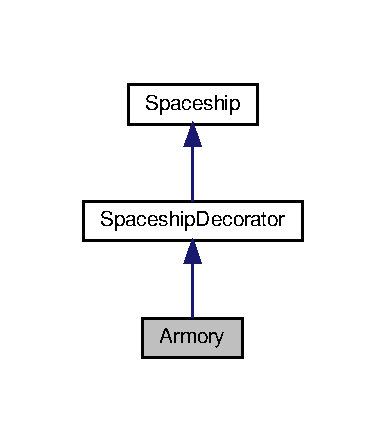
\includegraphics[width=185pt]{classArmory__inherit__graph}
\end{center}
\end{figure}


Collaboration diagram for Armory\+:\nopagebreak
\begin{figure}[H]
\begin{center}
\leavevmode
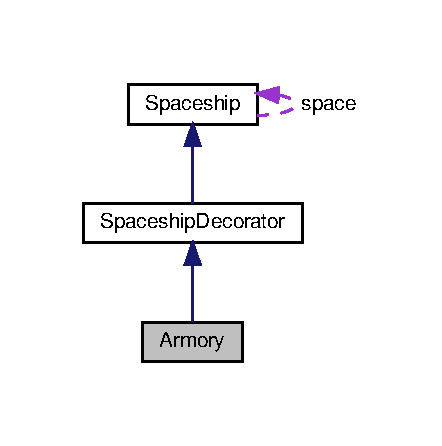
\includegraphics[width=212pt]{classArmory__coll__graph}
\end{center}
\end{figure}
\subsection*{Public Member Functions}
\begin{DoxyCompactItemize}
\item 
\hyperlink{classArmory_ad1d556c807fe5f3e5852cfbb818c4f1c}{Armory} ()
\item 
\hyperlink{classArmory_a4af8efb475734ef6292e5cdef489c9d9}{$\sim$\+Armory} ()
\item 
void \hyperlink{classArmory_adccb51a0901294546bfb1da350ae6836}{add\+Ship} (\hyperlink{classSpaceship}{Spaceship} $\ast$s)
\item 
double \hyperlink{classArmory_a06bba21799ef0b2a9f835632411420a4}{get\+Resources} (double a, double b)
\item 
void \hyperlink{classArmory_a76e105e23137e82f67e752ff13f52d75}{visit} (\hyperlink{classPlanet}{Planet} $\ast$p)
\item 
\hyperlink{classMemento}{Memento} $\ast$ \hyperlink{classArmory_aba8aa540182986fbb0ca8a741f491ffe}{create\+Memento} (vector$<$ \hyperlink{classSpaceship}{Spaceship} $\ast$$>$ s)
\item 
void \hyperlink{classArmory_ad4027c724be016da41eeac5aaab2238b}{reinstate\+Memento} (\hyperlink{classMemento}{Memento} $\ast$mem)
\item 
void \hyperlink{classArmory_aab75c86069fac4995a56c6318a33e504}{execute\+Strategy} ()
\item 
void \hyperlink{classArmory_a85d472873bf4ce934c849f7c362f7064}{select\+Strategy} (\hyperlink{classStrategy}{Strategy} $\ast$s)
\end{DoxyCompactItemize}
\subsection*{Additional Inherited Members}


\subsection{Detailed Description}
\hyperlink{classArmory}{Armory} class. 

\subsection{Constructor \& Destructor Documentation}
\mbox{\Hypertarget{classArmory_ad1d556c807fe5f3e5852cfbb818c4f1c}\label{classArmory_ad1d556c807fe5f3e5852cfbb818c4f1c}} 
\index{Armory@{Armory}!Armory@{Armory}}
\index{Armory@{Armory}!Armory@{Armory}}
\subsubsection{\texorpdfstring{Armory()}{Armory()}}
{\footnotesize\ttfamily Armory\+::\+Armory (\begin{DoxyParamCaption}{ }\end{DoxyParamCaption})}

Default constructor \mbox{\Hypertarget{classArmory_a4af8efb475734ef6292e5cdef489c9d9}\label{classArmory_a4af8efb475734ef6292e5cdef489c9d9}} 
\index{Armory@{Armory}!````~Armory@{$\sim$\+Armory}}
\index{````~Armory@{$\sim$\+Armory}!Armory@{Armory}}
\subsubsection{\texorpdfstring{$\sim$\+Armory()}{~Armory()}}
{\footnotesize\ttfamily Armory\+::$\sim$\+Armory (\begin{DoxyParamCaption}{ }\end{DoxyParamCaption})}

Default destructor 

\subsection{Member Function Documentation}
\mbox{\Hypertarget{classArmory_adccb51a0901294546bfb1da350ae6836}\label{classArmory_adccb51a0901294546bfb1da350ae6836}} 
\index{Armory@{Armory}!add\+Ship@{add\+Ship}}
\index{add\+Ship@{add\+Ship}!Armory@{Armory}}
\subsubsection{\texorpdfstring{add\+Ship()}{addShip()}}
{\footnotesize\ttfamily void Armory\+::add\+Ship (\begin{DoxyParamCaption}\item[{\hyperlink{classSpaceship}{Spaceship} $\ast$}]{s }\end{DoxyParamCaption})\hspace{0.3cm}{\ttfamily [inline]}, {\ttfamily [virtual]}}

Virtual add\+Ship 

Reimplemented from \hyperlink{classSpaceshipDecorator_a5ed39419f5fab65dd4af11bf5136f7a4}{Spaceship\+Decorator}.

\mbox{\Hypertarget{classArmory_aba8aa540182986fbb0ca8a741f491ffe}\label{classArmory_aba8aa540182986fbb0ca8a741f491ffe}} 
\index{Armory@{Armory}!create\+Memento@{create\+Memento}}
\index{create\+Memento@{create\+Memento}!Armory@{Armory}}
\subsubsection{\texorpdfstring{create\+Memento()}{createMemento()}}
{\footnotesize\ttfamily \hyperlink{classMemento}{Memento}$\ast$ Armory\+::create\+Memento (\begin{DoxyParamCaption}\item[{vector$<$ \hyperlink{classSpaceship}{Spaceship} $\ast$$>$}]{s }\end{DoxyParamCaption})\hspace{0.3cm}{\ttfamily [inline]}, {\ttfamily [virtual]}}

create memento stub 

Reimplemented from \hyperlink{classSpaceship_a6d272f846b019dec8226ddab65648a7b}{Spaceship}.

\mbox{\Hypertarget{classArmory_aab75c86069fac4995a56c6318a33e504}\label{classArmory_aab75c86069fac4995a56c6318a33e504}} 
\index{Armory@{Armory}!execute\+Strategy@{execute\+Strategy}}
\index{execute\+Strategy@{execute\+Strategy}!Armory@{Armory}}
\subsubsection{\texorpdfstring{execute\+Strategy()}{executeStrategy()}}
{\footnotesize\ttfamily void Armory\+::execute\+Strategy (\begin{DoxyParamCaption}{ }\end{DoxyParamCaption})\hspace{0.3cm}{\ttfamily [inline]}, {\ttfamily [virtual]}}

execute strategy 

Reimplemented from \hyperlink{classSpaceship}{Spaceship}.

\mbox{\Hypertarget{classArmory_a06bba21799ef0b2a9f835632411420a4}\label{classArmory_a06bba21799ef0b2a9f835632411420a4}} 
\index{Armory@{Armory}!get\+Resources@{get\+Resources}}
\index{get\+Resources@{get\+Resources}!Armory@{Armory}}
\subsubsection{\texorpdfstring{get\+Resources()}{getResources()}}
{\footnotesize\ttfamily double Armory\+::get\+Resources (\begin{DoxyParamCaption}\item[{double}]{a,  }\item[{double}]{b }\end{DoxyParamCaption})\hspace{0.3cm}{\ttfamily [inline]}, {\ttfamily [virtual]}}

stub resource collection 

Reimplemented from \hyperlink{classSpaceshipDecorator_a5ee7a9a8c146c85f08591e47d971dce7}{Spaceship\+Decorator}.

\mbox{\Hypertarget{classArmory_ad4027c724be016da41eeac5aaab2238b}\label{classArmory_ad4027c724be016da41eeac5aaab2238b}} 
\index{Armory@{Armory}!reinstate\+Memento@{reinstate\+Memento}}
\index{reinstate\+Memento@{reinstate\+Memento}!Armory@{Armory}}
\subsubsection{\texorpdfstring{reinstate\+Memento()}{reinstateMemento()}}
{\footnotesize\ttfamily void Armory\+::reinstate\+Memento (\begin{DoxyParamCaption}\item[{\hyperlink{classMemento}{Memento} $\ast$}]{mem }\end{DoxyParamCaption})\hspace{0.3cm}{\ttfamily [inline]}, {\ttfamily [virtual]}}

reinstate memento 

Reimplemented from \hyperlink{classSpaceship_ab075c869473344b6471c8e28ca7ea61e}{Spaceship}.

\mbox{\Hypertarget{classArmory_a85d472873bf4ce934c849f7c362f7064}\label{classArmory_a85d472873bf4ce934c849f7c362f7064}} 
\index{Armory@{Armory}!select\+Strategy@{select\+Strategy}}
\index{select\+Strategy@{select\+Strategy}!Armory@{Armory}}
\subsubsection{\texorpdfstring{select\+Strategy()}{selectStrategy()}}
{\footnotesize\ttfamily void Armory\+::select\+Strategy (\begin{DoxyParamCaption}\item[{\hyperlink{classStrategy}{Strategy} $\ast$}]{s }\end{DoxyParamCaption})\hspace{0.3cm}{\ttfamily [inline]}, {\ttfamily [virtual]}}

select strategy 

Reimplemented from \hyperlink{classSpaceship_a93be2d9d2b675ef978d866d4cd7a6524}{Spaceship}.

\mbox{\Hypertarget{classArmory_a76e105e23137e82f67e752ff13f52d75}\label{classArmory_a76e105e23137e82f67e752ff13f52d75}} 
\index{Armory@{Armory}!visit@{visit}}
\index{visit@{visit}!Armory@{Armory}}
\subsubsection{\texorpdfstring{visit()}{visit()}}
{\footnotesize\ttfamily void Armory\+::visit (\begin{DoxyParamCaption}\item[{\hyperlink{classPlanet}{Planet} $\ast$}]{p }\end{DoxyParamCaption})\hspace{0.3cm}{\ttfamily [inline]}, {\ttfamily [virtual]}}

stub for visit 

Reimplemented from \hyperlink{classSpaceship}{Spaceship}.



The documentation for this class was generated from the following files\+:\begin{DoxyCompactItemize}
\item 
Armory.\+h\item 
Armory.\+cpp\end{DoxyCompactItemize}

\hypertarget{classBattleship}{}\section{Battleship Class Reference}
\label{classBattleship}\index{Battleship@{Battleship}}


\hyperlink{classBattleship}{Battleship} class.  




{\ttfamily \#include $<$Battleship.\+h$>$}



Inheritance diagram for Battleship\+:\nopagebreak
\begin{figure}[H]
\begin{center}
\leavevmode
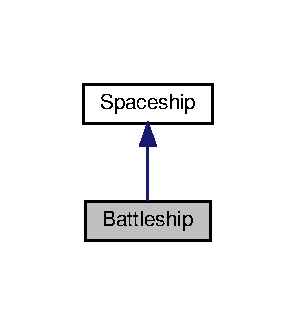
\includegraphics[width=142pt]{classBattleship__inherit__graph}
\end{center}
\end{figure}


Collaboration diagram for Battleship\+:\nopagebreak
\begin{figure}[H]
\begin{center}
\leavevmode
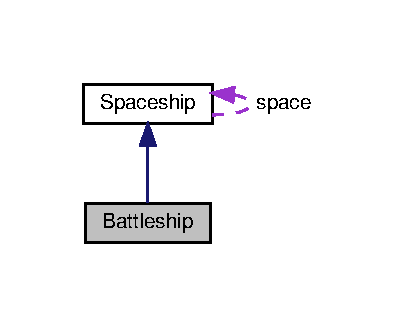
\includegraphics[width=190pt]{classBattleship__coll__graph}
\end{center}
\end{figure}
\subsection*{Public Member Functions}
\begin{DoxyCompactItemize}
\item 
\hyperlink{classBattleship_a57a0db9eadfe53049035b3b0e5ec5367}{Battleship} ()
\item 
\hyperlink{classBattleship_afdc3250fb22d1d2dac6f1f71041888c4}{Battleship} (string name)
\item 
virtual void \hyperlink{classBattleship_a698e2d0ef1ffa4e6b5e7b09c0ff7d07c}{add\+Component} (\hyperlink{classSpaceship}{Spaceship} $\ast$comp)
\item 
int \hyperlink{classBattleship_a5fadf030665554b56456467e98c75228}{get\+Type} ()
\item 
void \hyperlink{classBattleship_af89b875b0dadcbf79b6d65d97398e7c1}{visit} (\hyperlink{classPlanet}{Planet} $\ast$p)
\item 
void \hyperlink{classBattleship_a4db634686a840f3348c2a124e5f42d66}{increase\+Threat\+Level} ()
\item 
void \hyperlink{classBattleship_a31ab6421ece477f4de7989b31aa8ed02}{decrease\+Threat\+Level} ()
\item 
void \hyperlink{classBattleship_a41f44a1437e169165b943c3b98316f32}{print\+Threat\+Level} ()
\item 
void \hyperlink{classBattleship_acbb94a57bb20013b07686b750985eb9e}{execute\+Strategy} ()
\item 
void \hyperlink{classBattleship_a2a729de36df2648305cb68c9779c9c2e}{select\+Strategy} (\hyperlink{classStrategy}{Strategy} $\ast$s)
\item 
void \hyperlink{classBattleship_a9167350d564a8f8286841408f0bacdf9}{add\+Ship} (\hyperlink{classSpaceship}{Spaceship} $\ast$s)
\item 
double \hyperlink{classBattleship_a91c6d577c5c761b607b204a9fc59c3ad}{get\+Resources} (double a, double b)
\item 
\hyperlink{classMemento}{Memento} $\ast$ \hyperlink{classBattleship_a0e039fa419a67ff2fec0e65d93f2fefd}{create\+Memento} (vector$<$ \hyperlink{classSpaceship}{Spaceship} $\ast$$>$ s)
\item 
void \hyperlink{classBattleship_a46f7920029ef4968db3a4429f0fb9372}{reinstate\+Memento} (\hyperlink{classMemento}{Memento} $\ast$mem)
\end{DoxyCompactItemize}
\subsection*{Additional Inherited Members}


\subsection{Detailed Description}
\hyperlink{classBattleship}{Battleship} class. 

\subsection{Constructor \& Destructor Documentation}
\mbox{\Hypertarget{classBattleship_a57a0db9eadfe53049035b3b0e5ec5367}\label{classBattleship_a57a0db9eadfe53049035b3b0e5ec5367}} 
\index{Battleship@{Battleship}!Battleship@{Battleship}}
\index{Battleship@{Battleship}!Battleship@{Battleship}}
\subsubsection{\texorpdfstring{Battleship()}{Battleship()}\hspace{0.1cm}{\footnotesize\ttfamily [1/2]}}
{\footnotesize\ttfamily Battleship\+::\+Battleship (\begin{DoxyParamCaption}{ }\end{DoxyParamCaption})\hspace{0.3cm}{\ttfamily [inline]}}

Default constructor \mbox{\Hypertarget{classBattleship_afdc3250fb22d1d2dac6f1f71041888c4}\label{classBattleship_afdc3250fb22d1d2dac6f1f71041888c4}} 
\index{Battleship@{Battleship}!Battleship@{Battleship}}
\index{Battleship@{Battleship}!Battleship@{Battleship}}
\subsubsection{\texorpdfstring{Battleship()}{Battleship()}\hspace{0.1cm}{\footnotesize\ttfamily [2/2]}}
{\footnotesize\ttfamily Battleship\+::\+Battleship (\begin{DoxyParamCaption}\item[{string}]{name }\end{DoxyParamCaption})\hspace{0.3cm}{\ttfamily [inline]}}

Default desctructor\+Paramaterised constructor 

\subsection{Member Function Documentation}
\mbox{\Hypertarget{classBattleship_a698e2d0ef1ffa4e6b5e7b09c0ff7d07c}\label{classBattleship_a698e2d0ef1ffa4e6b5e7b09c0ff7d07c}} 
\index{Battleship@{Battleship}!add\+Component@{add\+Component}}
\index{add\+Component@{add\+Component}!Battleship@{Battleship}}
\subsubsection{\texorpdfstring{add\+Component()}{addComponent()}}
{\footnotesize\ttfamily virtual void Battleship\+::add\+Component (\begin{DoxyParamCaption}\item[{\hyperlink{classSpaceship}{Spaceship} $\ast$}]{comp }\end{DoxyParamCaption})\hspace{0.3cm}{\ttfamily [inline]}, {\ttfamily [virtual]}}

Add a component 

Implements \hyperlink{classSpaceship_ac1b4673a691cd100708ddea08cd9f192}{Spaceship}.

\mbox{\Hypertarget{classBattleship_a9167350d564a8f8286841408f0bacdf9}\label{classBattleship_a9167350d564a8f8286841408f0bacdf9}} 
\index{Battleship@{Battleship}!add\+Ship@{add\+Ship}}
\index{add\+Ship@{add\+Ship}!Battleship@{Battleship}}
\subsubsection{\texorpdfstring{add\+Ship()}{addShip()}}
{\footnotesize\ttfamily void Battleship\+::add\+Ship (\begin{DoxyParamCaption}\item[{\hyperlink{classSpaceship}{Spaceship} $\ast$}]{ }\end{DoxyParamCaption})\hspace{0.3cm}{\ttfamily [inline]}, {\ttfamily [virtual]}}

Virtual add\+Ship 

Reimplemented from \hyperlink{classSpaceship_a90e1321cdbcb459b98b75ab39cef867d}{Spaceship}.

\mbox{\Hypertarget{classBattleship_a0e039fa419a67ff2fec0e65d93f2fefd}\label{classBattleship_a0e039fa419a67ff2fec0e65d93f2fefd}} 
\index{Battleship@{Battleship}!create\+Memento@{create\+Memento}}
\index{create\+Memento@{create\+Memento}!Battleship@{Battleship}}
\subsubsection{\texorpdfstring{create\+Memento()}{createMemento()}}
{\footnotesize\ttfamily \hyperlink{classMemento}{Memento}$\ast$ Battleship\+::create\+Memento (\begin{DoxyParamCaption}\item[{vector$<$ \hyperlink{classSpaceship}{Spaceship} $\ast$$>$}]{s }\end{DoxyParamCaption})\hspace{0.3cm}{\ttfamily [inline]}, {\ttfamily [virtual]}}

create memento stub 

Reimplemented from \hyperlink{classSpaceship_a6d272f846b019dec8226ddab65648a7b}{Spaceship}.

\mbox{\Hypertarget{classBattleship_a31ab6421ece477f4de7989b31aa8ed02}\label{classBattleship_a31ab6421ece477f4de7989b31aa8ed02}} 
\index{Battleship@{Battleship}!decrease\+Threat\+Level@{decrease\+Threat\+Level}}
\index{decrease\+Threat\+Level@{decrease\+Threat\+Level}!Battleship@{Battleship}}
\subsubsection{\texorpdfstring{decrease\+Threat\+Level()}{decreaseThreatLevel()}}
{\footnotesize\ttfamily void Battleship\+::decrease\+Threat\+Level (\begin{DoxyParamCaption}{ }\end{DoxyParamCaption})\hspace{0.3cm}{\ttfamily [inline]}, {\ttfamily [virtual]}}

stub for decrease\+Threat\+Level 

Reimplemented from \hyperlink{classSpaceship_a73a1eefd211e9a2063d924ee85f0c0c7}{Spaceship}.

\mbox{\Hypertarget{classBattleship_acbb94a57bb20013b07686b750985eb9e}\label{classBattleship_acbb94a57bb20013b07686b750985eb9e}} 
\index{Battleship@{Battleship}!execute\+Strategy@{execute\+Strategy}}
\index{execute\+Strategy@{execute\+Strategy}!Battleship@{Battleship}}
\subsubsection{\texorpdfstring{execute\+Strategy()}{executeStrategy()}}
{\footnotesize\ttfamily void Battleship\+::execute\+Strategy (\begin{DoxyParamCaption}{ }\end{DoxyParamCaption})\hspace{0.3cm}{\ttfamily [inline]}, {\ttfamily [virtual]}}

execute strategy 

Reimplemented from \hyperlink{classSpaceship}{Spaceship}.

\mbox{\Hypertarget{classBattleship_a91c6d577c5c761b607b204a9fc59c3ad}\label{classBattleship_a91c6d577c5c761b607b204a9fc59c3ad}} 
\index{Battleship@{Battleship}!get\+Resources@{get\+Resources}}
\index{get\+Resources@{get\+Resources}!Battleship@{Battleship}}
\subsubsection{\texorpdfstring{get\+Resources()}{getResources()}}
{\footnotesize\ttfamily double Battleship\+::get\+Resources (\begin{DoxyParamCaption}\item[{double}]{a,  }\item[{double}]{b }\end{DoxyParamCaption})\hspace{0.3cm}{\ttfamily [inline]}, {\ttfamily [virtual]}}

stub resource collection 

Reimplemented from \hyperlink{classSpaceship_ad2027533de1d789db5e3efa22055f2d0}{Spaceship}.

\mbox{\Hypertarget{classBattleship_a5fadf030665554b56456467e98c75228}\label{classBattleship_a5fadf030665554b56456467e98c75228}} 
\index{Battleship@{Battleship}!get\+Type@{get\+Type}}
\index{get\+Type@{get\+Type}!Battleship@{Battleship}}
\subsubsection{\texorpdfstring{get\+Type()}{getType()}}
{\footnotesize\ttfamily int Battleship\+::get\+Type (\begin{DoxyParamCaption}{ }\end{DoxyParamCaption})\hspace{0.3cm}{\ttfamily [inline]}, {\ttfamily [virtual]}}

Get the type of spaceship \hyperlink{classBattleship}{Battleship} = 1 \begin{DoxyReturn}{Returns}
int -\/ 1 
\end{DoxyReturn}


Reimplemented from \hyperlink{classSpaceship_a113055e6d793f8fbc55e44efc4d57e07}{Spaceship}.

\mbox{\Hypertarget{classBattleship_a4db634686a840f3348c2a124e5f42d66}\label{classBattleship_a4db634686a840f3348c2a124e5f42d66}} 
\index{Battleship@{Battleship}!increase\+Threat\+Level@{increase\+Threat\+Level}}
\index{increase\+Threat\+Level@{increase\+Threat\+Level}!Battleship@{Battleship}}
\subsubsection{\texorpdfstring{increase\+Threat\+Level()}{increaseThreatLevel()}}
{\footnotesize\ttfamily void Battleship\+::increase\+Threat\+Level (\begin{DoxyParamCaption}{ }\end{DoxyParamCaption})\hspace{0.3cm}{\ttfamily [inline]}, {\ttfamily [virtual]}}

stub for increase\+Threat\+Level 

Reimplemented from \hyperlink{classSpaceship_a5ddf702124286d9d3a6b5e64c09515bc}{Spaceship}.

\mbox{\Hypertarget{classBattleship_a41f44a1437e169165b943c3b98316f32}\label{classBattleship_a41f44a1437e169165b943c3b98316f32}} 
\index{Battleship@{Battleship}!print\+Threat\+Level@{print\+Threat\+Level}}
\index{print\+Threat\+Level@{print\+Threat\+Level}!Battleship@{Battleship}}
\subsubsection{\texorpdfstring{print\+Threat\+Level()}{printThreatLevel()}}
{\footnotesize\ttfamily void Battleship\+::print\+Threat\+Level (\begin{DoxyParamCaption}{ }\end{DoxyParamCaption})\hspace{0.3cm}{\ttfamily [inline]}, {\ttfamily [virtual]}}

stub for print\+Threat\+Level 

Reimplemented from \hyperlink{classSpaceship_a8f16814f888a5a1423e5a491329cdb97}{Spaceship}.

\mbox{\Hypertarget{classBattleship_a46f7920029ef4968db3a4429f0fb9372}\label{classBattleship_a46f7920029ef4968db3a4429f0fb9372}} 
\index{Battleship@{Battleship}!reinstate\+Memento@{reinstate\+Memento}}
\index{reinstate\+Memento@{reinstate\+Memento}!Battleship@{Battleship}}
\subsubsection{\texorpdfstring{reinstate\+Memento()}{reinstateMemento()}}
{\footnotesize\ttfamily void Battleship\+::reinstate\+Memento (\begin{DoxyParamCaption}\item[{\hyperlink{classMemento}{Memento} $\ast$}]{mem }\end{DoxyParamCaption})\hspace{0.3cm}{\ttfamily [inline]}, {\ttfamily [virtual]}}

reinstate memento 

Reimplemented from \hyperlink{classSpaceship_ab075c869473344b6471c8e28ca7ea61e}{Spaceship}.

\mbox{\Hypertarget{classBattleship_a2a729de36df2648305cb68c9779c9c2e}\label{classBattleship_a2a729de36df2648305cb68c9779c9c2e}} 
\index{Battleship@{Battleship}!select\+Strategy@{select\+Strategy}}
\index{select\+Strategy@{select\+Strategy}!Battleship@{Battleship}}
\subsubsection{\texorpdfstring{select\+Strategy()}{selectStrategy()}}
{\footnotesize\ttfamily void Battleship\+::select\+Strategy (\begin{DoxyParamCaption}\item[{\hyperlink{classStrategy}{Strategy} $\ast$}]{s }\end{DoxyParamCaption})\hspace{0.3cm}{\ttfamily [inline]}, {\ttfamily [virtual]}}

select strategy 

Reimplemented from \hyperlink{classSpaceship_a93be2d9d2b675ef978d866d4cd7a6524}{Spaceship}.

\mbox{\Hypertarget{classBattleship_af89b875b0dadcbf79b6d65d97398e7c1}\label{classBattleship_af89b875b0dadcbf79b6d65d97398e7c1}} 
\index{Battleship@{Battleship}!visit@{visit}}
\index{visit@{visit}!Battleship@{Battleship}}
\subsubsection{\texorpdfstring{visit()}{visit()}}
{\footnotesize\ttfamily void Battleship\+::visit (\begin{DoxyParamCaption}\item[{\hyperlink{classPlanet}{Planet} $\ast$}]{p }\end{DoxyParamCaption})\hspace{0.3cm}{\ttfamily [inline]}, {\ttfamily [virtual]}}

stub for visit 

Reimplemented from \hyperlink{classSpaceship}{Spaceship}.



The documentation for this class was generated from the following file\+:\begin{DoxyCompactItemize}
\item 
Battleship.\+h\end{DoxyCompactItemize}

\hypertarget{classBattleshipFactory}{}\section{Battleship\+Factory Class Reference}
\label{classBattleshipFactory}\index{Battleship\+Factory@{Battleship\+Factory}}


\hyperlink{classBattleship}{Battleship} Factory class.  




{\ttfamily \#include $<$Battleship\+Factory.\+h$>$}



Inheritance diagram for Battleship\+Factory\+:\nopagebreak
\begin{figure}[H]
\begin{center}
\leavevmode
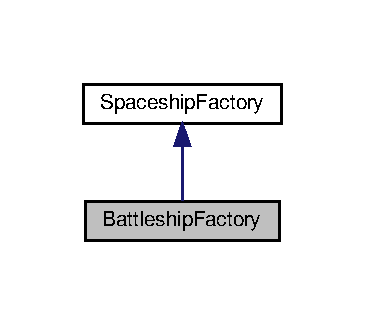
\includegraphics[width=175pt]{classBattleshipFactory__inherit__graph}
\end{center}
\end{figure}


Collaboration diagram for Battleship\+Factory\+:\nopagebreak
\begin{figure}[H]
\begin{center}
\leavevmode
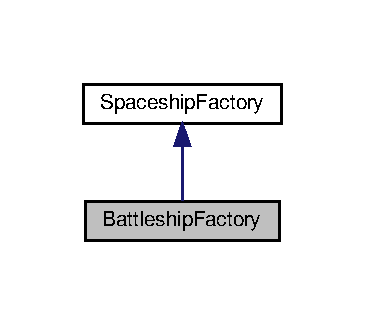
\includegraphics[width=175pt]{classBattleshipFactory__coll__graph}
\end{center}
\end{figure}
\subsection*{Public Member Functions}
\begin{DoxyCompactItemize}
\item 
\hyperlink{classBattleshipFactory_a98f1b363d37b3dcaaf066ba6f3dca375}{Battleship\+Factory} ()
\item 
\hyperlink{classBattleshipFactory_a18d29d1462e12301c49c2632144ff5e4}{$\sim$\+Battleship\+Factory} ()
\item 
\hyperlink{classSpaceship}{Spaceship} $\ast$ \hyperlink{classBattleshipFactory_a1d85420a3be7db3e96e9c8b33a387330}{space\+Ship\+Factory\+Method} (string n)
\end{DoxyCompactItemize}


\subsection{Detailed Description}
\hyperlink{classBattleship}{Battleship} Factory class. 

\subsection{Constructor \& Destructor Documentation}
\mbox{\Hypertarget{classBattleshipFactory_a98f1b363d37b3dcaaf066ba6f3dca375}\label{classBattleshipFactory_a98f1b363d37b3dcaaf066ba6f3dca375}} 
\index{Battleship\+Factory@{Battleship\+Factory}!Battleship\+Factory@{Battleship\+Factory}}
\index{Battleship\+Factory@{Battleship\+Factory}!Battleship\+Factory@{Battleship\+Factory}}
\subsubsection{\texorpdfstring{Battleship\+Factory()}{BattleshipFactory()}}
{\footnotesize\ttfamily Battleship\+Factory\+::\+Battleship\+Factory (\begin{DoxyParamCaption}{ }\end{DoxyParamCaption})}

Default constructor \mbox{\Hypertarget{classBattleshipFactory_a18d29d1462e12301c49c2632144ff5e4}\label{classBattleshipFactory_a18d29d1462e12301c49c2632144ff5e4}} 
\index{Battleship\+Factory@{Battleship\+Factory}!````~Battleship\+Factory@{$\sim$\+Battleship\+Factory}}
\index{````~Battleship\+Factory@{$\sim$\+Battleship\+Factory}!Battleship\+Factory@{Battleship\+Factory}}
\subsubsection{\texorpdfstring{$\sim$\+Battleship\+Factory()}{~BattleshipFactory()}}
{\footnotesize\ttfamily Battleship\+Factory\+::$\sim$\+Battleship\+Factory (\begin{DoxyParamCaption}{ }\end{DoxyParamCaption})}

Defauly desctructor 

\subsection{Member Function Documentation}
\mbox{\Hypertarget{classBattleshipFactory_a1d85420a3be7db3e96e9c8b33a387330}\label{classBattleshipFactory_a1d85420a3be7db3e96e9c8b33a387330}} 
\index{Battleship\+Factory@{Battleship\+Factory}!space\+Ship\+Factory\+Method@{space\+Ship\+Factory\+Method}}
\index{space\+Ship\+Factory\+Method@{space\+Ship\+Factory\+Method}!Battleship\+Factory@{Battleship\+Factory}}
\subsubsection{\texorpdfstring{space\+Ship\+Factory\+Method()}{spaceShipFactoryMethod()}}
{\footnotesize\ttfamily \hyperlink{classSpaceship}{Spaceship} $\ast$ Battleship\+Factory\+::space\+Ship\+Factory\+Method (\begin{DoxyParamCaption}\item[{string}]{n }\end{DoxyParamCaption})\hspace{0.3cm}{\ttfamily [virtual]}}

Method to create Battleships \begin{DoxyReturn}{Returns}
new spaceship 
\end{DoxyReturn}


Implements \hyperlink{classSpaceshipFactory_a70b50dd616cb16f50088eff9ca07cda9}{Spaceship\+Factory}.



The documentation for this class was generated from the following files\+:\begin{DoxyCompactItemize}
\item 
Battleship\+Factory.\+h\item 
Battleship\+Factory.\+cpp\end{DoxyCompactItemize}

\hypertarget{classBridge}{}\section{Bridge Class Reference}
\label{classBridge}\index{Bridge@{Bridge}}


\hyperlink{classBridge}{Bridge} class.  




{\ttfamily \#include $<$Bridge.\+h$>$}



Inheritance diagram for Bridge\+:
% FIG 0


Collaboration diagram for Bridge\+:
% FIG 1
\subsection*{Public Member Functions}
\begin{DoxyCompactItemize}
\item 
\hyperlink{classBridge_a275f54dafc95c9b5bbaba5e904c4fa9a}{Bridge} ()
\item 
\hyperlink{classBridge_a31994152fc209370604140c3591339c9}{Bridge} (\hyperlink{classStrategy}{Strategy} $\ast$s)
\item 
\hyperlink{classBridge_a812b325fbb4f4b589e68f11f443a7ee4}{$\sim$\+Bridge} ()
\item 
double \hyperlink{classBridge_a1508c1c9cfb44850fea31afcb7f1e403}{get\+Resources} (double a, double b)
\end{DoxyCompactItemize}
\subsection*{Additional Inherited Members}


\subsection{Detailed Description}
\hyperlink{classBridge}{Bridge} class. 

\subsection{Constructor \& Destructor Documentation}
\mbox{\Hypertarget{classBridge_a275f54dafc95c9b5bbaba5e904c4fa9a}\label{classBridge_a275f54dafc95c9b5bbaba5e904c4fa9a}} 
\index{Bridge@{Bridge}!Bridge@{Bridge}}
\index{Bridge@{Bridge}!Bridge@{Bridge}}
\subsubsection{\texorpdfstring{Bridge()}{Bridge()}\hspace{0.1cm}{\footnotesize\ttfamily [1/2]}}
{\footnotesize\ttfamily Bridge\+::\+Bridge (\begin{DoxyParamCaption}{ }\end{DoxyParamCaption})}

Default constructor \mbox{\Hypertarget{classBridge_a31994152fc209370604140c3591339c9}\label{classBridge_a31994152fc209370604140c3591339c9}} 
\index{Bridge@{Bridge}!Bridge@{Bridge}}
\index{Bridge@{Bridge}!Bridge@{Bridge}}
\subsubsection{\texorpdfstring{Bridge()}{Bridge()}\hspace{0.1cm}{\footnotesize\ttfamily [2/2]}}
{\footnotesize\ttfamily Bridge\+::\+Bridge (\begin{DoxyParamCaption}\item[{\hyperlink{classStrategy}{Strategy} $\ast$}]{s }\end{DoxyParamCaption})}

Paramaterised constructor \mbox{\Hypertarget{classBridge_a812b325fbb4f4b589e68f11f443a7ee4}\label{classBridge_a812b325fbb4f4b589e68f11f443a7ee4}} 
\index{Bridge@{Bridge}!````~Bridge@{$\sim$\+Bridge}}
\index{````~Bridge@{$\sim$\+Bridge}!Bridge@{Bridge}}
\subsubsection{\texorpdfstring{$\sim$\+Bridge()}{~Bridge()}}
{\footnotesize\ttfamily Bridge\+::$\sim$\+Bridge (\begin{DoxyParamCaption}{ }\end{DoxyParamCaption})}

Default destructor 

\subsection{Member Function Documentation}
\mbox{\Hypertarget{classBridge_a1508c1c9cfb44850fea31afcb7f1e403}\label{classBridge_a1508c1c9cfb44850fea31afcb7f1e403}} 
\index{Bridge@{Bridge}!get\+Resources@{get\+Resources}}
\index{get\+Resources@{get\+Resources}!Bridge@{Bridge}}
\subsubsection{\texorpdfstring{get\+Resources()}{getResources()}}
{\footnotesize\ttfamily double Bridge\+::get\+Resources (\begin{DoxyParamCaption}\item[{double}]{a,  }\item[{double}]{b }\end{DoxyParamCaption})}

resource collection 

The documentation for this class was generated from the following files\+:\begin{DoxyCompactItemize}
\item 
Bridge.\+h\item 
Bridge.\+cpp\end{DoxyCompactItemize}

\hypertarget{classCaptain}{}\section{Captain Class Reference}
\label{classCaptain}\index{Captain@{Captain}}


\hyperlink{classCaptain}{Captain} class.  




{\ttfamily \#include $<$Captain.\+h$>$}



Inheritance diagram for Captain\+:\nopagebreak
\begin{figure}[H]
\begin{center}
\leavevmode
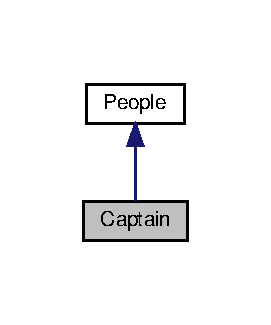
\includegraphics[width=130pt]{classCaptain__inherit__graph}
\end{center}
\end{figure}


Collaboration diagram for Captain\+:\nopagebreak
\begin{figure}[H]
\begin{center}
\leavevmode
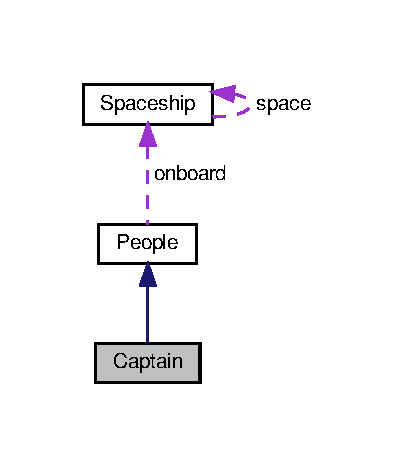
\includegraphics[width=190pt]{classCaptain__coll__graph}
\end{center}
\end{figure}
\subsection*{Public Member Functions}
\begin{DoxyCompactItemize}
\item 
\hyperlink{classCaptain_a097ac4126a1320400460628a3ed2f376}{Captain} ()
\item 
\hyperlink{classCaptain_a6b8671d624f45a11b7fd33f5ff9a6930}{$\sim$\+Captain} ()
\item 
void \hyperlink{classCaptain_a39ebd40ec094b410f295188bb6262009}{recieve\+Spaceship\+Error} (string)
\item 
void \hyperlink{classCaptain_a88abc1940bcdef8a655efc20ebd68d50}{send\+Error\+Message} (string)
\item 
string \hyperlink{classCaptain_a87ae1c47127aec69cc58133d82e488d3}{get\+Type} ()
\end{DoxyCompactItemize}
\subsection*{Additional Inherited Members}


\subsection{Detailed Description}
\hyperlink{classCaptain}{Captain} class. 

\subsection{Constructor \& Destructor Documentation}
\mbox{\Hypertarget{classCaptain_a097ac4126a1320400460628a3ed2f376}\label{classCaptain_a097ac4126a1320400460628a3ed2f376}} 
\index{Captain@{Captain}!Captain@{Captain}}
\index{Captain@{Captain}!Captain@{Captain}}
\subsubsection{\texorpdfstring{Captain()}{Captain()}}
{\footnotesize\ttfamily Captain\+::\+Captain (\begin{DoxyParamCaption}{ }\end{DoxyParamCaption})\hspace{0.3cm}{\ttfamily [inline]}}

Default constructor \mbox{\Hypertarget{classCaptain_a6b8671d624f45a11b7fd33f5ff9a6930}\label{classCaptain_a6b8671d624f45a11b7fd33f5ff9a6930}} 
\index{Captain@{Captain}!````~Captain@{$\sim$\+Captain}}
\index{````~Captain@{$\sim$\+Captain}!Captain@{Captain}}
\subsubsection{\texorpdfstring{$\sim$\+Captain()}{~Captain()}}
{\footnotesize\ttfamily Captain\+::$\sim$\+Captain (\begin{DoxyParamCaption}{ }\end{DoxyParamCaption})\hspace{0.3cm}{\ttfamily [inline]}}

Default destructor 

\subsection{Member Function Documentation}
\mbox{\Hypertarget{classCaptain_a87ae1c47127aec69cc58133d82e488d3}\label{classCaptain_a87ae1c47127aec69cc58133d82e488d3}} 
\index{Captain@{Captain}!get\+Type@{get\+Type}}
\index{get\+Type@{get\+Type}!Captain@{Captain}}
\subsubsection{\texorpdfstring{get\+Type()}{getType()}}
{\footnotesize\ttfamily string Captain\+::get\+Type (\begin{DoxyParamCaption}{ }\end{DoxyParamCaption})\hspace{0.3cm}{\ttfamily [inline]}, {\ttfamily [virtual]}}

get type of person 

Implements \hyperlink{classPeople_af60dd882d60cddf63f9b95815ce551a8}{People}.

\mbox{\Hypertarget{classCaptain_a39ebd40ec094b410f295188bb6262009}\label{classCaptain_a39ebd40ec094b410f295188bb6262009}} 
\index{Captain@{Captain}!recieve\+Spaceship\+Error@{recieve\+Spaceship\+Error}}
\index{recieve\+Spaceship\+Error@{recieve\+Spaceship\+Error}!Captain@{Captain}}
\subsubsection{\texorpdfstring{recieve\+Spaceship\+Error()}{recieveSpaceshipError()}}
{\footnotesize\ttfamily void Captain\+::recieve\+Spaceship\+Error (\begin{DoxyParamCaption}\item[{string}]{message }\end{DoxyParamCaption})\hspace{0.3cm}{\ttfamily [virtual]}}

Receive an error from the spaceship 
\begin{DoxyParams}{Parameters}
{\em message} & -\/ The message to be received \\
\hline
\end{DoxyParams}


Implements \hyperlink{classPeople_a0685df78be631783138865e03cc7c85d}{People}.

\mbox{\Hypertarget{classCaptain_a88abc1940bcdef8a655efc20ebd68d50}\label{classCaptain_a88abc1940bcdef8a655efc20ebd68d50}} 
\index{Captain@{Captain}!send\+Error\+Message@{send\+Error\+Message}}
\index{send\+Error\+Message@{send\+Error\+Message}!Captain@{Captain}}
\subsubsection{\texorpdfstring{send\+Error\+Message()}{sendErrorMessage()}}
{\footnotesize\ttfamily void Captain\+::send\+Error\+Message (\begin{DoxyParamCaption}\item[{string}]{message }\end{DoxyParamCaption})\hspace{0.3cm}{\ttfamily [virtual]}}

Send an error to the spaceship 
\begin{DoxyParams}{Parameters}
{\em message} & -\/ The message to be sent \\
\hline
\end{DoxyParams}


Implements \hyperlink{classPeople_a572a35170f61d1848eb04b65baafb057}{People}.



The documentation for this class was generated from the following files\+:\begin{DoxyCompactItemize}
\item 
Captain.\+h\item 
Captain.\+cpp\end{DoxyCompactItemize}

\hypertarget{classCaptainFactory}{}\section{Captain\+Factory Class Reference}
\label{classCaptainFactory}\index{Captain\+Factory@{Captain\+Factory}}


\hyperlink{classCaptain}{Captain} Factory class.  




{\ttfamily \#include $<$Captain\+Factory.\+h$>$}



Inheritance diagram for Captain\+Factory\+:
% FIG 0


Collaboration diagram for Captain\+Factory\+:
% FIG 1
\subsection*{Public Member Functions}
\begin{DoxyCompactItemize}
\item 
\hyperlink{classCaptainFactory_a194bc3adbc4f09ca79df90d1aab30dc1}{Captain\+Factory} ()
\item 
\hyperlink{classCaptainFactory_a1ffe5cdefdefcb36f4c362990dd61080}{$\sim$\+Captain\+Factory} ()
\end{DoxyCompactItemize}


\subsection{Detailed Description}
\hyperlink{classCaptain}{Captain} Factory class. 

\subsection{Constructor \& Destructor Documentation}
\mbox{\Hypertarget{classCaptainFactory_a194bc3adbc4f09ca79df90d1aab30dc1}\label{classCaptainFactory_a194bc3adbc4f09ca79df90d1aab30dc1}} 
\index{Captain\+Factory@{Captain\+Factory}!Captain\+Factory@{Captain\+Factory}}
\index{Captain\+Factory@{Captain\+Factory}!Captain\+Factory@{Captain\+Factory}}
\subsubsection{\texorpdfstring{Captain\+Factory()}{CaptainFactory()}}
{\footnotesize\ttfamily Captain\+Factory\+::\+Captain\+Factory (\begin{DoxyParamCaption}{ }\end{DoxyParamCaption})}

Default constructor \mbox{\Hypertarget{classCaptainFactory_a1ffe5cdefdefcb36f4c362990dd61080}\label{classCaptainFactory_a1ffe5cdefdefcb36f4c362990dd61080}} 
\index{Captain\+Factory@{Captain\+Factory}!````~Captain\+Factory@{$\sim$\+Captain\+Factory}}
\index{````~Captain\+Factory@{$\sim$\+Captain\+Factory}!Captain\+Factory@{Captain\+Factory}}
\subsubsection{\texorpdfstring{$\sim$\+Captain\+Factory()}{~CaptainFactory()}}
{\footnotesize\ttfamily Captain\+Factory\+::$\sim$\+Captain\+Factory (\begin{DoxyParamCaption}{ }\end{DoxyParamCaption})}

Default desctructor 

The documentation for this class was generated from the following file\+:\begin{DoxyCompactItemize}
\item 
Captain\+Factory.\+h\end{DoxyCompactItemize}

\hypertarget{classCaptainsLog}{}\section{Captains\+Log Class Reference}
\label{classCaptainsLog}\index{Captains\+Log@{Captains\+Log}}


Captains Log class.  




{\ttfamily \#include $<$Captains\+Log.\+h$>$}

\subsection*{Public Member Functions}
\begin{DoxyCompactItemize}
\item 
\hyperlink{classCaptainsLog_a79872d886041ecbd5fb13c47fbda825b}{Captains\+Log} ()
\item 
\hyperlink{classCaptainsLog_ad226cf893a8e2498d164be4f6f097231}{$\sim$\+Captains\+Log} ()
\item 
void \hyperlink{classCaptainsLog_a59214274a2c25268a26e2af84fe50bc0}{log\+Event} (string)
\item 
void \hyperlink{classCaptainsLog_a7a534bb9e892210686b76c15b30fab95}{print\+Logs} ()
\end{DoxyCompactItemize}


\subsection{Detailed Description}
Captains Log class. 

\subsection{Constructor \& Destructor Documentation}
\mbox{\Hypertarget{classCaptainsLog_a79872d886041ecbd5fb13c47fbda825b}\label{classCaptainsLog_a79872d886041ecbd5fb13c47fbda825b}} 
\index{Captains\+Log@{Captains\+Log}!Captains\+Log@{Captains\+Log}}
\index{Captains\+Log@{Captains\+Log}!Captains\+Log@{Captains\+Log}}
\subsubsection{\texorpdfstring{Captains\+Log()}{CaptainsLog()}}
{\footnotesize\ttfamily Captains\+Log\+::\+Captains\+Log (\begin{DoxyParamCaption}{ }\end{DoxyParamCaption})}

Default constructor \mbox{\Hypertarget{classCaptainsLog_ad226cf893a8e2498d164be4f6f097231}\label{classCaptainsLog_ad226cf893a8e2498d164be4f6f097231}} 
\index{Captains\+Log@{Captains\+Log}!````~Captains\+Log@{$\sim$\+Captains\+Log}}
\index{````~Captains\+Log@{$\sim$\+Captains\+Log}!Captains\+Log@{Captains\+Log}}
\subsubsection{\texorpdfstring{$\sim$\+Captains\+Log()}{~CaptainsLog()}}
{\footnotesize\ttfamily Captains\+Log\+::$\sim$\+Captains\+Log (\begin{DoxyParamCaption}{ }\end{DoxyParamCaption})}

Default desctructor 

\subsection{Member Function Documentation}
\mbox{\Hypertarget{classCaptainsLog_a59214274a2c25268a26e2af84fe50bc0}\label{classCaptainsLog_a59214274a2c25268a26e2af84fe50bc0}} 
\index{Captains\+Log@{Captains\+Log}!log\+Event@{log\+Event}}
\index{log\+Event@{log\+Event}!Captains\+Log@{Captains\+Log}}
\subsubsection{\texorpdfstring{log\+Event()}{logEvent()}}
{\footnotesize\ttfamily void Captains\+Log\+::log\+Event (\begin{DoxyParamCaption}\item[{string}]{message }\end{DoxyParamCaption})}

Method to add an event to the captains log 
\begin{DoxyParams}{Parameters}
{\em message} & -\/ message to be logged \\
\hline
\end{DoxyParams}
\mbox{\Hypertarget{classCaptainsLog_a7a534bb9e892210686b76c15b30fab95}\label{classCaptainsLog_a7a534bb9e892210686b76c15b30fab95}} 
\index{Captains\+Log@{Captains\+Log}!print\+Logs@{print\+Logs}}
\index{print\+Logs@{print\+Logs}!Captains\+Log@{Captains\+Log}}
\subsubsection{\texorpdfstring{print\+Logs()}{printLogs()}}
{\footnotesize\ttfamily void Captains\+Log\+::print\+Logs (\begin{DoxyParamCaption}{ }\end{DoxyParamCaption})}

Print all logs 

The documentation for this class was generated from the following files\+:\begin{DoxyCompactItemize}
\item 
Captains\+Log.\+h\item 
Captains\+Log.\+cpp\end{DoxyCompactItemize}

\hypertarget{classCaretaker}{}\section{Caretaker Class Reference}
\label{classCaretaker}\index{Caretaker@{Caretaker}}


\hyperlink{classCaretaker}{Caretaker} class.  




{\ttfamily \#include $<$Caretaker.\+h$>$}

\subsection*{Public Member Functions}
\begin{DoxyCompactItemize}
\item 
void \hyperlink{classCaretaker_af818c5b72a75066509b0f61989d67a93}{store\+Memento} (\hyperlink{classMemento}{Memento} $\ast$mem)
\item 
\hyperlink{classMemento}{Memento} $\ast$ \hyperlink{classCaretaker_a1d50fe3b0cbf191f1f260e0bb7f579e6}{retreive\+Memento} ()
\item 
\hyperlink{classCaretaker_a66b14e6d4b79fe9e45051217cee105e8}{$\sim$\+Caretaker} ()
\end{DoxyCompactItemize}


\subsection{Detailed Description}
\hyperlink{classCaretaker}{Caretaker} class. 

\subsection{Constructor \& Destructor Documentation}
\mbox{\Hypertarget{classCaretaker_a66b14e6d4b79fe9e45051217cee105e8}\label{classCaretaker_a66b14e6d4b79fe9e45051217cee105e8}} 
\index{Caretaker@{Caretaker}!````~Caretaker@{$\sim$\+Caretaker}}
\index{````~Caretaker@{$\sim$\+Caretaker}!Caretaker@{Caretaker}}
\subsubsection{\texorpdfstring{$\sim$\+Caretaker()}{~Caretaker()}}
{\footnotesize\ttfamily Caretaker\+::$\sim$\+Caretaker (\begin{DoxyParamCaption}{ }\end{DoxyParamCaption})}

Default destructor 

\subsection{Member Function Documentation}
\mbox{\Hypertarget{classCaretaker_a1d50fe3b0cbf191f1f260e0bb7f579e6}\label{classCaretaker_a1d50fe3b0cbf191f1f260e0bb7f579e6}} 
\index{Caretaker@{Caretaker}!retreive\+Memento@{retreive\+Memento}}
\index{retreive\+Memento@{retreive\+Memento}!Caretaker@{Caretaker}}
\subsubsection{\texorpdfstring{retreive\+Memento()}{retreiveMemento()}}
{\footnotesize\ttfamily \hyperlink{classMemento}{Memento} $\ast$ Caretaker\+::retreive\+Memento (\begin{DoxyParamCaption}{ }\end{DoxyParamCaption})}

Retrieve the memento \begin{DoxyReturn}{Returns}
memento 
\end{DoxyReturn}
\mbox{\Hypertarget{classCaretaker_af818c5b72a75066509b0f61989d67a93}\label{classCaretaker_af818c5b72a75066509b0f61989d67a93}} 
\index{Caretaker@{Caretaker}!store\+Memento@{store\+Memento}}
\index{store\+Memento@{store\+Memento}!Caretaker@{Caretaker}}
\subsubsection{\texorpdfstring{store\+Memento()}{storeMemento()}}
{\footnotesize\ttfamily void Caretaker\+::store\+Memento (\begin{DoxyParamCaption}\item[{\hyperlink{classMemento}{Memento} $\ast$}]{mem }\end{DoxyParamCaption})}

Store the memento 
\begin{DoxyParams}{Parameters}
{\em mem} & -\/ memento to be stored \\
\hline
\end{DoxyParams}


The documentation for this class was generated from the following files\+:\begin{DoxyCompactItemize}
\item 
Caretaker.\+h\item 
Caretaker.\+cpp\end{DoxyCompactItemize}

\hypertarget{classCheifEngineerFactory}{}\section{Cheif\+Engineer\+Factory Class Reference}
\label{classCheifEngineerFactory}\index{Cheif\+Engineer\+Factory@{Cheif\+Engineer\+Factory}}


Chief \hyperlink{classEngineer}{Engineer} Factory.  




{\ttfamily \#include $<$Chief\+Engineer\+Factory.\+h$>$}



Inheritance diagram for Cheif\+Engineer\+Factory\+:\nopagebreak
\begin{figure}[H]
\begin{center}
\leavevmode
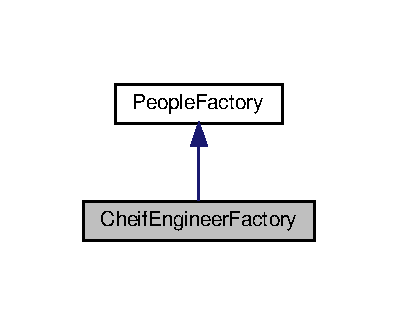
\includegraphics[width=191pt]{classCheifEngineerFactory__inherit__graph}
\end{center}
\end{figure}


Collaboration diagram for Cheif\+Engineer\+Factory\+:\nopagebreak
\begin{figure}[H]
\begin{center}
\leavevmode
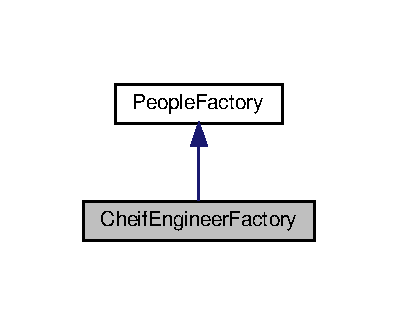
\includegraphics[width=191pt]{classCheifEngineerFactory__coll__graph}
\end{center}
\end{figure}
\subsection*{Public Member Functions}
\begin{DoxyCompactItemize}
\item 
\hyperlink{classCheifEngineerFactory_aa3b45f6d06a640bc77086f58ccffe650}{Cheif\+Engineer\+Factory} ()
\item 
\hyperlink{classCheifEngineerFactory_ac6c5623874406c88cd34badb6294c998}{$\sim$\+Cheif\+Engineer\+Factory} ()
\item 
\hyperlink{classPeople}{People} $\ast$ \hyperlink{classCheifEngineerFactory_a3a593a010ee16ec52670601e0c5c72d5}{create} ()
\end{DoxyCompactItemize}


\subsection{Detailed Description}
Chief \hyperlink{classEngineer}{Engineer} Factory. 

\subsection{Constructor \& Destructor Documentation}
\mbox{\Hypertarget{classCheifEngineerFactory_aa3b45f6d06a640bc77086f58ccffe650}\label{classCheifEngineerFactory_aa3b45f6d06a640bc77086f58ccffe650}} 
\index{Cheif\+Engineer\+Factory@{Cheif\+Engineer\+Factory}!Cheif\+Engineer\+Factory@{Cheif\+Engineer\+Factory}}
\index{Cheif\+Engineer\+Factory@{Cheif\+Engineer\+Factory}!Cheif\+Engineer\+Factory@{Cheif\+Engineer\+Factory}}
\subsubsection{\texorpdfstring{Cheif\+Engineer\+Factory()}{CheifEngineerFactory()}}
{\footnotesize\ttfamily Cheif\+Engineer\+Factory\+::\+Cheif\+Engineer\+Factory (\begin{DoxyParamCaption}{ }\end{DoxyParamCaption})\hspace{0.3cm}{\ttfamily [inline]}}

Default constructor \mbox{\Hypertarget{classCheifEngineerFactory_ac6c5623874406c88cd34badb6294c998}\label{classCheifEngineerFactory_ac6c5623874406c88cd34badb6294c998}} 
\index{Cheif\+Engineer\+Factory@{Cheif\+Engineer\+Factory}!````~Cheif\+Engineer\+Factory@{$\sim$\+Cheif\+Engineer\+Factory}}
\index{````~Cheif\+Engineer\+Factory@{$\sim$\+Cheif\+Engineer\+Factory}!Cheif\+Engineer\+Factory@{Cheif\+Engineer\+Factory}}
\subsubsection{\texorpdfstring{$\sim$\+Cheif\+Engineer\+Factory()}{~CheifEngineerFactory()}}
{\footnotesize\ttfamily Cheif\+Engineer\+Factory\+::$\sim$\+Cheif\+Engineer\+Factory (\begin{DoxyParamCaption}{ }\end{DoxyParamCaption})\hspace{0.3cm}{\ttfamily [inline]}}

Default destructor 

\subsection{Member Function Documentation}
\mbox{\Hypertarget{classCheifEngineerFactory_a3a593a010ee16ec52670601e0c5c72d5}\label{classCheifEngineerFactory_a3a593a010ee16ec52670601e0c5c72d5}} 
\index{Cheif\+Engineer\+Factory@{Cheif\+Engineer\+Factory}!create@{create}}
\index{create@{create}!Cheif\+Engineer\+Factory@{Cheif\+Engineer\+Factory}}
\subsubsection{\texorpdfstring{create()}{create()}}
{\footnotesize\ttfamily \hyperlink{classPeople}{People}$\ast$ Cheif\+Engineer\+Factory\+::create (\begin{DoxyParamCaption}{ }\end{DoxyParamCaption})\hspace{0.3cm}{\ttfamily [inline]}, {\ttfamily [virtual]}}

creates \hyperlink{classChiefEngineer}{Chief\+Engineer} 

Implements \hyperlink{classPeopleFactory}{People\+Factory}.



The documentation for this class was generated from the following file\+:\begin{DoxyCompactItemize}
\item 
Chief\+Engineer\+Factory.\+h\end{DoxyCompactItemize}

\hypertarget{classChiefEngineer}{}\section{Chief\+Engineer Class Reference}
\label{classChiefEngineer}\index{Chief\+Engineer@{Chief\+Engineer}}


Chief \hyperlink{classEngineer}{Engineer} class.  




{\ttfamily \#include $<$Chief\+Engineer.\+h$>$}



Inheritance diagram for Chief\+Engineer\+:\nopagebreak
\begin{figure}[H]
\begin{center}
\leavevmode
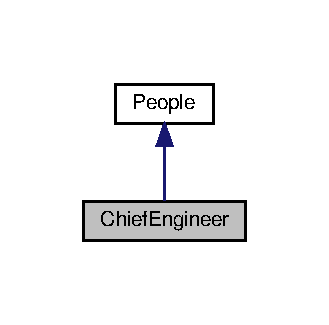
\includegraphics[width=158pt]{classChiefEngineer__inherit__graph}
\end{center}
\end{figure}


Collaboration diagram for Chief\+Engineer\+:\nopagebreak
\begin{figure}[H]
\begin{center}
\leavevmode
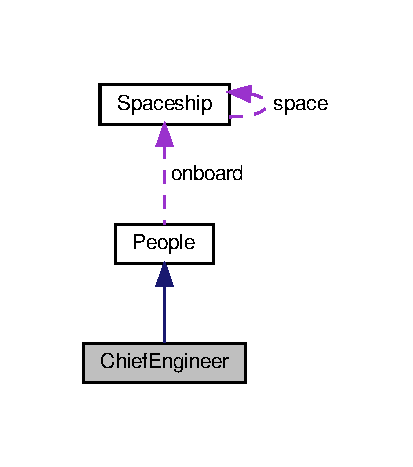
\includegraphics[width=198pt]{classChiefEngineer__coll__graph}
\end{center}
\end{figure}
\subsection*{Public Member Functions}
\begin{DoxyCompactItemize}
\item 
\hyperlink{classChiefEngineer_a4bd0e5f9075ad0ac1a15047c152fe2cb}{Chief\+Engineer} ()
\item 
\hyperlink{classChiefEngineer_aa647c8d8f2d872dc3838211725fd05db}{$\sim$\+Chief\+Engineer} ()
\item 
void \hyperlink{classChiefEngineer_a7170ae93d7eadc1a68bc86c25a9be0db}{recieve\+Spaceship\+Error} (string)
\item 
void \hyperlink{classChiefEngineer_afe5a4677f7651fff2926c0583875a666}{send\+Error\+Message} (string)
\item 
string \hyperlink{classChiefEngineer_abd3df4d2f94acff4c659f9e428ad1789}{get\+Type} ()
\end{DoxyCompactItemize}
\subsection*{Additional Inherited Members}


\subsection{Detailed Description}
Chief \hyperlink{classEngineer}{Engineer} class. 

\subsection{Constructor \& Destructor Documentation}
\mbox{\Hypertarget{classChiefEngineer_a4bd0e5f9075ad0ac1a15047c152fe2cb}\label{classChiefEngineer_a4bd0e5f9075ad0ac1a15047c152fe2cb}} 
\index{Chief\+Engineer@{Chief\+Engineer}!Chief\+Engineer@{Chief\+Engineer}}
\index{Chief\+Engineer@{Chief\+Engineer}!Chief\+Engineer@{Chief\+Engineer}}
\subsubsection{\texorpdfstring{Chief\+Engineer()}{ChiefEngineer()}}
{\footnotesize\ttfamily Chief\+Engineer\+::\+Chief\+Engineer (\begin{DoxyParamCaption}{ }\end{DoxyParamCaption})\hspace{0.3cm}{\ttfamily [inline]}}

Default constructor \mbox{\Hypertarget{classChiefEngineer_aa647c8d8f2d872dc3838211725fd05db}\label{classChiefEngineer_aa647c8d8f2d872dc3838211725fd05db}} 
\index{Chief\+Engineer@{Chief\+Engineer}!````~Chief\+Engineer@{$\sim$\+Chief\+Engineer}}
\index{````~Chief\+Engineer@{$\sim$\+Chief\+Engineer}!Chief\+Engineer@{Chief\+Engineer}}
\subsubsection{\texorpdfstring{$\sim$\+Chief\+Engineer()}{~ChiefEngineer()}}
{\footnotesize\ttfamily Chief\+Engineer\+::$\sim$\+Chief\+Engineer (\begin{DoxyParamCaption}{ }\end{DoxyParamCaption})\hspace{0.3cm}{\ttfamily [inline]}}

Default destructor 

\subsection{Member Function Documentation}
\mbox{\Hypertarget{classChiefEngineer_abd3df4d2f94acff4c659f9e428ad1789}\label{classChiefEngineer_abd3df4d2f94acff4c659f9e428ad1789}} 
\index{Chief\+Engineer@{Chief\+Engineer}!get\+Type@{get\+Type}}
\index{get\+Type@{get\+Type}!Chief\+Engineer@{Chief\+Engineer}}
\subsubsection{\texorpdfstring{get\+Type()}{getType()}}
{\footnotesize\ttfamily string Chief\+Engineer\+::get\+Type (\begin{DoxyParamCaption}{ }\end{DoxyParamCaption})\hspace{0.3cm}{\ttfamily [inline]}, {\ttfamily [virtual]}}

Getting type of the person 

Implements \hyperlink{classPeople_af60dd882d60cddf63f9b95815ce551a8}{People}.

\mbox{\Hypertarget{classChiefEngineer_a7170ae93d7eadc1a68bc86c25a9be0db}\label{classChiefEngineer_a7170ae93d7eadc1a68bc86c25a9be0db}} 
\index{Chief\+Engineer@{Chief\+Engineer}!recieve\+Spaceship\+Error@{recieve\+Spaceship\+Error}}
\index{recieve\+Spaceship\+Error@{recieve\+Spaceship\+Error}!Chief\+Engineer@{Chief\+Engineer}}
\subsubsection{\texorpdfstring{recieve\+Spaceship\+Error()}{recieveSpaceshipError()}}
{\footnotesize\ttfamily void Chief\+Engineer\+::recieve\+Spaceship\+Error (\begin{DoxyParamCaption}\item[{string}]{message }\end{DoxyParamCaption})\hspace{0.3cm}{\ttfamily [virtual]}}

Receive an error from the spaceship 
\begin{DoxyParams}{Parameters}
{\em message} & -\/ The message being transmitted \\
\hline
\end{DoxyParams}


Implements \hyperlink{classPeople_a0685df78be631783138865e03cc7c85d}{People}.

\mbox{\Hypertarget{classChiefEngineer_afe5a4677f7651fff2926c0583875a666}\label{classChiefEngineer_afe5a4677f7651fff2926c0583875a666}} 
\index{Chief\+Engineer@{Chief\+Engineer}!send\+Error\+Message@{send\+Error\+Message}}
\index{send\+Error\+Message@{send\+Error\+Message}!Chief\+Engineer@{Chief\+Engineer}}
\subsubsection{\texorpdfstring{send\+Error\+Message()}{sendErrorMessage()}}
{\footnotesize\ttfamily void Chief\+Engineer\+::send\+Error\+Message (\begin{DoxyParamCaption}\item[{string}]{message }\end{DoxyParamCaption})\hspace{0.3cm}{\ttfamily [virtual]}}

Send an error to the spaceship 
\begin{DoxyParams}{Parameters}
{\em message} & -\/ the message to transmit \\
\hline
\end{DoxyParams}


Implements \hyperlink{classPeople_a572a35170f61d1848eb04b65baafb057}{People}.



The documentation for this class was generated from the following files\+:\begin{DoxyCompactItemize}
\item 
Chief\+Engineer.\+h\item 
Chief\+Engineer.\+cpp\end{DoxyCompactItemize}

\hypertarget{classCommand}{}\section{Command Class Reference}
\label{classCommand}\index{Command@{Command}}


\hyperlink{classPlanet}{Planet} class.  




{\ttfamily \#include $<$Command.\+h$>$}



Inheritance diagram for Command\+:\nopagebreak
\begin{figure}[H]
\begin{center}
\leavevmode
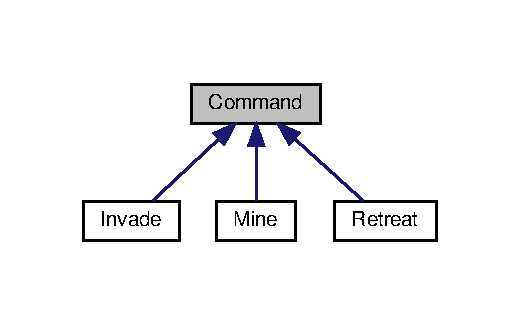
\includegraphics[width=250pt]{classCommand__inherit__graph}
\end{center}
\end{figure}
\subsection*{Public Member Functions}
\begin{DoxyCompactItemize}
\item 
\hyperlink{classCommand_a18df2d81039392daeb0b78c346a70537}{Command} ()
\item 
virtual void \hyperlink{classCommand_a6fd7d9bd8df8bfc881e4d6c7cd1878b7}{execute} ()=0
\item 
\hyperlink{classCommand_ab552bb3a07fdd1acbfd8ea76e69b2278}{$\sim$\+Command} ()
\end{DoxyCompactItemize}


\subsection{Detailed Description}
\hyperlink{classPlanet}{Planet} class. 

\subsection{Constructor \& Destructor Documentation}
\mbox{\Hypertarget{classCommand_a18df2d81039392daeb0b78c346a70537}\label{classCommand_a18df2d81039392daeb0b78c346a70537}} 
\index{Command@{Command}!Command@{Command}}
\index{Command@{Command}!Command@{Command}}
\subsubsection{\texorpdfstring{Command()}{Command()}}
{\footnotesize\ttfamily Command\+::\+Command (\begin{DoxyParamCaption}{ }\end{DoxyParamCaption})\hspace{0.3cm}{\ttfamily [inline]}}

default constructor \mbox{\Hypertarget{classCommand_ab552bb3a07fdd1acbfd8ea76e69b2278}\label{classCommand_ab552bb3a07fdd1acbfd8ea76e69b2278}} 
\index{Command@{Command}!````~Command@{$\sim$\+Command}}
\index{````~Command@{$\sim$\+Command}!Command@{Command}}
\subsubsection{\texorpdfstring{$\sim$\+Command()}{~Command()}}
{\footnotesize\ttfamily Command\+::$\sim$\+Command (\begin{DoxyParamCaption}{ }\end{DoxyParamCaption})\hspace{0.3cm}{\ttfamily [inline]}}

Default Destructor 

\subsection{Member Function Documentation}
\mbox{\Hypertarget{classCommand_a6fd7d9bd8df8bfc881e4d6c7cd1878b7}\label{classCommand_a6fd7d9bd8df8bfc881e4d6c7cd1878b7}} 
\index{Command@{Command}!execute@{execute}}
\index{execute@{execute}!Command@{Command}}
\subsubsection{\texorpdfstring{execute()}{execute()}}
{\footnotesize\ttfamily virtual void Command\+::execute (\begin{DoxyParamCaption}{ }\end{DoxyParamCaption})\hspace{0.3cm}{\ttfamily [pure virtual]}}

Pure Virtual Execute Function That will be implemented by sub classes 

Implemented in \hyperlink{classInvade_a111ebe8b6c5a3646b697ca906c815b35}{Invade}, \hyperlink{classMine_a2cfa55d098ec47369eed81226d82da25}{Mine}, and \hyperlink{classRetreat_a18fe7bf00ed623de02de5764b9607f5f}{Retreat}.



The documentation for this class was generated from the following file\+:\begin{DoxyCompactItemize}
\item 
Command.\+h\end{DoxyCompactItemize}

\hypertarget{classCommanderOfTheFleet}{}\section{Commander\+Of\+The\+Fleet Class Reference}
\label{classCommanderOfTheFleet}\index{Commander\+Of\+The\+Fleet@{Commander\+Of\+The\+Fleet}}


Commander of the fleet class. A singleton.  




{\ttfamily \#include $<$Commander\+Of\+The\+Fleet.\+h$>$}



Inheritance diagram for Commander\+Of\+The\+Fleet\+:\nopagebreak
\begin{figure}[H]
\begin{center}
\leavevmode
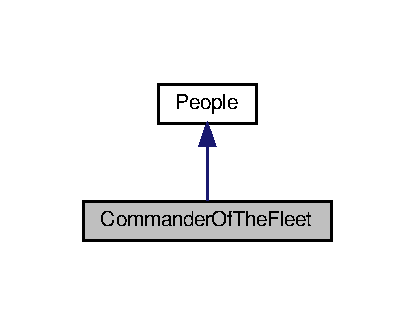
\includegraphics[width=199pt]{classCommanderOfTheFleet__inherit__graph}
\end{center}
\end{figure}


Collaboration diagram for Commander\+Of\+The\+Fleet\+:\nopagebreak
\begin{figure}[H]
\begin{center}
\leavevmode
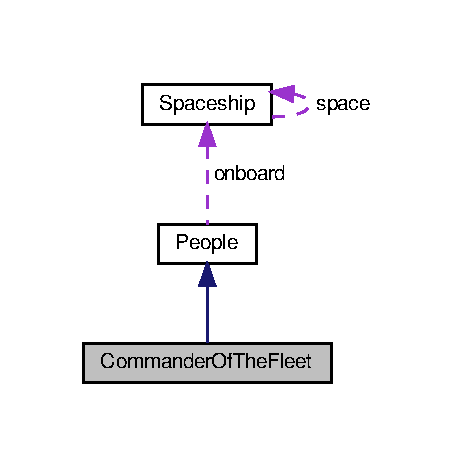
\includegraphics[width=219pt]{classCommanderOfTheFleet__coll__graph}
\end{center}
\end{figure}
\subsection*{Public Member Functions}
\begin{DoxyCompactItemize}
\item 
void \hyperlink{classCommanderOfTheFleet_a13e91b9342df067b375f7ef2b929c0d5}{recieve\+Spaceship\+Error} (string)
\item 
void \hyperlink{classCommanderOfTheFleet_a39cfd5c0016355543515e919791d7984}{send\+Error\+Message} (string)
\item 
string \hyperlink{classCommanderOfTheFleet_a6e025eb090e0e231ffa72e5e6a9f7ce0}{get\+Type} ()
\item 
void \hyperlink{classCommanderOfTheFleet_a083604612b705c159fdd16dff0d2d396}{do\+Command} (string, \hyperlink{classSpaceship}{Spaceship} $\ast$)
\end{DoxyCompactItemize}
\subsection*{Static Public Member Functions}
\begin{DoxyCompactItemize}
\item 
static \hyperlink{classCommanderOfTheFleet}{Commander\+Of\+The\+Fleet} $\ast$ \hyperlink{classCommanderOfTheFleet_a19e2583c1a60a01f5530b0f97fbcbca5}{instance} ()
\end{DoxyCompactItemize}
\subsection*{Protected Member Functions}
\begin{DoxyCompactItemize}
\item 
\hyperlink{classCommanderOfTheFleet_a8b61f0fbb16d5e8cbeda75d931b271c6}{Commander\+Of\+The\+Fleet} ()
\item 
virtual \hyperlink{classCommanderOfTheFleet_a63fcb504fd7d5dc035814bc137875cd2}{$\sim$\+Commander\+Of\+The\+Fleet} ()
\item 
\hyperlink{classCommanderOfTheFleet_a83cb8584c7f588f533bc33ed0168188b}{Commander\+Of\+The\+Fleet} (const \hyperlink{classCommanderOfTheFleet}{Commander\+Of\+The\+Fleet} \&)
\item 
\hyperlink{classCommanderOfTheFleet}{Commander\+Of\+The\+Fleet} \& \hyperlink{classCommanderOfTheFleet_aaa476181b99052293306fcfe57dfd642}{operator=} (const \hyperlink{classCommanderOfTheFleet}{Commander\+Of\+The\+Fleet} \&)
\end{DoxyCompactItemize}
\subsection*{Additional Inherited Members}


\subsection{Detailed Description}
Commander of the fleet class. A singleton. 

\subsection{Constructor \& Destructor Documentation}
\mbox{\Hypertarget{classCommanderOfTheFleet_a8b61f0fbb16d5e8cbeda75d931b271c6}\label{classCommanderOfTheFleet_a8b61f0fbb16d5e8cbeda75d931b271c6}} 
\index{Commander\+Of\+The\+Fleet@{Commander\+Of\+The\+Fleet}!Commander\+Of\+The\+Fleet@{Commander\+Of\+The\+Fleet}}
\index{Commander\+Of\+The\+Fleet@{Commander\+Of\+The\+Fleet}!Commander\+Of\+The\+Fleet@{Commander\+Of\+The\+Fleet}}
\subsubsection{\texorpdfstring{Commander\+Of\+The\+Fleet()}{CommanderOfTheFleet()}\hspace{0.1cm}{\footnotesize\ttfamily [1/2]}}
{\footnotesize\ttfamily Commander\+Of\+The\+Fleet\+::\+Commander\+Of\+The\+Fleet (\begin{DoxyParamCaption}{ }\end{DoxyParamCaption})\hspace{0.3cm}{\ttfamily [protected]}}

Default constructor \mbox{\Hypertarget{classCommanderOfTheFleet_a63fcb504fd7d5dc035814bc137875cd2}\label{classCommanderOfTheFleet_a63fcb504fd7d5dc035814bc137875cd2}} 
\index{Commander\+Of\+The\+Fleet@{Commander\+Of\+The\+Fleet}!````~Commander\+Of\+The\+Fleet@{$\sim$\+Commander\+Of\+The\+Fleet}}
\index{````~Commander\+Of\+The\+Fleet@{$\sim$\+Commander\+Of\+The\+Fleet}!Commander\+Of\+The\+Fleet@{Commander\+Of\+The\+Fleet}}
\subsubsection{\texorpdfstring{$\sim$\+Commander\+Of\+The\+Fleet()}{~CommanderOfTheFleet()}}
{\footnotesize\ttfamily Commander\+Of\+The\+Fleet\+::$\sim$\+Commander\+Of\+The\+Fleet (\begin{DoxyParamCaption}{ }\end{DoxyParamCaption})\hspace{0.3cm}{\ttfamily [protected]}, {\ttfamily [virtual]}}

Virtual default destructor \mbox{\Hypertarget{classCommanderOfTheFleet_a83cb8584c7f588f533bc33ed0168188b}\label{classCommanderOfTheFleet_a83cb8584c7f588f533bc33ed0168188b}} 
\index{Commander\+Of\+The\+Fleet@{Commander\+Of\+The\+Fleet}!Commander\+Of\+The\+Fleet@{Commander\+Of\+The\+Fleet}}
\index{Commander\+Of\+The\+Fleet@{Commander\+Of\+The\+Fleet}!Commander\+Of\+The\+Fleet@{Commander\+Of\+The\+Fleet}}
\subsubsection{\texorpdfstring{Commander\+Of\+The\+Fleet()}{CommanderOfTheFleet()}\hspace{0.1cm}{\footnotesize\ttfamily [2/2]}}
{\footnotesize\ttfamily Commander\+Of\+The\+Fleet\+::\+Commander\+Of\+The\+Fleet (\begin{DoxyParamCaption}\item[{const \hyperlink{classCommanderOfTheFleet}{Commander\+Of\+The\+Fleet} \&}]{s }\end{DoxyParamCaption})\hspace{0.3cm}{\ttfamily [protected]}}

Parameterised constructor. In order to prevent copies being created 

\subsection{Member Function Documentation}
\mbox{\Hypertarget{classCommanderOfTheFleet_a083604612b705c159fdd16dff0d2d396}\label{classCommanderOfTheFleet_a083604612b705c159fdd16dff0d2d396}} 
\index{Commander\+Of\+The\+Fleet@{Commander\+Of\+The\+Fleet}!do\+Command@{do\+Command}}
\index{do\+Command@{do\+Command}!Commander\+Of\+The\+Fleet@{Commander\+Of\+The\+Fleet}}
\subsubsection{\texorpdfstring{do\+Command()}{doCommand()}}
{\footnotesize\ttfamily void Commander\+Of\+The\+Fleet\+::do\+Command (\begin{DoxyParamCaption}\item[{string}]{type,  }\item[{\hyperlink{classSpaceship}{Spaceship} $\ast$}]{s }\end{DoxyParamCaption})}

Execute a command 
\begin{DoxyParams}{Parameters}
{\em type} & -\/ the command type \\
\hline
\end{DoxyParams}
\mbox{\Hypertarget{classCommanderOfTheFleet_a6e025eb090e0e231ffa72e5e6a9f7ce0}\label{classCommanderOfTheFleet_a6e025eb090e0e231ffa72e5e6a9f7ce0}} 
\index{Commander\+Of\+The\+Fleet@{Commander\+Of\+The\+Fleet}!get\+Type@{get\+Type}}
\index{get\+Type@{get\+Type}!Commander\+Of\+The\+Fleet@{Commander\+Of\+The\+Fleet}}
\subsubsection{\texorpdfstring{get\+Type()}{getType()}}
{\footnotesize\ttfamily string Commander\+Of\+The\+Fleet\+::get\+Type (\begin{DoxyParamCaption}{ }\end{DoxyParamCaption})\hspace{0.3cm}{\ttfamily [inline]}, {\ttfamily [virtual]}}

get type of person 

Implements \hyperlink{classPeople_af60dd882d60cddf63f9b95815ce551a8}{People}.

\mbox{\Hypertarget{classCommanderOfTheFleet_a19e2583c1a60a01f5530b0f97fbcbca5}\label{classCommanderOfTheFleet_a19e2583c1a60a01f5530b0f97fbcbca5}} 
\index{Commander\+Of\+The\+Fleet@{Commander\+Of\+The\+Fleet}!instance@{instance}}
\index{instance@{instance}!Commander\+Of\+The\+Fleet@{Commander\+Of\+The\+Fleet}}
\subsubsection{\texorpdfstring{instance()}{instance()}}
{\footnotesize\ttfamily \hyperlink{classCommanderOfTheFleet}{Commander\+Of\+The\+Fleet} $\ast$ Commander\+Of\+The\+Fleet\+::instance (\begin{DoxyParamCaption}{ }\end{DoxyParamCaption})\hspace{0.3cm}{\ttfamily [static]}}

Creates or returns a single instance of the commander \begin{DoxyReturn}{Returns}
Commander\+Of\+The\+Fleet$\ast$ 
\end{DoxyReturn}
\mbox{\Hypertarget{classCommanderOfTheFleet_aaa476181b99052293306fcfe57dfd642}\label{classCommanderOfTheFleet_aaa476181b99052293306fcfe57dfd642}} 
\index{Commander\+Of\+The\+Fleet@{Commander\+Of\+The\+Fleet}!operator=@{operator=}}
\index{operator=@{operator=}!Commander\+Of\+The\+Fleet@{Commander\+Of\+The\+Fleet}}
\subsubsection{\texorpdfstring{operator=()}{operator=()}}
{\footnotesize\ttfamily \hyperlink{classCommanderOfTheFleet}{Commander\+Of\+The\+Fleet} \& Commander\+Of\+The\+Fleet\+::operator= (\begin{DoxyParamCaption}\item[{const \hyperlink{classCommanderOfTheFleet}{Commander\+Of\+The\+Fleet} \&}]{s }\end{DoxyParamCaption})\hspace{0.3cm}{\ttfamily [protected]}}

Overridden = operator. Protects the singleton 
\begin{DoxyParams}{Parameters}
{\em Commander\+Of\+The\+Fleet\&} & -\/ a reference to the commander \\
\hline
\end{DoxyParams}
\begin{DoxyReturn}{Returns}
\hyperlink{classCommanderOfTheFleet}{Commander\+Of\+The\+Fleet}\& 
\end{DoxyReturn}
\mbox{\Hypertarget{classCommanderOfTheFleet_a13e91b9342df067b375f7ef2b929c0d5}\label{classCommanderOfTheFleet_a13e91b9342df067b375f7ef2b929c0d5}} 
\index{Commander\+Of\+The\+Fleet@{Commander\+Of\+The\+Fleet}!recieve\+Spaceship\+Error@{recieve\+Spaceship\+Error}}
\index{recieve\+Spaceship\+Error@{recieve\+Spaceship\+Error}!Commander\+Of\+The\+Fleet@{Commander\+Of\+The\+Fleet}}
\subsubsection{\texorpdfstring{recieve\+Spaceship\+Error()}{recieveSpaceshipError()}}
{\footnotesize\ttfamily void Commander\+Of\+The\+Fleet\+::recieve\+Spaceship\+Error (\begin{DoxyParamCaption}\item[{string}]{message }\end{DoxyParamCaption})\hspace{0.3cm}{\ttfamily [virtual]}}

Receive an error from the spaceship 
\begin{DoxyParams}{Parameters}
{\em message} & -\/ the message recieved \\
\hline
\end{DoxyParams}


Implements \hyperlink{classPeople_a0685df78be631783138865e03cc7c85d}{People}.

\mbox{\Hypertarget{classCommanderOfTheFleet_a39cfd5c0016355543515e919791d7984}\label{classCommanderOfTheFleet_a39cfd5c0016355543515e919791d7984}} 
\index{Commander\+Of\+The\+Fleet@{Commander\+Of\+The\+Fleet}!send\+Error\+Message@{send\+Error\+Message}}
\index{send\+Error\+Message@{send\+Error\+Message}!Commander\+Of\+The\+Fleet@{Commander\+Of\+The\+Fleet}}
\subsubsection{\texorpdfstring{send\+Error\+Message()}{sendErrorMessage()}}
{\footnotesize\ttfamily void Commander\+Of\+The\+Fleet\+::send\+Error\+Message (\begin{DoxyParamCaption}\item[{string}]{message }\end{DoxyParamCaption})\hspace{0.3cm}{\ttfamily [virtual]}}

Send an error to the spaceship 
\begin{DoxyParams}{Parameters}
{\em message} & -\/ The message to be sent \\
\hline
\end{DoxyParams}


Implements \hyperlink{classPeople_a572a35170f61d1848eb04b65baafb057}{People}.



The documentation for this class was generated from the following files\+:\begin{DoxyCompactItemize}
\item 
Commander\+Of\+The\+Fleet.\+h\item 
Commander\+Of\+The\+Fleet.\+cpp\end{DoxyCompactItemize}

\hypertarget{classCommanderOfTheFleetFactory}{}\section{Commander\+Of\+The\+Fleet\+Factory Class Reference}
\label{classCommanderOfTheFleetFactory}\index{Commander\+Of\+The\+Fleet\+Factory@{Commander\+Of\+The\+Fleet\+Factory}}


Commander of the fleet factory class.  




{\ttfamily \#include $<$Commander\+Of\+The\+Fleet\+Factory.\+h$>$}



Inheritance diagram for Commander\+Of\+The\+Fleet\+Factory\+:\nopagebreak
\begin{figure}[H]
\begin{center}
\leavevmode
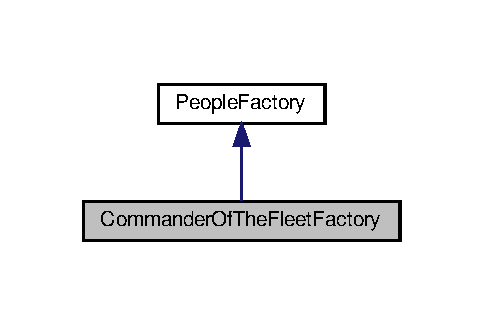
\includegraphics[width=232pt]{classCommanderOfTheFleetFactory__inherit__graph}
\end{center}
\end{figure}


Collaboration diagram for Commander\+Of\+The\+Fleet\+Factory\+:\nopagebreak
\begin{figure}[H]
\begin{center}
\leavevmode
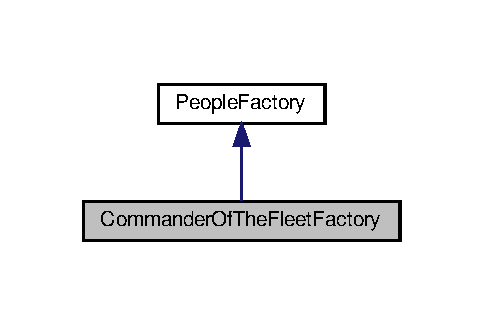
\includegraphics[width=232pt]{classCommanderOfTheFleetFactory__coll__graph}
\end{center}
\end{figure}
\subsection*{Public Member Functions}
\begin{DoxyCompactItemize}
\item 
\hyperlink{classCommanderOfTheFleetFactory_a8a5df50232cc48a885ba2a05928a8301}{Commander\+Of\+The\+Fleet\+Factory} ()
\item 
\hyperlink{classCommanderOfTheFleetFactory_ad6a8e81a67057ce5d65c47289cd7b4f4}{$\sim$\+Commander\+Of\+The\+Fleet\+Factory} ()
\item 
\hyperlink{classPeople}{People} $\ast$ \hyperlink{classCommanderOfTheFleetFactory_aabbbbcb6c52f23e008b186e59aa5c84b}{create} ()
\end{DoxyCompactItemize}


\subsection{Detailed Description}
Commander of the fleet factory class. 

\subsection{Constructor \& Destructor Documentation}
\mbox{\Hypertarget{classCommanderOfTheFleetFactory_a8a5df50232cc48a885ba2a05928a8301}\label{classCommanderOfTheFleetFactory_a8a5df50232cc48a885ba2a05928a8301}} 
\index{Commander\+Of\+The\+Fleet\+Factory@{Commander\+Of\+The\+Fleet\+Factory}!Commander\+Of\+The\+Fleet\+Factory@{Commander\+Of\+The\+Fleet\+Factory}}
\index{Commander\+Of\+The\+Fleet\+Factory@{Commander\+Of\+The\+Fleet\+Factory}!Commander\+Of\+The\+Fleet\+Factory@{Commander\+Of\+The\+Fleet\+Factory}}
\subsubsection{\texorpdfstring{Commander\+Of\+The\+Fleet\+Factory()}{CommanderOfTheFleetFactory()}}
{\footnotesize\ttfamily Commander\+Of\+The\+Fleet\+Factory\+::\+Commander\+Of\+The\+Fleet\+Factory (\begin{DoxyParamCaption}{ }\end{DoxyParamCaption})\hspace{0.3cm}{\ttfamily [inline]}}

Default constructor \mbox{\Hypertarget{classCommanderOfTheFleetFactory_ad6a8e81a67057ce5d65c47289cd7b4f4}\label{classCommanderOfTheFleetFactory_ad6a8e81a67057ce5d65c47289cd7b4f4}} 
\index{Commander\+Of\+The\+Fleet\+Factory@{Commander\+Of\+The\+Fleet\+Factory}!````~Commander\+Of\+The\+Fleet\+Factory@{$\sim$\+Commander\+Of\+The\+Fleet\+Factory}}
\index{````~Commander\+Of\+The\+Fleet\+Factory@{$\sim$\+Commander\+Of\+The\+Fleet\+Factory}!Commander\+Of\+The\+Fleet\+Factory@{Commander\+Of\+The\+Fleet\+Factory}}
\subsubsection{\texorpdfstring{$\sim$\+Commander\+Of\+The\+Fleet\+Factory()}{~CommanderOfTheFleetFactory()}}
{\footnotesize\ttfamily Commander\+Of\+The\+Fleet\+Factory\+::$\sim$\+Commander\+Of\+The\+Fleet\+Factory (\begin{DoxyParamCaption}{ }\end{DoxyParamCaption})\hspace{0.3cm}{\ttfamily [inline]}}

Default desctructor 

\subsection{Member Function Documentation}
\mbox{\Hypertarget{classCommanderOfTheFleetFactory_aabbbbcb6c52f23e008b186e59aa5c84b}\label{classCommanderOfTheFleetFactory_aabbbbcb6c52f23e008b186e59aa5c84b}} 
\index{Commander\+Of\+The\+Fleet\+Factory@{Commander\+Of\+The\+Fleet\+Factory}!create@{create}}
\index{create@{create}!Commander\+Of\+The\+Fleet\+Factory@{Commander\+Of\+The\+Fleet\+Factory}}
\subsubsection{\texorpdfstring{create()}{create()}}
{\footnotesize\ttfamily \hyperlink{classPeople}{People}$\ast$ Commander\+Of\+The\+Fleet\+Factory\+::create (\begin{DoxyParamCaption}{ }\end{DoxyParamCaption})\hspace{0.3cm}{\ttfamily [inline]}, {\ttfamily [virtual]}}

creates \hyperlink{classCommanderOfTheFleet}{Commander\+Of\+The\+Fleet} 

Implements \hyperlink{classPeopleFactory}{People\+Factory}.



The documentation for this class was generated from the following file\+:\begin{DoxyCompactItemize}
\item 
Commander\+Of\+The\+Fleet\+Factory.\+h\end{DoxyCompactItemize}

\hypertarget{classComms}{}\section{Comms Class Reference}
\label{classComms}\index{Comms@{Comms}}


\hyperlink{classComms}{Comms} class.  




{\ttfamily \#include $<$Comms.\+h$>$}



Inheritance diagram for Comms\+:
% FIG 0


Collaboration diagram for Comms\+:
% FIG 1
\subsection*{Public Member Functions}
\begin{DoxyCompactItemize}
\item 
\hyperlink{classComms_aa3878221ed907d6d6841ee77741c1f49}{Comms} ()
\item 
\hyperlink{classComms_ad18d3a80a82d18d27b0de3b551e4f5fc}{$\sim$\+Comms} ()
\item 
void \hyperlink{classComms_a1aed1c01a813afd55309fdc59d2871bf}{recieve\+Spaceship\+Error} (string)
\item 
void \hyperlink{classComms_a23c37f6d10f06c7cfe25c4dc7d62fa12}{send\+Error\+Message} (string)
\end{DoxyCompactItemize}
\subsection*{Additional Inherited Members}


\subsection{Detailed Description}
\hyperlink{classComms}{Comms} class. 

\subsection{Constructor \& Destructor Documentation}
\mbox{\Hypertarget{classComms_aa3878221ed907d6d6841ee77741c1f49}\label{classComms_aa3878221ed907d6d6841ee77741c1f49}} 
\index{Comms@{Comms}!Comms@{Comms}}
\index{Comms@{Comms}!Comms@{Comms}}
\subsubsection{\texorpdfstring{Comms()}{Comms()}}
{\footnotesize\ttfamily Comms\+::\+Comms (\begin{DoxyParamCaption}{ }\end{DoxyParamCaption})\hspace{0.3cm}{\ttfamily [inline]}}

Default constructor \mbox{\Hypertarget{classComms_ad18d3a80a82d18d27b0de3b551e4f5fc}\label{classComms_ad18d3a80a82d18d27b0de3b551e4f5fc}} 
\index{Comms@{Comms}!````~Comms@{$\sim$\+Comms}}
\index{````~Comms@{$\sim$\+Comms}!Comms@{Comms}}
\subsubsection{\texorpdfstring{$\sim$\+Comms()}{~Comms()}}
{\footnotesize\ttfamily Comms\+::$\sim$\+Comms (\begin{DoxyParamCaption}{ }\end{DoxyParamCaption})\hspace{0.3cm}{\ttfamily [inline]}}

Default desctructor 

\subsection{Member Function Documentation}
\mbox{\Hypertarget{classComms_a1aed1c01a813afd55309fdc59d2871bf}\label{classComms_a1aed1c01a813afd55309fdc59d2871bf}} 
\index{Comms@{Comms}!recieve\+Spaceship\+Error@{recieve\+Spaceship\+Error}}
\index{recieve\+Spaceship\+Error@{recieve\+Spaceship\+Error}!Comms@{Comms}}
\subsubsection{\texorpdfstring{recieve\+Spaceship\+Error()}{recieveSpaceshipError()}}
{\footnotesize\ttfamily void Comms\+::recieve\+Spaceship\+Error (\begin{DoxyParamCaption}\item[{string}]{message }\end{DoxyParamCaption})\hspace{0.3cm}{\ttfamily [virtual]}}

Recieve an error from the spaceship 
\begin{DoxyParams}{Parameters}
{\em message} & -\/ the error message being received \\
\hline
\end{DoxyParams}


Implements \hyperlink{classPeople_a0685df78be631783138865e03cc7c85d}{People}.

\mbox{\Hypertarget{classComms_a23c37f6d10f06c7cfe25c4dc7d62fa12}\label{classComms_a23c37f6d10f06c7cfe25c4dc7d62fa12}} 
\index{Comms@{Comms}!send\+Error\+Message@{send\+Error\+Message}}
\index{send\+Error\+Message@{send\+Error\+Message}!Comms@{Comms}}
\subsubsection{\texorpdfstring{send\+Error\+Message()}{sendErrorMessage()}}
{\footnotesize\ttfamily void Comms\+::send\+Error\+Message (\begin{DoxyParamCaption}\item[{string}]{message }\end{DoxyParamCaption})\hspace{0.3cm}{\ttfamily [virtual]}}

Send an error to the spaceship 
\begin{DoxyParams}{Parameters}
{\em message} & -\/ the error message being sent \\
\hline
\end{DoxyParams}


Implements \hyperlink{classPeople_a572a35170f61d1848eb04b65baafb057}{People}.



The documentation for this class was generated from the following files\+:\begin{DoxyCompactItemize}
\item 
Comms.\+h\item 
Comms.\+cpp\end{DoxyCompactItemize}

\hypertarget{classCommsFactory}{}\section{Comms\+Factory Class Reference}
\label{classCommsFactory}\index{Comms\+Factory@{Comms\+Factory}}


\hyperlink{classCommsFactory}{Comms\+Factory} class.  




{\ttfamily \#include $<$Comms\+Factory.\+h$>$}



Inheritance diagram for Comms\+Factory\+:
% FIG 0


Collaboration diagram for Comms\+Factory\+:
% FIG 1
\subsection*{Public Member Functions}
\begin{DoxyCompactItemize}
\item 
\hyperlink{classCommsFactory_aa07ffd7bffb6002195c8a2c18fa344be}{Comms\+Factory} ()
\item 
\hyperlink{classCommsFactory_ac5f4f8909ae9fd5d86ac41812227bdef}{$\sim$\+Comms\+Factory} ()
\item 
virtual \hyperlink{classPeople}{People} $\ast$ \hyperlink{classCommsFactory_a91017f5bf12f0e8166c4be9efe9efa11}{create\+People} ()=0
\item 
void \hyperlink{classCommsFactory_ae0c2cf49336ef7346944970f0a1661d2}{recieve\+Spaceship\+Error} (string)
\item 
void \hyperlink{classCommsFactory_a5f565ce3e7a75ab2f40dece51adda485}{send\+Error\+Message} (string)
\end{DoxyCompactItemize}


\subsection{Detailed Description}
\hyperlink{classCommsFactory}{Comms\+Factory} class. 

\subsection{Constructor \& Destructor Documentation}
\mbox{\Hypertarget{classCommsFactory_aa07ffd7bffb6002195c8a2c18fa344be}\label{classCommsFactory_aa07ffd7bffb6002195c8a2c18fa344be}} 
\index{Comms\+Factory@{Comms\+Factory}!Comms\+Factory@{Comms\+Factory}}
\index{Comms\+Factory@{Comms\+Factory}!Comms\+Factory@{Comms\+Factory}}
\subsubsection{\texorpdfstring{Comms\+Factory()}{CommsFactory()}}
{\footnotesize\ttfamily Comms\+Factory\+::\+Comms\+Factory (\begin{DoxyParamCaption}{ }\end{DoxyParamCaption})\hspace{0.3cm}{\ttfamily [inline]}}

Default constructor \mbox{\Hypertarget{classCommsFactory_ac5f4f8909ae9fd5d86ac41812227bdef}\label{classCommsFactory_ac5f4f8909ae9fd5d86ac41812227bdef}} 
\index{Comms\+Factory@{Comms\+Factory}!````~Comms\+Factory@{$\sim$\+Comms\+Factory}}
\index{````~Comms\+Factory@{$\sim$\+Comms\+Factory}!Comms\+Factory@{Comms\+Factory}}
\subsubsection{\texorpdfstring{$\sim$\+Comms\+Factory()}{~CommsFactory()}}
{\footnotesize\ttfamily Comms\+Factory\+::$\sim$\+Comms\+Factory (\begin{DoxyParamCaption}{ }\end{DoxyParamCaption})\hspace{0.3cm}{\ttfamily [inline]}}

Default desctructor 

\subsection{Member Function Documentation}
\mbox{\Hypertarget{classCommsFactory_a91017f5bf12f0e8166c4be9efe9efa11}\label{classCommsFactory_a91017f5bf12f0e8166c4be9efe9efa11}} 
\index{Comms\+Factory@{Comms\+Factory}!create\+People@{create\+People}}
\index{create\+People@{create\+People}!Comms\+Factory@{Comms\+Factory}}
\subsubsection{\texorpdfstring{create\+People()}{createPeople()}}
{\footnotesize\ttfamily virtual \hyperlink{classPeople}{People}$\ast$ Comms\+Factory\+::create\+People (\begin{DoxyParamCaption}{ }\end{DoxyParamCaption})\hspace{0.3cm}{\ttfamily [pure virtual]}}

pure virtual comms creator \mbox{\Hypertarget{classCommsFactory_ae0c2cf49336ef7346944970f0a1661d2}\label{classCommsFactory_ae0c2cf49336ef7346944970f0a1661d2}} 
\index{Comms\+Factory@{Comms\+Factory}!recieve\+Spaceship\+Error@{recieve\+Spaceship\+Error}}
\index{recieve\+Spaceship\+Error@{recieve\+Spaceship\+Error}!Comms\+Factory@{Comms\+Factory}}
\subsubsection{\texorpdfstring{recieve\+Spaceship\+Error()}{recieveSpaceshipError()}}
{\footnotesize\ttfamily void Comms\+Factory\+::recieve\+Spaceship\+Error (\begin{DoxyParamCaption}\item[{string}]{ }\end{DoxyParamCaption})}

Recieve an error from the spaceship 
\begin{DoxyParams}{Parameters}
{\em message} & -\/ the error message being received \\
\hline
\end{DoxyParams}
\mbox{\Hypertarget{classCommsFactory_a5f565ce3e7a75ab2f40dece51adda485}\label{classCommsFactory_a5f565ce3e7a75ab2f40dece51adda485}} 
\index{Comms\+Factory@{Comms\+Factory}!send\+Error\+Message@{send\+Error\+Message}}
\index{send\+Error\+Message@{send\+Error\+Message}!Comms\+Factory@{Comms\+Factory}}
\subsubsection{\texorpdfstring{send\+Error\+Message()}{sendErrorMessage()}}
{\footnotesize\ttfamily void Comms\+Factory\+::send\+Error\+Message (\begin{DoxyParamCaption}\item[{string}]{ }\end{DoxyParamCaption})}

Send an error to the spaceship 
\begin{DoxyParams}{Parameters}
{\em message} & -\/ the error message being sent \\
\hline
\end{DoxyParams}


The documentation for this class was generated from the following file\+:\begin{DoxyCompactItemize}
\item 
Comms\+Factory.\+h\end{DoxyCompactItemize}

\hypertarget{classConcretePeopleMediatior}{}\section{Concrete\+People\+Mediatior Class Reference}
\label{classConcretePeopleMediatior}\index{Concrete\+People\+Mediatior@{Concrete\+People\+Mediatior}}


Inheritance diagram for Concrete\+People\+Mediatior\+:\nopagebreak
\begin{figure}[H]
\begin{center}
\leavevmode
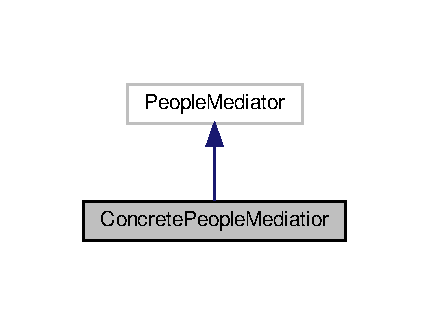
\includegraphics[width=206pt]{classConcretePeopleMediatior__inherit__graph}
\end{center}
\end{figure}


Collaboration diagram for Concrete\+People\+Mediatior\+:\nopagebreak
\begin{figure}[H]
\begin{center}
\leavevmode
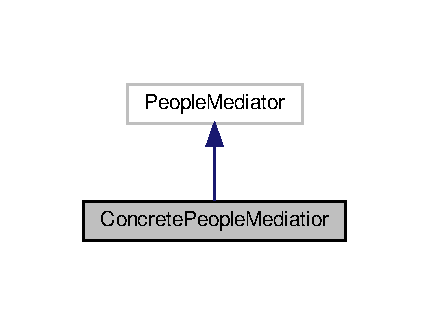
\includegraphics[width=206pt]{classConcretePeopleMediatior__coll__graph}
\end{center}
\end{figure}


The documentation for this class was generated from the following file\+:\begin{DoxyCompactItemize}
\item 
Concrete\+People\+Mediator.\+h\end{DoxyCompactItemize}

\hypertarget{classCritter}{}\section{Critter Class Reference}
\label{classCritter}\index{Critter@{Critter}}


\hyperlink{classCritter}{Critter} class.  




{\ttfamily \#include $<$Critter.\+h$>$}

\subsection*{Public Member Functions}
\begin{DoxyCompactItemize}
\item 
\hyperlink{classCritter_a05aa21e3b570d7380f3ead47c99442ef}{Critter} ()
\item 
bool \hyperlink{classCritter_ab8433b695b842ed8c5593e2f050329de}{is\+Angry} ()
\item 
int \hyperlink{classCritter_a222b3fd7953904ef94dbc0a795c3da56}{steal\+Resources} ()
\end{DoxyCompactItemize}


\subsection{Detailed Description}
\hyperlink{classCritter}{Critter} class. 

\subsection{Constructor \& Destructor Documentation}
\mbox{\Hypertarget{classCritter_a05aa21e3b570d7380f3ead47c99442ef}\label{classCritter_a05aa21e3b570d7380f3ead47c99442ef}} 
\index{Critter@{Critter}!Critter@{Critter}}
\index{Critter@{Critter}!Critter@{Critter}}
\subsubsection{\texorpdfstring{Critter()}{Critter()}}
{\footnotesize\ttfamily Critter\+::\+Critter (\begin{DoxyParamCaption}{ }\end{DoxyParamCaption})}

Default constructor to create critters. Randomly assignes resources and affinity to the critter 

\subsection{Member Function Documentation}
\mbox{\Hypertarget{classCritter_ab8433b695b842ed8c5593e2f050329de}\label{classCritter_ab8433b695b842ed8c5593e2f050329de}} 
\index{Critter@{Critter}!is\+Angry@{is\+Angry}}
\index{is\+Angry@{is\+Angry}!Critter@{Critter}}
\subsubsection{\texorpdfstring{is\+Angry()}{isAngry()}}
{\footnotesize\ttfamily bool Critter\+::is\+Angry (\begin{DoxyParamCaption}{ }\end{DoxyParamCaption})}

\hyperlink{classCritter_ab8433b695b842ed8c5593e2f050329de}{is\+Angry()} returns true if the critter is hostile \begin{DoxyReturn}{Returns}
bool 
\end{DoxyReturn}
\mbox{\Hypertarget{classCritter_a222b3fd7953904ef94dbc0a795c3da56}\label{classCritter_a222b3fd7953904ef94dbc0a795c3da56}} 
\index{Critter@{Critter}!steal\+Resources@{steal\+Resources}}
\index{steal\+Resources@{steal\+Resources}!Critter@{Critter}}
\subsubsection{\texorpdfstring{steal\+Resources()}{stealResources()}}
{\footnotesize\ttfamily int Critter\+::steal\+Resources (\begin{DoxyParamCaption}{ }\end{DoxyParamCaption})}

\hyperlink{classCritter_a222b3fd7953904ef94dbc0a795c3da56}{steal\+Resources()} If the critter is captured you will be able to take all the resources that the critter holds \begin{DoxyReturn}{Returns}
int -\/ \textquotesingle{}-\/1\textquotesingle{} on making the critter angry 
\end{DoxyReturn}


The documentation for this class was generated from the following files\+:\begin{DoxyCompactItemize}
\item 
Critter.\+h\item 
Critter.\+cpp\end{DoxyCompactItemize}

\hypertarget{classDoctor}{}\section{Doctor Class Reference}
\label{classDoctor}\index{Doctor@{Doctor}}


\hyperlink{classDoctor}{Doctor} class.  




{\ttfamily \#include $<$Doctor.\+h$>$}



Inheritance diagram for Doctor\+:
% FIG 0


Collaboration diagram for Doctor\+:
% FIG 1
\subsection*{Public Member Functions}
\begin{DoxyCompactItemize}
\item 
\hyperlink{classDoctor_ac71a90316796a8e72a8d9db536de274a}{Doctor} ()
\item 
\hyperlink{classDoctor_a1481ccfafebc7a2424d3659a0223ebfe}{$\sim$\+Doctor} ()
\item 
void \hyperlink{classDoctor_a820dca3b9f05d3f69c47bd7318923b88}{recieve\+Spaceship\+Error} (string)
\item 
void \hyperlink{classDoctor_a5a524981ce52102f975cf9c569137ce5}{send\+Error\+Message} (string)
\end{DoxyCompactItemize}
\subsection*{Additional Inherited Members}


\subsection{Detailed Description}
\hyperlink{classDoctor}{Doctor} class. 

\subsection{Constructor \& Destructor Documentation}
\mbox{\Hypertarget{classDoctor_ac71a90316796a8e72a8d9db536de274a}\label{classDoctor_ac71a90316796a8e72a8d9db536de274a}} 
\index{Doctor@{Doctor}!Doctor@{Doctor}}
\index{Doctor@{Doctor}!Doctor@{Doctor}}
\subsubsection{\texorpdfstring{Doctor()}{Doctor()}}
{\footnotesize\ttfamily Doctor\+::\+Doctor (\begin{DoxyParamCaption}{ }\end{DoxyParamCaption})\hspace{0.3cm}{\ttfamily [inline]}}

Default constructor \mbox{\Hypertarget{classDoctor_a1481ccfafebc7a2424d3659a0223ebfe}\label{classDoctor_a1481ccfafebc7a2424d3659a0223ebfe}} 
\index{Doctor@{Doctor}!````~Doctor@{$\sim$\+Doctor}}
\index{````~Doctor@{$\sim$\+Doctor}!Doctor@{Doctor}}
\subsubsection{\texorpdfstring{$\sim$\+Doctor()}{~Doctor()}}
{\footnotesize\ttfamily Doctor\+::$\sim$\+Doctor (\begin{DoxyParamCaption}{ }\end{DoxyParamCaption})\hspace{0.3cm}{\ttfamily [inline]}}

Default destructor 

\subsection{Member Function Documentation}
\mbox{\Hypertarget{classDoctor_a820dca3b9f05d3f69c47bd7318923b88}\label{classDoctor_a820dca3b9f05d3f69c47bd7318923b88}} 
\index{Doctor@{Doctor}!recieve\+Spaceship\+Error@{recieve\+Spaceship\+Error}}
\index{recieve\+Spaceship\+Error@{recieve\+Spaceship\+Error}!Doctor@{Doctor}}
\subsubsection{\texorpdfstring{recieve\+Spaceship\+Error()}{recieveSpaceshipError()}}
{\footnotesize\ttfamily void Doctor\+::recieve\+Spaceship\+Error (\begin{DoxyParamCaption}\item[{string}]{message }\end{DoxyParamCaption})\hspace{0.3cm}{\ttfamily [virtual]}}

Receive an error from the spaceship 
\begin{DoxyParams}{Parameters}
{\em message} & -\/ the message being received \\
\hline
\end{DoxyParams}


Implements \hyperlink{classPeople_a0685df78be631783138865e03cc7c85d}{People}.

\mbox{\Hypertarget{classDoctor_a5a524981ce52102f975cf9c569137ce5}\label{classDoctor_a5a524981ce52102f975cf9c569137ce5}} 
\index{Doctor@{Doctor}!send\+Error\+Message@{send\+Error\+Message}}
\index{send\+Error\+Message@{send\+Error\+Message}!Doctor@{Doctor}}
\subsubsection{\texorpdfstring{send\+Error\+Message()}{sendErrorMessage()}}
{\footnotesize\ttfamily void Doctor\+::send\+Error\+Message (\begin{DoxyParamCaption}\item[{string}]{message }\end{DoxyParamCaption})\hspace{0.3cm}{\ttfamily [virtual]}}

Send an error to the spaceship 
\begin{DoxyParams}{Parameters}
{\em message} & -\/ the message being sent \\
\hline
\end{DoxyParams}


Implements \hyperlink{classPeople_a572a35170f61d1848eb04b65baafb057}{People}.



The documentation for this class was generated from the following files\+:\begin{DoxyCompactItemize}
\item 
Doctor.\+h\item 
Doctor.\+cpp\end{DoxyCompactItemize}

\hypertarget{classDoctorFactory}{}\section{Doctor\+Factory Class Reference}
\label{classDoctorFactory}\index{Doctor\+Factory@{Doctor\+Factory}}


\hyperlink{classDoctor}{Doctor} Factory class.  




{\ttfamily \#include $<$Doctor\+Factory.\+h$>$}



Inheritance diagram for Doctor\+Factory\+:
% FIG 0


Collaboration diagram for Doctor\+Factory\+:
% FIG 1
\subsection*{Public Member Functions}
\begin{DoxyCompactItemize}
\item 
\hyperlink{classDoctorFactory_aadc371102a234a3a86f46e029f6cf6fe}{Doctor\+Factory} ()
\item 
\hyperlink{classDoctorFactory_a3f2ed2a1a4378d3490c0412645f70767}{$\sim$\+Doctor\+Factory} ()
\item 
virtual \hyperlink{classPeople}{People} $\ast$ \hyperlink{classDoctorFactory_a2fead4ec5680093ba93fde6b1b734c59}{create\+People} ()=0
\end{DoxyCompactItemize}
\subsection*{Additional Inherited Members}


\subsection{Detailed Description}
\hyperlink{classDoctor}{Doctor} Factory class. 

\subsection{Constructor \& Destructor Documentation}
\mbox{\Hypertarget{classDoctorFactory_aadc371102a234a3a86f46e029f6cf6fe}\label{classDoctorFactory_aadc371102a234a3a86f46e029f6cf6fe}} 
\index{Doctor\+Factory@{Doctor\+Factory}!Doctor\+Factory@{Doctor\+Factory}}
\index{Doctor\+Factory@{Doctor\+Factory}!Doctor\+Factory@{Doctor\+Factory}}
\subsubsection{\texorpdfstring{Doctor\+Factory()}{DoctorFactory()}}
{\footnotesize\ttfamily Doctor\+Factory\+::\+Doctor\+Factory (\begin{DoxyParamCaption}{ }\end{DoxyParamCaption})}

Default constructor \mbox{\Hypertarget{classDoctorFactory_a3f2ed2a1a4378d3490c0412645f70767}\label{classDoctorFactory_a3f2ed2a1a4378d3490c0412645f70767}} 
\index{Doctor\+Factory@{Doctor\+Factory}!````~Doctor\+Factory@{$\sim$\+Doctor\+Factory}}
\index{````~Doctor\+Factory@{$\sim$\+Doctor\+Factory}!Doctor\+Factory@{Doctor\+Factory}}
\subsubsection{\texorpdfstring{$\sim$\+Doctor\+Factory()}{~DoctorFactory()}}
{\footnotesize\ttfamily Doctor\+Factory\+::$\sim$\+Doctor\+Factory (\begin{DoxyParamCaption}{ }\end{DoxyParamCaption})}

Default destructor 

\subsection{Member Function Documentation}
\mbox{\Hypertarget{classDoctorFactory_a2fead4ec5680093ba93fde6b1b734c59}\label{classDoctorFactory_a2fead4ec5680093ba93fde6b1b734c59}} 
\index{Doctor\+Factory@{Doctor\+Factory}!create\+People@{create\+People}}
\index{create\+People@{create\+People}!Doctor\+Factory@{Doctor\+Factory}}
\subsubsection{\texorpdfstring{create\+People()}{createPeople()}}
{\footnotesize\ttfamily virtual \hyperlink{classPeople}{People}$\ast$ Doctor\+Factory\+::create\+People (\begin{DoxyParamCaption}{ }\end{DoxyParamCaption})\hspace{0.3cm}{\ttfamily [pure virtual]}}

virtual doctor 

The documentation for this class was generated from the following file\+:\begin{DoxyCompactItemize}
\item 
Doctor\+Factory.\+h\end{DoxyCompactItemize}

\hypertarget{classEngineer}{}\section{Engineer Class Reference}
\label{classEngineer}\index{Engineer@{Engineer}}


\hyperlink{classEngineer}{Engineer} class.  




{\ttfamily \#include $<$Engineer.\+h$>$}



Inheritance diagram for Engineer\+:\nopagebreak
\begin{figure}[H]
\begin{center}
\leavevmode
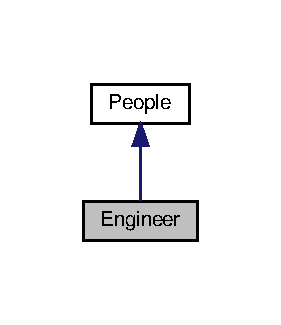
\includegraphics[width=135pt]{classEngineer__inherit__graph}
\end{center}
\end{figure}


Collaboration diagram for Engineer\+:\nopagebreak
\begin{figure}[H]
\begin{center}
\leavevmode
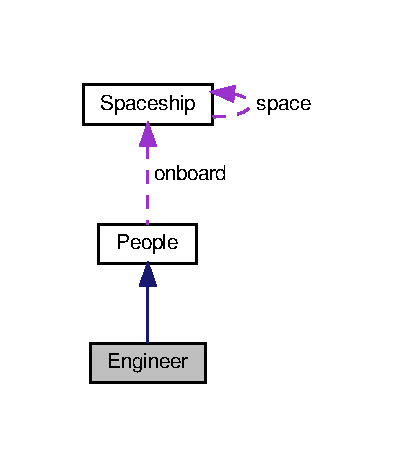
\includegraphics[width=190pt]{classEngineer__coll__graph}
\end{center}
\end{figure}
\subsection*{Public Member Functions}
\begin{DoxyCompactItemize}
\item 
\hyperlink{classEngineer_acf0604e3e44a09583b420c729b651ad7}{Engineer} ()
\item 
\hyperlink{classPeople}{People} $\ast$ \hyperlink{classEngineer_aaa9d760e22cab80ec283b2a085782feb}{create\+People} ()
\item 
void \hyperlink{classEngineer_acc86ce6b4b1388be8ebacc685f9e6233}{recieve\+Spaceship\+Error} (string)
\item 
void \hyperlink{classEngineer_ae60806f33b7f226891dbb7ad9b8a0c0b}{send\+Error\+Message} (string)
\item 
string \hyperlink{classEngineer_ae2f83b9c2df3e8d3937697b23546571a}{get\+Type} ()
\end{DoxyCompactItemize}
\subsection*{Additional Inherited Members}


\subsection{Detailed Description}
\hyperlink{classEngineer}{Engineer} class. 

\subsection{Constructor \& Destructor Documentation}
\mbox{\Hypertarget{classEngineer_acf0604e3e44a09583b420c729b651ad7}\label{classEngineer_acf0604e3e44a09583b420c729b651ad7}} 
\index{Engineer@{Engineer}!Engineer@{Engineer}}
\index{Engineer@{Engineer}!Engineer@{Engineer}}
\subsubsection{\texorpdfstring{Engineer()}{Engineer()}}
{\footnotesize\ttfamily Engineer\+::\+Engineer (\begin{DoxyParamCaption}{ }\end{DoxyParamCaption})\hspace{0.3cm}{\ttfamily [inline]}}

Default constructor 

\subsection{Member Function Documentation}
\mbox{\Hypertarget{classEngineer_aaa9d760e22cab80ec283b2a085782feb}\label{classEngineer_aaa9d760e22cab80ec283b2a085782feb}} 
\index{Engineer@{Engineer}!create\+People@{create\+People}}
\index{create\+People@{create\+People}!Engineer@{Engineer}}
\subsubsection{\texorpdfstring{create\+People()}{createPeople()}}
{\footnotesize\ttfamily \hyperlink{classPeople}{People}$\ast$ Engineer\+::create\+People (\begin{DoxyParamCaption}{ }\end{DoxyParamCaption})}

Default desctructor creates \hyperlink{classEngineer}{Engineer} \mbox{\Hypertarget{classEngineer_ae2f83b9c2df3e8d3937697b23546571a}\label{classEngineer_ae2f83b9c2df3e8d3937697b23546571a}} 
\index{Engineer@{Engineer}!get\+Type@{get\+Type}}
\index{get\+Type@{get\+Type}!Engineer@{Engineer}}
\subsubsection{\texorpdfstring{get\+Type()}{getType()}}
{\footnotesize\ttfamily string Engineer\+::get\+Type (\begin{DoxyParamCaption}{ }\end{DoxyParamCaption})\hspace{0.3cm}{\ttfamily [inline]}, {\ttfamily [virtual]}}

get type of the person 

Implements \hyperlink{classPeople_af60dd882d60cddf63f9b95815ce551a8}{People}.

\mbox{\Hypertarget{classEngineer_acc86ce6b4b1388be8ebacc685f9e6233}\label{classEngineer_acc86ce6b4b1388be8ebacc685f9e6233}} 
\index{Engineer@{Engineer}!recieve\+Spaceship\+Error@{recieve\+Spaceship\+Error}}
\index{recieve\+Spaceship\+Error@{recieve\+Spaceship\+Error}!Engineer@{Engineer}}
\subsubsection{\texorpdfstring{recieve\+Spaceship\+Error()}{recieveSpaceshipError()}}
{\footnotesize\ttfamily void Engineer\+::recieve\+Spaceship\+Error (\begin{DoxyParamCaption}\item[{string}]{message }\end{DoxyParamCaption})\hspace{0.3cm}{\ttfamily [virtual]}}

Recieve an error from the spaceship 
\begin{DoxyParams}{Parameters}
{\em message} & -\/ the message being recieved \\
\hline
\end{DoxyParams}


Implements \hyperlink{classPeople_a0685df78be631783138865e03cc7c85d}{People}.

\mbox{\Hypertarget{classEngineer_ae60806f33b7f226891dbb7ad9b8a0c0b}\label{classEngineer_ae60806f33b7f226891dbb7ad9b8a0c0b}} 
\index{Engineer@{Engineer}!send\+Error\+Message@{send\+Error\+Message}}
\index{send\+Error\+Message@{send\+Error\+Message}!Engineer@{Engineer}}
\subsubsection{\texorpdfstring{send\+Error\+Message()}{sendErrorMessage()}}
{\footnotesize\ttfamily void Engineer\+::send\+Error\+Message (\begin{DoxyParamCaption}\item[{string}]{message }\end{DoxyParamCaption})\hspace{0.3cm}{\ttfamily [virtual]}}

Send an error to the spaceship 
\begin{DoxyParams}{Parameters}
{\em message} & -\/ the message being sent \\
\hline
\end{DoxyParams}


Implements \hyperlink{classPeople_a572a35170f61d1848eb04b65baafb057}{People}.



The documentation for this class was generated from the following files\+:\begin{DoxyCompactItemize}
\item 
Engineer.\+h\item 
Engineer.\+cpp\end{DoxyCompactItemize}

\hypertarget{classEngineerFactory}{}\section{Engineer\+Factory Class Reference}
\label{classEngineerFactory}\index{Engineer\+Factory@{Engineer\+Factory}}


\hyperlink{classEngineer}{Engineer} Factory class.  




{\ttfamily \#include $<$Engineer\+Factory.\+h$>$}



Inheritance diagram for Engineer\+Factory\+:\nopagebreak
\begin{figure}[H]
\begin{center}
\leavevmode
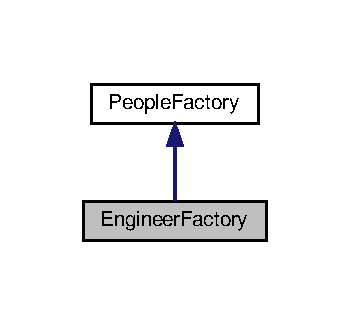
\includegraphics[width=168pt]{classEngineerFactory__inherit__graph}
\end{center}
\end{figure}


Collaboration diagram for Engineer\+Factory\+:\nopagebreak
\begin{figure}[H]
\begin{center}
\leavevmode
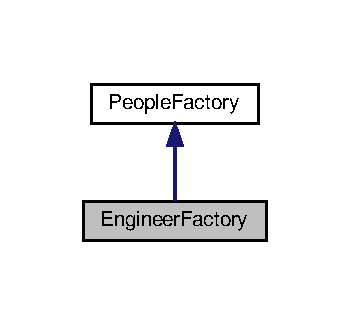
\includegraphics[width=168pt]{classEngineerFactory__coll__graph}
\end{center}
\end{figure}
\subsection*{Public Member Functions}
\begin{DoxyCompactItemize}
\item 
\hyperlink{classEngineerFactory_a71b5abb3e85ebe5f78eaafc388d0ed2d}{Engineer\+Factory} ()
\item 
\hyperlink{classEngineerFactory_af892e0d4b047414dbcefee0bbe943208}{$\sim$\+Engineer\+Factory} ()
\item 
\hyperlink{classPeople}{People} $\ast$ \hyperlink{classEngineerFactory_a7a66d4957f1f9b821771c43e5af289f2}{create} ()
\end{DoxyCompactItemize}


\subsection{Detailed Description}
\hyperlink{classEngineer}{Engineer} Factory class. 

\subsection{Constructor \& Destructor Documentation}
\mbox{\Hypertarget{classEngineerFactory_a71b5abb3e85ebe5f78eaafc388d0ed2d}\label{classEngineerFactory_a71b5abb3e85ebe5f78eaafc388d0ed2d}} 
\index{Engineer\+Factory@{Engineer\+Factory}!Engineer\+Factory@{Engineer\+Factory}}
\index{Engineer\+Factory@{Engineer\+Factory}!Engineer\+Factory@{Engineer\+Factory}}
\subsubsection{\texorpdfstring{Engineer\+Factory()}{EngineerFactory()}}
{\footnotesize\ttfamily Engineer\+Factory\+::\+Engineer\+Factory (\begin{DoxyParamCaption}{ }\end{DoxyParamCaption})\hspace{0.3cm}{\ttfamily [inline]}}

Default constructor \mbox{\Hypertarget{classEngineerFactory_af892e0d4b047414dbcefee0bbe943208}\label{classEngineerFactory_af892e0d4b047414dbcefee0bbe943208}} 
\index{Engineer\+Factory@{Engineer\+Factory}!````~Engineer\+Factory@{$\sim$\+Engineer\+Factory}}
\index{````~Engineer\+Factory@{$\sim$\+Engineer\+Factory}!Engineer\+Factory@{Engineer\+Factory}}
\subsubsection{\texorpdfstring{$\sim$\+Engineer\+Factory()}{~EngineerFactory()}}
{\footnotesize\ttfamily Engineer\+Factory\+::$\sim$\+Engineer\+Factory (\begin{DoxyParamCaption}{ }\end{DoxyParamCaption})\hspace{0.3cm}{\ttfamily [inline]}}

Default desctructor 

\subsection{Member Function Documentation}
\mbox{\Hypertarget{classEngineerFactory_a7a66d4957f1f9b821771c43e5af289f2}\label{classEngineerFactory_a7a66d4957f1f9b821771c43e5af289f2}} 
\index{Engineer\+Factory@{Engineer\+Factory}!create@{create}}
\index{create@{create}!Engineer\+Factory@{Engineer\+Factory}}
\subsubsection{\texorpdfstring{create()}{create()}}
{\footnotesize\ttfamily \hyperlink{classPeople}{People}$\ast$ Engineer\+Factory\+::create (\begin{DoxyParamCaption}{ }\end{DoxyParamCaption})\hspace{0.3cm}{\ttfamily [inline]}, {\ttfamily [virtual]}}

virtual \hyperlink{classEngineer}{Engineer} 

Implements \hyperlink{classPeopleFactory}{People\+Factory}.



The documentation for this class was generated from the following file\+:\begin{DoxyCompactItemize}
\item 
Engineer\+Factory.\+h\end{DoxyCompactItemize}

\hypertarget{classExplorationVessel}{}\section{Exploration\+Vessel Class Reference}
\label{classExplorationVessel}\index{Exploration\+Vessel@{Exploration\+Vessel}}


Exploration Vessel class.  




{\ttfamily \#include $<$Exploration\+Vessel.\+h$>$}



Inheritance diagram for Exploration\+Vessel\+:\nopagebreak
\begin{figure}[H]
\begin{center}
\leavevmode
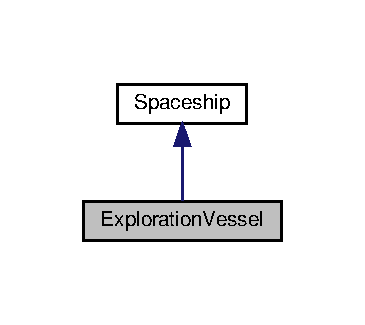
\includegraphics[width=175pt]{classExplorationVessel__inherit__graph}
\end{center}
\end{figure}


Collaboration diagram for Exploration\+Vessel\+:\nopagebreak
\begin{figure}[H]
\begin{center}
\leavevmode
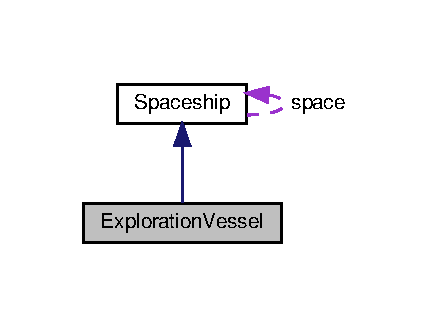
\includegraphics[width=207pt]{classExplorationVessel__coll__graph}
\end{center}
\end{figure}
\subsection*{Public Member Functions}
\begin{DoxyCompactItemize}
\item 
\hyperlink{classExplorationVessel_ab664e2a5b901063c15d86e13f3b981f6}{Exploration\+Vessel} ()
\item 
\hyperlink{classExplorationVessel_ac7b29c63250f7263808af4e21e412cce}{$\sim$\+Exploration\+Vessel} ()
\item 
\hyperlink{classExplorationVessel_acc004a39ae71f367d3bca876fb02e9c5}{Exploration\+Vessel} (string name)
\item 
virtual void \hyperlink{classExplorationVessel_ae952e198a28fd0a5ec998ecdcca86561}{add\+Component} (\hyperlink{classSpaceship}{Spaceship} $\ast$comp)
\item 
void \hyperlink{classExplorationVessel_a31ce2f706dab569719ec91db00ecc49d}{visit} (\hyperlink{classPlanet}{Planet} $\ast$p)
\item 
int \hyperlink{classExplorationVessel_ab06e219200100bbd40a8f79702e52ae8}{get\+Type} ()
\item 
void \hyperlink{classExplorationVessel_a2f164fa9477a2624c5f04b4d9d84ec84}{increase\+Threat\+Level} ()
\item 
void \hyperlink{classExplorationVessel_afac2ec0016d6934629418074e3de5950}{decrease\+Threat\+Level} ()
\item 
void \hyperlink{classExplorationVessel_af08a3db5b456781106f33a03bfbe7621}{print\+Threat\+Level} ()
\item 
void \hyperlink{classExplorationVessel_a83a2bacf57d718eb75ba033bbe363b9e}{execute\+Strategy} ()
\item 
void \hyperlink{classExplorationVessel_aeaec72883c8cc5b951be9dd8f4184515}{select\+Strategy} (\hyperlink{classStrategy}{Strategy} $\ast$s)
\item 
void \hyperlink{classExplorationVessel_ac6bc6807891edf928fae68e7ed850d14}{add\+Ship} (\hyperlink{classSpaceship}{Spaceship} $\ast$s)
\item 
double \hyperlink{classExplorationVessel_a3c3a641c6c249f80d68f20cf73f440f7}{get\+Resources} (double a, double b)
\item 
void \hyperlink{classExplorationVessel_a7be654e42a9e83800abfb897d9b308b8}{add\+Person} (\hyperlink{classPeople}{People} $\ast$p)
\item 
\hyperlink{classMemento}{Memento} $\ast$ \hyperlink{classExplorationVessel_a90a2c653d736fadf0599af87269fa36e}{create\+Memento} (vector$<$ \hyperlink{classSpaceship}{Spaceship} $\ast$$>$ s)
\item 
void \hyperlink{classExplorationVessel_a314e19ec45f722d80adb800eb7b36d20}{reinstate\+Memento} (\hyperlink{classMemento}{Memento} $\ast$mem)
\end{DoxyCompactItemize}
\subsection*{Additional Inherited Members}


\subsection{Detailed Description}
Exploration Vessel class. 

\subsection{Constructor \& Destructor Documentation}
\mbox{\Hypertarget{classExplorationVessel_ab664e2a5b901063c15d86e13f3b981f6}\label{classExplorationVessel_ab664e2a5b901063c15d86e13f3b981f6}} 
\index{Exploration\+Vessel@{Exploration\+Vessel}!Exploration\+Vessel@{Exploration\+Vessel}}
\index{Exploration\+Vessel@{Exploration\+Vessel}!Exploration\+Vessel@{Exploration\+Vessel}}
\subsubsection{\texorpdfstring{Exploration\+Vessel()}{ExplorationVessel()}\hspace{0.1cm}{\footnotesize\ttfamily [1/2]}}
{\footnotesize\ttfamily Exploration\+Vessel\+::\+Exploration\+Vessel (\begin{DoxyParamCaption}{ }\end{DoxyParamCaption})\hspace{0.3cm}{\ttfamily [inline]}}

Default constructor \mbox{\Hypertarget{classExplorationVessel_ac7b29c63250f7263808af4e21e412cce}\label{classExplorationVessel_ac7b29c63250f7263808af4e21e412cce}} 
\index{Exploration\+Vessel@{Exploration\+Vessel}!````~Exploration\+Vessel@{$\sim$\+Exploration\+Vessel}}
\index{````~Exploration\+Vessel@{$\sim$\+Exploration\+Vessel}!Exploration\+Vessel@{Exploration\+Vessel}}
\subsubsection{\texorpdfstring{$\sim$\+Exploration\+Vessel()}{~ExplorationVessel()}}
{\footnotesize\ttfamily Exploration\+Vessel\+::$\sim$\+Exploration\+Vessel (\begin{DoxyParamCaption}{ }\end{DoxyParamCaption})\hspace{0.3cm}{\ttfamily [inline]}}

Default desctructor \mbox{\Hypertarget{classExplorationVessel_acc004a39ae71f367d3bca876fb02e9c5}\label{classExplorationVessel_acc004a39ae71f367d3bca876fb02e9c5}} 
\index{Exploration\+Vessel@{Exploration\+Vessel}!Exploration\+Vessel@{Exploration\+Vessel}}
\index{Exploration\+Vessel@{Exploration\+Vessel}!Exploration\+Vessel@{Exploration\+Vessel}}
\subsubsection{\texorpdfstring{Exploration\+Vessel()}{ExplorationVessel()}\hspace{0.1cm}{\footnotesize\ttfamily [2/2]}}
{\footnotesize\ttfamily Exploration\+Vessel\+::\+Exploration\+Vessel (\begin{DoxyParamCaption}\item[{string}]{name }\end{DoxyParamCaption})\hspace{0.3cm}{\ttfamily [inline]}}

Paramaterised constructor 

\subsection{Member Function Documentation}
\mbox{\Hypertarget{classExplorationVessel_ae952e198a28fd0a5ec998ecdcca86561}\label{classExplorationVessel_ae952e198a28fd0a5ec998ecdcca86561}} 
\index{Exploration\+Vessel@{Exploration\+Vessel}!add\+Component@{add\+Component}}
\index{add\+Component@{add\+Component}!Exploration\+Vessel@{Exploration\+Vessel}}
\subsubsection{\texorpdfstring{add\+Component()}{addComponent()}}
{\footnotesize\ttfamily virtual void Exploration\+Vessel\+::add\+Component (\begin{DoxyParamCaption}\item[{\hyperlink{classSpaceship}{Spaceship} $\ast$}]{comp }\end{DoxyParamCaption})\hspace{0.3cm}{\ttfamily [inline]}, {\ttfamily [virtual]}}

Add a component to the vessel 
\begin{DoxyParams}{Parameters}
{\em s} & -\/ spaceship component to be added \\
\hline
\end{DoxyParams}


Implements \hyperlink{classSpaceship_ac1b4673a691cd100708ddea08cd9f192}{Spaceship}.

\mbox{\Hypertarget{classExplorationVessel_a7be654e42a9e83800abfb897d9b308b8}\label{classExplorationVessel_a7be654e42a9e83800abfb897d9b308b8}} 
\index{Exploration\+Vessel@{Exploration\+Vessel}!add\+Person@{add\+Person}}
\index{add\+Person@{add\+Person}!Exploration\+Vessel@{Exploration\+Vessel}}
\subsubsection{\texorpdfstring{add\+Person()}{addPerson()}}
{\footnotesize\ttfamily void Exploration\+Vessel\+::add\+Person (\begin{DoxyParamCaption}\item[{\hyperlink{classPeople}{People} $\ast$}]{p }\end{DoxyParamCaption})\hspace{0.3cm}{\ttfamily [inline]}, {\ttfamily [virtual]}}

stub for add\+Person 

Reimplemented from \hyperlink{classSpaceship_add8d9c6dfd5f6ecb8399e41e71e5b22f}{Spaceship}.

\mbox{\Hypertarget{classExplorationVessel_ac6bc6807891edf928fae68e7ed850d14}\label{classExplorationVessel_ac6bc6807891edf928fae68e7ed850d14}} 
\index{Exploration\+Vessel@{Exploration\+Vessel}!add\+Ship@{add\+Ship}}
\index{add\+Ship@{add\+Ship}!Exploration\+Vessel@{Exploration\+Vessel}}
\subsubsection{\texorpdfstring{add\+Ship()}{addShip()}}
{\footnotesize\ttfamily void Exploration\+Vessel\+::add\+Ship (\begin{DoxyParamCaption}\item[{\hyperlink{classSpaceship}{Spaceship} $\ast$}]{ }\end{DoxyParamCaption})\hspace{0.3cm}{\ttfamily [inline]}, {\ttfamily [virtual]}}

Virtual add\+Ship 

Reimplemented from \hyperlink{classSpaceship_a90e1321cdbcb459b98b75ab39cef867d}{Spaceship}.

\mbox{\Hypertarget{classExplorationVessel_a90a2c653d736fadf0599af87269fa36e}\label{classExplorationVessel_a90a2c653d736fadf0599af87269fa36e}} 
\index{Exploration\+Vessel@{Exploration\+Vessel}!create\+Memento@{create\+Memento}}
\index{create\+Memento@{create\+Memento}!Exploration\+Vessel@{Exploration\+Vessel}}
\subsubsection{\texorpdfstring{create\+Memento()}{createMemento()}}
{\footnotesize\ttfamily \hyperlink{classMemento}{Memento}$\ast$ Exploration\+Vessel\+::create\+Memento (\begin{DoxyParamCaption}\item[{vector$<$ \hyperlink{classSpaceship}{Spaceship} $\ast$$>$}]{s }\end{DoxyParamCaption})\hspace{0.3cm}{\ttfamily [inline]}, {\ttfamily [virtual]}}

create memento stub 

Reimplemented from \hyperlink{classSpaceship_a6d272f846b019dec8226ddab65648a7b}{Spaceship}.

\mbox{\Hypertarget{classExplorationVessel_afac2ec0016d6934629418074e3de5950}\label{classExplorationVessel_afac2ec0016d6934629418074e3de5950}} 
\index{Exploration\+Vessel@{Exploration\+Vessel}!decrease\+Threat\+Level@{decrease\+Threat\+Level}}
\index{decrease\+Threat\+Level@{decrease\+Threat\+Level}!Exploration\+Vessel@{Exploration\+Vessel}}
\subsubsection{\texorpdfstring{decrease\+Threat\+Level()}{decreaseThreatLevel()}}
{\footnotesize\ttfamily void Exploration\+Vessel\+::decrease\+Threat\+Level (\begin{DoxyParamCaption}{ }\end{DoxyParamCaption})\hspace{0.3cm}{\ttfamily [inline]}, {\ttfamily [virtual]}}

stub for decrease\+Threat\+Level 

Reimplemented from \hyperlink{classSpaceship_a73a1eefd211e9a2063d924ee85f0c0c7}{Spaceship}.

\mbox{\Hypertarget{classExplorationVessel_a83a2bacf57d718eb75ba033bbe363b9e}\label{classExplorationVessel_a83a2bacf57d718eb75ba033bbe363b9e}} 
\index{Exploration\+Vessel@{Exploration\+Vessel}!execute\+Strategy@{execute\+Strategy}}
\index{execute\+Strategy@{execute\+Strategy}!Exploration\+Vessel@{Exploration\+Vessel}}
\subsubsection{\texorpdfstring{execute\+Strategy()}{executeStrategy()}}
{\footnotesize\ttfamily void Exploration\+Vessel\+::execute\+Strategy (\begin{DoxyParamCaption}{ }\end{DoxyParamCaption})\hspace{0.3cm}{\ttfamily [inline]}, {\ttfamily [virtual]}}

execute strategy 

Reimplemented from \hyperlink{classSpaceship}{Spaceship}.

\mbox{\Hypertarget{classExplorationVessel_a3c3a641c6c249f80d68f20cf73f440f7}\label{classExplorationVessel_a3c3a641c6c249f80d68f20cf73f440f7}} 
\index{Exploration\+Vessel@{Exploration\+Vessel}!get\+Resources@{get\+Resources}}
\index{get\+Resources@{get\+Resources}!Exploration\+Vessel@{Exploration\+Vessel}}
\subsubsection{\texorpdfstring{get\+Resources()}{getResources()}}
{\footnotesize\ttfamily double Exploration\+Vessel\+::get\+Resources (\begin{DoxyParamCaption}\item[{double}]{a,  }\item[{double}]{b }\end{DoxyParamCaption})\hspace{0.3cm}{\ttfamily [inline]}, {\ttfamily [virtual]}}

stub resource collection 

Reimplemented from \hyperlink{classSpaceship_ad2027533de1d789db5e3efa22055f2d0}{Spaceship}.

\mbox{\Hypertarget{classExplorationVessel_ab06e219200100bbd40a8f79702e52ae8}\label{classExplorationVessel_ab06e219200100bbd40a8f79702e52ae8}} 
\index{Exploration\+Vessel@{Exploration\+Vessel}!get\+Type@{get\+Type}}
\index{get\+Type@{get\+Type}!Exploration\+Vessel@{Exploration\+Vessel}}
\subsubsection{\texorpdfstring{get\+Type()}{getType()}}
{\footnotesize\ttfamily int Exploration\+Vessel\+::get\+Type (\begin{DoxyParamCaption}{ }\end{DoxyParamCaption})\hspace{0.3cm}{\ttfamily [inline]}, {\ttfamily [virtual]}}

Get type of spaceship -\/ \hyperlink{classExplorationVessel}{Exploration\+Vessel} = 2 \begin{DoxyReturn}{Returns}
int -\/ 2 
\end{DoxyReturn}


Reimplemented from \hyperlink{classSpaceship_a113055e6d793f8fbc55e44efc4d57e07}{Spaceship}.

\mbox{\Hypertarget{classExplorationVessel_a2f164fa9477a2624c5f04b4d9d84ec84}\label{classExplorationVessel_a2f164fa9477a2624c5f04b4d9d84ec84}} 
\index{Exploration\+Vessel@{Exploration\+Vessel}!increase\+Threat\+Level@{increase\+Threat\+Level}}
\index{increase\+Threat\+Level@{increase\+Threat\+Level}!Exploration\+Vessel@{Exploration\+Vessel}}
\subsubsection{\texorpdfstring{increase\+Threat\+Level()}{increaseThreatLevel()}}
{\footnotesize\ttfamily void Exploration\+Vessel\+::increase\+Threat\+Level (\begin{DoxyParamCaption}{ }\end{DoxyParamCaption})\hspace{0.3cm}{\ttfamily [inline]}, {\ttfamily [virtual]}}

stub for increase\+Threat\+Level 

Reimplemented from \hyperlink{classSpaceship_a5ddf702124286d9d3a6b5e64c09515bc}{Spaceship}.

\mbox{\Hypertarget{classExplorationVessel_af08a3db5b456781106f33a03bfbe7621}\label{classExplorationVessel_af08a3db5b456781106f33a03bfbe7621}} 
\index{Exploration\+Vessel@{Exploration\+Vessel}!print\+Threat\+Level@{print\+Threat\+Level}}
\index{print\+Threat\+Level@{print\+Threat\+Level}!Exploration\+Vessel@{Exploration\+Vessel}}
\subsubsection{\texorpdfstring{print\+Threat\+Level()}{printThreatLevel()}}
{\footnotesize\ttfamily void Exploration\+Vessel\+::print\+Threat\+Level (\begin{DoxyParamCaption}{ }\end{DoxyParamCaption})\hspace{0.3cm}{\ttfamily [inline]}, {\ttfamily [virtual]}}

stub for print\+Threat\+Level 

Reimplemented from \hyperlink{classSpaceship_a8f16814f888a5a1423e5a491329cdb97}{Spaceship}.

\mbox{\Hypertarget{classExplorationVessel_a314e19ec45f722d80adb800eb7b36d20}\label{classExplorationVessel_a314e19ec45f722d80adb800eb7b36d20}} 
\index{Exploration\+Vessel@{Exploration\+Vessel}!reinstate\+Memento@{reinstate\+Memento}}
\index{reinstate\+Memento@{reinstate\+Memento}!Exploration\+Vessel@{Exploration\+Vessel}}
\subsubsection{\texorpdfstring{reinstate\+Memento()}{reinstateMemento()}}
{\footnotesize\ttfamily void Exploration\+Vessel\+::reinstate\+Memento (\begin{DoxyParamCaption}\item[{\hyperlink{classMemento}{Memento} $\ast$}]{mem }\end{DoxyParamCaption})\hspace{0.3cm}{\ttfamily [inline]}, {\ttfamily [virtual]}}

reinstate memento 

Reimplemented from \hyperlink{classSpaceship_ab075c869473344b6471c8e28ca7ea61e}{Spaceship}.

\mbox{\Hypertarget{classExplorationVessel_aeaec72883c8cc5b951be9dd8f4184515}\label{classExplorationVessel_aeaec72883c8cc5b951be9dd8f4184515}} 
\index{Exploration\+Vessel@{Exploration\+Vessel}!select\+Strategy@{select\+Strategy}}
\index{select\+Strategy@{select\+Strategy}!Exploration\+Vessel@{Exploration\+Vessel}}
\subsubsection{\texorpdfstring{select\+Strategy()}{selectStrategy()}}
{\footnotesize\ttfamily void Exploration\+Vessel\+::select\+Strategy (\begin{DoxyParamCaption}\item[{\hyperlink{classStrategy}{Strategy} $\ast$}]{s }\end{DoxyParamCaption})\hspace{0.3cm}{\ttfamily [inline]}, {\ttfamily [virtual]}}

select strategy 

Reimplemented from \hyperlink{classSpaceship_a93be2d9d2b675ef978d866d4cd7a6524}{Spaceship}.

\mbox{\Hypertarget{classExplorationVessel_a31ce2f706dab569719ec91db00ecc49d}\label{classExplorationVessel_a31ce2f706dab569719ec91db00ecc49d}} 
\index{Exploration\+Vessel@{Exploration\+Vessel}!visit@{visit}}
\index{visit@{visit}!Exploration\+Vessel@{Exploration\+Vessel}}
\subsubsection{\texorpdfstring{visit()}{visit()}}
{\footnotesize\ttfamily void Exploration\+Vessel\+::visit (\begin{DoxyParamCaption}\item[{\hyperlink{classPlanet}{Planet} $\ast$}]{p }\end{DoxyParamCaption})\hspace{0.3cm}{\ttfamily [virtual]}}

Add a visitor to the vessel and planet 
\begin{DoxyParams}{Parameters}
{\em p} & -\/ planet to be visited \\
\hline
\end{DoxyParams}


Reimplemented from \hyperlink{classSpaceship}{Spaceship}.



The documentation for this class was generated from the following files\+:\begin{DoxyCompactItemize}
\item 
Exploration\+Vessel.\+h\item 
Exploration\+Vessel.\+cpp\end{DoxyCompactItemize}

\hypertarget{classExplorationVesselFactory}{}\section{Exploration\+Vessel\+Factory Class Reference}
\label{classExplorationVesselFactory}\index{Exploration\+Vessel\+Factory@{Exploration\+Vessel\+Factory}}


Exploration Vessel Factory class.  




{\ttfamily \#include $<$Exploration\+Vessel\+Factory.\+h$>$}



Inheritance diagram for Exploration\+Vessel\+Factory\+:\nopagebreak
\begin{figure}[H]
\begin{center}
\leavevmode
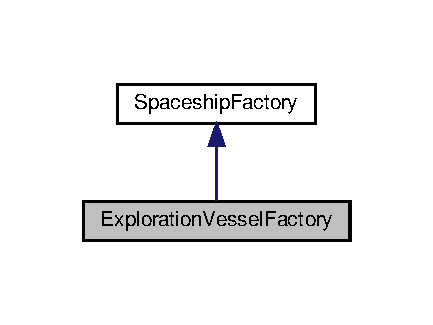
\includegraphics[width=208pt]{classExplorationVesselFactory__inherit__graph}
\end{center}
\end{figure}


Collaboration diagram for Exploration\+Vessel\+Factory\+:\nopagebreak
\begin{figure}[H]
\begin{center}
\leavevmode
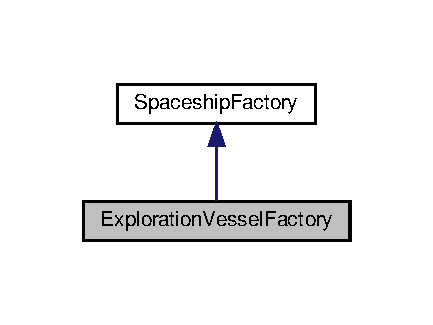
\includegraphics[width=208pt]{classExplorationVesselFactory__coll__graph}
\end{center}
\end{figure}
\subsection*{Public Member Functions}
\begin{DoxyCompactItemize}
\item 
\hyperlink{classExplorationVesselFactory_a4cf974e1ad11c9597a5cd7546a199ded}{Exploration\+Vessel\+Factory} ()
\item 
\hyperlink{classExplorationVesselFactory_a52d1a2adb9d442c82a253de5d68e7b08}{$\sim$\+Exploration\+Vessel\+Factory} ()
\item 
\hyperlink{classSpaceship}{Spaceship} $\ast$ \hyperlink{classExplorationVesselFactory_a67f065b62fedea7805291bd7a3d0b81d}{space\+Ship\+Factory\+Method} (string n)
\end{DoxyCompactItemize}


\subsection{Detailed Description}
Exploration Vessel Factory class. 

\subsection{Constructor \& Destructor Documentation}
\mbox{\Hypertarget{classExplorationVesselFactory_a4cf974e1ad11c9597a5cd7546a199ded}\label{classExplorationVesselFactory_a4cf974e1ad11c9597a5cd7546a199ded}} 
\index{Exploration\+Vessel\+Factory@{Exploration\+Vessel\+Factory}!Exploration\+Vessel\+Factory@{Exploration\+Vessel\+Factory}}
\index{Exploration\+Vessel\+Factory@{Exploration\+Vessel\+Factory}!Exploration\+Vessel\+Factory@{Exploration\+Vessel\+Factory}}
\subsubsection{\texorpdfstring{Exploration\+Vessel\+Factory()}{ExplorationVesselFactory()}}
{\footnotesize\ttfamily Exploration\+Vessel\+Factory\+::\+Exploration\+Vessel\+Factory (\begin{DoxyParamCaption}{ }\end{DoxyParamCaption})}

Defualt constructor \mbox{\Hypertarget{classExplorationVesselFactory_a52d1a2adb9d442c82a253de5d68e7b08}\label{classExplorationVesselFactory_a52d1a2adb9d442c82a253de5d68e7b08}} 
\index{Exploration\+Vessel\+Factory@{Exploration\+Vessel\+Factory}!````~Exploration\+Vessel\+Factory@{$\sim$\+Exploration\+Vessel\+Factory}}
\index{````~Exploration\+Vessel\+Factory@{$\sim$\+Exploration\+Vessel\+Factory}!Exploration\+Vessel\+Factory@{Exploration\+Vessel\+Factory}}
\subsubsection{\texorpdfstring{$\sim$\+Exploration\+Vessel\+Factory()}{~ExplorationVesselFactory()}}
{\footnotesize\ttfamily Exploration\+Vessel\+Factory\+::$\sim$\+Exploration\+Vessel\+Factory (\begin{DoxyParamCaption}{ }\end{DoxyParamCaption})}

Default desctructor 

\subsection{Member Function Documentation}
\mbox{\Hypertarget{classExplorationVesselFactory_a67f065b62fedea7805291bd7a3d0b81d}\label{classExplorationVesselFactory_a67f065b62fedea7805291bd7a3d0b81d}} 
\index{Exploration\+Vessel\+Factory@{Exploration\+Vessel\+Factory}!space\+Ship\+Factory\+Method@{space\+Ship\+Factory\+Method}}
\index{space\+Ship\+Factory\+Method@{space\+Ship\+Factory\+Method}!Exploration\+Vessel\+Factory@{Exploration\+Vessel\+Factory}}
\subsubsection{\texorpdfstring{space\+Ship\+Factory\+Method()}{spaceShipFactoryMethod()}}
{\footnotesize\ttfamily \hyperlink{classSpaceship}{Spaceship} $\ast$ Exploration\+Vessel\+Factory\+::space\+Ship\+Factory\+Method (\begin{DoxyParamCaption}\item[{string}]{n }\end{DoxyParamCaption})\hspace{0.3cm}{\ttfamily [virtual]}}

Method to create exploration vessels \begin{DoxyReturn}{Returns}
new spaceship 
\end{DoxyReturn}


Implements \hyperlink{classSpaceshipFactory_a70b50dd616cb16f50088eff9ca07cda9}{Spaceship\+Factory}.



The documentation for this class was generated from the following files\+:\begin{DoxyCompactItemize}
\item 
Exploration\+Vessel\+Factory.\+h\item 
Exploration\+Vessel\+Factory.\+cpp\end{DoxyCompactItemize}

\hypertarget{classFacade}{}\section{Facade Class Reference}
\label{classFacade}\index{Facade@{Facade}}


\hyperlink{classFacade}{Facade} class.  




{\ttfamily \#include $<$Facade.\+h$>$}

\subsection*{Public Member Functions}
\begin{DoxyCompactItemize}
\item 
void \hyperlink{classFacade_a1bac00087158eb5c52c31d38d3b0c5dd}{create\+Fleet} (int)
\item 
void \hyperlink{classFacade_ac8e923ca1b69cf459137572132a034b1}{create\+Planets} (int)
\item 
vector$<$ \hyperlink{classPeople}{People} $\ast$ $>$ \hyperlink{classFacade_ae17d6bf514b5b0b3ee2ccb4f1b6abcb7}{get\+People\+On\+Ship} (\hyperlink{classSpaceship}{Spaceship} $\ast$)
\item 
\hyperlink{classSpaceship}{Spaceship} $\ast$ \hyperlink{classFacade_a361ae4cbe6acd8bb8039f111fd6f437d}{get\+Spaceship\+With\+Name} ()
\item 
void \hyperlink{classFacade_aa4349e600d23bffb8077cfcf991ec115}{create\+People} (int)
\item 
void \hyperlink{classFacade_a91364a59aa7aedae6111ca81c01bab25}{send\+Error\+Message\+To\+Ship} (\hyperlink{classPeople}{People} $\ast$, string)
\item 
\hyperlink{classPeople}{People} $\ast$ \hyperlink{classFacade_addc3c5f6eee5a886287af62c910546e0}{get\+Doctor\+On\+Ship} (\hyperlink{classSpaceship}{Spaceship} $\ast$)
\item 
\hyperlink{classPeople}{People} $\ast$ \hyperlink{classFacade_a63631cca1ed46f8adb96083a72c169ca}{get\+Engineer\+On\+Ship} (\hyperlink{classSpaceship}{Spaceship} $\ast$)
\item 
\hyperlink{classPeople}{People} $\ast$ \hyperlink{classFacade_a3a5f6c00871cd14664a1f4ef1376bb9d}{get\+Comms\+On\+Ship} (\hyperlink{classSpaceship}{Spaceship} $\ast$)
\item 
\hyperlink{classPeople}{People} $\ast$ \hyperlink{classFacade_af607a431f6654f447620a47f6373ded3}{get\+Chief\+Engineer\+On\+Ship} (\hyperlink{classSpaceship}{Spaceship} $\ast$)
\item 
\hyperlink{classPeople}{People} $\ast$ \hyperlink{classFacade_ad1ebea64b1784cc42842ccb3271c848b}{get\+Fighter\+On\+Ship} (\hyperlink{classSpaceship}{Spaceship} $\ast$)
\item 
\hyperlink{classPeople}{People} $\ast$ \hyperlink{classFacade_aaf96fa03ebaa18acbd776e9f93545784}{get\+Navigator\+On\+Ship} (\hyperlink{classSpaceship}{Spaceship} $\ast$)
\item 
\hyperlink{classPeople}{People} $\ast$ \hyperlink{classFacade_ac12365765267ad5cc81b4eae205cf989}{get\+Captain\+On\+Ship} (\hyperlink{classSpaceship}{Spaceship} $\ast$)
\item 
void \hyperlink{classFacade_a71538ab2a843ef79bc998fb494b78591}{log\+Message} (\hyperlink{classSpaceship}{Spaceship} $\ast$, string)
\item 
void \hyperlink{classFacade_adbdce0c4dbae689cc1eca07ff861483d}{board\+Person\+To\+Ship} (\hyperlink{classPeople}{People} $\ast$, \hyperlink{classSpaceship}{Spaceship} $\ast$)
\item 
void \hyperlink{classFacade_a353ace75af9123f863869c57f9ba1e88}{begin\+Boarding} (int, \hyperlink{classSpaceship}{Spaceship} $\ast$)
\item 
void \hyperlink{classFacade_ad0bc0c8387b51b0ead3499747ba846cd}{remove\+Type\+From\+Ship} (string type, \hyperlink{classSpaceship}{Spaceship} $\ast$spaceship)
\item 
void \hyperlink{classFacade_ab7da0040c4f6f61a0bbff3cb0d4114ea}{increase\+Threat} ()
\item 
void \hyperlink{classFacade_ac64e351ea722a24829220fec59d7855f}{decrease\+Threat} ()
\item 
void \hyperlink{classFacade_a26a101d8f1a70a6af2eee1af45ca3ab8}{print\+Threat} ()
\item 
void \hyperlink{classFacade_a1e5bd61cd66ac14d31c02b2c1eebc015}{print\+Captains\+Log} (\hyperlink{classSpaceship}{Spaceship} $\ast$)
\item 
void \hyperlink{classFacade_a284506af0f160efbe15bb93dfccb792e}{select\+Strategy} (\hyperlink{classSpaceship}{Spaceship} $\ast$, \hyperlink{classStrategy}{Strategy} $\ast$)
\item 
void \hyperlink{classFacade_a46b8ea3a69b017548c7eaf207f674976}{execute\+Strategy} (\hyperlink{classSpaceship}{Spaceship} $\ast$)
\item 
void \hyperlink{classFacade_a4c49632c6a0cfc98ed5ffa5d4fe7575b}{do\+Command} (string type, \hyperlink{classSpaceship}{Spaceship} $\ast$)
\item 
\hyperlink{classPlanet}{Planet} $\ast$ \hyperlink{classFacade_a5519cbabe4e10ae5b904f9726133548b}{pop\+Planet} ()
\item 
void \hyperlink{classFacade_aebe418b146c51597d40684758830a476}{visit\+Planet\+With\+Spaceship} (\hyperlink{classSpaceship}{Spaceship} $\ast$, \hyperlink{classPlanet}{Planet} $\ast$)
\item 
void \hyperlink{classFacade_a2947cf249289176c61d53412f30eac14}{create\+Critters} (int)
\item 
\hyperlink{classCritter}{Critter} $\ast$ \hyperlink{classFacade_a9107be8f3d1f43ef4565e448608a89f8}{get\+Some\+Critter} ()
\item 
void \hyperlink{classFacade_aac0e65b823a1bbb8d824ff12c572144b}{remove\+Critter} (\hyperlink{classCritter}{Critter} $\ast$)
\end{DoxyCompactItemize}


\subsection{Detailed Description}
\hyperlink{classFacade}{Facade} class. 

\subsection{Member Function Documentation}
\mbox{\Hypertarget{classFacade_a353ace75af9123f863869c57f9ba1e88}\label{classFacade_a353ace75af9123f863869c57f9ba1e88}} 
\index{Facade@{Facade}!begin\+Boarding@{begin\+Boarding}}
\index{begin\+Boarding@{begin\+Boarding}!Facade@{Facade}}
\subsubsection{\texorpdfstring{begin\+Boarding()}{beginBoarding()}}
{\footnotesize\ttfamily void Facade\+::begin\+Boarding (\begin{DoxyParamCaption}\item[{int}]{number,  }\item[{\hyperlink{classSpaceship}{Spaceship} $\ast$}]{spaceship }\end{DoxyParamCaption})}

Start loading a ship with people 
\begin{DoxyParams}{Parameters}
{\em number} & -\/ the number of people to load \\
\hline
{\em spaceship} & -\/ the spaceship to load people into \\
\hline
\end{DoxyParams}
\mbox{\Hypertarget{classFacade_adbdce0c4dbae689cc1eca07ff861483d}\label{classFacade_adbdce0c4dbae689cc1eca07ff861483d}} 
\index{Facade@{Facade}!board\+Person\+To\+Ship@{board\+Person\+To\+Ship}}
\index{board\+Person\+To\+Ship@{board\+Person\+To\+Ship}!Facade@{Facade}}
\subsubsection{\texorpdfstring{board\+Person\+To\+Ship()}{boardPersonToShip()}}
{\footnotesize\ttfamily void Facade\+::board\+Person\+To\+Ship (\begin{DoxyParamCaption}\item[{\hyperlink{classPeople}{People} $\ast$}]{person,  }\item[{\hyperlink{classSpaceship}{Spaceship} $\ast$}]{spaceship }\end{DoxyParamCaption})}

Load a person onto the given ship 
\begin{DoxyParams}{Parameters}
{\em person} & -\/ the person to board to the ship \\
\hline
{\em spaceship} & -\/ the spaceship to load the passenger to \\
\hline
\end{DoxyParams}
\mbox{\Hypertarget{classFacade_a2947cf249289176c61d53412f30eac14}\label{classFacade_a2947cf249289176c61d53412f30eac14}} 
\index{Facade@{Facade}!create\+Critters@{create\+Critters}}
\index{create\+Critters@{create\+Critters}!Facade@{Facade}}
\subsubsection{\texorpdfstring{create\+Critters()}{createCritters()}}
{\footnotesize\ttfamily void Facade\+::create\+Critters (\begin{DoxyParamCaption}\item[{int}]{number }\end{DoxyParamCaption})}

Create some critters 
\begin{DoxyParams}{Parameters}
{\em number} & -\/ the number of critters to create \\
\hline
\end{DoxyParams}
\mbox{\Hypertarget{classFacade_a1bac00087158eb5c52c31d38d3b0c5dd}\label{classFacade_a1bac00087158eb5c52c31d38d3b0c5dd}} 
\index{Facade@{Facade}!create\+Fleet@{create\+Fleet}}
\index{create\+Fleet@{create\+Fleet}!Facade@{Facade}}
\subsubsection{\texorpdfstring{create\+Fleet()}{createFleet()}}
{\footnotesize\ttfamily void Facade\+::create\+Fleet (\begin{DoxyParamCaption}\item[{int}]{number }\end{DoxyParamCaption})}

Begin creation of a fleet 
\begin{DoxyParams}{Parameters}
{\em number} & -\/ The amount of ships to create in the fleet \\
\hline
\end{DoxyParams}
\mbox{\Hypertarget{classFacade_aa4349e600d23bffb8077cfcf991ec115}\label{classFacade_aa4349e600d23bffb8077cfcf991ec115}} 
\index{Facade@{Facade}!create\+People@{create\+People}}
\index{create\+People@{create\+People}!Facade@{Facade}}
\subsubsection{\texorpdfstring{create\+People()}{createPeople()}}
{\footnotesize\ttfamily void Facade\+::create\+People (\begin{DoxyParamCaption}\item[{int}]{number }\end{DoxyParamCaption})}

Begin creation of people 
\begin{DoxyParams}{Parameters}
{\em number} & -\/ int the number of people to create \\
\hline
\end{DoxyParams}
\mbox{\Hypertarget{classFacade_ac8e923ca1b69cf459137572132a034b1}\label{classFacade_ac8e923ca1b69cf459137572132a034b1}} 
\index{Facade@{Facade}!create\+Planets@{create\+Planets}}
\index{create\+Planets@{create\+Planets}!Facade@{Facade}}
\subsubsection{\texorpdfstring{create\+Planets()}{createPlanets()}}
{\footnotesize\ttfamily void Facade\+::create\+Planets (\begin{DoxyParamCaption}\item[{int}]{number }\end{DoxyParamCaption})}

Create planets 
\begin{DoxyParams}{Parameters}
{\em number} & -\/ The number of planets to create \\
\hline
\end{DoxyParams}
\mbox{\Hypertarget{classFacade_ac64e351ea722a24829220fec59d7855f}\label{classFacade_ac64e351ea722a24829220fec59d7855f}} 
\index{Facade@{Facade}!decrease\+Threat@{decrease\+Threat}}
\index{decrease\+Threat@{decrease\+Threat}!Facade@{Facade}}
\subsubsection{\texorpdfstring{decrease\+Threat()}{decreaseThreat()}}
{\footnotesize\ttfamily void Facade\+::decrease\+Threat (\begin{DoxyParamCaption}{ }\end{DoxyParamCaption})}

Decrase the threat level the fleet \mbox{\Hypertarget{classFacade_a4c49632c6a0cfc98ed5ffa5d4fe7575b}\label{classFacade_a4c49632c6a0cfc98ed5ffa5d4fe7575b}} 
\index{Facade@{Facade}!do\+Command@{do\+Command}}
\index{do\+Command@{do\+Command}!Facade@{Facade}}
\subsubsection{\texorpdfstring{do\+Command()}{doCommand()}}
{\footnotesize\ttfamily void Facade\+::do\+Command (\begin{DoxyParamCaption}\item[{string}]{type,  }\item[{\hyperlink{classSpaceship}{Spaceship} $\ast$}]{spaceship }\end{DoxyParamCaption})}

Execute a command from the commander 
\begin{DoxyParams}{Parameters}
{\em type} & -\/ the command to execute \\
\hline
{\em spaceship} & -\/ the spaceship that the command executes on \\
\hline
\end{DoxyParams}
\mbox{\Hypertarget{classFacade_a46b8ea3a69b017548c7eaf207f674976}\label{classFacade_a46b8ea3a69b017548c7eaf207f674976}} 
\index{Facade@{Facade}!execute\+Strategy@{execute\+Strategy}}
\index{execute\+Strategy@{execute\+Strategy}!Facade@{Facade}}
\subsubsection{\texorpdfstring{execute\+Strategy()}{executeStrategy()}}
{\footnotesize\ttfamily void Facade\+::execute\+Strategy (\begin{DoxyParamCaption}\item[{\hyperlink{classSpaceship}{Spaceship} $\ast$}]{spaceship }\end{DoxyParamCaption})}

Execute the selected strategy of the selected ship 
\begin{DoxyParams}{Parameters}
{\em spaceship} & -\/ the spaceship that will execute the strategy \\
\hline
\end{DoxyParams}
\mbox{\Hypertarget{classFacade_ac12365765267ad5cc81b4eae205cf989}\label{classFacade_ac12365765267ad5cc81b4eae205cf989}} 
\index{Facade@{Facade}!get\+Captain\+On\+Ship@{get\+Captain\+On\+Ship}}
\index{get\+Captain\+On\+Ship@{get\+Captain\+On\+Ship}!Facade@{Facade}}
\subsubsection{\texorpdfstring{get\+Captain\+On\+Ship()}{getCaptainOnShip()}}
{\footnotesize\ttfamily \hyperlink{classPeople}{People} $\ast$ Facade\+::get\+Captain\+On\+Ship (\begin{DoxyParamCaption}\item[{\hyperlink{classSpaceship}{Spaceship} $\ast$}]{spaceship }\end{DoxyParamCaption})}

Get a captain aboard a ship 
\begin{DoxyParams}{Parameters}
{\em spaceship} & -\/ the spaceship to get the captin from \\
\hline
\end{DoxyParams}
\begin{DoxyReturn}{Returns}
People$\ast$ -\/ the captain 
\end{DoxyReturn}
\mbox{\Hypertarget{classFacade_af607a431f6654f447620a47f6373ded3}\label{classFacade_af607a431f6654f447620a47f6373ded3}} 
\index{Facade@{Facade}!get\+Chief\+Engineer\+On\+Ship@{get\+Chief\+Engineer\+On\+Ship}}
\index{get\+Chief\+Engineer\+On\+Ship@{get\+Chief\+Engineer\+On\+Ship}!Facade@{Facade}}
\subsubsection{\texorpdfstring{get\+Chief\+Engineer\+On\+Ship()}{getChiefEngineerOnShip()}}
{\footnotesize\ttfamily \hyperlink{classPeople}{People} $\ast$ Facade\+::get\+Chief\+Engineer\+On\+Ship (\begin{DoxyParamCaption}\item[{\hyperlink{classSpaceship}{Spaceship} $\ast$}]{spaceship }\end{DoxyParamCaption})}

Get a chief enginner aboard a ship 
\begin{DoxyParams}{Parameters}
{\em spaceship} & -\/ the ship to get the chief from \\
\hline
\end{DoxyParams}
\begin{DoxyReturn}{Returns}
People$\ast$ -\/ the chief engineer 
\end{DoxyReturn}
\mbox{\Hypertarget{classFacade_a3a5f6c00871cd14664a1f4ef1376bb9d}\label{classFacade_a3a5f6c00871cd14664a1f4ef1376bb9d}} 
\index{Facade@{Facade}!get\+Comms\+On\+Ship@{get\+Comms\+On\+Ship}}
\index{get\+Comms\+On\+Ship@{get\+Comms\+On\+Ship}!Facade@{Facade}}
\subsubsection{\texorpdfstring{get\+Comms\+On\+Ship()}{getCommsOnShip()}}
{\footnotesize\ttfamily \hyperlink{classPeople}{People} $\ast$ Facade\+::get\+Comms\+On\+Ship (\begin{DoxyParamCaption}\item[{\hyperlink{classSpaceship}{Spaceship} $\ast$}]{spaceship }\end{DoxyParamCaption})}

Get comms on aboard a ship 
\begin{DoxyParams}{Parameters}
{\em spaceship} & -\/ the ship to get a comms from \\
\hline
\end{DoxyParams}
\begin{DoxyReturn}{Returns}
People$\ast$ -\/ the comms 
\end{DoxyReturn}
\mbox{\Hypertarget{classFacade_addc3c5f6eee5a886287af62c910546e0}\label{classFacade_addc3c5f6eee5a886287af62c910546e0}} 
\index{Facade@{Facade}!get\+Doctor\+On\+Ship@{get\+Doctor\+On\+Ship}}
\index{get\+Doctor\+On\+Ship@{get\+Doctor\+On\+Ship}!Facade@{Facade}}
\subsubsection{\texorpdfstring{get\+Doctor\+On\+Ship()}{getDoctorOnShip()}}
{\footnotesize\ttfamily \hyperlink{classPeople}{People} $\ast$ Facade\+::get\+Doctor\+On\+Ship (\begin{DoxyParamCaption}\item[{\hyperlink{classSpaceship}{Spaceship} $\ast$}]{spaceship }\end{DoxyParamCaption})}

Get a doctor aboard a ship 
\begin{DoxyParams}{Parameters}
{\em spaceship} & -\/ The spaceship to get a doctor from \\
\hline
\end{DoxyParams}
\begin{DoxyReturn}{Returns}
People$\ast$ -\/ the doctor on the ship 
\end{DoxyReturn}
\mbox{\Hypertarget{classFacade_a63631cca1ed46f8adb96083a72c169ca}\label{classFacade_a63631cca1ed46f8adb96083a72c169ca}} 
\index{Facade@{Facade}!get\+Engineer\+On\+Ship@{get\+Engineer\+On\+Ship}}
\index{get\+Engineer\+On\+Ship@{get\+Engineer\+On\+Ship}!Facade@{Facade}}
\subsubsection{\texorpdfstring{get\+Engineer\+On\+Ship()}{getEngineerOnShip()}}
{\footnotesize\ttfamily \hyperlink{classPeople}{People} $\ast$ Facade\+::get\+Engineer\+On\+Ship (\begin{DoxyParamCaption}\item[{\hyperlink{classSpaceship}{Spaceship} $\ast$}]{spaceship }\end{DoxyParamCaption})}

Get an engineer aboard the ship 
\begin{DoxyParams}{Parameters}
{\em spaceship} & -\/ the spaceship to get an engineer from \\
\hline
\end{DoxyParams}
\begin{DoxyReturn}{Returns}
People$\ast$ -\/ The engineer 
\end{DoxyReturn}
\mbox{\Hypertarget{classFacade_ad1ebea64b1784cc42842ccb3271c848b}\label{classFacade_ad1ebea64b1784cc42842ccb3271c848b}} 
\index{Facade@{Facade}!get\+Fighter\+On\+Ship@{get\+Fighter\+On\+Ship}}
\index{get\+Fighter\+On\+Ship@{get\+Fighter\+On\+Ship}!Facade@{Facade}}
\subsubsection{\texorpdfstring{get\+Fighter\+On\+Ship()}{getFighterOnShip()}}
{\footnotesize\ttfamily \hyperlink{classPeople}{People} $\ast$ Facade\+::get\+Fighter\+On\+Ship (\begin{DoxyParamCaption}\item[{\hyperlink{classSpaceship}{Spaceship} $\ast$}]{spaceship }\end{DoxyParamCaption})}

Get a fighter aboard the ship 
\begin{DoxyParams}{Parameters}
{\em spaceship} & -\/ the the ship to get the fighter from \\
\hline
\end{DoxyParams}
\begin{DoxyReturn}{Returns}
People$\ast$ -\/ the fighter from the ship 
\end{DoxyReturn}
\mbox{\Hypertarget{classFacade_aaf96fa03ebaa18acbd776e9f93545784}\label{classFacade_aaf96fa03ebaa18acbd776e9f93545784}} 
\index{Facade@{Facade}!get\+Navigator\+On\+Ship@{get\+Navigator\+On\+Ship}}
\index{get\+Navigator\+On\+Ship@{get\+Navigator\+On\+Ship}!Facade@{Facade}}
\subsubsection{\texorpdfstring{get\+Navigator\+On\+Ship()}{getNavigatorOnShip()}}
{\footnotesize\ttfamily \hyperlink{classPeople}{People} $\ast$ Facade\+::get\+Navigator\+On\+Ship (\begin{DoxyParamCaption}\item[{\hyperlink{classSpaceship}{Spaceship} $\ast$}]{spaceship }\end{DoxyParamCaption})}

Get a navigator aboard the ship 
\begin{DoxyParams}{Parameters}
{\em spaceship} & -\/ The ship to get the navigator from \\
\hline
\end{DoxyParams}
\begin{DoxyReturn}{Returns}
People$\ast$ -\/ the navigator 
\end{DoxyReturn}
\mbox{\Hypertarget{classFacade_ae17d6bf514b5b0b3ee2ccb4f1b6abcb7}\label{classFacade_ae17d6bf514b5b0b3ee2ccb4f1b6abcb7}} 
\index{Facade@{Facade}!get\+People\+On\+Ship@{get\+People\+On\+Ship}}
\index{get\+People\+On\+Ship@{get\+People\+On\+Ship}!Facade@{Facade}}
\subsubsection{\texorpdfstring{get\+People\+On\+Ship()}{getPeopleOnShip()}}
{\footnotesize\ttfamily vector$<$ \hyperlink{classPeople}{People} $\ast$ $>$ Facade\+::get\+People\+On\+Ship (\begin{DoxyParamCaption}\item[{\hyperlink{classSpaceship}{Spaceship} $\ast$}]{s }\end{DoxyParamCaption})}

Get the people contained in a spaceship 
\begin{DoxyParams}{Parameters}
{\em s} & -\/ spaceship to get people from \\
\hline
\end{DoxyParams}
\begin{DoxyReturn}{Returns}
vector$<$\+People$\ast$$>$ 
\end{DoxyReturn}
\mbox{\Hypertarget{classFacade_a9107be8f3d1f43ef4565e448608a89f8}\label{classFacade_a9107be8f3d1f43ef4565e448608a89f8}} 
\index{Facade@{Facade}!get\+Some\+Critter@{get\+Some\+Critter}}
\index{get\+Some\+Critter@{get\+Some\+Critter}!Facade@{Facade}}
\subsubsection{\texorpdfstring{get\+Some\+Critter()}{getSomeCritter()}}
{\footnotesize\ttfamily \hyperlink{classCritter}{Critter} $\ast$ Facade\+::get\+Some\+Critter (\begin{DoxyParamCaption}{ }\end{DoxyParamCaption})}

Get a random critter from the list \begin{DoxyReturn}{Returns}
Critter$\ast$ 
\end{DoxyReturn}
\mbox{\Hypertarget{classFacade_a361ae4cbe6acd8bb8039f111fd6f437d}\label{classFacade_a361ae4cbe6acd8bb8039f111fd6f437d}} 
\index{Facade@{Facade}!get\+Spaceship\+With\+Name@{get\+Spaceship\+With\+Name}}
\index{get\+Spaceship\+With\+Name@{get\+Spaceship\+With\+Name}!Facade@{Facade}}
\subsubsection{\texorpdfstring{get\+Spaceship\+With\+Name()}{getSpaceshipWithName()}}
{\footnotesize\ttfamily \hyperlink{classSpaceship}{Spaceship} $\ast$ Facade\+::get\+Spaceship\+With\+Name (\begin{DoxyParamCaption}{ }\end{DoxyParamCaption})}

Get a spaceship with a specific name 
\begin{DoxyParams}{Parameters}
{\em name} & -\/ the name of the spaceship \\
\hline
\end{DoxyParams}
\begin{DoxyReturn}{Returns}
Spaceship$\ast$ 
\end{DoxyReturn}
\mbox{\Hypertarget{classFacade_ab7da0040c4f6f61a0bbff3cb0d4114ea}\label{classFacade_ab7da0040c4f6f61a0bbff3cb0d4114ea}} 
\index{Facade@{Facade}!increase\+Threat@{increase\+Threat}}
\index{increase\+Threat@{increase\+Threat}!Facade@{Facade}}
\subsubsection{\texorpdfstring{increase\+Threat()}{increaseThreat()}}
{\footnotesize\ttfamily void Facade\+::increase\+Threat (\begin{DoxyParamCaption}{ }\end{DoxyParamCaption})}

Increase the threat level of the fleet \mbox{\Hypertarget{classFacade_a71538ab2a843ef79bc998fb494b78591}\label{classFacade_a71538ab2a843ef79bc998fb494b78591}} 
\index{Facade@{Facade}!log\+Message@{log\+Message}}
\index{log\+Message@{log\+Message}!Facade@{Facade}}
\subsubsection{\texorpdfstring{log\+Message()}{logMessage()}}
{\footnotesize\ttfamily void Facade\+::log\+Message (\begin{DoxyParamCaption}\item[{\hyperlink{classSpaceship}{Spaceship} $\ast$}]{spaceship,  }\item[{string}]{message }\end{DoxyParamCaption})}

Log a message to the captains log of specified ship 
\begin{DoxyParams}{Parameters}
{\em spaceship} & -\/ The spaceship to log the message to \\
\hline
{\em message} & -\/ the message to me logged \\
\hline
\end{DoxyParams}
\mbox{\Hypertarget{classFacade_a5519cbabe4e10ae5b904f9726133548b}\label{classFacade_a5519cbabe4e10ae5b904f9726133548b}} 
\index{Facade@{Facade}!pop\+Planet@{pop\+Planet}}
\index{pop\+Planet@{pop\+Planet}!Facade@{Facade}}
\subsubsection{\texorpdfstring{pop\+Planet()}{popPlanet()}}
{\footnotesize\ttfamily \hyperlink{classPlanet}{Planet} $\ast$ Facade\+::pop\+Planet (\begin{DoxyParamCaption}{ }\end{DoxyParamCaption})}

pop off a planet from the queue \begin{DoxyReturn}{Returns}
Planet$\ast$ 
\end{DoxyReturn}
\mbox{\Hypertarget{classFacade_a1e5bd61cd66ac14d31c02b2c1eebc015}\label{classFacade_a1e5bd61cd66ac14d31c02b2c1eebc015}} 
\index{Facade@{Facade}!print\+Captains\+Log@{print\+Captains\+Log}}
\index{print\+Captains\+Log@{print\+Captains\+Log}!Facade@{Facade}}
\subsubsection{\texorpdfstring{print\+Captains\+Log()}{printCaptainsLog()}}
{\footnotesize\ttfamily void Facade\+::print\+Captains\+Log (\begin{DoxyParamCaption}\item[{\hyperlink{classSpaceship}{Spaceship} $\ast$}]{spaceship }\end{DoxyParamCaption})}

Print captains log of specified ship 
\begin{DoxyParams}{Parameters}
{\em spaceship} & -\/ the spaceship specified \\
\hline
\end{DoxyParams}
\mbox{\Hypertarget{classFacade_a26a101d8f1a70a6af2eee1af45ca3ab8}\label{classFacade_a26a101d8f1a70a6af2eee1af45ca3ab8}} 
\index{Facade@{Facade}!print\+Threat@{print\+Threat}}
\index{print\+Threat@{print\+Threat}!Facade@{Facade}}
\subsubsection{\texorpdfstring{print\+Threat()}{printThreat()}}
{\footnotesize\ttfamily void Facade\+::print\+Threat (\begin{DoxyParamCaption}{ }\end{DoxyParamCaption})}

Print out the current threat level of the fleet \mbox{\Hypertarget{classFacade_aac0e65b823a1bbb8d824ff12c572144b}\label{classFacade_aac0e65b823a1bbb8d824ff12c572144b}} 
\index{Facade@{Facade}!remove\+Critter@{remove\+Critter}}
\index{remove\+Critter@{remove\+Critter}!Facade@{Facade}}
\subsubsection{\texorpdfstring{remove\+Critter()}{removeCritter()}}
{\footnotesize\ttfamily void Facade\+::remove\+Critter (\begin{DoxyParamCaption}\item[{\hyperlink{classCritter}{Critter} $\ast$}]{crit }\end{DoxyParamCaption})}

Remove specific critter from list 
\begin{DoxyParams}{Parameters}
{\em crit} & -\/ the critter to be removed \\
\hline
\end{DoxyParams}
\mbox{\Hypertarget{classFacade_ad0bc0c8387b51b0ead3499747ba846cd}\label{classFacade_ad0bc0c8387b51b0ead3499747ba846cd}} 
\index{Facade@{Facade}!remove\+Type\+From\+Ship@{remove\+Type\+From\+Ship}}
\index{remove\+Type\+From\+Ship@{remove\+Type\+From\+Ship}!Facade@{Facade}}
\subsubsection{\texorpdfstring{remove\+Type\+From\+Ship()}{removeTypeFromShip()}}
{\footnotesize\ttfamily void Facade\+::remove\+Type\+From\+Ship (\begin{DoxyParamCaption}\item[{string}]{type,  }\item[{\hyperlink{classSpaceship}{Spaceship} $\ast$}]{spaceship }\end{DoxyParamCaption})}

Remove a type of person from a ship 
\begin{DoxyParams}{Parameters}
{\em type} & -\/ the type of person \\
\hline
{\em spaceship} & -\/ the spaceship to remove the person from \\
\hline
\end{DoxyParams}
\mbox{\Hypertarget{classFacade_a284506af0f160efbe15bb93dfccb792e}\label{classFacade_a284506af0f160efbe15bb93dfccb792e}} 
\index{Facade@{Facade}!select\+Strategy@{select\+Strategy}}
\index{select\+Strategy@{select\+Strategy}!Facade@{Facade}}
\subsubsection{\texorpdfstring{select\+Strategy()}{selectStrategy()}}
{\footnotesize\ttfamily void Facade\+::select\+Strategy (\begin{DoxyParamCaption}\item[{\hyperlink{classSpaceship}{Spaceship} $\ast$}]{spaceship,  }\item[{\hyperlink{classStrategy}{Strategy} $\ast$}]{strat }\end{DoxyParamCaption})}

Change strategy of selected ship 
\begin{DoxyParams}{Parameters}
{\em spaceship} & -\/ the spaceship to change strategy \\
\hline
{\em strat} & -\/ the selected strategy \\
\hline
\end{DoxyParams}
\mbox{\Hypertarget{classFacade_a91364a59aa7aedae6111ca81c01bab25}\label{classFacade_a91364a59aa7aedae6111ca81c01bab25}} 
\index{Facade@{Facade}!send\+Error\+Message\+To\+Ship@{send\+Error\+Message\+To\+Ship}}
\index{send\+Error\+Message\+To\+Ship@{send\+Error\+Message\+To\+Ship}!Facade@{Facade}}
\subsubsection{\texorpdfstring{send\+Error\+Message\+To\+Ship()}{sendErrorMessageToShip()}}
{\footnotesize\ttfamily void Facade\+::send\+Error\+Message\+To\+Ship (\begin{DoxyParamCaption}\item[{\hyperlink{classPeople}{People} $\ast$}]{person,  }\item[{string}]{message }\end{DoxyParamCaption})}

Send an error message from a person to the ship they are onboard 
\begin{DoxyParams}{Parameters}
{\em person} & -\/ the person sending the error message \\
\hline
{\em message} & -\/ string -\/ the message being sent \\
\hline
\end{DoxyParams}
\mbox{\Hypertarget{classFacade_aebe418b146c51597d40684758830a476}\label{classFacade_aebe418b146c51597d40684758830a476}} 
\index{Facade@{Facade}!visit\+Planet\+With\+Spaceship@{visit\+Planet\+With\+Spaceship}}
\index{visit\+Planet\+With\+Spaceship@{visit\+Planet\+With\+Spaceship}!Facade@{Facade}}
\subsubsection{\texorpdfstring{visit\+Planet\+With\+Spaceship()}{visitPlanetWithSpaceship()}}
{\footnotesize\ttfamily void Facade\+::visit\+Planet\+With\+Spaceship (\begin{DoxyParamCaption}\item[{\hyperlink{classSpaceship}{Spaceship} $\ast$}]{spaceship,  }\item[{\hyperlink{classPlanet}{Planet} $\ast$}]{plan }\end{DoxyParamCaption})}

Visit a planet 
\begin{DoxyParams}{Parameters}
{\em spaceship} & -\/ the spaceship to visit the planet with \\
\hline
{\em plan} & -\/ the planet to be visited \\
\hline
\end{DoxyParams}


The documentation for this class was generated from the following files\+:\begin{DoxyCompactItemize}
\item 
Facade.\+h\item 
Facade.\+cpp\end{DoxyCompactItemize}

\hypertarget{classFighter}{}\section{Fighter Class Reference}
\label{classFighter}\index{Fighter@{Fighter}}


\hyperlink{classFighter}{Fighter} class.  




{\ttfamily \#include $<$Fighter.\+h$>$}



Inheritance diagram for Fighter\+:
% FIG 0


Collaboration diagram for Fighter\+:
% FIG 1
\subsection*{Public Member Functions}
\begin{DoxyCompactItemize}
\item 
\hyperlink{classFighter_ae1d4ac29ed8dac91af41e6396ee00dda}{Fighter} ()
\item 
\hyperlink{classFighter_a7c7f2ffa4724887e564af51a6154b703}{$\sim$\+Fighter} ()
\item 
void \hyperlink{classFighter_aecd2761c68aed8499e210fd0ca11c447}{recieve\+Spaceship\+Error} (string)
\item 
void \hyperlink{classFighter_a42b60e52427e5c69daf141351655805c}{send\+Error\+Message} (string)
\end{DoxyCompactItemize}
\subsection*{Additional Inherited Members}


\subsection{Detailed Description}
\hyperlink{classFighter}{Fighter} class. 

\subsection{Constructor \& Destructor Documentation}
\mbox{\Hypertarget{classFighter_ae1d4ac29ed8dac91af41e6396ee00dda}\label{classFighter_ae1d4ac29ed8dac91af41e6396ee00dda}} 
\index{Fighter@{Fighter}!Fighter@{Fighter}}
\index{Fighter@{Fighter}!Fighter@{Fighter}}
\subsubsection{\texorpdfstring{Fighter()}{Fighter()}}
{\footnotesize\ttfamily Fighter\+::\+Fighter (\begin{DoxyParamCaption}{ }\end{DoxyParamCaption})\hspace{0.3cm}{\ttfamily [inline]}}

Default constructor \mbox{\Hypertarget{classFighter_a7c7f2ffa4724887e564af51a6154b703}\label{classFighter_a7c7f2ffa4724887e564af51a6154b703}} 
\index{Fighter@{Fighter}!````~Fighter@{$\sim$\+Fighter}}
\index{````~Fighter@{$\sim$\+Fighter}!Fighter@{Fighter}}
\subsubsection{\texorpdfstring{$\sim$\+Fighter()}{~Fighter()}}
{\footnotesize\ttfamily Fighter\+::$\sim$\+Fighter (\begin{DoxyParamCaption}{ }\end{DoxyParamCaption})\hspace{0.3cm}{\ttfamily [inline]}}

Default desctructor 

\subsection{Member Function Documentation}
\mbox{\Hypertarget{classFighter_aecd2761c68aed8499e210fd0ca11c447}\label{classFighter_aecd2761c68aed8499e210fd0ca11c447}} 
\index{Fighter@{Fighter}!recieve\+Spaceship\+Error@{recieve\+Spaceship\+Error}}
\index{recieve\+Spaceship\+Error@{recieve\+Spaceship\+Error}!Fighter@{Fighter}}
\subsubsection{\texorpdfstring{recieve\+Spaceship\+Error()}{recieveSpaceshipError()}}
{\footnotesize\ttfamily void Fighter\+::recieve\+Spaceship\+Error (\begin{DoxyParamCaption}\item[{string}]{message }\end{DoxyParamCaption})\hspace{0.3cm}{\ttfamily [virtual]}}

Recieve an error from the spaceship 
\begin{DoxyParams}{Parameters}
{\em message} & -\/ the message being recieved \\
\hline
\end{DoxyParams}


Implements \hyperlink{classPeople_a0685df78be631783138865e03cc7c85d}{People}.

\mbox{\Hypertarget{classFighter_a42b60e52427e5c69daf141351655805c}\label{classFighter_a42b60e52427e5c69daf141351655805c}} 
\index{Fighter@{Fighter}!send\+Error\+Message@{send\+Error\+Message}}
\index{send\+Error\+Message@{send\+Error\+Message}!Fighter@{Fighter}}
\subsubsection{\texorpdfstring{send\+Error\+Message()}{sendErrorMessage()}}
{\footnotesize\ttfamily void Fighter\+::send\+Error\+Message (\begin{DoxyParamCaption}\item[{string}]{message }\end{DoxyParamCaption})\hspace{0.3cm}{\ttfamily [virtual]}}

Send an error to the spaceship 
\begin{DoxyParams}{Parameters}
{\em message} & -\/ the message being sent \\
\hline
\end{DoxyParams}


Implements \hyperlink{classPeople_a572a35170f61d1848eb04b65baafb057}{People}.



The documentation for this class was generated from the following files\+:\begin{DoxyCompactItemize}
\item 
Fighter.\+h\item 
Fighter.\+cpp\end{DoxyCompactItemize}

\hypertarget{classFighterBay}{}\section{Fighter\+Bay Class Reference}
\label{classFighterBay}\index{Fighter\+Bay@{Fighter\+Bay}}


Fighterbay class.  




{\ttfamily \#include $<$Fighter\+Bay.\+h$>$}



Inheritance diagram for Fighter\+Bay\+:
% FIG 0


Collaboration diagram for Fighter\+Bay\+:
% FIG 1
\subsection*{Public Member Functions}
\begin{DoxyCompactItemize}
\item 
\hyperlink{classFighterBay_a7a2ab5524457936b01bbf98cd717ac91}{Fighter\+Bay} ()
\item 
\hyperlink{classFighterBay_aa037d013b598d478aa4314c16081cfc1}{$\sim$\+Fighter\+Bay} ()
\item 
void \hyperlink{classFighterBay_a24764deae3987f30be8825c7673b90a0}{add\+Fighter} (\hyperlink{classFighter}{Fighter} $\ast$)
\item 
void \hyperlink{classFighterBay_ab504d923d2e3837c29c56453bd1f7ba1}{remove\+Fighter} (\hyperlink{classFighter}{Fighter} $\ast$)
\end{DoxyCompactItemize}
\subsection*{Additional Inherited Members}


\subsection{Detailed Description}
Fighterbay class. 

\subsection{Constructor \& Destructor Documentation}
\mbox{\Hypertarget{classFighterBay_a7a2ab5524457936b01bbf98cd717ac91}\label{classFighterBay_a7a2ab5524457936b01bbf98cd717ac91}} 
\index{Fighter\+Bay@{Fighter\+Bay}!Fighter\+Bay@{Fighter\+Bay}}
\index{Fighter\+Bay@{Fighter\+Bay}!Fighter\+Bay@{Fighter\+Bay}}
\subsubsection{\texorpdfstring{Fighter\+Bay()}{FighterBay()}}
{\footnotesize\ttfamily Fighter\+Bay\+::\+Fighter\+Bay (\begin{DoxyParamCaption}{ }\end{DoxyParamCaption})\hspace{0.3cm}{\ttfamily [inline]}}

Default constructor \mbox{\Hypertarget{classFighterBay_aa037d013b598d478aa4314c16081cfc1}\label{classFighterBay_aa037d013b598d478aa4314c16081cfc1}} 
\index{Fighter\+Bay@{Fighter\+Bay}!````~Fighter\+Bay@{$\sim$\+Fighter\+Bay}}
\index{````~Fighter\+Bay@{$\sim$\+Fighter\+Bay}!Fighter\+Bay@{Fighter\+Bay}}
\subsubsection{\texorpdfstring{$\sim$\+Fighter\+Bay()}{~FighterBay()}}
{\footnotesize\ttfamily Fighter\+Bay\+::$\sim$\+Fighter\+Bay (\begin{DoxyParamCaption}{ }\end{DoxyParamCaption})\hspace{0.3cm}{\ttfamily [inline]}}

Default desctructor 

\subsection{Member Function Documentation}
\mbox{\Hypertarget{classFighterBay_a24764deae3987f30be8825c7673b90a0}\label{classFighterBay_a24764deae3987f30be8825c7673b90a0}} 
\index{Fighter\+Bay@{Fighter\+Bay}!add\+Fighter@{add\+Fighter}}
\index{add\+Fighter@{add\+Fighter}!Fighter\+Bay@{Fighter\+Bay}}
\subsubsection{\texorpdfstring{add\+Fighter()}{addFighter()}}
{\footnotesize\ttfamily void Fighter\+Bay\+::add\+Fighter (\begin{DoxyParamCaption}\item[{\hyperlink{classFighter}{Fighter} $\ast$}]{f }\end{DoxyParamCaption})}

Method to add fighters into the fighter bay 
\begin{DoxyParams}{Parameters}
{\em f} & -\/ \hyperlink{classFighter}{Fighter} being added \\
\hline
\end{DoxyParams}
\mbox{\Hypertarget{classFighterBay_ab504d923d2e3837c29c56453bd1f7ba1}\label{classFighterBay_ab504d923d2e3837c29c56453bd1f7ba1}} 
\index{Fighter\+Bay@{Fighter\+Bay}!remove\+Fighter@{remove\+Fighter}}
\index{remove\+Fighter@{remove\+Fighter}!Fighter\+Bay@{Fighter\+Bay}}
\subsubsection{\texorpdfstring{remove\+Fighter()}{removeFighter()}}
{\footnotesize\ttfamily void Fighter\+Bay\+::remove\+Fighter (\begin{DoxyParamCaption}\item[{\hyperlink{classFighter}{Fighter} $\ast$}]{f }\end{DoxyParamCaption})}

Method to remove a specific fighter from the fighter bay 
\begin{DoxyParams}{Parameters}
{\em f} & -\/ \hyperlink{classFighter}{Fighter} being removed \\
\hline
\end{DoxyParams}


The documentation for this class was generated from the following files\+:\begin{DoxyCompactItemize}
\item 
Fighter\+Bay.\+h\item 
Fighter\+Bay.\+cpp\end{DoxyCompactItemize}

\hypertarget{classFighterFactory}{}\section{Fighter\+Factory Class Reference}
\label{classFighterFactory}\index{Fighter\+Factory@{Fighter\+Factory}}


\hyperlink{classFighter}{Fighter} Factory class.  




{\ttfamily \#include $<$Fighter\+Factory.\+h$>$}



Inheritance diagram for Fighter\+Factory\+:
% FIG 0


Collaboration diagram for Fighter\+Factory\+:
% FIG 1
\subsection*{Public Member Functions}
\begin{DoxyCompactItemize}
\item 
\hyperlink{classFighterFactory_a3853dc992255a5dbed462a4c14e62b2d}{Fighter\+Factory} ()
\item 
\hyperlink{classFighterFactory_a499708d032968c812916d5b7d1188c37}{$\sim$\+Fighter\+Factory} ()
\end{DoxyCompactItemize}


\subsection{Detailed Description}
\hyperlink{classFighter}{Fighter} Factory class. 

\subsection{Constructor \& Destructor Documentation}
\mbox{\Hypertarget{classFighterFactory_a3853dc992255a5dbed462a4c14e62b2d}\label{classFighterFactory_a3853dc992255a5dbed462a4c14e62b2d}} 
\index{Fighter\+Factory@{Fighter\+Factory}!Fighter\+Factory@{Fighter\+Factory}}
\index{Fighter\+Factory@{Fighter\+Factory}!Fighter\+Factory@{Fighter\+Factory}}
\subsubsection{\texorpdfstring{Fighter\+Factory()}{FighterFactory()}}
{\footnotesize\ttfamily Fighter\+Factory\+::\+Fighter\+Factory (\begin{DoxyParamCaption}{ }\end{DoxyParamCaption})}

Default constructor \mbox{\Hypertarget{classFighterFactory_a499708d032968c812916d5b7d1188c37}\label{classFighterFactory_a499708d032968c812916d5b7d1188c37}} 
\index{Fighter\+Factory@{Fighter\+Factory}!````~Fighter\+Factory@{$\sim$\+Fighter\+Factory}}
\index{````~Fighter\+Factory@{$\sim$\+Fighter\+Factory}!Fighter\+Factory@{Fighter\+Factory}}
\subsubsection{\texorpdfstring{$\sim$\+Fighter\+Factory()}{~FighterFactory()}}
{\footnotesize\ttfamily Fighter\+Factory\+::$\sim$\+Fighter\+Factory (\begin{DoxyParamCaption}{ }\end{DoxyParamCaption})}

Default desctructor 

The documentation for this class was generated from the following file\+:\begin{DoxyCompactItemize}
\item 
Fighter\+Factory.\+h\end{DoxyCompactItemize}

\hypertarget{classFighterTransporter}{}\section{Fighter\+Transporter Class Reference}
\label{classFighterTransporter}\index{Fighter\+Transporter@{Fighter\+Transporter}}


\hyperlink{classFighter}{Fighter} Transporter class.  




{\ttfamily \#include $<$Fighter\+Transporter.\+h$>$}



Inheritance diagram for Fighter\+Transporter\+:
% FIG 0


Collaboration diagram for Fighter\+Transporter\+:
% FIG 1
\subsection*{Public Member Functions}
\begin{DoxyCompactItemize}
\item 
\hyperlink{classFighterTransporter_ad8e296a192f6a5550d15ec2d3a74c4b8}{Fighter\+Transporter} ()
\item 
\hyperlink{classFighterTransporter_a65a48b07df846737c605337f69998eef}{$\sim$\+Fighter\+Transporter} ()
\item 
virtual void \hyperlink{classFighterTransporter_a2c001243993307f51abba10636c0fbb9}{add\+Component} (\hyperlink{classSpaceship}{Spaceship} $\ast$)
\end{DoxyCompactItemize}


\subsection{Detailed Description}
\hyperlink{classFighter}{Fighter} Transporter class. 

\subsection{Constructor \& Destructor Documentation}
\mbox{\Hypertarget{classFighterTransporter_ad8e296a192f6a5550d15ec2d3a74c4b8}\label{classFighterTransporter_ad8e296a192f6a5550d15ec2d3a74c4b8}} 
\index{Fighter\+Transporter@{Fighter\+Transporter}!Fighter\+Transporter@{Fighter\+Transporter}}
\index{Fighter\+Transporter@{Fighter\+Transporter}!Fighter\+Transporter@{Fighter\+Transporter}}
\subsubsection{\texorpdfstring{Fighter\+Transporter()}{FighterTransporter()}}
{\footnotesize\ttfamily Fighter\+Transporter\+::\+Fighter\+Transporter (\begin{DoxyParamCaption}{ }\end{DoxyParamCaption})\hspace{0.3cm}{\ttfamily [inline]}}

Default constructor \mbox{\Hypertarget{classFighterTransporter_a65a48b07df846737c605337f69998eef}\label{classFighterTransporter_a65a48b07df846737c605337f69998eef}} 
\index{Fighter\+Transporter@{Fighter\+Transporter}!````~Fighter\+Transporter@{$\sim$\+Fighter\+Transporter}}
\index{````~Fighter\+Transporter@{$\sim$\+Fighter\+Transporter}!Fighter\+Transporter@{Fighter\+Transporter}}
\subsubsection{\texorpdfstring{$\sim$\+Fighter\+Transporter()}{~FighterTransporter()}}
{\footnotesize\ttfamily Fighter\+Transporter\+::$\sim$\+Fighter\+Transporter (\begin{DoxyParamCaption}{ }\end{DoxyParamCaption})\hspace{0.3cm}{\ttfamily [inline]}}

Default desctructor 

\subsection{Member Function Documentation}
\mbox{\Hypertarget{classFighterTransporter_a2c001243993307f51abba10636c0fbb9}\label{classFighterTransporter_a2c001243993307f51abba10636c0fbb9}} 
\index{Fighter\+Transporter@{Fighter\+Transporter}!add\+Component@{add\+Component}}
\index{add\+Component@{add\+Component}!Fighter\+Transporter@{Fighter\+Transporter}}
\subsubsection{\texorpdfstring{add\+Component()}{addComponent()}}
{\footnotesize\ttfamily virtual void Fighter\+Transporter\+::add\+Component (\begin{DoxyParamCaption}\item[{\hyperlink{classSpaceship}{Spaceship} $\ast$}]{ }\end{DoxyParamCaption})\hspace{0.3cm}{\ttfamily [inline]}, {\ttfamily [virtual]}}

Add a component to the spaceship 
\begin{DoxyParams}{Parameters}
{\em s} & -\/ the component being added \\
\hline
\end{DoxyParams}


Implements \hyperlink{classSpaceship_ac1b4673a691cd100708ddea08cd9f192}{Spaceship}.



The documentation for this class was generated from the following file\+:\begin{DoxyCompactItemize}
\item 
Fighter\+Transporter.\+h\end{DoxyCompactItemize}

\hypertarget{classFighterTransporterFactory}{}\section{Fighter\+Transporter\+Factory Class Reference}
\label{classFighterTransporterFactory}\index{Fighter\+Transporter\+Factory@{Fighter\+Transporter\+Factory}}


\hyperlink{classFighter}{Fighter} Transporter Factory class.  




{\ttfamily \#include $<$Fighter\+Transporter\+Factory.\+h$>$}



Inheritance diagram for Fighter\+Transporter\+Factory\+:\nopagebreak
\begin{figure}[H]
\begin{center}
\leavevmode
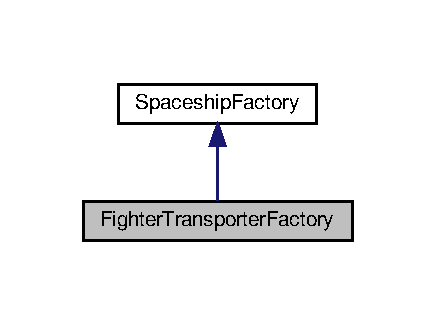
\includegraphics[width=209pt]{classFighterTransporterFactory__inherit__graph}
\end{center}
\end{figure}


Collaboration diagram for Fighter\+Transporter\+Factory\+:\nopagebreak
\begin{figure}[H]
\begin{center}
\leavevmode
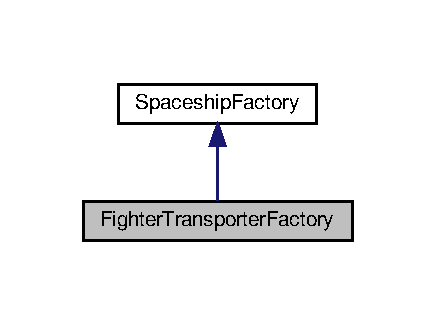
\includegraphics[width=209pt]{classFighterTransporterFactory__coll__graph}
\end{center}
\end{figure}
\subsection*{Public Member Functions}
\begin{DoxyCompactItemize}
\item 
\hyperlink{classFighterTransporterFactory_a6491bf6c6026a412f38df451c0ba7899}{Fighter\+Transporter\+Factory} ()
\item 
\hyperlink{classFighterTransporterFactory_a1ed7e181f7c2ecbfc7b7e69c1085637f}{$\sim$\+Fighter\+Transporter\+Factory} ()
\item 
\hyperlink{classSpaceship}{Spaceship} $\ast$ \hyperlink{classFighterTransporterFactory_a1f2a5002cb9ea812fee8d224884fbdff}{space\+Ship\+Factory\+Method} (string)
\end{DoxyCompactItemize}


\subsection{Detailed Description}
\hyperlink{classFighter}{Fighter} Transporter Factory class. 

\subsection{Constructor \& Destructor Documentation}
\mbox{\Hypertarget{classFighterTransporterFactory_a6491bf6c6026a412f38df451c0ba7899}\label{classFighterTransporterFactory_a6491bf6c6026a412f38df451c0ba7899}} 
\index{Fighter\+Transporter\+Factory@{Fighter\+Transporter\+Factory}!Fighter\+Transporter\+Factory@{Fighter\+Transporter\+Factory}}
\index{Fighter\+Transporter\+Factory@{Fighter\+Transporter\+Factory}!Fighter\+Transporter\+Factory@{Fighter\+Transporter\+Factory}}
\subsubsection{\texorpdfstring{Fighter\+Transporter\+Factory()}{FighterTransporterFactory()}}
{\footnotesize\ttfamily Fighter\+Transporter\+Factory\+::\+Fighter\+Transporter\+Factory (\begin{DoxyParamCaption}{ }\end{DoxyParamCaption})}

Defualt constructor \mbox{\Hypertarget{classFighterTransporterFactory_a1ed7e181f7c2ecbfc7b7e69c1085637f}\label{classFighterTransporterFactory_a1ed7e181f7c2ecbfc7b7e69c1085637f}} 
\index{Fighter\+Transporter\+Factory@{Fighter\+Transporter\+Factory}!````~Fighter\+Transporter\+Factory@{$\sim$\+Fighter\+Transporter\+Factory}}
\index{````~Fighter\+Transporter\+Factory@{$\sim$\+Fighter\+Transporter\+Factory}!Fighter\+Transporter\+Factory@{Fighter\+Transporter\+Factory}}
\subsubsection{\texorpdfstring{$\sim$\+Fighter\+Transporter\+Factory()}{~FighterTransporterFactory()}}
{\footnotesize\ttfamily Fighter\+Transporter\+Factory\+::$\sim$\+Fighter\+Transporter\+Factory (\begin{DoxyParamCaption}{ }\end{DoxyParamCaption})}

Default desctructor 

\subsection{Member Function Documentation}
\mbox{\Hypertarget{classFighterTransporterFactory_a1f2a5002cb9ea812fee8d224884fbdff}\label{classFighterTransporterFactory_a1f2a5002cb9ea812fee8d224884fbdff}} 
\index{Fighter\+Transporter\+Factory@{Fighter\+Transporter\+Factory}!space\+Ship\+Factory\+Method@{space\+Ship\+Factory\+Method}}
\index{space\+Ship\+Factory\+Method@{space\+Ship\+Factory\+Method}!Fighter\+Transporter\+Factory@{Fighter\+Transporter\+Factory}}
\subsubsection{\texorpdfstring{space\+Ship\+Factory\+Method()}{spaceShipFactoryMethod()}}
{\footnotesize\ttfamily \hyperlink{classSpaceship}{Spaceship} $\ast$ Fighter\+Transporter\+Factory\+::space\+Ship\+Factory\+Method (\begin{DoxyParamCaption}\item[{string}]{n }\end{DoxyParamCaption})\hspace{0.3cm}{\ttfamily [virtual]}}

Method to create \hyperlink{classFighterTransporter}{Fighter\+Transporter}\textquotesingle{}s \begin{DoxyReturn}{Returns}
newly created spaceship 
\end{DoxyReturn}


Implements \hyperlink{classSpaceshipFactory_a70b50dd616cb16f50088eff9ca07cda9}{Spaceship\+Factory}.



The documentation for this class was generated from the following files\+:\begin{DoxyCompactItemize}
\item 
Fighter\+Transporter\+Factory.\+h\item 
Fighter\+Transporter\+Factory.\+cpp\end{DoxyCompactItemize}

\hypertarget{classFrigate}{}\section{Frigate Class Reference}
\label{classFrigate}\index{Frigate@{Frigate}}


\hyperlink{classFrigate}{Frigate} class.  




{\ttfamily \#include $<$Frigate.\+h$>$}



Inheritance diagram for Frigate\+:
% FIG 0


Collaboration diagram for Frigate\+:
% FIG 1
\subsection*{Public Member Functions}
\begin{DoxyCompactItemize}
\item 
\hyperlink{classFrigate_ad68c1d421cc3872688a19727055632a2}{Frigate} ()
\item 
\hyperlink{classFrigate_a86559f40e7725443c89039ee623fab2b}{$\sim$\+Frigate} ()
\item 
virtual void \hyperlink{classFrigate_ae06208eed84e006385e4d337e1f04c7d}{add\+Component} (\hyperlink{classSpaceship}{Spaceship} $\ast$)
\end{DoxyCompactItemize}


\subsection{Detailed Description}
\hyperlink{classFrigate}{Frigate} class. 

\subsection{Constructor \& Destructor Documentation}
\mbox{\Hypertarget{classFrigate_ad68c1d421cc3872688a19727055632a2}\label{classFrigate_ad68c1d421cc3872688a19727055632a2}} 
\index{Frigate@{Frigate}!Frigate@{Frigate}}
\index{Frigate@{Frigate}!Frigate@{Frigate}}
\subsubsection{\texorpdfstring{Frigate()}{Frigate()}}
{\footnotesize\ttfamily Frigate\+::\+Frigate (\begin{DoxyParamCaption}{ }\end{DoxyParamCaption})\hspace{0.3cm}{\ttfamily [inline]}}

Default constructor \mbox{\Hypertarget{classFrigate_a86559f40e7725443c89039ee623fab2b}\label{classFrigate_a86559f40e7725443c89039ee623fab2b}} 
\index{Frigate@{Frigate}!````~Frigate@{$\sim$\+Frigate}}
\index{````~Frigate@{$\sim$\+Frigate}!Frigate@{Frigate}}
\subsubsection{\texorpdfstring{$\sim$\+Frigate()}{~Frigate()}}
{\footnotesize\ttfamily Frigate\+::$\sim$\+Frigate (\begin{DoxyParamCaption}{ }\end{DoxyParamCaption})\hspace{0.3cm}{\ttfamily [inline]}}

Default desctructor 

\subsection{Member Function Documentation}
\mbox{\Hypertarget{classFrigate_ae06208eed84e006385e4d337e1f04c7d}\label{classFrigate_ae06208eed84e006385e4d337e1f04c7d}} 
\index{Frigate@{Frigate}!add\+Component@{add\+Component}}
\index{add\+Component@{add\+Component}!Frigate@{Frigate}}
\subsubsection{\texorpdfstring{add\+Component()}{addComponent()}}
{\footnotesize\ttfamily virtual void Frigate\+::add\+Component (\begin{DoxyParamCaption}\item[{\hyperlink{classSpaceship}{Spaceship} $\ast$}]{ }\end{DoxyParamCaption})\hspace{0.3cm}{\ttfamily [inline]}, {\ttfamily [virtual]}}

Add a component to the spaceship 
\begin{DoxyParams}{Parameters}
{\em s} & -\/ component being added \\
\hline
\end{DoxyParams}


Implements \hyperlink{classSpaceship_ac1b4673a691cd100708ddea08cd9f192}{Spaceship}.



The documentation for this class was generated from the following file\+:\begin{DoxyCompactItemize}
\item 
Frigate.\+h\end{DoxyCompactItemize}

\hypertarget{classFrigateFactory}{}\section{Frigate\+Factory Class Reference}
\label{classFrigateFactory}\index{Frigate\+Factory@{Frigate\+Factory}}


\hyperlink{classFrigate}{Frigate} Factory class.  




{\ttfamily \#include $<$Frigate\+Factory.\+h$>$}



Inheritance diagram for Frigate\+Factory\+:
% FIG 0


Collaboration diagram for Frigate\+Factory\+:
% FIG 1
\subsection*{Public Member Functions}
\begin{DoxyCompactItemize}
\item 
\hyperlink{classFrigateFactory_a1025a996e1e48f03bacac243ec1540b8}{Frigate\+Factory} ()
\item 
\hyperlink{classFrigateFactory_ae1433ffe26d615f35bf62d00c026c6a9}{$\sim$\+Frigate\+Factory} ()
\item 
\hyperlink{classSpaceship}{Spaceship} $\ast$ \hyperlink{classFrigateFactory_adfe55ec4fd28b09ab5f0bba3e782c87d}{space\+Ship\+Factory\+Method} ()
\end{DoxyCompactItemize}


\subsection{Detailed Description}
\hyperlink{classFrigate}{Frigate} Factory class. 

\subsection{Constructor \& Destructor Documentation}
\mbox{\Hypertarget{classFrigateFactory_a1025a996e1e48f03bacac243ec1540b8}\label{classFrigateFactory_a1025a996e1e48f03bacac243ec1540b8}} 
\index{Frigate\+Factory@{Frigate\+Factory}!Frigate\+Factory@{Frigate\+Factory}}
\index{Frigate\+Factory@{Frigate\+Factory}!Frigate\+Factory@{Frigate\+Factory}}
\subsubsection{\texorpdfstring{Frigate\+Factory()}{FrigateFactory()}}
{\footnotesize\ttfamily Frigate\+Factory\+::\+Frigate\+Factory (\begin{DoxyParamCaption}{ }\end{DoxyParamCaption})}

Default Constructor \mbox{\Hypertarget{classFrigateFactory_ae1433ffe26d615f35bf62d00c026c6a9}\label{classFrigateFactory_ae1433ffe26d615f35bf62d00c026c6a9}} 
\index{Frigate\+Factory@{Frigate\+Factory}!````~Frigate\+Factory@{$\sim$\+Frigate\+Factory}}
\index{````~Frigate\+Factory@{$\sim$\+Frigate\+Factory}!Frigate\+Factory@{Frigate\+Factory}}
\subsubsection{\texorpdfstring{$\sim$\+Frigate\+Factory()}{~FrigateFactory()}}
{\footnotesize\ttfamily Frigate\+Factory\+::$\sim$\+Frigate\+Factory (\begin{DoxyParamCaption}{ }\end{DoxyParamCaption})}

Default desctructor 

\subsection{Member Function Documentation}
\mbox{\Hypertarget{classFrigateFactory_adfe55ec4fd28b09ab5f0bba3e782c87d}\label{classFrigateFactory_adfe55ec4fd28b09ab5f0bba3e782c87d}} 
\index{Frigate\+Factory@{Frigate\+Factory}!space\+Ship\+Factory\+Method@{space\+Ship\+Factory\+Method}}
\index{space\+Ship\+Factory\+Method@{space\+Ship\+Factory\+Method}!Frigate\+Factory@{Frigate\+Factory}}
\subsubsection{\texorpdfstring{space\+Ship\+Factory\+Method()}{spaceShipFactoryMethod()}}
{\footnotesize\ttfamily \hyperlink{classSpaceship}{Spaceship} $\ast$ Frigate\+Factory\+::space\+Ship\+Factory\+Method (\begin{DoxyParamCaption}{ }\end{DoxyParamCaption})\hspace{0.3cm}{\ttfamily [virtual]}}

Method to create \hyperlink{classFrigate}{Frigate}\textquotesingle{}s \begin{DoxyReturn}{Returns}
newly created ship 
\end{DoxyReturn}


Reimplemented from \hyperlink{classSpaceshipFactory_a146f5e82385a55e9bf4ce63e28f99a9d}{Spaceship\+Factory}.



The documentation for this class was generated from the following files\+:\begin{DoxyCompactItemize}
\item 
Frigate\+Factory.\+h\item 
Frigate\+Factory.\+cpp\end{DoxyCompactItemize}

\hypertarget{classInvade}{}\section{Invade Class Reference}
\label{classInvade}\index{Invade@{Invade}}


\hyperlink{classPlanet}{Planet} class.  




{\ttfamily \#include $<$Invade.\+h$>$}



Inheritance diagram for Invade\+:\nopagebreak
\begin{figure}[H]
\begin{center}
\leavevmode
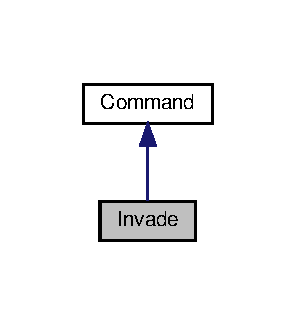
\includegraphics[width=142pt]{classInvade__inherit__graph}
\end{center}
\end{figure}


Collaboration diagram for Invade\+:\nopagebreak
\begin{figure}[H]
\begin{center}
\leavevmode
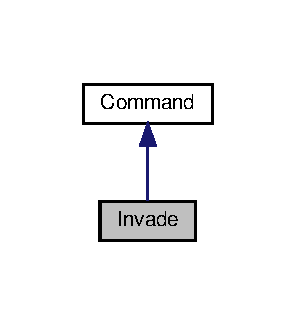
\includegraphics[width=142pt]{classInvade__coll__graph}
\end{center}
\end{figure}
\subsection*{Public Member Functions}
\begin{DoxyCompactItemize}
\item 
\hyperlink{classInvade_a7abfb047bd3df1e5d44a0c65701b58bd}{Invade} ()
\item 
void \hyperlink{classInvade_a111ebe8b6c5a3646b697ca906c815b35}{execute} ()
\item 
\hyperlink{classInvade_a54e5cbe56b8748809beda7d798546103}{$\sim$\+Invade} ()
\item 
\hyperlink{classInvade_a5fdc8e1f96494355363666c6ef5a4fac}{Invade} (\hyperlink{classSpaceship}{Spaceship} $\ast$ship)
\end{DoxyCompactItemize}


\subsection{Detailed Description}
\hyperlink{classPlanet}{Planet} class. 

\subsection{Constructor \& Destructor Documentation}
\mbox{\Hypertarget{classInvade_a7abfb047bd3df1e5d44a0c65701b58bd}\label{classInvade_a7abfb047bd3df1e5d44a0c65701b58bd}} 
\index{Invade@{Invade}!Invade@{Invade}}
\index{Invade@{Invade}!Invade@{Invade}}
\subsubsection{\texorpdfstring{Invade()}{Invade()}\hspace{0.1cm}{\footnotesize\ttfamily [1/2]}}
{\footnotesize\ttfamily Invade\+::\+Invade (\begin{DoxyParamCaption}{ }\end{DoxyParamCaption})}

default constructor \mbox{\Hypertarget{classInvade_a54e5cbe56b8748809beda7d798546103}\label{classInvade_a54e5cbe56b8748809beda7d798546103}} 
\index{Invade@{Invade}!````~Invade@{$\sim$\+Invade}}
\index{````~Invade@{$\sim$\+Invade}!Invade@{Invade}}
\subsubsection{\texorpdfstring{$\sim$\+Invade()}{~Invade()}}
{\footnotesize\ttfamily Invade\+::$\sim$\+Invade (\begin{DoxyParamCaption}{ }\end{DoxyParamCaption})}

Default Destructor \mbox{\Hypertarget{classInvade_a5fdc8e1f96494355363666c6ef5a4fac}\label{classInvade_a5fdc8e1f96494355363666c6ef5a4fac}} 
\index{Invade@{Invade}!Invade@{Invade}}
\index{Invade@{Invade}!Invade@{Invade}}
\subsubsection{\texorpdfstring{Invade()}{Invade()}\hspace{0.1cm}{\footnotesize\ttfamily [2/2]}}
{\footnotesize\ttfamily Invade\+::\+Invade (\begin{DoxyParamCaption}\item[{\hyperlink{classSpaceship}{Spaceship} $\ast$}]{ship }\end{DoxyParamCaption})\hspace{0.3cm}{\ttfamily [inline]}}

Paramaterised constructor 
\begin{DoxyParams}{Parameters}
{\em ship} & \\
\hline
\end{DoxyParams}


\subsection{Member Function Documentation}
\mbox{\Hypertarget{classInvade_a111ebe8b6c5a3646b697ca906c815b35}\label{classInvade_a111ebe8b6c5a3646b697ca906c815b35}} 
\index{Invade@{Invade}!execute@{execute}}
\index{execute@{execute}!Invade@{Invade}}
\subsubsection{\texorpdfstring{execute()}{execute()}}
{\footnotesize\ttfamily void Invade\+::execute (\begin{DoxyParamCaption}{ }\end{DoxyParamCaption})\hspace{0.3cm}{\ttfamily [virtual]}}

Execute Function That will call The Receivers action function 

Implements \hyperlink{classCommand_a6fd7d9bd8df8bfc881e4d6c7cd1878b7}{Command}.



The documentation for this class was generated from the following files\+:\begin{DoxyCompactItemize}
\item 
Invade.\+h\item 
Invade.\+cpp\end{DoxyCompactItemize}

\hypertarget{classLevelOneThreat}{}\section{Level\+One\+Threat Class Reference}
\label{classLevelOneThreat}\index{Level\+One\+Threat@{Level\+One\+Threat}}


Level One Threat class.  




{\ttfamily \#include $<$Level\+One.\+h$>$}



Inheritance diagram for Level\+One\+Threat\+:
% FIG 0


Collaboration diagram for Level\+One\+Threat\+:
% FIG 1
\subsection*{Public Member Functions}
\begin{DoxyCompactItemize}
\item 
\hyperlink{classLevelOneThreat_ae90b42ebcce70476ff405ccdcde0627e}{Level\+One\+Threat} ()
\item 
\hyperlink{classLevelOneThreat_a1c6e77c98473057eef8fe66f0e325fcf}{$\sim$\+Level\+One\+Threat} ()
\item 
\hyperlink{classThreatLevel}{Threat\+Level} $\ast$ \hyperlink{classLevelOneThreat_afc68f742f1101cb8d533d8cec21bac3f}{increase\+Threat\+Level} ()
\item 
\hyperlink{classThreatLevel}{Threat\+Level} $\ast$ \hyperlink{classLevelOneThreat_a9a2899ac02e075905671ea03374cd561}{decrease\+Threat\+Level} ()
\item 
void \hyperlink{classLevelOneThreat_a902492d8341a398b0209fb89e2aca68e}{print} ()
\end{DoxyCompactItemize}


\subsection{Detailed Description}
Level One Threat class. 

\subsection{Constructor \& Destructor Documentation}
\mbox{\Hypertarget{classLevelOneThreat_ae90b42ebcce70476ff405ccdcde0627e}\label{classLevelOneThreat_ae90b42ebcce70476ff405ccdcde0627e}} 
\index{Level\+One\+Threat@{Level\+One\+Threat}!Level\+One\+Threat@{Level\+One\+Threat}}
\index{Level\+One\+Threat@{Level\+One\+Threat}!Level\+One\+Threat@{Level\+One\+Threat}}
\subsubsection{\texorpdfstring{Level\+One\+Threat()}{LevelOneThreat()}}
{\footnotesize\ttfamily Level\+One\+Threat\+::\+Level\+One\+Threat (\begin{DoxyParamCaption}{ }\end{DoxyParamCaption})}

Default contructor \mbox{\Hypertarget{classLevelOneThreat_a1c6e77c98473057eef8fe66f0e325fcf}\label{classLevelOneThreat_a1c6e77c98473057eef8fe66f0e325fcf}} 
\index{Level\+One\+Threat@{Level\+One\+Threat}!````~Level\+One\+Threat@{$\sim$\+Level\+One\+Threat}}
\index{````~Level\+One\+Threat@{$\sim$\+Level\+One\+Threat}!Level\+One\+Threat@{Level\+One\+Threat}}
\subsubsection{\texorpdfstring{$\sim$\+Level\+One\+Threat()}{~LevelOneThreat()}}
{\footnotesize\ttfamily Level\+One\+Threat\+::$\sim$\+Level\+One\+Threat (\begin{DoxyParamCaption}{ }\end{DoxyParamCaption})}

Default desctructor 

\subsection{Member Function Documentation}
\mbox{\Hypertarget{classLevelOneThreat_a9a2899ac02e075905671ea03374cd561}\label{classLevelOneThreat_a9a2899ac02e075905671ea03374cd561}} 
\index{Level\+One\+Threat@{Level\+One\+Threat}!decrease\+Threat\+Level@{decrease\+Threat\+Level}}
\index{decrease\+Threat\+Level@{decrease\+Threat\+Level}!Level\+One\+Threat@{Level\+One\+Threat}}
\subsubsection{\texorpdfstring{decrease\+Threat\+Level()}{decreaseThreatLevel()}}
{\footnotesize\ttfamily \hyperlink{classThreatLevel}{Threat\+Level} $\ast$ Level\+One\+Threat\+::decrease\+Threat\+Level (\begin{DoxyParamCaption}{ }\end{DoxyParamCaption})\hspace{0.3cm}{\ttfamily [virtual]}}

Decrase the threat level \begin{DoxyReturn}{Returns}
new threat level 
\end{DoxyReturn}


Reimplemented from \hyperlink{classThreatLevel_a3545ec161fbe4c01beafb9b43624c7e8}{Threat\+Level}.

\mbox{\Hypertarget{classLevelOneThreat_afc68f742f1101cb8d533d8cec21bac3f}\label{classLevelOneThreat_afc68f742f1101cb8d533d8cec21bac3f}} 
\index{Level\+One\+Threat@{Level\+One\+Threat}!increase\+Threat\+Level@{increase\+Threat\+Level}}
\index{increase\+Threat\+Level@{increase\+Threat\+Level}!Level\+One\+Threat@{Level\+One\+Threat}}
\subsubsection{\texorpdfstring{increase\+Threat\+Level()}{increaseThreatLevel()}}
{\footnotesize\ttfamily \hyperlink{classThreatLevel}{Threat\+Level} $\ast$ Level\+One\+Threat\+::increase\+Threat\+Level (\begin{DoxyParamCaption}{ }\end{DoxyParamCaption})\hspace{0.3cm}{\ttfamily [virtual]}}

Increase the threat level \begin{DoxyReturn}{Returns}
the new threat level 
\end{DoxyReturn}


Reimplemented from \hyperlink{classThreatLevel_ae18f6ebe2186ae1b61d4817196f969e3}{Threat\+Level}.

\mbox{\Hypertarget{classLevelOneThreat_a902492d8341a398b0209fb89e2aca68e}\label{classLevelOneThreat_a902492d8341a398b0209fb89e2aca68e}} 
\index{Level\+One\+Threat@{Level\+One\+Threat}!print@{print}}
\index{print@{print}!Level\+One\+Threat@{Level\+One\+Threat}}
\subsubsection{\texorpdfstring{print()}{print()}}
{\footnotesize\ttfamily void Level\+One\+Threat\+::print (\begin{DoxyParamCaption}{ }\end{DoxyParamCaption})\hspace{0.3cm}{\ttfamily [virtual]}}

Print the current threat level 

Reimplemented from \hyperlink{classThreatLevel_a5bdff5eeffed8db616ca06091097c138}{Threat\+Level}.



The documentation for this class was generated from the following files\+:\begin{DoxyCompactItemize}
\item 
Level\+One.\+h\item 
Level\+One.\+cpp\end{DoxyCompactItemize}

\hypertarget{classLevelThreeThreat}{}\section{Level\+Three\+Threat Class Reference}
\label{classLevelThreeThreat}\index{Level\+Three\+Threat@{Level\+Three\+Threat}}


Level Three Threat class.  




{\ttfamily \#include $<$Level\+Three.\+h$>$}



Inheritance diagram for Level\+Three\+Threat\+:
% FIG 0


Collaboration diagram for Level\+Three\+Threat\+:
% FIG 1
\subsection*{Public Member Functions}
\begin{DoxyCompactItemize}
\item 
\hyperlink{classLevelThreeThreat_a5c9b00bc5cd2459c7b1adf2542afc702}{Level\+Three\+Threat} ()
\item 
\hyperlink{classLevelThreeThreat_ab5caa48c8913099e0a3520ce6849b295}{$\sim$\+Level\+Three\+Threat} ()
\item 
\hyperlink{classThreatLevel}{Threat\+Level} $\ast$ \hyperlink{classLevelThreeThreat_a284c2b79a9a85f5e164f15c258c6e9ca}{increase\+Threat\+Level} ()
\item 
\hyperlink{classThreatLevel}{Threat\+Level} $\ast$ \hyperlink{classLevelThreeThreat_a98337ab08fe61b136d9c9e48f7ace804}{decrease\+Threat\+Level} ()
\item 
void \hyperlink{classLevelThreeThreat_a3bdd7e61f3938123ce9c705623e0d98a}{print} ()
\end{DoxyCompactItemize}


\subsection{Detailed Description}
Level Three Threat class. 

\subsection{Constructor \& Destructor Documentation}
\mbox{\Hypertarget{classLevelThreeThreat_a5c9b00bc5cd2459c7b1adf2542afc702}\label{classLevelThreeThreat_a5c9b00bc5cd2459c7b1adf2542afc702}} 
\index{Level\+Three\+Threat@{Level\+Three\+Threat}!Level\+Three\+Threat@{Level\+Three\+Threat}}
\index{Level\+Three\+Threat@{Level\+Three\+Threat}!Level\+Three\+Threat@{Level\+Three\+Threat}}
\subsubsection{\texorpdfstring{Level\+Three\+Threat()}{LevelThreeThreat()}}
{\footnotesize\ttfamily Level\+Three\+Threat\+::\+Level\+Three\+Threat (\begin{DoxyParamCaption}{ }\end{DoxyParamCaption})}

Default constructor \mbox{\Hypertarget{classLevelThreeThreat_ab5caa48c8913099e0a3520ce6849b295}\label{classLevelThreeThreat_ab5caa48c8913099e0a3520ce6849b295}} 
\index{Level\+Three\+Threat@{Level\+Three\+Threat}!````~Level\+Three\+Threat@{$\sim$\+Level\+Three\+Threat}}
\index{````~Level\+Three\+Threat@{$\sim$\+Level\+Three\+Threat}!Level\+Three\+Threat@{Level\+Three\+Threat}}
\subsubsection{\texorpdfstring{$\sim$\+Level\+Three\+Threat()}{~LevelThreeThreat()}}
{\footnotesize\ttfamily Level\+Three\+Threat\+::$\sim$\+Level\+Three\+Threat (\begin{DoxyParamCaption}{ }\end{DoxyParamCaption})}

Default desctructor 

\subsection{Member Function Documentation}
\mbox{\Hypertarget{classLevelThreeThreat_a98337ab08fe61b136d9c9e48f7ace804}\label{classLevelThreeThreat_a98337ab08fe61b136d9c9e48f7ace804}} 
\index{Level\+Three\+Threat@{Level\+Three\+Threat}!decrease\+Threat\+Level@{decrease\+Threat\+Level}}
\index{decrease\+Threat\+Level@{decrease\+Threat\+Level}!Level\+Three\+Threat@{Level\+Three\+Threat}}
\subsubsection{\texorpdfstring{decrease\+Threat\+Level()}{decreaseThreatLevel()}}
{\footnotesize\ttfamily \hyperlink{classThreatLevel}{Threat\+Level} $\ast$ Level\+Three\+Threat\+::decrease\+Threat\+Level (\begin{DoxyParamCaption}{ }\end{DoxyParamCaption})\hspace{0.3cm}{\ttfamily [virtual]}}

Decrease threat level \begin{DoxyReturn}{Returns}
new threat level 
\end{DoxyReturn}


Reimplemented from \hyperlink{classThreatLevel_a3545ec161fbe4c01beafb9b43624c7e8}{Threat\+Level}.

\mbox{\Hypertarget{classLevelThreeThreat_a284c2b79a9a85f5e164f15c258c6e9ca}\label{classLevelThreeThreat_a284c2b79a9a85f5e164f15c258c6e9ca}} 
\index{Level\+Three\+Threat@{Level\+Three\+Threat}!increase\+Threat\+Level@{increase\+Threat\+Level}}
\index{increase\+Threat\+Level@{increase\+Threat\+Level}!Level\+Three\+Threat@{Level\+Three\+Threat}}
\subsubsection{\texorpdfstring{increase\+Threat\+Level()}{increaseThreatLevel()}}
{\footnotesize\ttfamily \hyperlink{classThreatLevel}{Threat\+Level} $\ast$ Level\+Three\+Threat\+::increase\+Threat\+Level (\begin{DoxyParamCaption}{ }\end{DoxyParamCaption})\hspace{0.3cm}{\ttfamily [virtual]}}

Increase threat level \begin{DoxyReturn}{Returns}
new threat level 
\end{DoxyReturn}


Reimplemented from \hyperlink{classThreatLevel_ae18f6ebe2186ae1b61d4817196f969e3}{Threat\+Level}.

\mbox{\Hypertarget{classLevelThreeThreat_a3bdd7e61f3938123ce9c705623e0d98a}\label{classLevelThreeThreat_a3bdd7e61f3938123ce9c705623e0d98a}} 
\index{Level\+Three\+Threat@{Level\+Three\+Threat}!print@{print}}
\index{print@{print}!Level\+Three\+Threat@{Level\+Three\+Threat}}
\subsubsection{\texorpdfstring{print()}{print()}}
{\footnotesize\ttfamily void Level\+Three\+Threat\+::print (\begin{DoxyParamCaption}{ }\end{DoxyParamCaption})\hspace{0.3cm}{\ttfamily [virtual]}}

Print current threat level 

Reimplemented from \hyperlink{classThreatLevel_a5bdff5eeffed8db616ca06091097c138}{Threat\+Level}.



The documentation for this class was generated from the following files\+:\begin{DoxyCompactItemize}
\item 
Level\+Three.\+h\item 
Level\+Three.\+cpp\end{DoxyCompactItemize}

\hypertarget{classLevelTwoThreat}{}\section{Level\+Two\+Threat Class Reference}
\label{classLevelTwoThreat}\index{Level\+Two\+Threat@{Level\+Two\+Threat}}


Level Two Threat class.  




{\ttfamily \#include $<$Level\+Two.\+h$>$}



Inheritance diagram for Level\+Two\+Threat\+:\nopagebreak
\begin{figure}[H]
\begin{center}
\leavevmode
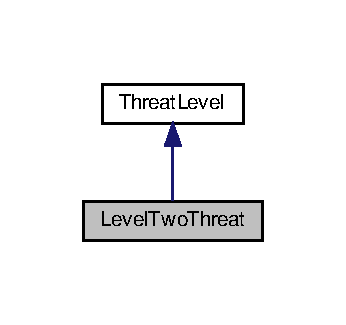
\includegraphics[width=166pt]{classLevelTwoThreat__inherit__graph}
\end{center}
\end{figure}


Collaboration diagram for Level\+Two\+Threat\+:\nopagebreak
\begin{figure}[H]
\begin{center}
\leavevmode
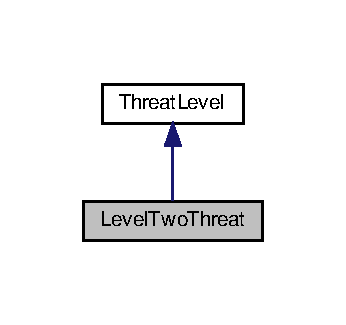
\includegraphics[width=166pt]{classLevelTwoThreat__coll__graph}
\end{center}
\end{figure}
\subsection*{Public Member Functions}
\begin{DoxyCompactItemize}
\item 
\hyperlink{classLevelTwoThreat_a862bf482af05fb712da3f02564653ee1}{Level\+Two\+Threat} ()
\item 
\hyperlink{classLevelTwoThreat_af07b8e6bfd18b564a83c41cae1ffb37a}{$\sim$\+Level\+Two\+Threat} ()
\item 
\hyperlink{classThreatLevel}{Threat\+Level} $\ast$ \hyperlink{classLevelTwoThreat_a54b4d396cdd27504f1a8063c04be5bcf}{increase\+Threat\+Level} ()
\item 
\hyperlink{classThreatLevel}{Threat\+Level} $\ast$ \hyperlink{classLevelTwoThreat_a1d9e88b0f43396721a2f51ae67191359}{decrease\+Threat\+Level} ()
\item 
void \hyperlink{classLevelTwoThreat_a9e21bc1a55bb25d86346c484f5fd0525}{print} ()
\end{DoxyCompactItemize}


\subsection{Detailed Description}
Level Two Threat class. 

\subsection{Constructor \& Destructor Documentation}
\mbox{\Hypertarget{classLevelTwoThreat_a862bf482af05fb712da3f02564653ee1}\label{classLevelTwoThreat_a862bf482af05fb712da3f02564653ee1}} 
\index{Level\+Two\+Threat@{Level\+Two\+Threat}!Level\+Two\+Threat@{Level\+Two\+Threat}}
\index{Level\+Two\+Threat@{Level\+Two\+Threat}!Level\+Two\+Threat@{Level\+Two\+Threat}}
\subsubsection{\texorpdfstring{Level\+Two\+Threat()}{LevelTwoThreat()}}
{\footnotesize\ttfamily Level\+Two\+Threat\+::\+Level\+Two\+Threat (\begin{DoxyParamCaption}{ }\end{DoxyParamCaption})}

Default constructor \mbox{\Hypertarget{classLevelTwoThreat_af07b8e6bfd18b564a83c41cae1ffb37a}\label{classLevelTwoThreat_af07b8e6bfd18b564a83c41cae1ffb37a}} 
\index{Level\+Two\+Threat@{Level\+Two\+Threat}!````~Level\+Two\+Threat@{$\sim$\+Level\+Two\+Threat}}
\index{````~Level\+Two\+Threat@{$\sim$\+Level\+Two\+Threat}!Level\+Two\+Threat@{Level\+Two\+Threat}}
\subsubsection{\texorpdfstring{$\sim$\+Level\+Two\+Threat()}{~LevelTwoThreat()}}
{\footnotesize\ttfamily Level\+Two\+Threat\+::$\sim$\+Level\+Two\+Threat (\begin{DoxyParamCaption}{ }\end{DoxyParamCaption})}

Default destructor 

\subsection{Member Function Documentation}
\mbox{\Hypertarget{classLevelTwoThreat_a1d9e88b0f43396721a2f51ae67191359}\label{classLevelTwoThreat_a1d9e88b0f43396721a2f51ae67191359}} 
\index{Level\+Two\+Threat@{Level\+Two\+Threat}!decrease\+Threat\+Level@{decrease\+Threat\+Level}}
\index{decrease\+Threat\+Level@{decrease\+Threat\+Level}!Level\+Two\+Threat@{Level\+Two\+Threat}}
\subsubsection{\texorpdfstring{decrease\+Threat\+Level()}{decreaseThreatLevel()}}
{\footnotesize\ttfamily \hyperlink{classThreatLevel}{Threat\+Level} $\ast$ Level\+Two\+Threat\+::decrease\+Threat\+Level (\begin{DoxyParamCaption}{ }\end{DoxyParamCaption})\hspace{0.3cm}{\ttfamily [virtual]}}

Decrase threat level \begin{DoxyReturn}{Returns}
new threat level 
\end{DoxyReturn}


Reimplemented from \hyperlink{classThreatLevel_a3545ec161fbe4c01beafb9b43624c7e8}{Threat\+Level}.

\mbox{\Hypertarget{classLevelTwoThreat_a54b4d396cdd27504f1a8063c04be5bcf}\label{classLevelTwoThreat_a54b4d396cdd27504f1a8063c04be5bcf}} 
\index{Level\+Two\+Threat@{Level\+Two\+Threat}!increase\+Threat\+Level@{increase\+Threat\+Level}}
\index{increase\+Threat\+Level@{increase\+Threat\+Level}!Level\+Two\+Threat@{Level\+Two\+Threat}}
\subsubsection{\texorpdfstring{increase\+Threat\+Level()}{increaseThreatLevel()}}
{\footnotesize\ttfamily \hyperlink{classThreatLevel}{Threat\+Level} $\ast$ Level\+Two\+Threat\+::increase\+Threat\+Level (\begin{DoxyParamCaption}{ }\end{DoxyParamCaption})\hspace{0.3cm}{\ttfamily [virtual]}}

Increase threat level \begin{DoxyReturn}{Returns}
new threat level 
\end{DoxyReturn}


Reimplemented from \hyperlink{classThreatLevel_ae18f6ebe2186ae1b61d4817196f969e3}{Threat\+Level}.

\mbox{\Hypertarget{classLevelTwoThreat_a9e21bc1a55bb25d86346c484f5fd0525}\label{classLevelTwoThreat_a9e21bc1a55bb25d86346c484f5fd0525}} 
\index{Level\+Two\+Threat@{Level\+Two\+Threat}!print@{print}}
\index{print@{print}!Level\+Two\+Threat@{Level\+Two\+Threat}}
\subsubsection{\texorpdfstring{print()}{print()}}
{\footnotesize\ttfamily void Level\+Two\+Threat\+::print (\begin{DoxyParamCaption}{ }\end{DoxyParamCaption})\hspace{0.3cm}{\ttfamily [virtual]}}

Print threat level 

Reimplemented from \hyperlink{classThreatLevel_a5bdff5eeffed8db616ca06091097c138}{Threat\+Level}.



The documentation for this class was generated from the following files\+:\begin{DoxyCompactItemize}
\item 
Level\+Two.\+h\item 
Level\+Two.\+cpp\end{DoxyCompactItemize}

\hypertarget{classMemento}{}\section{Memento Class Reference}
\label{classMemento}\index{Memento@{Memento}}


\hyperlink{classMemento}{Memento} class.  




{\ttfamily \#include $<$Memento.\+h$>$}

\subsection*{Public Member Functions}
\begin{DoxyCompactItemize}
\item 
virtual \hyperlink{classMemento_af680b5488989567d0f03d655c4232924}{$\sim$\+Memento} ()
\end{DoxyCompactItemize}
\subsection*{Friends}
\begin{DoxyCompactItemize}
\item 
\mbox{\Hypertarget{classMemento_a35831582729e6f468d0640f39619f09e}\label{classMemento_a35831582729e6f468d0640f39619f09e}} 
class {\bfseries Transport\+Bay}
\end{DoxyCompactItemize}


\subsection{Detailed Description}
\hyperlink{classMemento}{Memento} class. 

\subsection{Constructor \& Destructor Documentation}
\mbox{\Hypertarget{classMemento_af680b5488989567d0f03d655c4232924}\label{classMemento_af680b5488989567d0f03d655c4232924}} 
\index{Memento@{Memento}!````~Memento@{$\sim$\+Memento}}
\index{````~Memento@{$\sim$\+Memento}!Memento@{Memento}}
\subsubsection{\texorpdfstring{$\sim$\+Memento()}{~Memento()}}
{\footnotesize\ttfamily Memento\+::$\sim$\+Memento (\begin{DoxyParamCaption}{ }\end{DoxyParamCaption})\hspace{0.3cm}{\ttfamily [virtual]}}

Virtual default destructor 

The documentation for this class was generated from the following files\+:\begin{DoxyCompactItemize}
\item 
Memento.\+h\item 
Memento.\+cpp\end{DoxyCompactItemize}

\hypertarget{classMine}{}\section{Mine Class Reference}
\label{classMine}\index{Mine@{Mine}}


\hyperlink{classPlanet}{Planet} class.  




{\ttfamily \#include $<$Mine.\+h$>$}



Inheritance diagram for Mine\+:\nopagebreak
\begin{figure}[H]
\begin{center}
\leavevmode
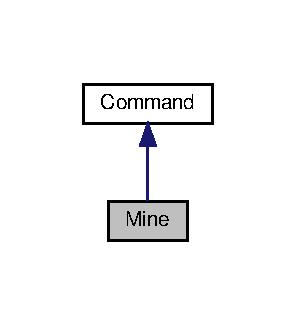
\includegraphics[width=142pt]{classMine__inherit__graph}
\end{center}
\end{figure}


Collaboration diagram for Mine\+:\nopagebreak
\begin{figure}[H]
\begin{center}
\leavevmode
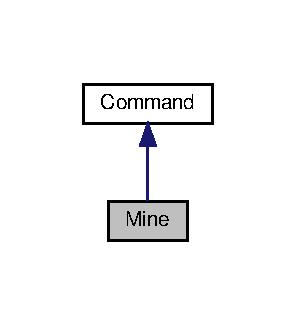
\includegraphics[width=142pt]{classMine__coll__graph}
\end{center}
\end{figure}
\subsection*{Public Member Functions}
\begin{DoxyCompactItemize}
\item 
\hyperlink{classMine_a84f100c1d6797402ab2220d2ad699be2}{Mine} ()
\item 
void \hyperlink{classMine_a2cfa55d098ec47369eed81226d82da25}{execute} ()
\item 
\hyperlink{classMine_abfde171f93b463d81d5b18f767a3a37c}{$\sim$\+Mine} ()
\item 
\hyperlink{classMine_a3a7383f5c2f0f98b7d2c0cb2a9a67073}{Mine} (\hyperlink{classSpaceship}{Spaceship} $\ast$ship)
\end{DoxyCompactItemize}


\subsection{Detailed Description}
\hyperlink{classPlanet}{Planet} class. 

\subsection{Constructor \& Destructor Documentation}
\mbox{\Hypertarget{classMine_a84f100c1d6797402ab2220d2ad699be2}\label{classMine_a84f100c1d6797402ab2220d2ad699be2}} 
\index{Mine@{Mine}!Mine@{Mine}}
\index{Mine@{Mine}!Mine@{Mine}}
\subsubsection{\texorpdfstring{Mine()}{Mine()}\hspace{0.1cm}{\footnotesize\ttfamily [1/2]}}
{\footnotesize\ttfamily Mine\+::\+Mine (\begin{DoxyParamCaption}{ }\end{DoxyParamCaption})}

default constructor \mbox{\Hypertarget{classMine_abfde171f93b463d81d5b18f767a3a37c}\label{classMine_abfde171f93b463d81d5b18f767a3a37c}} 
\index{Mine@{Mine}!````~Mine@{$\sim$\+Mine}}
\index{````~Mine@{$\sim$\+Mine}!Mine@{Mine}}
\subsubsection{\texorpdfstring{$\sim$\+Mine()}{~Mine()}}
{\footnotesize\ttfamily Mine\+::$\sim$\+Mine (\begin{DoxyParamCaption}{ }\end{DoxyParamCaption})}

Default Destructor \mbox{\Hypertarget{classMine_a3a7383f5c2f0f98b7d2c0cb2a9a67073}\label{classMine_a3a7383f5c2f0f98b7d2c0cb2a9a67073}} 
\index{Mine@{Mine}!Mine@{Mine}}
\index{Mine@{Mine}!Mine@{Mine}}
\subsubsection{\texorpdfstring{Mine()}{Mine()}\hspace{0.1cm}{\footnotesize\ttfamily [2/2]}}
{\footnotesize\ttfamily Mine\+::\+Mine (\begin{DoxyParamCaption}\item[{\hyperlink{classSpaceship}{Spaceship} $\ast$}]{ship }\end{DoxyParamCaption})\hspace{0.3cm}{\ttfamily [inline]}}

Paramaterised constructor 
\begin{DoxyParams}{Parameters}
{\em ship} & \\
\hline
\end{DoxyParams}


\subsection{Member Function Documentation}
\mbox{\Hypertarget{classMine_a2cfa55d098ec47369eed81226d82da25}\label{classMine_a2cfa55d098ec47369eed81226d82da25}} 
\index{Mine@{Mine}!execute@{execute}}
\index{execute@{execute}!Mine@{Mine}}
\subsubsection{\texorpdfstring{execute()}{execute()}}
{\footnotesize\ttfamily void Mine\+::execute (\begin{DoxyParamCaption}{ }\end{DoxyParamCaption})\hspace{0.3cm}{\ttfamily [virtual]}}

Execute Function That will call The Receivers action function 

Implements \hyperlink{classCommand_a6fd7d9bd8df8bfc881e4d6c7cd1878b7}{Command}.



The documentation for this class was generated from the following files\+:\begin{DoxyCompactItemize}
\item 
Mine.\+h\item 
Mine.\+cpp\end{DoxyCompactItemize}

\hypertarget{classMiningStrategy}{}\section{Mining\+Strategy Class Reference}
\label{classMiningStrategy}\index{Mining\+Strategy@{Mining\+Strategy}}


\hyperlink{classMiningStrategy}{Mining\+Strategy} class.  




{\ttfamily \#include $<$Mining\+Strategy.\+h$>$}

\subsection*{Public Member Functions}
\begin{DoxyCompactItemize}
\item 
virtual double \hyperlink{classMiningStrategy_ace2ad68881b60573b90921a8087aee75}{execute} (double a, double b)
\item 
\hyperlink{classMiningStrategy_a9d57c0f71bd7bcc4c13360b9406ceb8c}{$\sim$\+Mining\+Strategy} ()
\end{DoxyCompactItemize}


\subsection{Detailed Description}
\hyperlink{classMiningStrategy}{Mining\+Strategy} class. 

\subsection{Constructor \& Destructor Documentation}
\mbox{\Hypertarget{classMiningStrategy_a9d57c0f71bd7bcc4c13360b9406ceb8c}\label{classMiningStrategy_a9d57c0f71bd7bcc4c13360b9406ceb8c}} 
\index{Mining\+Strategy@{Mining\+Strategy}!````~Mining\+Strategy@{$\sim$\+Mining\+Strategy}}
\index{````~Mining\+Strategy@{$\sim$\+Mining\+Strategy}!Mining\+Strategy@{Mining\+Strategy}}
\subsubsection{\texorpdfstring{$\sim$\+Mining\+Strategy()}{~MiningStrategy()}}
{\footnotesize\ttfamily Mining\+Strategy\+::$\sim$\+Mining\+Strategy (\begin{DoxyParamCaption}{ }\end{DoxyParamCaption})}

default destructor 

\subsection{Member Function Documentation}
\mbox{\Hypertarget{classMiningStrategy_ace2ad68881b60573b90921a8087aee75}\label{classMiningStrategy_ace2ad68881b60573b90921a8087aee75}} 
\index{Mining\+Strategy@{Mining\+Strategy}!execute@{execute}}
\index{execute@{execute}!Mining\+Strategy@{Mining\+Strategy}}
\subsubsection{\texorpdfstring{execute()}{execute()}}
{\footnotesize\ttfamily double Mining\+Strategy\+::execute (\begin{DoxyParamCaption}\item[{double}]{a,  }\item[{double}]{b }\end{DoxyParamCaption})\hspace{0.3cm}{\ttfamily [virtual]}}

overloaded execute for mining resources 

The documentation for this class was generated from the following files\+:\begin{DoxyCompactItemize}
\item 
Mining\+Strategy.\+h\item 
Mining\+Strategy.\+cpp\end{DoxyCompactItemize}

\hypertarget{classNavigator}{}\section{Navigator Class Reference}
\label{classNavigator}\index{Navigator@{Navigator}}


\hyperlink{classNavigator}{Navigator} class.  




{\ttfamily \#include $<$Navigator.\+h$>$}



Inheritance diagram for Navigator\+:\nopagebreak
\begin{figure}[H]
\begin{center}
\leavevmode
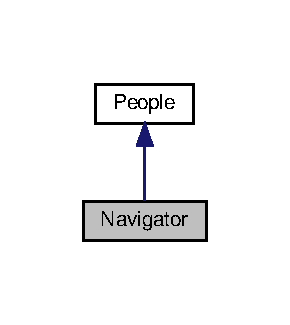
\includegraphics[width=139pt]{classNavigator__inherit__graph}
\end{center}
\end{figure}


Collaboration diagram for Navigator\+:\nopagebreak
\begin{figure}[H]
\begin{center}
\leavevmode
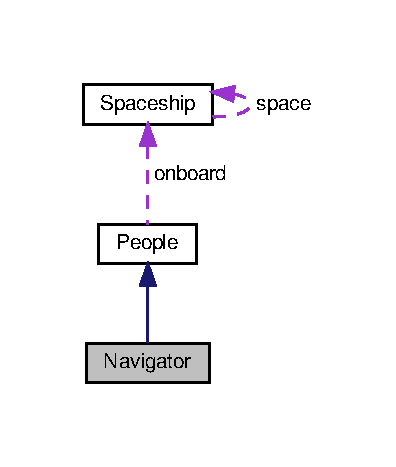
\includegraphics[width=190pt]{classNavigator__coll__graph}
\end{center}
\end{figure}
\subsection*{Public Member Functions}
\begin{DoxyCompactItemize}
\item 
\hyperlink{classNavigator_a59230ab4698882f754d5ce275a1a4030}{Navigator} ()
\item 
\hyperlink{classNavigator_a81bb9c10588736497700032d8b61e9d1}{$\sim$\+Navigator} ()
\item 
void \hyperlink{classNavigator_a7dc06965001f658cff3c5f0dcac39def}{recieve\+Spaceship\+Error} (string)
\item 
void \hyperlink{classNavigator_a72ce12655f579879aae63b118c906b91}{send\+Error\+Message} (string)
\item 
string \hyperlink{classNavigator_a3b6314e429bc38e2cd330db7c187a7ae}{get\+Type} ()
\end{DoxyCompactItemize}
\subsection*{Additional Inherited Members}


\subsection{Detailed Description}
\hyperlink{classNavigator}{Navigator} class. 

\subsection{Constructor \& Destructor Documentation}
\mbox{\Hypertarget{classNavigator_a59230ab4698882f754d5ce275a1a4030}\label{classNavigator_a59230ab4698882f754d5ce275a1a4030}} 
\index{Navigator@{Navigator}!Navigator@{Navigator}}
\index{Navigator@{Navigator}!Navigator@{Navigator}}
\subsubsection{\texorpdfstring{Navigator()}{Navigator()}}
{\footnotesize\ttfamily Navigator\+::\+Navigator (\begin{DoxyParamCaption}{ }\end{DoxyParamCaption})\hspace{0.3cm}{\ttfamily [inline]}}

Default constructor \mbox{\Hypertarget{classNavigator_a81bb9c10588736497700032d8b61e9d1}\label{classNavigator_a81bb9c10588736497700032d8b61e9d1}} 
\index{Navigator@{Navigator}!````~Navigator@{$\sim$\+Navigator}}
\index{````~Navigator@{$\sim$\+Navigator}!Navigator@{Navigator}}
\subsubsection{\texorpdfstring{$\sim$\+Navigator()}{~Navigator()}}
{\footnotesize\ttfamily Navigator\+::$\sim$\+Navigator (\begin{DoxyParamCaption}{ }\end{DoxyParamCaption})\hspace{0.3cm}{\ttfamily [inline]}}

Default desctructor 

\subsection{Member Function Documentation}
\mbox{\Hypertarget{classNavigator_a3b6314e429bc38e2cd330db7c187a7ae}\label{classNavigator_a3b6314e429bc38e2cd330db7c187a7ae}} 
\index{Navigator@{Navigator}!get\+Type@{get\+Type}}
\index{get\+Type@{get\+Type}!Navigator@{Navigator}}
\subsubsection{\texorpdfstring{get\+Type()}{getType()}}
{\footnotesize\ttfamily string Navigator\+::get\+Type (\begin{DoxyParamCaption}{ }\end{DoxyParamCaption})\hspace{0.3cm}{\ttfamily [inline]}, {\ttfamily [virtual]}}

get type of person 

Implements \hyperlink{classPeople_af60dd882d60cddf63f9b95815ce551a8}{People}.

\mbox{\Hypertarget{classNavigator_a7dc06965001f658cff3c5f0dcac39def}\label{classNavigator_a7dc06965001f658cff3c5f0dcac39def}} 
\index{Navigator@{Navigator}!recieve\+Spaceship\+Error@{recieve\+Spaceship\+Error}}
\index{recieve\+Spaceship\+Error@{recieve\+Spaceship\+Error}!Navigator@{Navigator}}
\subsubsection{\texorpdfstring{recieve\+Spaceship\+Error()}{recieveSpaceshipError()}}
{\footnotesize\ttfamily void Navigator\+::recieve\+Spaceship\+Error (\begin{DoxyParamCaption}\item[{string}]{message }\end{DoxyParamCaption})\hspace{0.3cm}{\ttfamily [virtual]}}

Recieve an error from the spaceship 
\begin{DoxyParams}{Parameters}
{\em message} & -\/ the error being received \\
\hline
\end{DoxyParams}


Implements \hyperlink{classPeople_a0685df78be631783138865e03cc7c85d}{People}.

\mbox{\Hypertarget{classNavigator_a72ce12655f579879aae63b118c906b91}\label{classNavigator_a72ce12655f579879aae63b118c906b91}} 
\index{Navigator@{Navigator}!send\+Error\+Message@{send\+Error\+Message}}
\index{send\+Error\+Message@{send\+Error\+Message}!Navigator@{Navigator}}
\subsubsection{\texorpdfstring{send\+Error\+Message()}{sendErrorMessage()}}
{\footnotesize\ttfamily void Navigator\+::send\+Error\+Message (\begin{DoxyParamCaption}\item[{string}]{message }\end{DoxyParamCaption})\hspace{0.3cm}{\ttfamily [virtual]}}

Send an error to the spaceship 
\begin{DoxyParams}{Parameters}
{\em message} & -\/ the error being sent \\
\hline
\end{DoxyParams}


Implements \hyperlink{classPeople_a572a35170f61d1848eb04b65baafb057}{People}.



The documentation for this class was generated from the following files\+:\begin{DoxyCompactItemize}
\item 
Navigator.\+h\item 
Navigator.\+cpp\end{DoxyCompactItemize}

\hypertarget{classNavigatorFactory}{}\section{Navigator\+Factory Class Reference}
\label{classNavigatorFactory}\index{Navigator\+Factory@{Navigator\+Factory}}


\hyperlink{classNavigator}{Navigator} factory class.  




{\ttfamily \#include $<$Navigator\+Factory.\+h$>$}



Inheritance diagram for Navigator\+Factory\+:\nopagebreak
\begin{figure}[H]
\begin{center}
\leavevmode
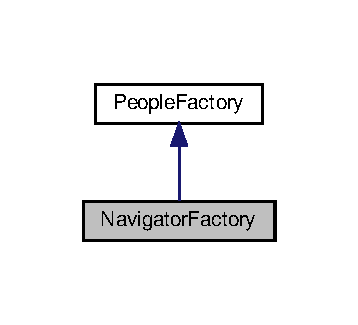
\includegraphics[width=172pt]{classNavigatorFactory__inherit__graph}
\end{center}
\end{figure}


Collaboration diagram for Navigator\+Factory\+:\nopagebreak
\begin{figure}[H]
\begin{center}
\leavevmode
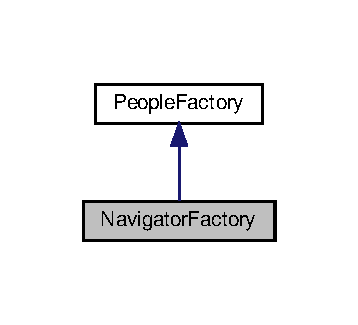
\includegraphics[width=172pt]{classNavigatorFactory__coll__graph}
\end{center}
\end{figure}
\subsection*{Public Member Functions}
\begin{DoxyCompactItemize}
\item 
\hyperlink{classNavigatorFactory_a6dffc936447428b43de6432c3684f43e}{Navigator\+Factory} ()
\item 
\hyperlink{classNavigatorFactory_a761b19635335f0d772196005e443ebd3}{$\sim$\+Navigator\+Factory} ()
\item 
\mbox{\Hypertarget{classNavigatorFactory_ae4db06a5f2ee294e6e540b8922d55313}\label{classNavigatorFactory_ae4db06a5f2ee294e6e540b8922d55313}} 
\hyperlink{classPeople}{People} $\ast$ {\bfseries create} ()
\end{DoxyCompactItemize}


\subsection{Detailed Description}
\hyperlink{classNavigator}{Navigator} factory class. 

\subsection{Constructor \& Destructor Documentation}
\mbox{\Hypertarget{classNavigatorFactory_a6dffc936447428b43de6432c3684f43e}\label{classNavigatorFactory_a6dffc936447428b43de6432c3684f43e}} 
\index{Navigator\+Factory@{Navigator\+Factory}!Navigator\+Factory@{Navigator\+Factory}}
\index{Navigator\+Factory@{Navigator\+Factory}!Navigator\+Factory@{Navigator\+Factory}}
\subsubsection{\texorpdfstring{Navigator\+Factory()}{NavigatorFactory()}}
{\footnotesize\ttfamily Navigator\+Factory\+::\+Navigator\+Factory (\begin{DoxyParamCaption}{ }\end{DoxyParamCaption})\hspace{0.3cm}{\ttfamily [inline]}}

Default constructor \mbox{\Hypertarget{classNavigatorFactory_a761b19635335f0d772196005e443ebd3}\label{classNavigatorFactory_a761b19635335f0d772196005e443ebd3}} 
\index{Navigator\+Factory@{Navigator\+Factory}!````~Navigator\+Factory@{$\sim$\+Navigator\+Factory}}
\index{````~Navigator\+Factory@{$\sim$\+Navigator\+Factory}!Navigator\+Factory@{Navigator\+Factory}}
\subsubsection{\texorpdfstring{$\sim$\+Navigator\+Factory()}{~NavigatorFactory()}}
{\footnotesize\ttfamily Navigator\+Factory\+::$\sim$\+Navigator\+Factory (\begin{DoxyParamCaption}{ }\end{DoxyParamCaption})\hspace{0.3cm}{\ttfamily [inline]}}

Default desctructor 

The documentation for this class was generated from the following file\+:\begin{DoxyCompactItemize}
\item 
Navigator\+Factory.\+h\end{DoxyCompactItemize}

\hypertarget{classNode}{}\section{Node Class Reference}
\label{classNode}\index{Node@{Node}}


Collaboration diagram for Node\+:\nopagebreak
\begin{figure}[H]
\begin{center}
\leavevmode
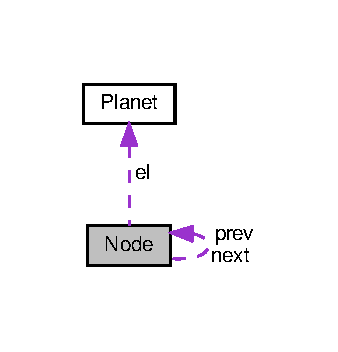
\includegraphics[width=162pt]{classNode__coll__graph}
\end{center}
\end{figure}
\subsection*{Public Attributes}
\begin{DoxyCompactItemize}
\item 
\mbox{\Hypertarget{classNode_a51f48c998114cf08deebf34302472302}\label{classNode_a51f48c998114cf08deebf34302472302}} 
\hyperlink{classPlanet}{Planet} $\ast$ {\bfseries el}
\item 
\mbox{\Hypertarget{classNode_a2559a716f69ccaa76d648d9f1b83065e}\label{classNode_a2559a716f69ccaa76d648d9f1b83065e}} 
\hyperlink{classNode}{Node} $\ast$ {\bfseries next}
\item 
\mbox{\Hypertarget{classNode_a632ea91c6a13082308f7692649a68880}\label{classNode_a632ea91c6a13082308f7692649a68880}} 
\hyperlink{classNode}{Node} $\ast$ {\bfseries prev}
\end{DoxyCompactItemize}


The documentation for this class was generated from the following file\+:\begin{DoxyCompactItemize}
\item 
Node.\+h\end{DoxyCompactItemize}

\hypertarget{classPeople}{}\section{People Class Reference}
\label{classPeople}\index{People@{People}}


\hyperlink{classPeople}{People} class.  




{\ttfamily \#include $<$People.\+h$>$}



Inheritance diagram for People\+:
% FIG 0


Collaboration diagram for People\+:
% FIG 1
\subsection*{Public Member Functions}
\begin{DoxyCompactItemize}
\item 
\hyperlink{classPeople_aae1408eddfd15a5007003ecdf1507941}{People} ()
\item 
virtual \hyperlink{classPeople_a26b0c041fafa38a1f84e0d51742e886a}{$\sim$\+People} ()
\item 
virtual void \hyperlink{classPeople_a0685df78be631783138865e03cc7c85d}{recieve\+Spaceship\+Error} (string)=0
\item 
virtual void \hyperlink{classPeople_a572a35170f61d1848eb04b65baafb057}{send\+Error\+Message} (string)=0
\item 
void \hyperlink{classPeople_a66c99da939fe89614360953a3619a271}{board\+Ship} (\hyperlink{classSpaceship}{Spaceship} $\ast$)
\item 
void \hyperlink{classPeople_a5e87ed1cfd4d4d90b95e3b2196c7687e}{leave\+Ship} ()
\end{DoxyCompactItemize}
\subsection*{Protected Attributes}
\begin{DoxyCompactItemize}
\item 
int \hyperlink{classPeople_ab8216a756c93da727d2626dfb063f82a}{id}
\item 
\hyperlink{classSpaceship}{Spaceship} $\ast$ \hyperlink{classPeople_a103de9b80f0b47e01dc24ac48ec301b2}{onboard}
\end{DoxyCompactItemize}


\subsection{Detailed Description}
\hyperlink{classPeople}{People} class. 

\subsection{Constructor \& Destructor Documentation}
\mbox{\Hypertarget{classPeople_aae1408eddfd15a5007003ecdf1507941}\label{classPeople_aae1408eddfd15a5007003ecdf1507941}} 
\index{People@{People}!People@{People}}
\index{People@{People}!People@{People}}
\subsubsection{\texorpdfstring{People()}{People()}}
{\footnotesize\ttfamily People\+::\+People (\begin{DoxyParamCaption}{ }\end{DoxyParamCaption})\hspace{0.3cm}{\ttfamily [inline]}}

Default constructor \mbox{\Hypertarget{classPeople_a26b0c041fafa38a1f84e0d51742e886a}\label{classPeople_a26b0c041fafa38a1f84e0d51742e886a}} 
\index{People@{People}!````~People@{$\sim$\+People}}
\index{````~People@{$\sim$\+People}!People@{People}}
\subsubsection{\texorpdfstring{$\sim$\+People()}{~People()}}
{\footnotesize\ttfamily virtual People\+::$\sim$\+People (\begin{DoxyParamCaption}{ }\end{DoxyParamCaption})\hspace{0.3cm}{\ttfamily [inline]}, {\ttfamily [virtual]}}

Virtual default desctructor 

\subsection{Member Function Documentation}
\mbox{\Hypertarget{classPeople_a66c99da939fe89614360953a3619a271}\label{classPeople_a66c99da939fe89614360953a3619a271}} 
\index{People@{People}!board\+Ship@{board\+Ship}}
\index{board\+Ship@{board\+Ship}!People@{People}}
\subsubsection{\texorpdfstring{board\+Ship()}{boardShip()}}
{\footnotesize\ttfamily void People\+::board\+Ship (\begin{DoxyParamCaption}\item[{\hyperlink{classSpaceship}{Spaceship} $\ast$}]{s }\end{DoxyParamCaption})}

Board ship. Register with spaceship 
\begin{DoxyParams}{Parameters}
{\em spaceship} & -\/ spaceship being registered \\
\hline
\end{DoxyParams}
\mbox{\Hypertarget{classPeople_a5e87ed1cfd4d4d90b95e3b2196c7687e}\label{classPeople_a5e87ed1cfd4d4d90b95e3b2196c7687e}} 
\index{People@{People}!leave\+Ship@{leave\+Ship}}
\index{leave\+Ship@{leave\+Ship}!People@{People}}
\subsubsection{\texorpdfstring{leave\+Ship()}{leaveShip()}}
{\footnotesize\ttfamily void People\+::leave\+Ship (\begin{DoxyParamCaption}{ }\end{DoxyParamCaption})}

Leave ship. Deregister with spaceship \mbox{\Hypertarget{classPeople_a0685df78be631783138865e03cc7c85d}\label{classPeople_a0685df78be631783138865e03cc7c85d}} 
\index{People@{People}!recieve\+Spaceship\+Error@{recieve\+Spaceship\+Error}}
\index{recieve\+Spaceship\+Error@{recieve\+Spaceship\+Error}!People@{People}}
\subsubsection{\texorpdfstring{recieve\+Spaceship\+Error()}{recieveSpaceshipError()}}
{\footnotesize\ttfamily virtual void People\+::recieve\+Spaceship\+Error (\begin{DoxyParamCaption}\item[{string}]{ }\end{DoxyParamCaption})\hspace{0.3cm}{\ttfamily [pure virtual]}}

Pure virtual recieve error method 
\begin{DoxyParams}{Parameters}
{\em message} & -\/ message being recieved \\
\hline
\end{DoxyParams}


Implemented in \hyperlink{classCommanderOfTheFleet_a13e91b9342df067b375f7ef2b929c0d5}{Commander\+Of\+The\+Fleet}, \hyperlink{classEngineer_acc86ce6b4b1388be8ebacc685f9e6233}{Engineer}, \hyperlink{classComms_a1aed1c01a813afd55309fdc59d2871bf}{Comms}, \hyperlink{classDoctor_a820dca3b9f05d3f69c47bd7318923b88}{Doctor}, \hyperlink{classFighter_aecd2761c68aed8499e210fd0ca11c447}{Fighter}, \hyperlink{classCaptain_a39ebd40ec094b410f295188bb6262009}{Captain}, \hyperlink{classNavigator_a7dc06965001f658cff3c5f0dcac39def}{Navigator}, and \hyperlink{classChiefEngineer_a7170ae93d7eadc1a68bc86c25a9be0db}{Chief\+Engineer}.

\mbox{\Hypertarget{classPeople_a572a35170f61d1848eb04b65baafb057}\label{classPeople_a572a35170f61d1848eb04b65baafb057}} 
\index{People@{People}!send\+Error\+Message@{send\+Error\+Message}}
\index{send\+Error\+Message@{send\+Error\+Message}!People@{People}}
\subsubsection{\texorpdfstring{send\+Error\+Message()}{sendErrorMessage()}}
{\footnotesize\ttfamily virtual void People\+::send\+Error\+Message (\begin{DoxyParamCaption}\item[{string}]{ }\end{DoxyParamCaption})\hspace{0.3cm}{\ttfamily [pure virtual]}}

Pure virtual send error message 
\begin{DoxyParams}{Parameters}
{\em message} & -\/ message being sent \\
\hline
\end{DoxyParams}


Implemented in \hyperlink{classCommanderOfTheFleet_a39cfd5c0016355543515e919791d7984}{Commander\+Of\+The\+Fleet}, \hyperlink{classEngineer_ae60806f33b7f226891dbb7ad9b8a0c0b}{Engineer}, \hyperlink{classComms_a23c37f6d10f06c7cfe25c4dc7d62fa12}{Comms}, \hyperlink{classDoctor_a5a524981ce52102f975cf9c569137ce5}{Doctor}, \hyperlink{classFighter_a42b60e52427e5c69daf141351655805c}{Fighter}, \hyperlink{classCaptain_a88abc1940bcdef8a655efc20ebd68d50}{Captain}, \hyperlink{classNavigator_a72ce12655f579879aae63b118c906b91}{Navigator}, and \hyperlink{classChiefEngineer_afe5a4677f7651fff2926c0583875a666}{Chief\+Engineer}.



\subsection{Member Data Documentation}
\mbox{\Hypertarget{classPeople_ab8216a756c93da727d2626dfb063f82a}\label{classPeople_ab8216a756c93da727d2626dfb063f82a}} 
\index{People@{People}!id@{id}}
\index{id@{id}!People@{People}}
\subsubsection{\texorpdfstring{id}{id}}
{\footnotesize\ttfamily int People\+::id\hspace{0.3cm}{\ttfamily [protected]}}

ID variable used for uniquely identifying which person is being registered with the Mediator(\+Spaceship) \mbox{\Hypertarget{classPeople_a103de9b80f0b47e01dc24ac48ec301b2}\label{classPeople_a103de9b80f0b47e01dc24ac48ec301b2}} 
\index{People@{People}!onboard@{onboard}}
\index{onboard@{onboard}!People@{People}}
\subsubsection{\texorpdfstring{onboard}{onboard}}
{\footnotesize\ttfamily \hyperlink{classSpaceship}{Spaceship}$\ast$ People\+::onboard\hspace{0.3cm}{\ttfamily [protected]}}

Which spaceship this person is onboard 

The documentation for this class was generated from the following files\+:\begin{DoxyCompactItemize}
\item 
People.\+h\item 
People.\+cpp\end{DoxyCompactItemize}

\hypertarget{classPeopleFactory}{}\section{People\+Factory Class Reference}
\label{classPeopleFactory}\index{People\+Factory@{People\+Factory}}


\hyperlink{classPeople}{People} Factory class.  




{\ttfamily \#include $<$People\+Factory.\+h$>$}



Inheritance diagram for People\+Factory\+:\nopagebreak
\begin{figure}[H]
\begin{center}
\leavevmode
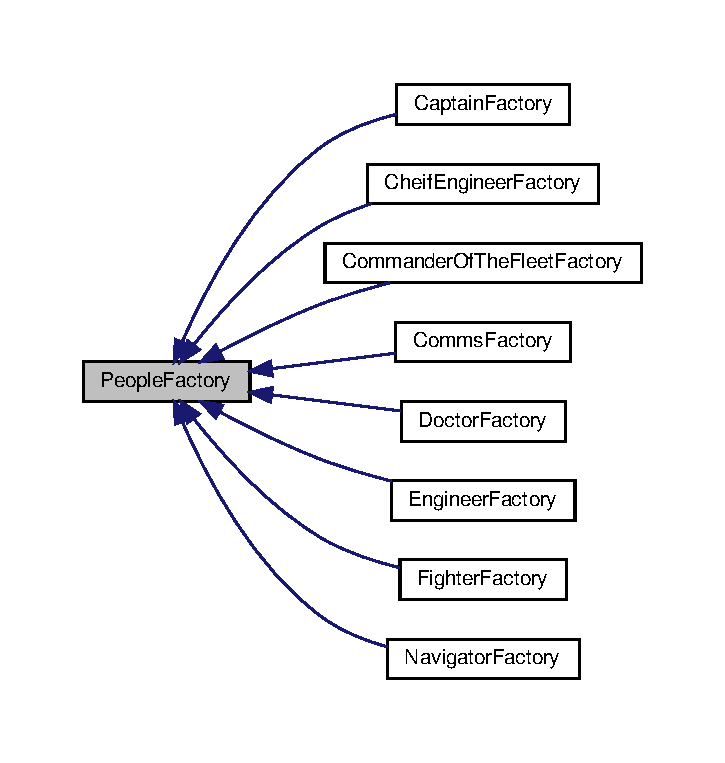
\includegraphics[width=348pt]{classPeopleFactory__inherit__graph}
\end{center}
\end{figure}
\subsection*{Public Member Functions}
\begin{DoxyCompactItemize}
\item 
\hyperlink{classPeopleFactory_a937ce020364a355d6689c365ba70f0d6}{People\+Factory} ()
\item 
\hyperlink{classPeopleFactory_a18d1aec526ba93ca84cde1c25cfb8944}{$\sim$\+People\+Factory} ()
\item 
\mbox{\Hypertarget{classPeopleFactory_a2a61d6ec85c72d8b1c28752609e60d10}\label{classPeopleFactory_a2a61d6ec85c72d8b1c28752609e60d10}} 
virtual \hyperlink{classPeople}{People} $\ast$ {\bfseries create} ()=0
\end{DoxyCompactItemize}


\subsection{Detailed Description}
\hyperlink{classPeople}{People} Factory class. 

\subsection{Constructor \& Destructor Documentation}
\mbox{\Hypertarget{classPeopleFactory_a937ce020364a355d6689c365ba70f0d6}\label{classPeopleFactory_a937ce020364a355d6689c365ba70f0d6}} 
\index{People\+Factory@{People\+Factory}!People\+Factory@{People\+Factory}}
\index{People\+Factory@{People\+Factory}!People\+Factory@{People\+Factory}}
\subsubsection{\texorpdfstring{People\+Factory()}{PeopleFactory()}}
{\footnotesize\ttfamily People\+Factory\+::\+People\+Factory (\begin{DoxyParamCaption}{ }\end{DoxyParamCaption})\hspace{0.3cm}{\ttfamily [inline]}}

Default constructor \mbox{\Hypertarget{classPeopleFactory_a18d1aec526ba93ca84cde1c25cfb8944}\label{classPeopleFactory_a18d1aec526ba93ca84cde1c25cfb8944}} 
\index{People\+Factory@{People\+Factory}!````~People\+Factory@{$\sim$\+People\+Factory}}
\index{````~People\+Factory@{$\sim$\+People\+Factory}!People\+Factory@{People\+Factory}}
\subsubsection{\texorpdfstring{$\sim$\+People\+Factory()}{~PeopleFactory()}}
{\footnotesize\ttfamily People\+Factory\+::$\sim$\+People\+Factory (\begin{DoxyParamCaption}{ }\end{DoxyParamCaption})\hspace{0.3cm}{\ttfamily [inline]}}

Default desctructor 

The documentation for this class was generated from the following file\+:\begin{DoxyCompactItemize}
\item 
People\+Factory.\+h\end{DoxyCompactItemize}

\hypertarget{classPeopleMediatior}{}\section{People\+Mediatior Class Reference}
\label{classPeopleMediatior}\index{People\+Mediatior@{People\+Mediatior}}


The documentation for this class was generated from the following file\+:\begin{DoxyCompactItemize}
\item 
\hyperlink{PeopleMediator_8h}{People\+Mediator.\+h}\end{DoxyCompactItemize}

\hypertarget{classPlanet}{}\section{Planet Class Reference}
\label{classPlanet}\index{Planet@{Planet}}


\hyperlink{classPlanet}{Planet} class.  




{\ttfamily \#include $<$Planet.\+h$>$}

\subsection*{Public Member Functions}
\begin{DoxyCompactItemize}
\item 
\hyperlink{classPlanet_ae98ce54858c1174201987d73228fa29b}{Planet} (string n)
\item 
\hyperlink{classPlanet_afd66d974488511c495e6e5aa2e886085}{Planet} (string n, double rR, double tL)
\item 
\hyperlink{classPlanet_aaa1aaed9d4ef90b4836531edb7b18e0a}{$\sim$\+Planet} ()
\item 
\mbox{\Hypertarget{classPlanet_ab8b1c3018f15bb37af41371526c6bbe2}\label{classPlanet_ab8b1c3018f15bb37af41371526c6bbe2}} 
double {\bfseries get\+Resource\+Rate} ()
\item 
\mbox{\Hypertarget{classPlanet_a4bda8bf9239f4d3c7a0a60a1ed52edea}\label{classPlanet_a4bda8bf9239f4d3c7a0a60a1ed52edea}} 
double {\bfseries get\+Threat\+Level} ()
\item 
\mbox{\Hypertarget{classPlanet_a305bd81b25e55ad28cb966b5ac4e4dce}\label{classPlanet_a305bd81b25e55ad28cb966b5ac4e4dce}} 
void {\bfseries set\+Resource\+Rate} (double)
\item 
\mbox{\Hypertarget{classPlanet_a765f62442f84f54666f9975633478930}\label{classPlanet_a765f62442f84f54666f9975633478930}} 
void {\bfseries set\+Threat\+Level} (double)
\item 
\mbox{\Hypertarget{classPlanet_aea9b459b5f5d28555632a1e334cd8d3a}\label{classPlanet_aea9b459b5f5d28555632a1e334cd8d3a}} 
void {\bfseries accept} (\hyperlink{classSpaceship}{Spaceship} $\ast$s)
\end{DoxyCompactItemize}


\subsection{Detailed Description}
\hyperlink{classPlanet}{Planet} class. 

\subsection{Constructor \& Destructor Documentation}
\mbox{\Hypertarget{classPlanet_ae98ce54858c1174201987d73228fa29b}\label{classPlanet_ae98ce54858c1174201987d73228fa29b}} 
\index{Planet@{Planet}!Planet@{Planet}}
\index{Planet@{Planet}!Planet@{Planet}}
\subsubsection{\texorpdfstring{Planet()}{Planet()}\hspace{0.1cm}{\footnotesize\ttfamily [1/2]}}
{\footnotesize\ttfamily Planet\+::\+Planet (\begin{DoxyParamCaption}\item[{string}]{n }\end{DoxyParamCaption})}

default constructor \mbox{\Hypertarget{classPlanet_afd66d974488511c495e6e5aa2e886085}\label{classPlanet_afd66d974488511c495e6e5aa2e886085}} 
\index{Planet@{Planet}!Planet@{Planet}}
\index{Planet@{Planet}!Planet@{Planet}}
\subsubsection{\texorpdfstring{Planet()}{Planet()}\hspace{0.1cm}{\footnotesize\ttfamily [2/2]}}
{\footnotesize\ttfamily Planet\+::\+Planet (\begin{DoxyParamCaption}\item[{string}]{n,  }\item[{double}]{rR,  }\item[{double}]{tL }\end{DoxyParamCaption})}

Paramaterised constructor \mbox{\Hypertarget{classPlanet_aaa1aaed9d4ef90b4836531edb7b18e0a}\label{classPlanet_aaa1aaed9d4ef90b4836531edb7b18e0a}} 
\index{Planet@{Planet}!````~Planet@{$\sim$\+Planet}}
\index{````~Planet@{$\sim$\+Planet}!Planet@{Planet}}
\subsubsection{\texorpdfstring{$\sim$\+Planet()}{~Planet()}}
{\footnotesize\ttfamily Planet\+::$\sim$\+Planet (\begin{DoxyParamCaption}{ }\end{DoxyParamCaption})}

Default Destructor 

The documentation for this class was generated from the following files\+:\begin{DoxyCompactItemize}
\item 
Planet.\+h\item 
Planet.\+cpp\end{DoxyCompactItemize}

\hypertarget{classPlanetIterator}{}\section{Planet\+Iterator Class Reference}
\label{classPlanetIterator}\index{Planet\+Iterator@{Planet\+Iterator}}


\hyperlink{classPlanet}{Planet} Iterator class.  




{\ttfamily \#include $<$Planet\+Iterator.\+h$>$}



Collaboration diagram for Planet\+Iterator\+:\nopagebreak
\begin{figure}[H]
\begin{center}
\leavevmode
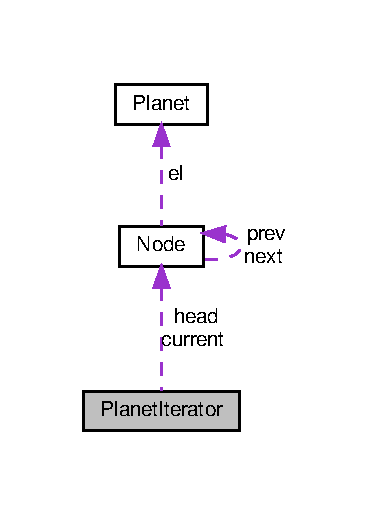
\includegraphics[width=178pt]{classPlanetIterator__coll__graph}
\end{center}
\end{figure}
\subsection*{Public Member Functions}
\begin{DoxyCompactItemize}
\item 
\hyperlink{classPlanetIterator_ac0769a13686b355e55e687de11231d9c}{Planet\+Iterator} ()
\item 
\hyperlink{classPlanet}{Planet} \& \hyperlink{classPlanetIterator_a71bfc8a3a3eec78ab1a1f6cc2a7a1cf8}{operator$\ast$} ()
\item 
\hyperlink{classPlanetIterator}{Planet\+Iterator} \hyperlink{classPlanetIterator_a8e057fb430e49f56f756c070e95587b3}{operator++} ()
\item 
bool \hyperlink{classPlanetIterator_a8c8b0f27933c69f40efd523815acce3a}{operator==} (const \hyperlink{classPlanetIterator}{Planet\+Iterator} \&) const
\end{DoxyCompactItemize}
\subsection*{Protected Member Functions}
\begin{DoxyCompactItemize}
\item 
\hyperlink{classPlanetIterator_ab5c84527dd5b82051e9f59c650dbd5bc}{Planet\+Iterator} (const \hyperlink{classPlanetQueue}{Planet\+Queue} \&, \hyperlink{classNode}{Node} $\ast$)
\end{DoxyCompactItemize}
\subsection*{Protected Attributes}
\begin{DoxyCompactItemize}
\item 
\mbox{\Hypertarget{classPlanetIterator_a8b284f4aa03057d485c42d1962ab9939}\label{classPlanetIterator_a8b284f4aa03057d485c42d1962ab9939}} 
\hyperlink{classNode}{Node} $\ast$ {\bfseries head}
\item 
\mbox{\Hypertarget{classPlanetIterator_a00c46ae901520be5ff52c38eaa08a3b6}\label{classPlanetIterator_a00c46ae901520be5ff52c38eaa08a3b6}} 
\hyperlink{classNode}{Node} $\ast$ {\bfseries current}
\end{DoxyCompactItemize}
\subsection*{Friends}
\begin{DoxyCompactItemize}
\item 
\mbox{\Hypertarget{classPlanetIterator_af4641bececf1b32ed2e8b02c382d7e77}\label{classPlanetIterator_af4641bececf1b32ed2e8b02c382d7e77}} 
class {\bfseries Planet\+Queue}
\end{DoxyCompactItemize}


\subsection{Detailed Description}
\hyperlink{classPlanet}{Planet} Iterator class. 

\subsection{Constructor \& Destructor Documentation}
\mbox{\Hypertarget{classPlanetIterator_ac0769a13686b355e55e687de11231d9c}\label{classPlanetIterator_ac0769a13686b355e55e687de11231d9c}} 
\index{Planet\+Iterator@{Planet\+Iterator}!Planet\+Iterator@{Planet\+Iterator}}
\index{Planet\+Iterator@{Planet\+Iterator}!Planet\+Iterator@{Planet\+Iterator}}
\subsubsection{\texorpdfstring{Planet\+Iterator()}{PlanetIterator()}\hspace{0.1cm}{\footnotesize\ttfamily [1/2]}}
{\footnotesize\ttfamily Planet\+Iterator\+::\+Planet\+Iterator (\begin{DoxyParamCaption}{ }\end{DoxyParamCaption})}

default constructor \mbox{\Hypertarget{classPlanetIterator_ab5c84527dd5b82051e9f59c650dbd5bc}\label{classPlanetIterator_ab5c84527dd5b82051e9f59c650dbd5bc}} 
\index{Planet\+Iterator@{Planet\+Iterator}!Planet\+Iterator@{Planet\+Iterator}}
\index{Planet\+Iterator@{Planet\+Iterator}!Planet\+Iterator@{Planet\+Iterator}}
\subsubsection{\texorpdfstring{Planet\+Iterator()}{PlanetIterator()}\hspace{0.1cm}{\footnotesize\ttfamily [2/2]}}
{\footnotesize\ttfamily Planet\+Iterator\+::\+Planet\+Iterator (\begin{DoxyParamCaption}\item[{const \hyperlink{classPlanetQueue}{Planet\+Queue} \&}]{source,  }\item[{\hyperlink{classNode}{Node} $\ast$}]{p }\end{DoxyParamCaption})\hspace{0.3cm}{\ttfamily [protected]}}

Paramaterised constructor 

\subsection{Member Function Documentation}
\mbox{\Hypertarget{classPlanetIterator_a71bfc8a3a3eec78ab1a1f6cc2a7a1cf8}\label{classPlanetIterator_a71bfc8a3a3eec78ab1a1f6cc2a7a1cf8}} 
\index{Planet\+Iterator@{Planet\+Iterator}!operator$\ast$@{operator$\ast$}}
\index{operator$\ast$@{operator$\ast$}!Planet\+Iterator@{Planet\+Iterator}}
\subsubsection{\texorpdfstring{operator$\ast$()}{operator*()}}
{\footnotesize\ttfamily \hyperlink{classPlanet}{Planet}\& Planet\+Iterator\+::operator$\ast$ (\begin{DoxyParamCaption}{ }\end{DoxyParamCaption})}

Overridden $\ast$ operator \mbox{\Hypertarget{classPlanetIterator_a8e057fb430e49f56f756c070e95587b3}\label{classPlanetIterator_a8e057fb430e49f56f756c070e95587b3}} 
\index{Planet\+Iterator@{Planet\+Iterator}!operator++@{operator++}}
\index{operator++@{operator++}!Planet\+Iterator@{Planet\+Iterator}}
\subsubsection{\texorpdfstring{operator++()}{operator++()}}
{\footnotesize\ttfamily \hyperlink{classPlanetIterator}{Planet\+Iterator} Planet\+Iterator\+::operator++ (\begin{DoxyParamCaption}{ }\end{DoxyParamCaption})}

Overidden ++ operator \mbox{\Hypertarget{classPlanetIterator_a8c8b0f27933c69f40efd523815acce3a}\label{classPlanetIterator_a8c8b0f27933c69f40efd523815acce3a}} 
\index{Planet\+Iterator@{Planet\+Iterator}!operator==@{operator==}}
\index{operator==@{operator==}!Planet\+Iterator@{Planet\+Iterator}}
\subsubsection{\texorpdfstring{operator==()}{operator==()}}
{\footnotesize\ttfamily bool Planet\+Iterator\+::operator== (\begin{DoxyParamCaption}\item[{const \hyperlink{classPlanetIterator}{Planet\+Iterator} \&}]{rhs }\end{DoxyParamCaption}) const}

Overidden == operator 

The documentation for this class was generated from the following files\+:\begin{DoxyCompactItemize}
\item 
Planet\+Iterator.\+h\item 
Planet\+Iterator.\+cpp\end{DoxyCompactItemize}

\hypertarget{classPlanetQueue}{}\section{Planet\+Queue Class Reference}
\label{classPlanetQueue}\index{Planet\+Queue@{Planet\+Queue}}


\hyperlink{classPlanetQueue}{Planet\+Queue} class.  




{\ttfamily \#include $<$Planet\+Queue.\+h$>$}

\subsection*{Public Member Functions}
\begin{DoxyCompactItemize}
\item 
\hyperlink{classPlanetQueue_aece3bd14bfbffdd61c5413bac9d92abf}{Planet\+Queue} ()
\item 
\hyperlink{classPlanetQueue_a401c7ec48201e2a9941ca9c952491f52}{$\sim$\+Planet\+Queue} ()
\item 
bool \hyperlink{classPlanetQueue_a50400f0c70785492f23f2703d9eac0cc}{is\+Empty} ()
\item 
\hyperlink{classPlanetIterator}{Planet\+Iterator} \hyperlink{classPlanetQueue_a00290482aee16d320ce429a03437751c}{begin} ()
\item 
\hyperlink{classPlanetIterator}{Planet\+Iterator} \hyperlink{classPlanetQueue_a587798b5e8ce4c647804379abbbcfd26}{end} ()
\item 
void \hyperlink{classPlanetQueue_a6876331ffc6b56a0e960e0be397babbb}{enqueue} (\hyperlink{classPlanet}{Planet} $\ast$p)
\item 
\hyperlink{classPlanet}{Planet} $\ast$ \hyperlink{classPlanetQueue_a9d64880eea8788b78ebb1b2f430f9f1f}{dequeue} ()
\end{DoxyCompactItemize}
\subsection*{Friends}
\begin{DoxyCompactItemize}
\item 
\mbox{\Hypertarget{classPlanetQueue_a58d980e86656218a4f34476255718e53}\label{classPlanetQueue_a58d980e86656218a4f34476255718e53}} 
class {\bfseries Planet\+Iterator}
\end{DoxyCompactItemize}


\subsection{Detailed Description}
\hyperlink{classPlanetQueue}{Planet\+Queue} class. 

\subsection{Constructor \& Destructor Documentation}
\mbox{\Hypertarget{classPlanetQueue_aece3bd14bfbffdd61c5413bac9d92abf}\label{classPlanetQueue_aece3bd14bfbffdd61c5413bac9d92abf}} 
\index{Planet\+Queue@{Planet\+Queue}!Planet\+Queue@{Planet\+Queue}}
\index{Planet\+Queue@{Planet\+Queue}!Planet\+Queue@{Planet\+Queue}}
\subsubsection{\texorpdfstring{Planet\+Queue()}{PlanetQueue()}}
{\footnotesize\ttfamily Planet\+Queue\+::\+Planet\+Queue (\begin{DoxyParamCaption}{ }\end{DoxyParamCaption})}

Default constructor \mbox{\Hypertarget{classPlanetQueue_a401c7ec48201e2a9941ca9c952491f52}\label{classPlanetQueue_a401c7ec48201e2a9941ca9c952491f52}} 
\index{Planet\+Queue@{Planet\+Queue}!````~Planet\+Queue@{$\sim$\+Planet\+Queue}}
\index{````~Planet\+Queue@{$\sim$\+Planet\+Queue}!Planet\+Queue@{Planet\+Queue}}
\subsubsection{\texorpdfstring{$\sim$\+Planet\+Queue()}{~PlanetQueue()}}
{\footnotesize\ttfamily Planet\+Queue\+::$\sim$\+Planet\+Queue (\begin{DoxyParamCaption}{ }\end{DoxyParamCaption})}

default destructor 

\subsection{Member Function Documentation}
\mbox{\Hypertarget{classPlanetQueue_a00290482aee16d320ce429a03437751c}\label{classPlanetQueue_a00290482aee16d320ce429a03437751c}} 
\index{Planet\+Queue@{Planet\+Queue}!begin@{begin}}
\index{begin@{begin}!Planet\+Queue@{Planet\+Queue}}
\subsubsection{\texorpdfstring{begin()}{begin()}}
{\footnotesize\ttfamily \hyperlink{classPlanetIterator}{Planet\+Iterator} Planet\+Queue\+::begin (\begin{DoxyParamCaption}{ }\end{DoxyParamCaption})}

Start of the queue \begin{DoxyReturn}{Returns}
\hyperlink{classPlanetIterator}{Planet\+Iterator} 
\end{DoxyReturn}
\mbox{\Hypertarget{classPlanetQueue_a9d64880eea8788b78ebb1b2f430f9f1f}\label{classPlanetQueue_a9d64880eea8788b78ebb1b2f430f9f1f}} 
\index{Planet\+Queue@{Planet\+Queue}!dequeue@{dequeue}}
\index{dequeue@{dequeue}!Planet\+Queue@{Planet\+Queue}}
\subsubsection{\texorpdfstring{dequeue()}{dequeue()}}
{\footnotesize\ttfamily \hyperlink{classPlanet}{Planet} $\ast$ Planet\+Queue\+::dequeue (\begin{DoxyParamCaption}{ }\end{DoxyParamCaption})}

Dequeue a planet \mbox{\Hypertarget{classPlanetQueue_a587798b5e8ce4c647804379abbbcfd26}\label{classPlanetQueue_a587798b5e8ce4c647804379abbbcfd26}} 
\index{Planet\+Queue@{Planet\+Queue}!end@{end}}
\index{end@{end}!Planet\+Queue@{Planet\+Queue}}
\subsubsection{\texorpdfstring{end()}{end()}}
{\footnotesize\ttfamily \hyperlink{classPlanetIterator}{Planet\+Iterator} Planet\+Queue\+::end (\begin{DoxyParamCaption}{ }\end{DoxyParamCaption})}

End of the queue \begin{DoxyReturn}{Returns}
\hyperlink{classPlanetIterator}{Planet\+Iterator} 
\end{DoxyReturn}
\mbox{\Hypertarget{classPlanetQueue_a6876331ffc6b56a0e960e0be397babbb}\label{classPlanetQueue_a6876331ffc6b56a0e960e0be397babbb}} 
\index{Planet\+Queue@{Planet\+Queue}!enqueue@{enqueue}}
\index{enqueue@{enqueue}!Planet\+Queue@{Planet\+Queue}}
\subsubsection{\texorpdfstring{enqueue()}{enqueue()}}
{\footnotesize\ttfamily void Planet\+Queue\+::enqueue (\begin{DoxyParamCaption}\item[{\hyperlink{classPlanet}{Planet} $\ast$}]{p }\end{DoxyParamCaption})}

Enqueue planet into queue 
\begin{DoxyParams}{Parameters}
{\em p} & -\/ \hyperlink{classPlanet}{Planet} to enqueue \\
\hline
\end{DoxyParams}
\mbox{\Hypertarget{classPlanetQueue_a50400f0c70785492f23f2703d9eac0cc}\label{classPlanetQueue_a50400f0c70785492f23f2703d9eac0cc}} 
\index{Planet\+Queue@{Planet\+Queue}!is\+Empty@{is\+Empty}}
\index{is\+Empty@{is\+Empty}!Planet\+Queue@{Planet\+Queue}}
\subsubsection{\texorpdfstring{is\+Empty()}{isEmpty()}}
{\footnotesize\ttfamily bool Planet\+Queue\+::is\+Empty (\begin{DoxyParamCaption}{ }\end{DoxyParamCaption})}

Is the queue empty \begin{DoxyReturn}{Returns}
bool 
\end{DoxyReturn}


The documentation for this class was generated from the following files\+:\begin{DoxyCompactItemize}
\item 
Planet\+Queue.\+h\item 
Planet\+Queue.\+cpp\end{DoxyCompactItemize}

\hypertarget{classRefuelStation}{}\section{Refuel\+Station Class Reference}
\label{classRefuelStation}\index{Refuel\+Station@{Refuel\+Station}}


Refuel station class.  




{\ttfamily \#include $<$Refuel\+Station.\+h$>$}



Inheritance diagram for Refuel\+Station\+:\nopagebreak
\begin{figure}[H]
\begin{center}
\leavevmode
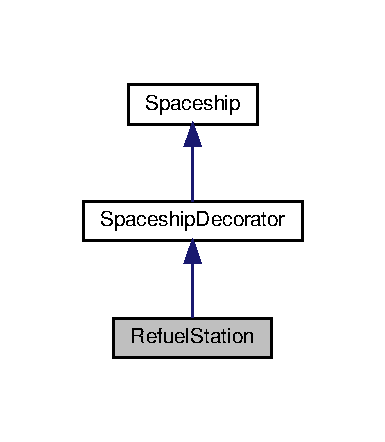
\includegraphics[width=185pt]{classRefuelStation__inherit__graph}
\end{center}
\end{figure}


Collaboration diagram for Refuel\+Station\+:\nopagebreak
\begin{figure}[H]
\begin{center}
\leavevmode
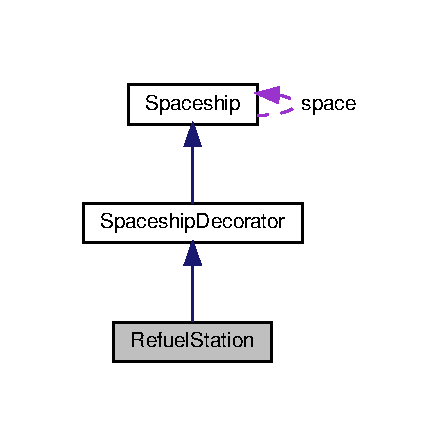
\includegraphics[width=212pt]{classRefuelStation__coll__graph}
\end{center}
\end{figure}
\subsection*{Public Member Functions}
\begin{DoxyCompactItemize}
\item 
\hyperlink{classRefuelStation_a3ab9b746bd1e7bfaa9eff06567d6a1d4}{Refuel\+Station} ()
\item 
\hyperlink{classRefuelStation_afc0ebc020ef08d8a6a2096bdb2f3e314}{$\sim$\+Refuel\+Station} ()
\item 
void \hyperlink{classRefuelStation_a1b14f9c75c883e3288c52a32b2bbd8a4}{refuel\+Spaceship} (\hyperlink{classSpaceship}{Spaceship} $\ast$s)
\item 
void \hyperlink{classRefuelStation_a03510ee8365b5095ca80fac0c5a0a780}{add\+Ship} (\hyperlink{classSpaceship}{Spaceship} $\ast$s)
\item 
double \hyperlink{classRefuelStation_a69c7e7aca14ba70f4d2c4c11e43b4bb4}{get\+Resources} (double a, double b)
\item 
void \hyperlink{classRefuelStation_a6bd40214cf5dc4d46739943f545c6d7a}{add\+Person} (\hyperlink{classPeople}{People} $\ast$p)
\item 
void \hyperlink{classRefuelStation_ae87ea232171fbb09e14b2da82ae3af56}{visit} (\hyperlink{classPlanet}{Planet} $\ast$p)
\item 
\hyperlink{classMemento}{Memento} $\ast$ \hyperlink{classRefuelStation_abd79d981cc7650d6417b8c8166a3fb85}{create\+Memento} (vector$<$ \hyperlink{classSpaceship}{Spaceship} $\ast$$>$ s)
\item 
void \hyperlink{classRefuelStation_aa984ee5ed5a4cea0b96ba1c3903a1b1c}{reinstate\+Memento} (\hyperlink{classMemento}{Memento} $\ast$mem)
\item 
void \hyperlink{classRefuelStation_aa8fccc0887cac98193803762533f9ab1}{execute\+Strategy} ()
\item 
void \hyperlink{classRefuelStation_a1dfda37915eca25344aa2fdeaacab4b4}{select\+Strategy} (\hyperlink{classStrategy}{Strategy} $\ast$s)
\end{DoxyCompactItemize}
\subsection*{Additional Inherited Members}


\subsection{Detailed Description}
Refuel station class. 

\subsection{Constructor \& Destructor Documentation}
\mbox{\Hypertarget{classRefuelStation_a3ab9b746bd1e7bfaa9eff06567d6a1d4}\label{classRefuelStation_a3ab9b746bd1e7bfaa9eff06567d6a1d4}} 
\index{Refuel\+Station@{Refuel\+Station}!Refuel\+Station@{Refuel\+Station}}
\index{Refuel\+Station@{Refuel\+Station}!Refuel\+Station@{Refuel\+Station}}
\subsubsection{\texorpdfstring{Refuel\+Station()}{RefuelStation()}}
{\footnotesize\ttfamily Refuel\+Station\+::\+Refuel\+Station (\begin{DoxyParamCaption}{ }\end{DoxyParamCaption})}

Default constructor \mbox{\Hypertarget{classRefuelStation_afc0ebc020ef08d8a6a2096bdb2f3e314}\label{classRefuelStation_afc0ebc020ef08d8a6a2096bdb2f3e314}} 
\index{Refuel\+Station@{Refuel\+Station}!````~Refuel\+Station@{$\sim$\+Refuel\+Station}}
\index{````~Refuel\+Station@{$\sim$\+Refuel\+Station}!Refuel\+Station@{Refuel\+Station}}
\subsubsection{\texorpdfstring{$\sim$\+Refuel\+Station()}{~RefuelStation()}}
{\footnotesize\ttfamily Refuel\+Station\+::$\sim$\+Refuel\+Station (\begin{DoxyParamCaption}{ }\end{DoxyParamCaption})}

Default desctructor 

\subsection{Member Function Documentation}
\mbox{\Hypertarget{classRefuelStation_a6bd40214cf5dc4d46739943f545c6d7a}\label{classRefuelStation_a6bd40214cf5dc4d46739943f545c6d7a}} 
\index{Refuel\+Station@{Refuel\+Station}!add\+Person@{add\+Person}}
\index{add\+Person@{add\+Person}!Refuel\+Station@{Refuel\+Station}}
\subsubsection{\texorpdfstring{add\+Person()}{addPerson()}}
{\footnotesize\ttfamily void Refuel\+Station\+::add\+Person (\begin{DoxyParamCaption}\item[{\hyperlink{classPeople}{People} $\ast$}]{p }\end{DoxyParamCaption})\hspace{0.3cm}{\ttfamily [inline]}, {\ttfamily [virtual]}}

stub for add\+Person 

Reimplemented from \hyperlink{classSpaceshipDecorator_a6e289d8a65f35b9f223255ae0eaa3b00}{Spaceship\+Decorator}.

\mbox{\Hypertarget{classRefuelStation_a03510ee8365b5095ca80fac0c5a0a780}\label{classRefuelStation_a03510ee8365b5095ca80fac0c5a0a780}} 
\index{Refuel\+Station@{Refuel\+Station}!add\+Ship@{add\+Ship}}
\index{add\+Ship@{add\+Ship}!Refuel\+Station@{Refuel\+Station}}
\subsubsection{\texorpdfstring{add\+Ship()}{addShip()}}
{\footnotesize\ttfamily void Refuel\+Station\+::add\+Ship (\begin{DoxyParamCaption}\item[{\hyperlink{classSpaceship}{Spaceship} $\ast$}]{s }\end{DoxyParamCaption})\hspace{0.3cm}{\ttfamily [inline]}, {\ttfamily [virtual]}}

Virtual add\+Ship 

Reimplemented from \hyperlink{classSpaceshipDecorator_a5ed39419f5fab65dd4af11bf5136f7a4}{Spaceship\+Decorator}.

\mbox{\Hypertarget{classRefuelStation_abd79d981cc7650d6417b8c8166a3fb85}\label{classRefuelStation_abd79d981cc7650d6417b8c8166a3fb85}} 
\index{Refuel\+Station@{Refuel\+Station}!create\+Memento@{create\+Memento}}
\index{create\+Memento@{create\+Memento}!Refuel\+Station@{Refuel\+Station}}
\subsubsection{\texorpdfstring{create\+Memento()}{createMemento()}}
{\footnotesize\ttfamily \hyperlink{classMemento}{Memento}$\ast$ Refuel\+Station\+::create\+Memento (\begin{DoxyParamCaption}\item[{vector$<$ \hyperlink{classSpaceship}{Spaceship} $\ast$$>$}]{s }\end{DoxyParamCaption})\hspace{0.3cm}{\ttfamily [inline]}, {\ttfamily [virtual]}}

create memento stub 

Reimplemented from \hyperlink{classSpaceship_a6d272f846b019dec8226ddab65648a7b}{Spaceship}.

\mbox{\Hypertarget{classRefuelStation_aa8fccc0887cac98193803762533f9ab1}\label{classRefuelStation_aa8fccc0887cac98193803762533f9ab1}} 
\index{Refuel\+Station@{Refuel\+Station}!execute\+Strategy@{execute\+Strategy}}
\index{execute\+Strategy@{execute\+Strategy}!Refuel\+Station@{Refuel\+Station}}
\subsubsection{\texorpdfstring{execute\+Strategy()}{executeStrategy()}}
{\footnotesize\ttfamily void Refuel\+Station\+::execute\+Strategy (\begin{DoxyParamCaption}{ }\end{DoxyParamCaption})\hspace{0.3cm}{\ttfamily [inline]}, {\ttfamily [virtual]}}

execute strategy 

Reimplemented from \hyperlink{classSpaceship}{Spaceship}.

\mbox{\Hypertarget{classRefuelStation_a69c7e7aca14ba70f4d2c4c11e43b4bb4}\label{classRefuelStation_a69c7e7aca14ba70f4d2c4c11e43b4bb4}} 
\index{Refuel\+Station@{Refuel\+Station}!get\+Resources@{get\+Resources}}
\index{get\+Resources@{get\+Resources}!Refuel\+Station@{Refuel\+Station}}
\subsubsection{\texorpdfstring{get\+Resources()}{getResources()}}
{\footnotesize\ttfamily double Refuel\+Station\+::get\+Resources (\begin{DoxyParamCaption}\item[{double}]{a,  }\item[{double}]{b }\end{DoxyParamCaption})\hspace{0.3cm}{\ttfamily [inline]}, {\ttfamily [virtual]}}

stub resource collection 

Reimplemented from \hyperlink{classSpaceshipDecorator_a5ee7a9a8c146c85f08591e47d971dce7}{Spaceship\+Decorator}.

\mbox{\Hypertarget{classRefuelStation_a1b14f9c75c883e3288c52a32b2bbd8a4}\label{classRefuelStation_a1b14f9c75c883e3288c52a32b2bbd8a4}} 
\index{Refuel\+Station@{Refuel\+Station}!refuel\+Spaceship@{refuel\+Spaceship}}
\index{refuel\+Spaceship@{refuel\+Spaceship}!Refuel\+Station@{Refuel\+Station}}
\subsubsection{\texorpdfstring{refuel\+Spaceship()}{refuelSpaceship()}}
{\footnotesize\ttfamily void Refuel\+Station\+::refuel\+Spaceship (\begin{DoxyParamCaption}\item[{\hyperlink{classSpaceship}{Spaceship} $\ast$}]{s }\end{DoxyParamCaption})}

Refuel spaceships that have used all their resources 
\begin{DoxyParams}{Parameters}
{\em s} & -\/ spaceship to be refueled \\
\hline
\end{DoxyParams}
\mbox{\Hypertarget{classRefuelStation_aa984ee5ed5a4cea0b96ba1c3903a1b1c}\label{classRefuelStation_aa984ee5ed5a4cea0b96ba1c3903a1b1c}} 
\index{Refuel\+Station@{Refuel\+Station}!reinstate\+Memento@{reinstate\+Memento}}
\index{reinstate\+Memento@{reinstate\+Memento}!Refuel\+Station@{Refuel\+Station}}
\subsubsection{\texorpdfstring{reinstate\+Memento()}{reinstateMemento()}}
{\footnotesize\ttfamily void Refuel\+Station\+::reinstate\+Memento (\begin{DoxyParamCaption}\item[{\hyperlink{classMemento}{Memento} $\ast$}]{mem }\end{DoxyParamCaption})\hspace{0.3cm}{\ttfamily [inline]}, {\ttfamily [virtual]}}

reinstate memento 

Reimplemented from \hyperlink{classSpaceship_ab075c869473344b6471c8e28ca7ea61e}{Spaceship}.

\mbox{\Hypertarget{classRefuelStation_a1dfda37915eca25344aa2fdeaacab4b4}\label{classRefuelStation_a1dfda37915eca25344aa2fdeaacab4b4}} 
\index{Refuel\+Station@{Refuel\+Station}!select\+Strategy@{select\+Strategy}}
\index{select\+Strategy@{select\+Strategy}!Refuel\+Station@{Refuel\+Station}}
\subsubsection{\texorpdfstring{select\+Strategy()}{selectStrategy()}}
{\footnotesize\ttfamily void Refuel\+Station\+::select\+Strategy (\begin{DoxyParamCaption}\item[{\hyperlink{classStrategy}{Strategy} $\ast$}]{s }\end{DoxyParamCaption})\hspace{0.3cm}{\ttfamily [inline]}, {\ttfamily [virtual]}}

select strategy 

Reimplemented from \hyperlink{classSpaceship_a93be2d9d2b675ef978d866d4cd7a6524}{Spaceship}.

\mbox{\Hypertarget{classRefuelStation_ae87ea232171fbb09e14b2da82ae3af56}\label{classRefuelStation_ae87ea232171fbb09e14b2da82ae3af56}} 
\index{Refuel\+Station@{Refuel\+Station}!visit@{visit}}
\index{visit@{visit}!Refuel\+Station@{Refuel\+Station}}
\subsubsection{\texorpdfstring{visit()}{visit()}}
{\footnotesize\ttfamily void Refuel\+Station\+::visit (\begin{DoxyParamCaption}\item[{\hyperlink{classPlanet}{Planet} $\ast$}]{p }\end{DoxyParamCaption})\hspace{0.3cm}{\ttfamily [inline]}, {\ttfamily [virtual]}}

stub for visit 

Reimplemented from \hyperlink{classSpaceship}{Spaceship}.



The documentation for this class was generated from the following files\+:\begin{DoxyCompactItemize}
\item 
Refuel\+Station.\+h\item 
Refuel\+Station.\+cpp\end{DoxyCompactItemize}

\hypertarget{classRetreat}{}\section{Retreat Class Reference}
\label{classRetreat}\index{Retreat@{Retreat}}


\hyperlink{classPlanet}{Planet} class.  




{\ttfamily \#include $<$Retreat.\+h$>$}



Inheritance diagram for Retreat\+:\nopagebreak
\begin{figure}[H]
\begin{center}
\leavevmode
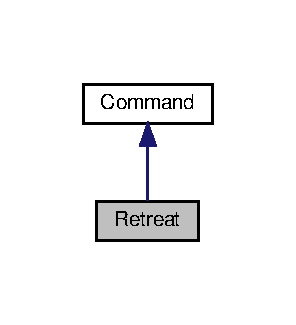
\includegraphics[width=142pt]{classRetreat__inherit__graph}
\end{center}
\end{figure}


Collaboration diagram for Retreat\+:\nopagebreak
\begin{figure}[H]
\begin{center}
\leavevmode
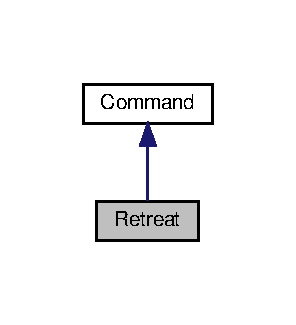
\includegraphics[width=142pt]{classRetreat__coll__graph}
\end{center}
\end{figure}
\subsection*{Public Member Functions}
\begin{DoxyCompactItemize}
\item 
\hyperlink{classRetreat_a889d73ed4b9fcdf13cfa986145d8763a}{Retreat} ()
\item 
void \hyperlink{classRetreat_a18fe7bf00ed623de02de5764b9607f5f}{execute} ()
\item 
\hyperlink{classRetreat_af14f96d3b46f7757511442c01f20edd9}{$\sim$\+Retreat} ()
\item 
\hyperlink{classRetreat_ab748f69c4ed3552908789bc18c73f917}{Retreat} (\hyperlink{classSpaceship}{Spaceship} $\ast$ship)
\end{DoxyCompactItemize}


\subsection{Detailed Description}
\hyperlink{classPlanet}{Planet} class. 

\subsection{Constructor \& Destructor Documentation}
\mbox{\Hypertarget{classRetreat_a889d73ed4b9fcdf13cfa986145d8763a}\label{classRetreat_a889d73ed4b9fcdf13cfa986145d8763a}} 
\index{Retreat@{Retreat}!Retreat@{Retreat}}
\index{Retreat@{Retreat}!Retreat@{Retreat}}
\subsubsection{\texorpdfstring{Retreat()}{Retreat()}\hspace{0.1cm}{\footnotesize\ttfamily [1/2]}}
{\footnotesize\ttfamily Retreat\+::\+Retreat (\begin{DoxyParamCaption}{ }\end{DoxyParamCaption})}

default constructor \mbox{\Hypertarget{classRetreat_af14f96d3b46f7757511442c01f20edd9}\label{classRetreat_af14f96d3b46f7757511442c01f20edd9}} 
\index{Retreat@{Retreat}!````~Retreat@{$\sim$\+Retreat}}
\index{````~Retreat@{$\sim$\+Retreat}!Retreat@{Retreat}}
\subsubsection{\texorpdfstring{$\sim$\+Retreat()}{~Retreat()}}
{\footnotesize\ttfamily Retreat\+::$\sim$\+Retreat (\begin{DoxyParamCaption}{ }\end{DoxyParamCaption})}

Default Destructor \mbox{\Hypertarget{classRetreat_ab748f69c4ed3552908789bc18c73f917}\label{classRetreat_ab748f69c4ed3552908789bc18c73f917}} 
\index{Retreat@{Retreat}!Retreat@{Retreat}}
\index{Retreat@{Retreat}!Retreat@{Retreat}}
\subsubsection{\texorpdfstring{Retreat()}{Retreat()}\hspace{0.1cm}{\footnotesize\ttfamily [2/2]}}
{\footnotesize\ttfamily Retreat\+::\+Retreat (\begin{DoxyParamCaption}\item[{\hyperlink{classSpaceship}{Spaceship} $\ast$}]{ship }\end{DoxyParamCaption})\hspace{0.3cm}{\ttfamily [inline]}}

Paramaterised constructor 
\begin{DoxyParams}{Parameters}
{\em ship} & \\
\hline
\end{DoxyParams}


\subsection{Member Function Documentation}
\mbox{\Hypertarget{classRetreat_a18fe7bf00ed623de02de5764b9607f5f}\label{classRetreat_a18fe7bf00ed623de02de5764b9607f5f}} 
\index{Retreat@{Retreat}!execute@{execute}}
\index{execute@{execute}!Retreat@{Retreat}}
\subsubsection{\texorpdfstring{execute()}{execute()}}
{\footnotesize\ttfamily void Retreat\+::execute (\begin{DoxyParamCaption}{ }\end{DoxyParamCaption})\hspace{0.3cm}{\ttfamily [virtual]}}

Execute Function That will call The Receivers action function 

Implements \hyperlink{classCommand_a6fd7d9bd8df8bfc881e4d6c7cd1878b7}{Command}.



The documentation for this class was generated from the following files\+:\begin{DoxyCompactItemize}
\item 
Retreat.\+h\item 
Retreat.\+cpp\end{DoxyCompactItemize}

\hypertarget{classSickBay}{}\section{Sick\+Bay Class Reference}
\label{classSickBay}\index{Sick\+Bay@{Sick\+Bay}}


Sickbay class.  




{\ttfamily \#include $<$Sick\+Bay.\+h$>$}



Inheritance diagram for Sick\+Bay\+:\nopagebreak
\begin{figure}[H]
\begin{center}
\leavevmode
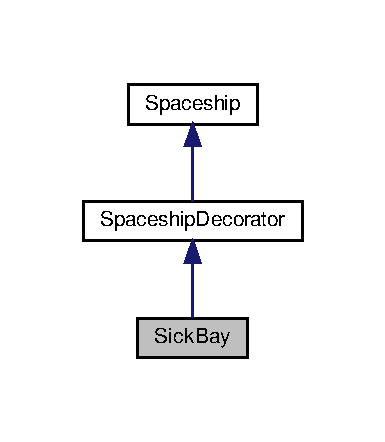
\includegraphics[width=185pt]{classSickBay__inherit__graph}
\end{center}
\end{figure}


Collaboration diagram for Sick\+Bay\+:\nopagebreak
\begin{figure}[H]
\begin{center}
\leavevmode
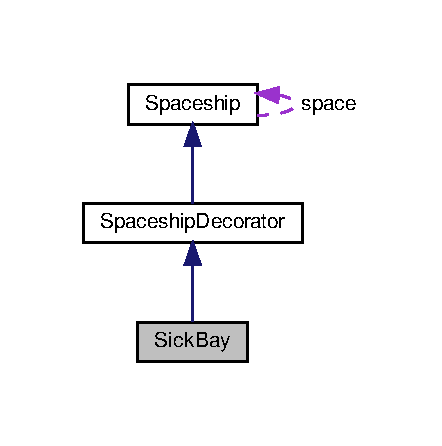
\includegraphics[width=212pt]{classSickBay__coll__graph}
\end{center}
\end{figure}
\subsection*{Public Member Functions}
\begin{DoxyCompactItemize}
\item 
\hyperlink{classSickBay_a6deba7260251b077d29cabb75587f9c6}{Sick\+Bay} ()
\item 
\hyperlink{classSickBay_a527219ede6b1a75938fef90ecc0b7755}{$\sim$\+Sick\+Bay} ()
\item 
void \hyperlink{classSickBay_aa70415a7714cdd88553f3694b3f2e9e1}{add\+Ship} (\hyperlink{classSpaceship}{Spaceship} $\ast$s)
\item 
void \hyperlink{classSickBay_a3934a1b821fbd192a946a9aff4575afa}{add\+Person} (\hyperlink{classPeople}{People} $\ast$p)
\item 
double \hyperlink{classSickBay_ab14fde02df1e95c352ba51d59480c3fa}{get\+Resources} (double a, double b)
\item 
void \hyperlink{classSickBay_a4f8395f68f93b62e0cc68f6a3bd3af79}{visit} (\hyperlink{classPlanet}{Planet} $\ast$p)
\item 
\hyperlink{classMemento}{Memento} $\ast$ \hyperlink{classSickBay_a0d06ca126941dae25aaf74838dd1914b}{create\+Memento} (vector$<$ \hyperlink{classSpaceship}{Spaceship} $\ast$$>$ s)
\item 
void \hyperlink{classSickBay_a1b2156dee5ed14c68c3f25ee3a53e9c8}{reinstate\+Memento} (\hyperlink{classMemento}{Memento} $\ast$mem)
\item 
void \hyperlink{classSickBay_af053a3507f8246fd1577124644cf7477}{execute\+Strategy} ()
\item 
void \hyperlink{classSickBay_ac25920ac3e757e289ea25233991fa94e}{select\+Strategy} (\hyperlink{classStrategy}{Strategy} $\ast$s)
\end{DoxyCompactItemize}
\subsection*{Additional Inherited Members}


\subsection{Detailed Description}
Sickbay class. 

\subsection{Constructor \& Destructor Documentation}
\mbox{\Hypertarget{classSickBay_a6deba7260251b077d29cabb75587f9c6}\label{classSickBay_a6deba7260251b077d29cabb75587f9c6}} 
\index{Sick\+Bay@{Sick\+Bay}!Sick\+Bay@{Sick\+Bay}}
\index{Sick\+Bay@{Sick\+Bay}!Sick\+Bay@{Sick\+Bay}}
\subsubsection{\texorpdfstring{Sick\+Bay()}{SickBay()}}
{\footnotesize\ttfamily Sick\+Bay\+::\+Sick\+Bay (\begin{DoxyParamCaption}{ }\end{DoxyParamCaption})}

Default constructor \mbox{\Hypertarget{classSickBay_a527219ede6b1a75938fef90ecc0b7755}\label{classSickBay_a527219ede6b1a75938fef90ecc0b7755}} 
\index{Sick\+Bay@{Sick\+Bay}!````~Sick\+Bay@{$\sim$\+Sick\+Bay}}
\index{````~Sick\+Bay@{$\sim$\+Sick\+Bay}!Sick\+Bay@{Sick\+Bay}}
\subsubsection{\texorpdfstring{$\sim$\+Sick\+Bay()}{~SickBay()}}
{\footnotesize\ttfamily Sick\+Bay\+::$\sim$\+Sick\+Bay (\begin{DoxyParamCaption}{ }\end{DoxyParamCaption})}

Default desctructor 

\subsection{Member Function Documentation}
\mbox{\Hypertarget{classSickBay_a3934a1b821fbd192a946a9aff4575afa}\label{classSickBay_a3934a1b821fbd192a946a9aff4575afa}} 
\index{Sick\+Bay@{Sick\+Bay}!add\+Person@{add\+Person}}
\index{add\+Person@{add\+Person}!Sick\+Bay@{Sick\+Bay}}
\subsubsection{\texorpdfstring{add\+Person()}{addPerson()}}
{\footnotesize\ttfamily void Sick\+Bay\+::add\+Person (\begin{DoxyParamCaption}\item[{\hyperlink{classPeople}{People} $\ast$}]{p }\end{DoxyParamCaption})\hspace{0.3cm}{\ttfamily [inline]}, {\ttfamily [virtual]}}

stub for add\+Person 

Reimplemented from \hyperlink{classSpaceshipDecorator_a6e289d8a65f35b9f223255ae0eaa3b00}{Spaceship\+Decorator}.

\mbox{\Hypertarget{classSickBay_aa70415a7714cdd88553f3694b3f2e9e1}\label{classSickBay_aa70415a7714cdd88553f3694b3f2e9e1}} 
\index{Sick\+Bay@{Sick\+Bay}!add\+Ship@{add\+Ship}}
\index{add\+Ship@{add\+Ship}!Sick\+Bay@{Sick\+Bay}}
\subsubsection{\texorpdfstring{add\+Ship()}{addShip()}}
{\footnotesize\ttfamily void Sick\+Bay\+::add\+Ship (\begin{DoxyParamCaption}\item[{\hyperlink{classSpaceship}{Spaceship} $\ast$}]{s }\end{DoxyParamCaption})\hspace{0.3cm}{\ttfamily [inline]}, {\ttfamily [virtual]}}

Virtual add\+Ship 

Reimplemented from \hyperlink{classSpaceshipDecorator_a5ed39419f5fab65dd4af11bf5136f7a4}{Spaceship\+Decorator}.

\mbox{\Hypertarget{classSickBay_a0d06ca126941dae25aaf74838dd1914b}\label{classSickBay_a0d06ca126941dae25aaf74838dd1914b}} 
\index{Sick\+Bay@{Sick\+Bay}!create\+Memento@{create\+Memento}}
\index{create\+Memento@{create\+Memento}!Sick\+Bay@{Sick\+Bay}}
\subsubsection{\texorpdfstring{create\+Memento()}{createMemento()}}
{\footnotesize\ttfamily \hyperlink{classMemento}{Memento}$\ast$ Sick\+Bay\+::create\+Memento (\begin{DoxyParamCaption}\item[{vector$<$ \hyperlink{classSpaceship}{Spaceship} $\ast$$>$}]{s }\end{DoxyParamCaption})\hspace{0.3cm}{\ttfamily [inline]}, {\ttfamily [virtual]}}

create memento stub 

Reimplemented from \hyperlink{classSpaceship_a6d272f846b019dec8226ddab65648a7b}{Spaceship}.

\mbox{\Hypertarget{classSickBay_af053a3507f8246fd1577124644cf7477}\label{classSickBay_af053a3507f8246fd1577124644cf7477}} 
\index{Sick\+Bay@{Sick\+Bay}!execute\+Strategy@{execute\+Strategy}}
\index{execute\+Strategy@{execute\+Strategy}!Sick\+Bay@{Sick\+Bay}}
\subsubsection{\texorpdfstring{execute\+Strategy()}{executeStrategy()}}
{\footnotesize\ttfamily void Sick\+Bay\+::execute\+Strategy (\begin{DoxyParamCaption}{ }\end{DoxyParamCaption})\hspace{0.3cm}{\ttfamily [inline]}, {\ttfamily [virtual]}}

execute strategy 

Reimplemented from \hyperlink{classSpaceship}{Spaceship}.

\mbox{\Hypertarget{classSickBay_ab14fde02df1e95c352ba51d59480c3fa}\label{classSickBay_ab14fde02df1e95c352ba51d59480c3fa}} 
\index{Sick\+Bay@{Sick\+Bay}!get\+Resources@{get\+Resources}}
\index{get\+Resources@{get\+Resources}!Sick\+Bay@{Sick\+Bay}}
\subsubsection{\texorpdfstring{get\+Resources()}{getResources()}}
{\footnotesize\ttfamily double Sick\+Bay\+::get\+Resources (\begin{DoxyParamCaption}\item[{double}]{a,  }\item[{double}]{b }\end{DoxyParamCaption})\hspace{0.3cm}{\ttfamily [inline]}, {\ttfamily [virtual]}}

stub resource collection 

Reimplemented from \hyperlink{classSpaceshipDecorator_a5ee7a9a8c146c85f08591e47d971dce7}{Spaceship\+Decorator}.

\mbox{\Hypertarget{classSickBay_a1b2156dee5ed14c68c3f25ee3a53e9c8}\label{classSickBay_a1b2156dee5ed14c68c3f25ee3a53e9c8}} 
\index{Sick\+Bay@{Sick\+Bay}!reinstate\+Memento@{reinstate\+Memento}}
\index{reinstate\+Memento@{reinstate\+Memento}!Sick\+Bay@{Sick\+Bay}}
\subsubsection{\texorpdfstring{reinstate\+Memento()}{reinstateMemento()}}
{\footnotesize\ttfamily void Sick\+Bay\+::reinstate\+Memento (\begin{DoxyParamCaption}\item[{\hyperlink{classMemento}{Memento} $\ast$}]{mem }\end{DoxyParamCaption})\hspace{0.3cm}{\ttfamily [inline]}, {\ttfamily [virtual]}}

reinstate memento 

Reimplemented from \hyperlink{classSpaceship_ab075c869473344b6471c8e28ca7ea61e}{Spaceship}.

\mbox{\Hypertarget{classSickBay_ac25920ac3e757e289ea25233991fa94e}\label{classSickBay_ac25920ac3e757e289ea25233991fa94e}} 
\index{Sick\+Bay@{Sick\+Bay}!select\+Strategy@{select\+Strategy}}
\index{select\+Strategy@{select\+Strategy}!Sick\+Bay@{Sick\+Bay}}
\subsubsection{\texorpdfstring{select\+Strategy()}{selectStrategy()}}
{\footnotesize\ttfamily void Sick\+Bay\+::select\+Strategy (\begin{DoxyParamCaption}\item[{\hyperlink{classStrategy}{Strategy} $\ast$}]{s }\end{DoxyParamCaption})\hspace{0.3cm}{\ttfamily [inline]}, {\ttfamily [virtual]}}

select strategy 

Reimplemented from \hyperlink{classSpaceship_a93be2d9d2b675ef978d866d4cd7a6524}{Spaceship}.

\mbox{\Hypertarget{classSickBay_a4f8395f68f93b62e0cc68f6a3bd3af79}\label{classSickBay_a4f8395f68f93b62e0cc68f6a3bd3af79}} 
\index{Sick\+Bay@{Sick\+Bay}!visit@{visit}}
\index{visit@{visit}!Sick\+Bay@{Sick\+Bay}}
\subsubsection{\texorpdfstring{visit()}{visit()}}
{\footnotesize\ttfamily void Sick\+Bay\+::visit (\begin{DoxyParamCaption}\item[{\hyperlink{classPlanet}{Planet} $\ast$}]{p }\end{DoxyParamCaption})\hspace{0.3cm}{\ttfamily [inline]}, {\ttfamily [virtual]}}

stub for visit 

Reimplemented from \hyperlink{classSpaceship}{Spaceship}.



The documentation for this class was generated from the following files\+:\begin{DoxyCompactItemize}
\item 
Sick\+Bay.\+h\item 
Sick\+Bay.\+cpp\end{DoxyCompactItemize}

\hypertarget{classSleepingQuarters}{}\section{Sleeping\+Quarters Class Reference}
\label{classSleepingQuarters}\index{Sleeping\+Quarters@{Sleeping\+Quarters}}


Sleeping quarters class.  




{\ttfamily \#include $<$Sleeping\+Quarters.\+h$>$}



Inheritance diagram for Sleeping\+Quarters\+:
% FIG 0


Collaboration diagram for Sleeping\+Quarters\+:
% FIG 1
\subsection*{Public Member Functions}
\begin{DoxyCompactItemize}
\item 
\hyperlink{classSleepingQuarters_ab4055fa9d6ac27506b1577faec404fbb}{Sleeping\+Quarters} ()
\item 
\hyperlink{classSleepingQuarters_ad32e286540e322186993b15f5ebcffbc}{$\sim$\+Sleeping\+Quarters} ()
\end{DoxyCompactItemize}
\subsection*{Additional Inherited Members}


\subsection{Detailed Description}
Sleeping quarters class. 

\subsection{Constructor \& Destructor Documentation}
\mbox{\Hypertarget{classSleepingQuarters_ab4055fa9d6ac27506b1577faec404fbb}\label{classSleepingQuarters_ab4055fa9d6ac27506b1577faec404fbb}} 
\index{Sleeping\+Quarters@{Sleeping\+Quarters}!Sleeping\+Quarters@{Sleeping\+Quarters}}
\index{Sleeping\+Quarters@{Sleeping\+Quarters}!Sleeping\+Quarters@{Sleeping\+Quarters}}
\subsubsection{\texorpdfstring{Sleeping\+Quarters()}{SleepingQuarters()}}
{\footnotesize\ttfamily Sleeping\+Quarters\+::\+Sleeping\+Quarters (\begin{DoxyParamCaption}{ }\end{DoxyParamCaption})}

default constructor \mbox{\Hypertarget{classSleepingQuarters_ad32e286540e322186993b15f5ebcffbc}\label{classSleepingQuarters_ad32e286540e322186993b15f5ebcffbc}} 
\index{Sleeping\+Quarters@{Sleeping\+Quarters}!````~Sleeping\+Quarters@{$\sim$\+Sleeping\+Quarters}}
\index{````~Sleeping\+Quarters@{$\sim$\+Sleeping\+Quarters}!Sleeping\+Quarters@{Sleeping\+Quarters}}
\subsubsection{\texorpdfstring{$\sim$\+Sleeping\+Quarters()}{~SleepingQuarters()}}
{\footnotesize\ttfamily Sleeping\+Quarters\+::$\sim$\+Sleeping\+Quarters (\begin{DoxyParamCaption}{ }\end{DoxyParamCaption})}

default desctructor 

The documentation for this class was generated from the following files\+:\begin{DoxyCompactItemize}
\item 
Sleeping\+Quarters.\+h\item 
Sleeping\+Quarters.\+cpp\end{DoxyCompactItemize}

\hypertarget{classSpaceship}{}\section{Spaceship Class Reference}
\label{classSpaceship}\index{Spaceship@{Spaceship}}


\hyperlink{classSpaceship}{Spaceship} class.  




{\ttfamily \#include $<$Spaceship.\+h$>$}



Inheritance diagram for Spaceship\+:\nopagebreak
\begin{figure}[H]
\begin{center}
\leavevmode
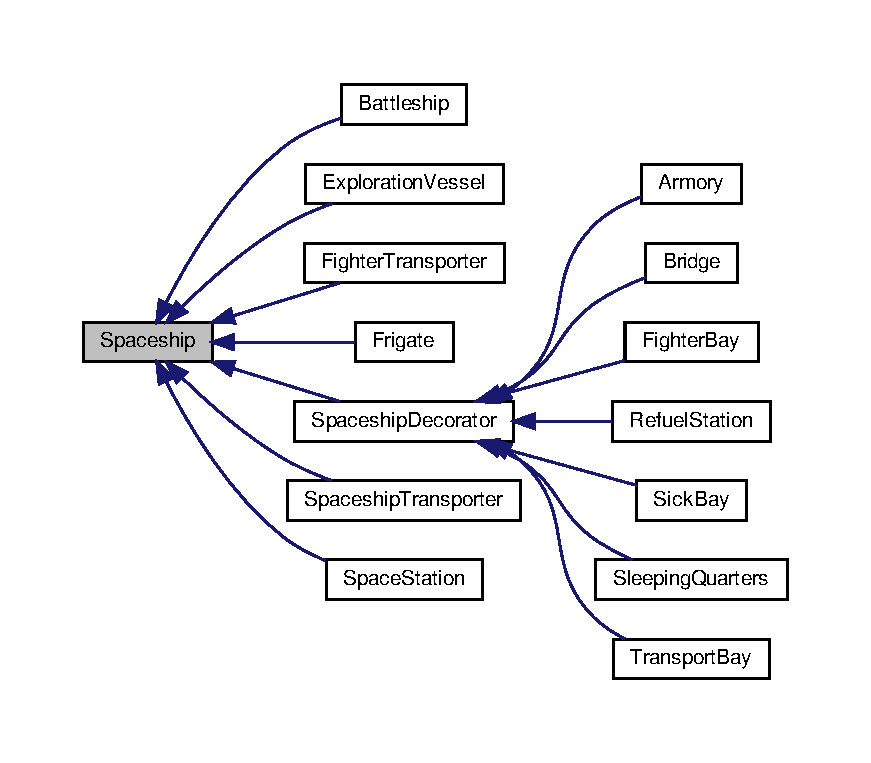
\includegraphics[width=350pt]{classSpaceship__inherit__graph}
\end{center}
\end{figure}


Collaboration diagram for Spaceship\+:\nopagebreak
\begin{figure}[H]
\begin{center}
\leavevmode
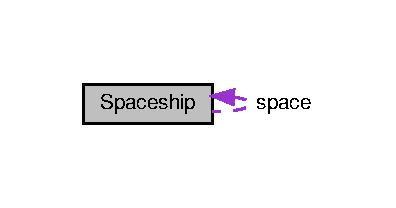
\includegraphics[width=190pt]{classSpaceship__coll__graph}
\end{center}
\end{figure}
\subsection*{Public Member Functions}
\begin{DoxyCompactItemize}
\item 
\hyperlink{classSpaceship_a13f1c8eb5ded2fb1687203322b22bca9}{Spaceship} ()
\item 
\hyperlink{classSpaceship_a27d48c8aff00407fd50f18522aa5164c}{Spaceship} (string n)
\item 
virtual void \hyperlink{classSpaceship_ac1b4673a691cd100708ddea08cd9f192}{add\+Component} (\hyperlink{classSpaceship}{Spaceship} $\ast$)=0
\item 
virtual \hyperlink{classSpaceship_aaf51352795ea2382e2aaea4b9a058804}{$\sim$\+Spaceship} ()
\item 
\mbox{\Hypertarget{classSpaceship_a5c2741aa19fc4f38c1507b7c266fad1b}\label{classSpaceship_a5c2741aa19fc4f38c1507b7c266fad1b}} 
int {\bfseries get\+Displacement} ()
\item 
\mbox{\Hypertarget{classSpaceship_a689b09969d583d03adcb34073338395a}\label{classSpaceship_a689b09969d583d03adcb34073338395a}} 
void {\bfseries set\+Displacement} (int d)
\item 
\mbox{\Hypertarget{classSpaceship_a4085ec55d3c13c8ba5f63bd8dee4573e}\label{classSpaceship_a4085ec55d3c13c8ba5f63bd8dee4573e}} 
int {\bfseries get\+Power} ()
\item 
\mbox{\Hypertarget{classSpaceship_ae9697723e1b398c6531a0f48a3145c02}\label{classSpaceship_ae9697723e1b398c6531a0f48a3145c02}} 
void {\bfseries set\+Power} (int v)
\item 
\mbox{\Hypertarget{classSpaceship_a080ecccde68594817833a3d62e7f63f0}\label{classSpaceship_a080ecccde68594817833a3d62e7f63f0}} 
int {\bfseries get\+Thrust} ()
\item 
\mbox{\Hypertarget{classSpaceship_a2983f2dc9719e86ac19bdcd12b368f1d}\label{classSpaceship_a2983f2dc9719e86ac19bdcd12b368f1d}} 
void {\bfseries set\+Thrust} (int v)
\item 
\mbox{\Hypertarget{classSpaceship_a6d16c208dc343fef047faf23ae1b0d9e}\label{classSpaceship_a6d16c208dc343fef047faf23ae1b0d9e}} 
int {\bfseries get\+Max\+Speed} ()
\item 
\mbox{\Hypertarget{classSpaceship_a81b89e1e8d798bc3de8140f0d37092b1}\label{classSpaceship_a81b89e1e8d798bc3de8140f0d37092b1}} 
void {\bfseries set\+Max\+Speed} (int v)
\item 
\mbox{\Hypertarget{classSpaceship_a60b2e50a33df60c62a712d30b0b75d76}\label{classSpaceship_a60b2e50a33df60c62a712d30b0b75d76}} 
int {\bfseries get\+Stall\+Speed} ()
\item 
\mbox{\Hypertarget{classSpaceship_a8bd8be2516ced3b5794b32d6feefb49a}\label{classSpaceship_a8bd8be2516ced3b5794b32d6feefb49a}} 
void {\bfseries set\+Stall\+Speed} (int v)
\item 
\mbox{\Hypertarget{classSpaceship_aa914585a0da2052040e1f04195d55b07}\label{classSpaceship_aa914585a0da2052040e1f04195d55b07}} 
int {\bfseries get\+Current\+Capacity} ()
\item 
\mbox{\Hypertarget{classSpaceship_a788f0adef62986c451acb9e47ed0323e}\label{classSpaceship_a788f0adef62986c451acb9e47ed0323e}} 
void {\bfseries set\+Current\+Capacity} (int p)
\item 
\mbox{\Hypertarget{classSpaceship_a38e2edec47ed44841ab62410eb419a87}\label{classSpaceship_a38e2edec47ed44841ab62410eb419a87}} 
int {\bfseries get\+Passenger\+Capacity} ()
\item 
\mbox{\Hypertarget{classSpaceship_adc52ae78b60490cad9f91f56ee1557f0}\label{classSpaceship_adc52ae78b60490cad9f91f56ee1557f0}} 
void {\bfseries set\+Passenger\+Capacity} (int p)
\item 
\mbox{\Hypertarget{classSpaceship_ac91b941c399543479336b837ba8dc286}\label{classSpaceship_ac91b941c399543479336b837ba8dc286}} 
int {\bfseries get\+Max\+Fuel} ()
\item 
\mbox{\Hypertarget{classSpaceship_ac81cea3a321263e3fa162c8435c49d9d}\label{classSpaceship_ac81cea3a321263e3fa162c8435c49d9d}} 
void {\bfseries set\+Max\+Fuel} (int i)
\item 
\mbox{\Hypertarget{classSpaceship_afa3be0e2d9d397ba4ffda36047be8939}\label{classSpaceship_afa3be0e2d9d397ba4ffda36047be8939}} 
void {\bfseries add\+Fuel} (int a)
\item 
\mbox{\Hypertarget{classSpaceship_a409d73f889bce7b8772eeff17b04a965}\label{classSpaceship_a409d73f889bce7b8772eeff17b04a965}} 
void {\bfseries add\+Energy} (int e)
\item 
\mbox{\Hypertarget{classSpaceship_a14bc1b626e87d340cd8c53faf47b892f}\label{classSpaceship_a14bc1b626e87d340cd8c53faf47b892f}} 
void {\bfseries decrease\+Fuel} (int a)
\item 
\mbox{\Hypertarget{classSpaceship_a042c3a5a6dddbfa2db3d411baf3f3f9f}\label{classSpaceship_a042c3a5a6dddbfa2db3d411baf3f3f9f}} 
void {\bfseries decrease\+Energy} (int e)
\item 
\mbox{\Hypertarget{classSpaceship_afa03d65f0166d453527e2eb595426ab5}\label{classSpaceship_afa03d65f0166d453527e2eb595426ab5}} 
int {\bfseries get\+Fuel} ()
\item 
\mbox{\Hypertarget{classSpaceship_ad28625e31d78cc1edb5e248aaf3f01d8}\label{classSpaceship_ad28625e31d78cc1edb5e248aaf3f01d8}} 
int {\bfseries get\+Energy} ()
\item 
\mbox{\Hypertarget{classSpaceship_a89441170fc458252bf8fad377683c23d}\label{classSpaceship_a89441170fc458252bf8fad377683c23d}} 
string {\bfseries get\+Name} ()
\item 
virtual void \hyperlink{classSpaceship_a5ddf702124286d9d3a6b5e64c09515bc}{increase\+Threat\+Level} ()
\item 
virtual void \hyperlink{classSpaceship_a73a1eefd211e9a2063d924ee85f0c0c7}{decrease\+Threat\+Level} ()
\item 
virtual void \hyperlink{classSpaceship_a8f16814f888a5a1423e5a491329cdb97}{print\+Threat\+Level} ()
\item 
\mbox{\Hypertarget{classSpaceship_add79868aef85232b23c04af06f288447}\label{classSpaceship_add79868aef85232b23c04af06f288447}} 
virtual void {\bfseries visit} (\hyperlink{classPlanet}{Planet} $\ast$p)
\item 
\mbox{\Hypertarget{classSpaceship_a10e76fb093ab448894cdeb70994c821d}\label{classSpaceship_a10e76fb093ab448894cdeb70994c821d}} 
virtual void {\bfseries execute\+Strategy} ()
\item 
virtual void \hyperlink{classSpaceship_a93be2d9d2b675ef978d866d4cd7a6524}{select\+Strategy} (\hyperlink{classStrategy}{Strategy} $\ast$s)
\item 
virtual void \hyperlink{classSpaceship_a67b7e60d2dc77e740309a9d994d653a1}{add\+Passenger} (\hyperlink{classPeople}{People} $\ast$)
\item 
virtual void \hyperlink{classSpaceship_ac816c2990b25a1b7c9f6acbc9ca132ee}{remove\+Passenger} (\hyperlink{classPeople}{People} $\ast$)
\item 
virtual int \hyperlink{classSpaceship_a3ed78b14953957576e42c6e741e04690}{enter\+Ship} (\hyperlink{classPeople}{People} $\ast$)
\item 
virtual void \hyperlink{classSpaceship_ae3ddb55d813fa2a3454c1745b23cf6ef}{exit\+Ship} (int)
\item 
void \hyperlink{classSpaceship_a6539b155cc0dc525c506eee788fe9449}{broadcast} (string)
\item 
void \hyperlink{classSpaceship_a949e9815b99d5598da2239e307036141}{print\+Captains\+Log} ()
\item 
void \hyperlink{classSpaceship_acf25a335848231435a64a484c103dfcb}{add\+Log} (string)
\item 
virtual int \hyperlink{classSpaceship_a113055e6d793f8fbc55e44efc4d57e07}{get\+Type} ()
\item 
vector$<$ \hyperlink{classPeople}{People} $\ast$ $>$ \hyperlink{classSpaceship_a23155ea96d499b31bde27e0c2f704ae6}{get\+People} ()
\item 
virtual void \hyperlink{classSpaceship_a90e1321cdbcb459b98b75ab39cef867d}{add\+Ship} (\hyperlink{classSpaceship}{Spaceship} $\ast$)
\item 
virtual double \hyperlink{classSpaceship_ad2027533de1d789db5e3efa22055f2d0}{get\+Resources} (double a, double b)
\item 
virtual void \hyperlink{classSpaceship_add8d9c6dfd5f6ecb8399e41e71e5b22f}{add\+Person} (\hyperlink{classPeople}{People} $\ast$p)
\item 
\mbox{\Hypertarget{classSpaceship_a0738743f89a841847605c3262a822183}\label{classSpaceship_a0738743f89a841847605c3262a822183}} 
virtual void {\bfseries visit} (\hyperlink{classPeople}{People} $\ast$p)
\item 
virtual \hyperlink{classMemento}{Memento} $\ast$ \hyperlink{classSpaceship_a6d272f846b019dec8226ddab65648a7b}{create\+Memento} (vector$<$ \hyperlink{classSpaceship}{Spaceship} $\ast$$>$ s)
\item 
virtual void \hyperlink{classSpaceship_ab075c869473344b6471c8e28ca7ea61e}{reinstate\+Memento} (\hyperlink{classMemento}{Memento} $\ast$mem)
\end{DoxyCompactItemize}
\subsection*{Protected Attributes}
\begin{DoxyCompactItemize}
\item 
\hyperlink{classSpaceship}{Spaceship} $\ast$ \hyperlink{classSpaceship_a0f53795d5f23cc37369cea2e52bd70b1}{space}
\end{DoxyCompactItemize}


\subsection{Detailed Description}
\hyperlink{classSpaceship}{Spaceship} class. 

\subsection{Constructor \& Destructor Documentation}
\mbox{\Hypertarget{classSpaceship_a13f1c8eb5ded2fb1687203322b22bca9}\label{classSpaceship_a13f1c8eb5ded2fb1687203322b22bca9}} 
\index{Spaceship@{Spaceship}!Spaceship@{Spaceship}}
\index{Spaceship@{Spaceship}!Spaceship@{Spaceship}}
\subsubsection{\texorpdfstring{Spaceship()}{Spaceship()}\hspace{0.1cm}{\footnotesize\ttfamily [1/2]}}
{\footnotesize\ttfamily Spaceship\+::\+Spaceship (\begin{DoxyParamCaption}{ }\end{DoxyParamCaption})\hspace{0.3cm}{\ttfamily [inline]}}

default constructor \mbox{\Hypertarget{classSpaceship_a27d48c8aff00407fd50f18522aa5164c}\label{classSpaceship_a27d48c8aff00407fd50f18522aa5164c}} 
\index{Spaceship@{Spaceship}!Spaceship@{Spaceship}}
\index{Spaceship@{Spaceship}!Spaceship@{Spaceship}}
\subsubsection{\texorpdfstring{Spaceship()}{Spaceship()}\hspace{0.1cm}{\footnotesize\ttfamily [2/2]}}
{\footnotesize\ttfamily Spaceship\+::\+Spaceship (\begin{DoxyParamCaption}\item[{string}]{n }\end{DoxyParamCaption})\hspace{0.3cm}{\ttfamily [inline]}}

Paramaterised constructor \mbox{\Hypertarget{classSpaceship_aaf51352795ea2382e2aaea4b9a058804}\label{classSpaceship_aaf51352795ea2382e2aaea4b9a058804}} 
\index{Spaceship@{Spaceship}!````~Spaceship@{$\sim$\+Spaceship}}
\index{````~Spaceship@{$\sim$\+Spaceship}!Spaceship@{Spaceship}}
\subsubsection{\texorpdfstring{$\sim$\+Spaceship()}{~Spaceship()}}
{\footnotesize\ttfamily virtual Spaceship\+::$\sim$\+Spaceship (\begin{DoxyParamCaption}{ }\end{DoxyParamCaption})\hspace{0.3cm}{\ttfamily [inline]}, {\ttfamily [virtual]}}

Default desctructor 

\subsection{Member Function Documentation}
\mbox{\Hypertarget{classSpaceship_ac1b4673a691cd100708ddea08cd9f192}\label{classSpaceship_ac1b4673a691cd100708ddea08cd9f192}} 
\index{Spaceship@{Spaceship}!add\+Component@{add\+Component}}
\index{add\+Component@{add\+Component}!Spaceship@{Spaceship}}
\subsubsection{\texorpdfstring{add\+Component()}{addComponent()}}
{\footnotesize\ttfamily virtual void Spaceship\+::add\+Component (\begin{DoxyParamCaption}\item[{\hyperlink{classSpaceship}{Spaceship} $\ast$}]{ }\end{DoxyParamCaption})\hspace{0.3cm}{\ttfamily [pure virtual]}}

Pure virtual method for decorator to add components to the spaceship 

Implemented in \hyperlink{classSpaceshipTransporter_acd55c6864eab86db5e0485beeec4e8b9}{Spaceship\+Transporter}, \hyperlink{classSpaceStation_ae89449fdcf5d44229fb93a14fc496fe1}{Space\+Station}, \hyperlink{classFighterTransporter_a962db4e241d764360407380ce1438788}{Fighter\+Transporter}, \hyperlink{classExplorationVessel_ae952e198a28fd0a5ec998ecdcca86561}{Exploration\+Vessel}, \hyperlink{classBattleship_a698e2d0ef1ffa4e6b5e7b09c0ff7d07c}{Battleship}, \hyperlink{classFrigate_af1c809e79096219e53da2f577ec8178d}{Frigate}, and \hyperlink{classSpaceshipDecorator_a08442441af1fa8979f1e411a5e7b511c}{Spaceship\+Decorator}.

\mbox{\Hypertarget{classSpaceship_acf25a335848231435a64a484c103dfcb}\label{classSpaceship_acf25a335848231435a64a484c103dfcb}} 
\index{Spaceship@{Spaceship}!add\+Log@{add\+Log}}
\index{add\+Log@{add\+Log}!Spaceship@{Spaceship}}
\subsubsection{\texorpdfstring{add\+Log()}{addLog()}}
{\footnotesize\ttfamily void Spaceship\+::add\+Log (\begin{DoxyParamCaption}\item[{string}]{message }\end{DoxyParamCaption})}

Add message to the log 
\begin{DoxyParams}{Parameters}
{\em message} & -\/ message to added to log \\
\hline
\end{DoxyParams}
\mbox{\Hypertarget{classSpaceship_a67b7e60d2dc77e740309a9d994d653a1}\label{classSpaceship_a67b7e60d2dc77e740309a9d994d653a1}} 
\index{Spaceship@{Spaceship}!add\+Passenger@{add\+Passenger}}
\index{add\+Passenger@{add\+Passenger}!Spaceship@{Spaceship}}
\subsubsection{\texorpdfstring{add\+Passenger()}{addPassenger()}}
{\footnotesize\ttfamily void Spaceship\+::add\+Passenger (\begin{DoxyParamCaption}\item[{\hyperlink{classPeople}{People} $\ast$}]{p }\end{DoxyParamCaption})\hspace{0.3cm}{\ttfamily [virtual]}}

Add passenger to spaceship 
\begin{DoxyParams}{Parameters}
{\em p} & -\/ Person to be added \\
\hline
\end{DoxyParams}
\mbox{\Hypertarget{classSpaceship_add8d9c6dfd5f6ecb8399e41e71e5b22f}\label{classSpaceship_add8d9c6dfd5f6ecb8399e41e71e5b22f}} 
\index{Spaceship@{Spaceship}!add\+Person@{add\+Person}}
\index{add\+Person@{add\+Person}!Spaceship@{Spaceship}}
\subsubsection{\texorpdfstring{add\+Person()}{addPerson()}}
{\footnotesize\ttfamily virtual void Spaceship\+::add\+Person (\begin{DoxyParamCaption}\item[{\hyperlink{classPeople}{People} $\ast$}]{p }\end{DoxyParamCaption})\hspace{0.3cm}{\ttfamily [inline]}, {\ttfamily [virtual]}}

virtual add\+Person 

Reimplemented in \hyperlink{classFrigate_a5da866e084d1d07363f06ff052005b41}{Frigate}, \hyperlink{classSpaceStation_a46146c02fcd8107eda2972cc5843afd8}{Space\+Station}, \hyperlink{classExplorationVessel_a7be654e42a9e83800abfb897d9b308b8}{Exploration\+Vessel}, \hyperlink{classTransportBay_a2be08f6085583ec9f839ff8939c6a6b7}{Transport\+Bay}, \hyperlink{classSpaceshipTransporter_a5c9ee82688e97545baa7a876e69d5dd3}{Spaceship\+Transporter}, \hyperlink{classFighterBay_aa0777fe7c8a3e6b772fc8bf58a3cb9bb}{Fighter\+Bay}, \hyperlink{classFighterTransporter_a79b9099ea2cbdd17d1a0d6c8122e9bfa}{Fighter\+Transporter}, \hyperlink{classRefuelStation_a6bd40214cf5dc4d46739943f545c6d7a}{Refuel\+Station}, \hyperlink{classBridge_aec10bfb9af885933640548b509144a29}{Bridge}, \hyperlink{classSleepingQuarters_addd107a8005b61d51846e8e955922d50}{Sleeping\+Quarters}, \hyperlink{classSpaceshipDecorator_a6e289d8a65f35b9f223255ae0eaa3b00}{Spaceship\+Decorator}, and \hyperlink{classSickBay_a3934a1b821fbd192a946a9aff4575afa}{Sick\+Bay}.

\mbox{\Hypertarget{classSpaceship_a90e1321cdbcb459b98b75ab39cef867d}\label{classSpaceship_a90e1321cdbcb459b98b75ab39cef867d}} 
\index{Spaceship@{Spaceship}!add\+Ship@{add\+Ship}}
\index{add\+Ship@{add\+Ship}!Spaceship@{Spaceship}}
\subsubsection{\texorpdfstring{add\+Ship()}{addShip()}}
{\footnotesize\ttfamily virtual void Spaceship\+::add\+Ship (\begin{DoxyParamCaption}\item[{\hyperlink{classSpaceship}{Spaceship} $\ast$}]{ }\end{DoxyParamCaption})\hspace{0.3cm}{\ttfamily [inline]}, {\ttfamily [virtual]}}

Virtual add\+Ship 

Reimplemented in \hyperlink{classSpaceStation_ace2d37733fa5af9551aba31bc9229ad3}{Space\+Station}, \hyperlink{classExplorationVessel_ac6bc6807891edf928fae68e7ed850d14}{Exploration\+Vessel}, \hyperlink{classBattleship_a9167350d564a8f8286841408f0bacdf9}{Battleship}, \hyperlink{classFighterTransporter_ae4191358a54d0f30476beea30aa16317}{Fighter\+Transporter}, \hyperlink{classFrigate_a000802431ba3db8b45bfa6e7ae153de4}{Frigate}, \hyperlink{classSpaceshipTransporter_a493a4ba44d26a2ae4e85b79e6970fb91}{Spaceship\+Transporter}, \hyperlink{classFighterBay_a8975b88b27663c76f82168752593ceda}{Fighter\+Bay}, \hyperlink{classTransportBay_acd6b5b09e81bd28c6dcbe23d561fd99c}{Transport\+Bay}, \hyperlink{classBridge_a49676496d07502909958e747ef4c3214}{Bridge}, \hyperlink{classRefuelStation_a03510ee8365b5095ca80fac0c5a0a780}{Refuel\+Station}, \hyperlink{classSpaceshipDecorator_a5ed39419f5fab65dd4af11bf5136f7a4}{Spaceship\+Decorator}, \hyperlink{classArmory_adccb51a0901294546bfb1da350ae6836}{Armory}, \hyperlink{classSleepingQuarters_ae15ba2bf6be5cc0d4580da9ecbbe28f5}{Sleeping\+Quarters}, and \hyperlink{classSickBay_aa70415a7714cdd88553f3694b3f2e9e1}{Sick\+Bay}.

\mbox{\Hypertarget{classSpaceship_a6539b155cc0dc525c506eee788fe9449}\label{classSpaceship_a6539b155cc0dc525c506eee788fe9449}} 
\index{Spaceship@{Spaceship}!broadcast@{broadcast}}
\index{broadcast@{broadcast}!Spaceship@{Spaceship}}
\subsubsection{\texorpdfstring{broadcast()}{broadcast()}}
{\footnotesize\ttfamily void Spaceship\+::broadcast (\begin{DoxyParamCaption}\item[{string}]{message }\end{DoxyParamCaption})}

Broadcast message to passenger 
\begin{DoxyParams}{Parameters}
{\em message} & -\/ message to be broadcast \\
\hline
\end{DoxyParams}
\mbox{\Hypertarget{classSpaceship_a6d272f846b019dec8226ddab65648a7b}\label{classSpaceship_a6d272f846b019dec8226ddab65648a7b}} 
\index{Spaceship@{Spaceship}!create\+Memento@{create\+Memento}}
\index{create\+Memento@{create\+Memento}!Spaceship@{Spaceship}}
\subsubsection{\texorpdfstring{create\+Memento()}{createMemento()}}
{\footnotesize\ttfamily virtual \hyperlink{classMemento}{Memento}$\ast$ Spaceship\+::create\+Memento (\begin{DoxyParamCaption}\item[{vector$<$ \hyperlink{classSpaceship}{Spaceship} $\ast$$>$}]{s }\end{DoxyParamCaption})\hspace{0.3cm}{\ttfamily [inline]}, {\ttfamily [virtual]}}

create memento stub 

Reimplemented in \hyperlink{classSpaceStation_a7396c4080f29ca9c20975f831008b011}{Space\+Station}, \hyperlink{classExplorationVessel_a90a2c653d736fadf0599af87269fa36e}{Exploration\+Vessel}, \hyperlink{classBattleship_a0e039fa419a67ff2fec0e65d93f2fefd}{Battleship}, \hyperlink{classFighterTransporter_ac20f71500dbddc40b9c6fcfd0dfd3b46}{Fighter\+Transporter}, \hyperlink{classSpaceshipTransporter_a40fe0a655d0d2d1fecadff29439b9ddd}{Spaceship\+Transporter}, \hyperlink{classFrigate_a69d6b412c52d49b55135516d3e0b2a64}{Frigate}, \hyperlink{classFighterBay_a925de99777e92d00e51e8aba09d5135c}{Fighter\+Bay}, \hyperlink{classRefuelStation_abd79d981cc7650d6417b8c8166a3fb85}{Refuel\+Station}, \hyperlink{classTransportBay_aff9390fd8b7434bfa03b408028caf920}{Transport\+Bay}, \hyperlink{classSpaceshipDecorator_a1acde91cd10517c94af41032aa5fdd9e}{Spaceship\+Decorator}, \hyperlink{classBridge_ae6e139b786743b19ec4f1762283b6fc1}{Bridge}, \hyperlink{classSickBay_a0d06ca126941dae25aaf74838dd1914b}{Sick\+Bay}, \hyperlink{classArmory_aba8aa540182986fbb0ca8a741f491ffe}{Armory}, and \hyperlink{classSleepingQuarters_ac71f6fb8b3ec0be83be6cd3c080fecc0}{Sleeping\+Quarters}.

\mbox{\Hypertarget{classSpaceship_a73a1eefd211e9a2063d924ee85f0c0c7}\label{classSpaceship_a73a1eefd211e9a2063d924ee85f0c0c7}} 
\index{Spaceship@{Spaceship}!decrease\+Threat\+Level@{decrease\+Threat\+Level}}
\index{decrease\+Threat\+Level@{decrease\+Threat\+Level}!Spaceship@{Spaceship}}
\subsubsection{\texorpdfstring{decrease\+Threat\+Level()}{decreaseThreatLevel()}}
{\footnotesize\ttfamily virtual void Spaceship\+::decrease\+Threat\+Level (\begin{DoxyParamCaption}{ }\end{DoxyParamCaption})\hspace{0.3cm}{\ttfamily [inline]}, {\ttfamily [virtual]}}

Virtual decrease threat level 

Reimplemented in \hyperlink{classExplorationVessel_afac2ec0016d6934629418074e3de5950}{Exploration\+Vessel}, \hyperlink{classBattleship_a31ab6421ece477f4de7989b31aa8ed02}{Battleship}, \hyperlink{classFrigate_a756cc705b54d5aa48d4529bbfbeee74f}{Frigate}, \hyperlink{classSpaceStation_a0cb67593dc02495793635adb66f595e9}{Space\+Station}, and \hyperlink{classSpaceshipTransporter_aab6415c16cb8e3fd511a995846099068}{Spaceship\+Transporter}.

\mbox{\Hypertarget{classSpaceship_a3ed78b14953957576e42c6e741e04690}\label{classSpaceship_a3ed78b14953957576e42c6e741e04690}} 
\index{Spaceship@{Spaceship}!enter\+Ship@{enter\+Ship}}
\index{enter\+Ship@{enter\+Ship}!Spaceship@{Spaceship}}
\subsubsection{\texorpdfstring{enter\+Ship()}{enterShip()}}
{\footnotesize\ttfamily int Spaceship\+::enter\+Ship (\begin{DoxyParamCaption}\item[{\hyperlink{classPeople}{People} $\ast$}]{p }\end{DoxyParamCaption})\hspace{0.3cm}{\ttfamily [virtual]}}

Register passenger for messages 
\begin{DoxyParams}{Parameters}
{\em p} & -\/ person being added \\
\hline
\end{DoxyParams}
\begin{DoxyReturn}{Returns}
id for 
\end{DoxyReturn}
\mbox{\Hypertarget{classSpaceship_ae3ddb55d813fa2a3454c1745b23cf6ef}\label{classSpaceship_ae3ddb55d813fa2a3454c1745b23cf6ef}} 
\index{Spaceship@{Spaceship}!exit\+Ship@{exit\+Ship}}
\index{exit\+Ship@{exit\+Ship}!Spaceship@{Spaceship}}
\subsubsection{\texorpdfstring{exit\+Ship()}{exitShip()}}
{\footnotesize\ttfamily void Spaceship\+::exit\+Ship (\begin{DoxyParamCaption}\item[{int}]{id }\end{DoxyParamCaption})\hspace{0.3cm}{\ttfamily [virtual]}}

Deregister for messages 
\begin{DoxyParams}{Parameters}
{\em id} & -\/ id of person \\
\hline
\end{DoxyParams}
\mbox{\Hypertarget{classSpaceship_a23155ea96d499b31bde27e0c2f704ae6}\label{classSpaceship_a23155ea96d499b31bde27e0c2f704ae6}} 
\index{Spaceship@{Spaceship}!get\+People@{get\+People}}
\index{get\+People@{get\+People}!Spaceship@{Spaceship}}
\subsubsection{\texorpdfstring{get\+People()}{getPeople()}}
{\footnotesize\ttfamily vector$<$\hyperlink{classPeople}{People}$\ast$$>$ Spaceship\+::get\+People (\begin{DoxyParamCaption}{ }\end{DoxyParamCaption})\hspace{0.3cm}{\ttfamily [inline]}}

Get the people aboard the ship \begin{DoxyReturn}{Returns}
vector$<$\+People$\ast$$>$ 
\end{DoxyReturn}
\mbox{\Hypertarget{classSpaceship_ad2027533de1d789db5e3efa22055f2d0}\label{classSpaceship_ad2027533de1d789db5e3efa22055f2d0}} 
\index{Spaceship@{Spaceship}!get\+Resources@{get\+Resources}}
\index{get\+Resources@{get\+Resources}!Spaceship@{Spaceship}}
\subsubsection{\texorpdfstring{get\+Resources()}{getResources()}}
{\footnotesize\ttfamily virtual double Spaceship\+::get\+Resources (\begin{DoxyParamCaption}\item[{double}]{a,  }\item[{double}]{b }\end{DoxyParamCaption})\hspace{0.3cm}{\ttfamily [inline]}, {\ttfamily [virtual]}}

stub resource collection 

Reimplemented in \hyperlink{classFrigate_a333512076606313c57fc9957dccf9cb9}{Frigate}, \hyperlink{classSpaceStation_ae701844b2b5013cd51cc5ead813e7e51}{Space\+Station}, \hyperlink{classBattleship_a91c6d577c5c761b607b204a9fc59c3ad}{Battleship}, \hyperlink{classExplorationVessel_a3c3a641c6c249f80d68f20cf73f440f7}{Exploration\+Vessel}, \hyperlink{classFighterTransporter_ab2b29c07f0e5fd4fa5e35a37abefb26d}{Fighter\+Transporter}, \hyperlink{classTransportBay_afac369115f4c17522a123f36be183e29}{Transport\+Bay}, \hyperlink{classFighterBay_ae6071df768f59aeeab67f7b2bb1cce52}{Fighter\+Bay}, \hyperlink{classSpaceshipDecorator_a5ee7a9a8c146c85f08591e47d971dce7}{Spaceship\+Decorator}, \hyperlink{classRefuelStation_a69c7e7aca14ba70f4d2c4c11e43b4bb4}{Refuel\+Station}, \hyperlink{classSickBay_ab14fde02df1e95c352ba51d59480c3fa}{Sick\+Bay}, \hyperlink{classArmory_a06bba21799ef0b2a9f835632411420a4}{Armory}, \hyperlink{classBridge_a1508c1c9cfb44850fea31afcb7f1e403}{Bridge}, and \hyperlink{classSleepingQuarters_aa1c2a40c05a566955965dee8118dc410}{Sleeping\+Quarters}.

\mbox{\Hypertarget{classSpaceship_a113055e6d793f8fbc55e44efc4d57e07}\label{classSpaceship_a113055e6d793f8fbc55e44efc4d57e07}} 
\index{Spaceship@{Spaceship}!get\+Type@{get\+Type}}
\index{get\+Type@{get\+Type}!Spaceship@{Spaceship}}
\subsubsection{\texorpdfstring{get\+Type()}{getType()}}
{\footnotesize\ttfamily virtual int Spaceship\+::get\+Type (\begin{DoxyParamCaption}{ }\end{DoxyParamCaption})\hspace{0.3cm}{\ttfamily [inline]}, {\ttfamily [virtual]}}

Get the type of the spaceship \begin{DoxyReturn}{Returns}
int -\/ the type of spaceship 
\end{DoxyReturn}


Reimplemented in \hyperlink{classExplorationVessel_ab06e219200100bbd40a8f79702e52ae8}{Exploration\+Vessel}, \hyperlink{classFighterTransporter_ad173e903951580bb222eb94896a15407}{Fighter\+Transporter}, \hyperlink{classBattleship_a5fadf030665554b56456467e98c75228}{Battleship}, and \hyperlink{classFrigate_a9716770249d0a26a114a69e5e3794bd9}{Frigate}.

\mbox{\Hypertarget{classSpaceship_a5ddf702124286d9d3a6b5e64c09515bc}\label{classSpaceship_a5ddf702124286d9d3a6b5e64c09515bc}} 
\index{Spaceship@{Spaceship}!increase\+Threat\+Level@{increase\+Threat\+Level}}
\index{increase\+Threat\+Level@{increase\+Threat\+Level}!Spaceship@{Spaceship}}
\subsubsection{\texorpdfstring{increase\+Threat\+Level()}{increaseThreatLevel()}}
{\footnotesize\ttfamily virtual void Spaceship\+::increase\+Threat\+Level (\begin{DoxyParamCaption}{ }\end{DoxyParamCaption})\hspace{0.3cm}{\ttfamily [inline]}, {\ttfamily [virtual]}}

Virtual incrase threat level 

Reimplemented in \hyperlink{classExplorationVessel_a2f164fa9477a2624c5f04b4d9d84ec84}{Exploration\+Vessel}, \hyperlink{classBattleship_a4db634686a840f3348c2a124e5f42d66}{Battleship}, \hyperlink{classFrigate_ab4dd2319ec0a045e613c85b2c599a3e2}{Frigate}, \hyperlink{classSpaceStation_aa9390e8af0d69fc176c190f8f6891736}{Space\+Station}, and \hyperlink{classSpaceshipTransporter_ac581cb475c2eeab71c976d708f3fcb87}{Spaceship\+Transporter}.

\mbox{\Hypertarget{classSpaceship_a949e9815b99d5598da2239e307036141}\label{classSpaceship_a949e9815b99d5598da2239e307036141}} 
\index{Spaceship@{Spaceship}!print\+Captains\+Log@{print\+Captains\+Log}}
\index{print\+Captains\+Log@{print\+Captains\+Log}!Spaceship@{Spaceship}}
\subsubsection{\texorpdfstring{print\+Captains\+Log()}{printCaptainsLog()}}
{\footnotesize\ttfamily void Spaceship\+::print\+Captains\+Log (\begin{DoxyParamCaption}{ }\end{DoxyParamCaption})}

Print the captains log \mbox{\Hypertarget{classSpaceship_a8f16814f888a5a1423e5a491329cdb97}\label{classSpaceship_a8f16814f888a5a1423e5a491329cdb97}} 
\index{Spaceship@{Spaceship}!print\+Threat\+Level@{print\+Threat\+Level}}
\index{print\+Threat\+Level@{print\+Threat\+Level}!Spaceship@{Spaceship}}
\subsubsection{\texorpdfstring{print\+Threat\+Level()}{printThreatLevel()}}
{\footnotesize\ttfamily virtual void Spaceship\+::print\+Threat\+Level (\begin{DoxyParamCaption}{ }\end{DoxyParamCaption})\hspace{0.3cm}{\ttfamily [inline]}, {\ttfamily [virtual]}}

Virtual print threat level 

Reimplemented in \hyperlink{classExplorationVessel_af08a3db5b456781106f33a03bfbe7621}{Exploration\+Vessel}, \hyperlink{classBattleship_a41f44a1437e169165b943c3b98316f32}{Battleship}, \hyperlink{classSpaceStation_a430ee680ac20af8245640e9271095688}{Space\+Station}, \hyperlink{classFrigate_a97f2fd73f269ee81e6f8185110769cc5}{Frigate}, and \hyperlink{classSpaceshipTransporter_ae153196ed515ac051be2ef7aa225c064}{Spaceship\+Transporter}.

\mbox{\Hypertarget{classSpaceship_ab075c869473344b6471c8e28ca7ea61e}\label{classSpaceship_ab075c869473344b6471c8e28ca7ea61e}} 
\index{Spaceship@{Spaceship}!reinstate\+Memento@{reinstate\+Memento}}
\index{reinstate\+Memento@{reinstate\+Memento}!Spaceship@{Spaceship}}
\subsubsection{\texorpdfstring{reinstate\+Memento()}{reinstateMemento()}}
{\footnotesize\ttfamily virtual void Spaceship\+::reinstate\+Memento (\begin{DoxyParamCaption}\item[{\hyperlink{classMemento}{Memento} $\ast$}]{mem }\end{DoxyParamCaption})\hspace{0.3cm}{\ttfamily [inline]}, {\ttfamily [virtual]}}

reinstate memento 

Reimplemented in \hyperlink{classSpaceStation_a4d39ac0fe8f0aa521c32011f1a1bad9b}{Space\+Station}, \hyperlink{classExplorationVessel_a314e19ec45f722d80adb800eb7b36d20}{Exploration\+Vessel}, \hyperlink{classBattleship_a46f7920029ef4968db3a4429f0fb9372}{Battleship}, \hyperlink{classFighterTransporter_acad1a7b3d68741c58b632ff49b043414}{Fighter\+Transporter}, \hyperlink{classSpaceshipTransporter_a41af86fad998c5fb7a86d03e7a600ab7}{Spaceship\+Transporter}, \hyperlink{classFrigate_af6db10cd052dc5382857452dcb4e6d2a}{Frigate}, \hyperlink{classFighterBay_ab7971eefc44f85b00424014916616fb6}{Fighter\+Bay}, \hyperlink{classRefuelStation_aa984ee5ed5a4cea0b96ba1c3903a1b1c}{Refuel\+Station}, \hyperlink{classTransportBay_a501256401b6845a16ced9ea65c294f70}{Transport\+Bay}, \hyperlink{classSpaceshipDecorator_ac043134e491d99a8e0d985d7ce409a87}{Spaceship\+Decorator}, \hyperlink{classBridge_a3d551c6ea3d807c08a32214df2589ecc}{Bridge}, \hyperlink{classSickBay_a1b2156dee5ed14c68c3f25ee3a53e9c8}{Sick\+Bay}, \hyperlink{classArmory_ad4027c724be016da41eeac5aaab2238b}{Armory}, and \hyperlink{classSleepingQuarters_a9a1fd96cb88a4eee245c7dda3672fac5}{Sleeping\+Quarters}.

\mbox{\Hypertarget{classSpaceship_ac816c2990b25a1b7c9f6acbc9ca132ee}\label{classSpaceship_ac816c2990b25a1b7c9f6acbc9ca132ee}} 
\index{Spaceship@{Spaceship}!remove\+Passenger@{remove\+Passenger}}
\index{remove\+Passenger@{remove\+Passenger}!Spaceship@{Spaceship}}
\subsubsection{\texorpdfstring{remove\+Passenger()}{removePassenger()}}
{\footnotesize\ttfamily void Spaceship\+::remove\+Passenger (\begin{DoxyParamCaption}\item[{\hyperlink{classPeople}{People} $\ast$}]{p }\end{DoxyParamCaption})\hspace{0.3cm}{\ttfamily [virtual]}}

Remove passenger from spaceship 
\begin{DoxyParams}{Parameters}
{\em p} & -\/ person to be removed \\
\hline
\end{DoxyParams}
\mbox{\Hypertarget{classSpaceship_a93be2d9d2b675ef978d866d4cd7a6524}\label{classSpaceship_a93be2d9d2b675ef978d866d4cd7a6524}} 
\index{Spaceship@{Spaceship}!select\+Strategy@{select\+Strategy}}
\index{select\+Strategy@{select\+Strategy}!Spaceship@{Spaceship}}
\subsubsection{\texorpdfstring{select\+Strategy()}{selectStrategy()}}
{\footnotesize\ttfamily virtual void Spaceship\+::select\+Strategy (\begin{DoxyParamCaption}\item[{\hyperlink{classStrategy}{Strategy} $\ast$}]{s }\end{DoxyParamCaption})\hspace{0.3cm}{\ttfamily [inline]}, {\ttfamily [virtual]}}

select strategy 

Reimplemented in \hyperlink{classFighterTransporter_af7050ee155b38c4ae45d38d66bc5fc2f}{Fighter\+Transporter}, \hyperlink{classFrigate_a484e16990cddb79fbc51ff29e815fec5}{Frigate}, \hyperlink{classFighterBay_a32655a70f39312f94403d9aada55788b}{Fighter\+Bay}, \hyperlink{classTransportBay_a277ec0488bbafbeef8d25a77dc5576c8}{Transport\+Bay}, \hyperlink{classRefuelStation_a1dfda37915eca25344aa2fdeaacab4b4}{Refuel\+Station}, \hyperlink{classExplorationVessel_aeaec72883c8cc5b951be9dd8f4184515}{Exploration\+Vessel}, \hyperlink{classBattleship_a2a729de36df2648305cb68c9779c9c2e}{Battleship}, \hyperlink{classSpaceStation_adddfe90b720e2b0a8ce5d27a20eb204e}{Space\+Station}, \hyperlink{classSickBay_ac25920ac3e757e289ea25233991fa94e}{Sick\+Bay}, \hyperlink{classArmory_a85d472873bf4ce934c849f7c362f7064}{Armory}, \hyperlink{classBridge_a07283d7cf98c500020b1f91594f48678}{Bridge}, and \hyperlink{classSleepingQuarters_a9a3c4618cd1a852984c0adba025c159f}{Sleeping\+Quarters}.



\subsection{Member Data Documentation}
\mbox{\Hypertarget{classSpaceship_a0f53795d5f23cc37369cea2e52bd70b1}\label{classSpaceship_a0f53795d5f23cc37369cea2e52bd70b1}} 
\index{Spaceship@{Spaceship}!space@{space}}
\index{space@{space}!Spaceship@{Spaceship}}
\subsubsection{\texorpdfstring{space}{space}}
{\footnotesize\ttfamily \hyperlink{classSpaceship}{Spaceship}$\ast$ Spaceship\+::space\hspace{0.3cm}{\ttfamily [protected]}}

The added decorator component 

The documentation for this class was generated from the following files\+:\begin{DoxyCompactItemize}
\item 
Spaceship.\+h\item 
Spaceship.\+cpp\end{DoxyCompactItemize}

\hypertarget{classSpaceshipDecorator}{}\section{Spaceship\+Decorator Class Reference}
\label{classSpaceshipDecorator}\index{Spaceship\+Decorator@{Spaceship\+Decorator}}


\hyperlink{classSpaceship}{Spaceship} Decorator class.  




{\ttfamily \#include $<$Spaceship\+Decorator.\+h$>$}



Inheritance diagram for Spaceship\+Decorator\+:\nopagebreak
\begin{figure}[H]
\begin{center}
\leavevmode
\includegraphics[width=350pt]{classSpaceshipDecorator__inherit__graph}
\end{center}
\end{figure}


Collaboration diagram for Spaceship\+Decorator\+:\nopagebreak
\begin{figure}[H]
\begin{center}
\leavevmode
\includegraphics[width=212pt]{classSpaceshipDecorator__coll__graph}
\end{center}
\end{figure}
\subsection*{Public Member Functions}
\begin{DoxyCompactItemize}
\item 
\hyperlink{classSpaceshipDecorator_a7a3248a02147d6b5399cd6fac9f73ed4}{Spaceship\+Decorator} ()
\item 
virtual void \hyperlink{classSpaceshipDecorator_a08442441af1fa8979f1e411a5e7b511c}{add\+Component} (\hyperlink{classSpaceship}{Spaceship} $\ast$comp)
\item 
virtual void \hyperlink{classSpaceshipDecorator_a5ed39419f5fab65dd4af11bf5136f7a4}{add\+Ship} (\hyperlink{classSpaceship}{Spaceship} $\ast$)
\item 
virtual void \hyperlink{classSpaceshipDecorator_a6e289d8a65f35b9f223255ae0eaa3b00}{add\+Person} (\hyperlink{classPeople}{People} $\ast$p)
\end{DoxyCompactItemize}
\subsection*{Protected Member Functions}
\begin{DoxyCompactItemize}
\item 
\hyperlink{classSpaceshipDecorator_ad29c1235cbfe963e073fd63ea607bf35}{$\sim$\+Spaceship\+Decorator} ()
\item 
virtual double \hyperlink{classSpaceshipDecorator_a5ee7a9a8c146c85f08591e47d971dce7}{get\+Resources} (double a, double b)
\item 
void \hyperlink{classSpaceshipDecorator_ae11d728646b22a33ce5bb465c23bab32}{visit} (\hyperlink{classPlanet}{Planet} $\ast$p)
\item 
\hyperlink{classMemento}{Memento} $\ast$ \hyperlink{classSpaceshipDecorator_a1acde91cd10517c94af41032aa5fdd9e}{create\+Memento} (vector$<$ \hyperlink{classSpaceship}{Spaceship} $\ast$$>$ s)
\item 
void \hyperlink{classSpaceshipDecorator_ac043134e491d99a8e0d985d7ce409a87}{reinstate\+Memento} (\hyperlink{classMemento}{Memento} $\ast$mem)
\end{DoxyCompactItemize}
\subsection*{Additional Inherited Members}


\subsection{Detailed Description}
\hyperlink{classSpaceship}{Spaceship} Decorator class. 

\subsection{Constructor \& Destructor Documentation}
\mbox{\Hypertarget{classSpaceshipDecorator_a7a3248a02147d6b5399cd6fac9f73ed4}\label{classSpaceshipDecorator_a7a3248a02147d6b5399cd6fac9f73ed4}} 
\index{Spaceship\+Decorator@{Spaceship\+Decorator}!Spaceship\+Decorator@{Spaceship\+Decorator}}
\index{Spaceship\+Decorator@{Spaceship\+Decorator}!Spaceship\+Decorator@{Spaceship\+Decorator}}
\subsubsection{\texorpdfstring{Spaceship\+Decorator()}{SpaceshipDecorator()}}
{\footnotesize\ttfamily Spaceship\+Decorator\+::\+Spaceship\+Decorator (\begin{DoxyParamCaption}{ }\end{DoxyParamCaption})}

Default Constructor \mbox{\Hypertarget{classSpaceshipDecorator_ad29c1235cbfe963e073fd63ea607bf35}\label{classSpaceshipDecorator_ad29c1235cbfe963e073fd63ea607bf35}} 
\index{Spaceship\+Decorator@{Spaceship\+Decorator}!````~Spaceship\+Decorator@{$\sim$\+Spaceship\+Decorator}}
\index{````~Spaceship\+Decorator@{$\sim$\+Spaceship\+Decorator}!Spaceship\+Decorator@{Spaceship\+Decorator}}
\subsubsection{\texorpdfstring{$\sim$\+Spaceship\+Decorator()}{~SpaceshipDecorator()}}
{\footnotesize\ttfamily Spaceship\+Decorator\+::$\sim$\+Spaceship\+Decorator (\begin{DoxyParamCaption}{ }\end{DoxyParamCaption})\hspace{0.3cm}{\ttfamily [inline]}, {\ttfamily [protected]}}

default desctructor 

\subsection{Member Function Documentation}
\mbox{\Hypertarget{classSpaceshipDecorator_a08442441af1fa8979f1e411a5e7b511c}\label{classSpaceshipDecorator_a08442441af1fa8979f1e411a5e7b511c}} 
\index{Spaceship\+Decorator@{Spaceship\+Decorator}!add\+Component@{add\+Component}}
\index{add\+Component@{add\+Component}!Spaceship\+Decorator@{Spaceship\+Decorator}}
\subsubsection{\texorpdfstring{add\+Component()}{addComponent()}}
{\footnotesize\ttfamily void Spaceship\+Decorator\+::add\+Component (\begin{DoxyParamCaption}\item[{\hyperlink{classSpaceship}{Spaceship} $\ast$}]{comp }\end{DoxyParamCaption})\hspace{0.3cm}{\ttfamily [virtual]}}

Add a component to the spaceship 
\begin{DoxyParams}{Parameters}
{\em comp} & The component to be added \\
\hline
\end{DoxyParams}


Implements \hyperlink{classSpaceship_ac1b4673a691cd100708ddea08cd9f192}{Spaceship}.

\mbox{\Hypertarget{classSpaceshipDecorator_a6e289d8a65f35b9f223255ae0eaa3b00}\label{classSpaceshipDecorator_a6e289d8a65f35b9f223255ae0eaa3b00}} 
\index{Spaceship\+Decorator@{Spaceship\+Decorator}!add\+Person@{add\+Person}}
\index{add\+Person@{add\+Person}!Spaceship\+Decorator@{Spaceship\+Decorator}}
\subsubsection{\texorpdfstring{add\+Person()}{addPerson()}}
{\footnotesize\ttfamily virtual void Spaceship\+Decorator\+::add\+Person (\begin{DoxyParamCaption}\item[{\hyperlink{classPeople}{People} $\ast$}]{p }\end{DoxyParamCaption})\hspace{0.3cm}{\ttfamily [inline]}, {\ttfamily [virtual]}}

virtual add\+Person 

Reimplemented from \hyperlink{classSpaceship_add8d9c6dfd5f6ecb8399e41e71e5b22f}{Spaceship}.



Reimplemented in \hyperlink{classTransportBay_a2be08f6085583ec9f839ff8939c6a6b7}{Transport\+Bay}, \hyperlink{classFighterBay_aa0777fe7c8a3e6b772fc8bf58a3cb9bb}{Fighter\+Bay}, \hyperlink{classRefuelStation_a6bd40214cf5dc4d46739943f545c6d7a}{Refuel\+Station}, \hyperlink{classBridge_aec10bfb9af885933640548b509144a29}{Bridge}, \hyperlink{classSleepingQuarters_addd107a8005b61d51846e8e955922d50}{Sleeping\+Quarters}, and \hyperlink{classSickBay_a3934a1b821fbd192a946a9aff4575afa}{Sick\+Bay}.

\mbox{\Hypertarget{classSpaceshipDecorator_a5ed39419f5fab65dd4af11bf5136f7a4}\label{classSpaceshipDecorator_a5ed39419f5fab65dd4af11bf5136f7a4}} 
\index{Spaceship\+Decorator@{Spaceship\+Decorator}!add\+Ship@{add\+Ship}}
\index{add\+Ship@{add\+Ship}!Spaceship\+Decorator@{Spaceship\+Decorator}}
\subsubsection{\texorpdfstring{add\+Ship()}{addShip()}}
{\footnotesize\ttfamily void Spaceship\+Decorator\+::add\+Ship (\begin{DoxyParamCaption}\item[{\hyperlink{classSpaceship}{Spaceship} $\ast$}]{s }\end{DoxyParamCaption})\hspace{0.3cm}{\ttfamily [virtual]}}

Virtual add\+Ship 

Reimplemented from \hyperlink{classSpaceship_a90e1321cdbcb459b98b75ab39cef867d}{Spaceship}.



Reimplemented in \hyperlink{classFighterBay_a8975b88b27663c76f82168752593ceda}{Fighter\+Bay}, \hyperlink{classTransportBay_acd6b5b09e81bd28c6dcbe23d561fd99c}{Transport\+Bay}, \hyperlink{classBridge_a49676496d07502909958e747ef4c3214}{Bridge}, \hyperlink{classRefuelStation_a03510ee8365b5095ca80fac0c5a0a780}{Refuel\+Station}, \hyperlink{classArmory_adccb51a0901294546bfb1da350ae6836}{Armory}, \hyperlink{classSleepingQuarters_ae15ba2bf6be5cc0d4580da9ecbbe28f5}{Sleeping\+Quarters}, and \hyperlink{classSickBay_aa70415a7714cdd88553f3694b3f2e9e1}{Sick\+Bay}.

\mbox{\Hypertarget{classSpaceshipDecorator_a1acde91cd10517c94af41032aa5fdd9e}\label{classSpaceshipDecorator_a1acde91cd10517c94af41032aa5fdd9e}} 
\index{Spaceship\+Decorator@{Spaceship\+Decorator}!create\+Memento@{create\+Memento}}
\index{create\+Memento@{create\+Memento}!Spaceship\+Decorator@{Spaceship\+Decorator}}
\subsubsection{\texorpdfstring{create\+Memento()}{createMemento()}}
{\footnotesize\ttfamily \hyperlink{classMemento}{Memento}$\ast$ Spaceship\+Decorator\+::create\+Memento (\begin{DoxyParamCaption}\item[{vector$<$ \hyperlink{classSpaceship}{Spaceship} $\ast$$>$}]{s }\end{DoxyParamCaption})\hspace{0.3cm}{\ttfamily [inline]}, {\ttfamily [protected]}, {\ttfamily [virtual]}}

create memento stub 

Reimplemented from \hyperlink{classSpaceship_a6d272f846b019dec8226ddab65648a7b}{Spaceship}.



Reimplemented in \hyperlink{classTransportBay_aff9390fd8b7434bfa03b408028caf920}{Transport\+Bay}.

\mbox{\Hypertarget{classSpaceshipDecorator_a5ee7a9a8c146c85f08591e47d971dce7}\label{classSpaceshipDecorator_a5ee7a9a8c146c85f08591e47d971dce7}} 
\index{Spaceship\+Decorator@{Spaceship\+Decorator}!get\+Resources@{get\+Resources}}
\index{get\+Resources@{get\+Resources}!Spaceship\+Decorator@{Spaceship\+Decorator}}
\subsubsection{\texorpdfstring{get\+Resources()}{getResources()}}
{\footnotesize\ttfamily virtual double Spaceship\+Decorator\+::get\+Resources (\begin{DoxyParamCaption}\item[{double}]{a,  }\item[{double}]{b }\end{DoxyParamCaption})\hspace{0.3cm}{\ttfamily [inline]}, {\ttfamily [protected]}, {\ttfamily [virtual]}}

stub resource collection 

Reimplemented from \hyperlink{classSpaceship_ad2027533de1d789db5e3efa22055f2d0}{Spaceship}.



Reimplemented in \hyperlink{classTransportBay_afac369115f4c17522a123f36be183e29}{Transport\+Bay}, \hyperlink{classFighterBay_ae6071df768f59aeeab67f7b2bb1cce52}{Fighter\+Bay}, \hyperlink{classRefuelStation_a69c7e7aca14ba70f4d2c4c11e43b4bb4}{Refuel\+Station}, \hyperlink{classSickBay_ab14fde02df1e95c352ba51d59480c3fa}{Sick\+Bay}, \hyperlink{classArmory_a06bba21799ef0b2a9f835632411420a4}{Armory}, \hyperlink{classBridge_a1508c1c9cfb44850fea31afcb7f1e403}{Bridge}, and \hyperlink{classSleepingQuarters_aa1c2a40c05a566955965dee8118dc410}{Sleeping\+Quarters}.

\mbox{\Hypertarget{classSpaceshipDecorator_ac043134e491d99a8e0d985d7ce409a87}\label{classSpaceshipDecorator_ac043134e491d99a8e0d985d7ce409a87}} 
\index{Spaceship\+Decorator@{Spaceship\+Decorator}!reinstate\+Memento@{reinstate\+Memento}}
\index{reinstate\+Memento@{reinstate\+Memento}!Spaceship\+Decorator@{Spaceship\+Decorator}}
\subsubsection{\texorpdfstring{reinstate\+Memento()}{reinstateMemento()}}
{\footnotesize\ttfamily void Spaceship\+Decorator\+::reinstate\+Memento (\begin{DoxyParamCaption}\item[{\hyperlink{classMemento}{Memento} $\ast$}]{mem }\end{DoxyParamCaption})\hspace{0.3cm}{\ttfamily [inline]}, {\ttfamily [protected]}, {\ttfamily [virtual]}}

reinstate memento 

Reimplemented from \hyperlink{classSpaceship_ab075c869473344b6471c8e28ca7ea61e}{Spaceship}.



Reimplemented in \hyperlink{classTransportBay_a501256401b6845a16ced9ea65c294f70}{Transport\+Bay}.

\mbox{\Hypertarget{classSpaceshipDecorator_ae11d728646b22a33ce5bb465c23bab32}\label{classSpaceshipDecorator_ae11d728646b22a33ce5bb465c23bab32}} 
\index{Spaceship\+Decorator@{Spaceship\+Decorator}!visit@{visit}}
\index{visit@{visit}!Spaceship\+Decorator@{Spaceship\+Decorator}}
\subsubsection{\texorpdfstring{visit()}{visit()}}
{\footnotesize\ttfamily void Spaceship\+Decorator\+::visit (\begin{DoxyParamCaption}\item[{\hyperlink{classPlanet}{Planet} $\ast$}]{p }\end{DoxyParamCaption})\hspace{0.3cm}{\ttfamily [inline]}, {\ttfamily [protected]}, {\ttfamily [virtual]}}

stub for visit 

Reimplemented from \hyperlink{classSpaceship}{Spaceship}.



Reimplemented in \hyperlink{classTransportBay_a01efe0f6bd015b1ae194e111e5589444}{Transport\+Bay}.



The documentation for this class was generated from the following files\+:\begin{DoxyCompactItemize}
\item 
Spaceship\+Decorator.\+h\item 
Spaceship\+Decorator.\+cpp\end{DoxyCompactItemize}

\hypertarget{classSpaceshipFactory}{}\section{Spaceship\+Factory Class Reference}
\label{classSpaceshipFactory}\index{Spaceship\+Factory@{Spaceship\+Factory}}


Inheritance diagram for Spaceship\+Factory\+:
% FIG 0
\subsection*{Public Member Functions}
\begin{DoxyCompactItemize}
\item 
virtual \hyperlink{classSpaceship}{Spaceship} $\ast$ \hyperlink{classSpaceshipFactory_a146f5e82385a55e9bf4ce63e28f99a9d}{space\+Ship\+Factory\+Method} ()
\end{DoxyCompactItemize}


\subsection{Member Function Documentation}
\mbox{\Hypertarget{classSpaceshipFactory_a146f5e82385a55e9bf4ce63e28f99a9d}\label{classSpaceshipFactory_a146f5e82385a55e9bf4ce63e28f99a9d}} 
\index{Spaceship\+Factory@{Spaceship\+Factory}!space\+Ship\+Factory\+Method@{space\+Ship\+Factory\+Method}}
\index{space\+Ship\+Factory\+Method@{space\+Ship\+Factory\+Method}!Spaceship\+Factory@{Spaceship\+Factory}}
\subsubsection{\texorpdfstring{space\+Ship\+Factory\+Method()}{spaceShipFactoryMethod()}}
{\footnotesize\ttfamily virtual \hyperlink{classSpaceship}{Spaceship}$\ast$ Spaceship\+Factory\+::space\+Ship\+Factory\+Method (\begin{DoxyParamCaption}{ }\end{DoxyParamCaption})\hspace{0.3cm}{\ttfamily [inline]}, {\ttfamily [virtual]}}

Virtual method for creation of spaceships \begin{DoxyReturn}{Returns}
newly created spaceship 
\end{DoxyReturn}


Reimplemented in \hyperlink{classExplorationVesselFactory_a3a139abf87097903138688d662700a65}{Exploration\+Vessel\+Factory}, \hyperlink{classFighterTransporterFactory_a599f35f61d2ccd5d6eb44d97540660f9}{Fighter\+Transporter\+Factory}, \hyperlink{classFrigateFactory_adfe55ec4fd28b09ab5f0bba3e782c87d}{Frigate\+Factory}, \hyperlink{classSpaceshipTransporterFactory_a284f810807dd8ba597ed110b2c72f084}{Spaceship\+Transporter\+Factory}, and \hyperlink{classBattleshipFactory_a247e5af33c513bc110dbc73e84aa2bb1}{Battleship\+Factory}.



The documentation for this class was generated from the following files\+:\begin{DoxyCompactItemize}
\item 
Spaceship\+Factory.\+h\item 
Spaceship\+Factory.\+cpp\end{DoxyCompactItemize}

\hypertarget{classSpaceshipTransporter}{}\section{Spaceship\+Transporter Class Reference}
\label{classSpaceshipTransporter}\index{Spaceship\+Transporter@{Spaceship\+Transporter}}


\hyperlink{classSpaceship}{Spaceship} Transporter class.  




{\ttfamily \#include $<$Spaceship\+Transporter.\+h$>$}



Inheritance diagram for Spaceship\+Transporter\+:\nopagebreak
\begin{figure}[H]
\begin{center}
\leavevmode
\includegraphics[width=192pt]{classSpaceshipTransporter__inherit__graph}
\end{center}
\end{figure}


Collaboration diagram for Spaceship\+Transporter\+:\nopagebreak
\begin{figure}[H]
\begin{center}
\leavevmode
\includegraphics[width=215pt]{classSpaceshipTransporter__coll__graph}
\end{center}
\end{figure}
\subsection*{Public Member Functions}
\begin{DoxyCompactItemize}
\item 
\hyperlink{classSpaceshipTransporter_a4478bc1ce68fb2306fb31849123b3eae}{Spaceship\+Transporter} ()
\item 
\hyperlink{classSpaceshipTransporter_a6c6a1df8547e7ab9988f9a5f26403e0b}{Spaceship\+Transporter} (string name)
\item 
\hyperlink{classSpaceshipTransporter_a58a77ccda8effc3cfdb071c8ffa40929}{$\sim$\+Spaceship\+Transporter} ()
\item 
void \hyperlink{classSpaceshipTransporter_ac581cb475c2eeab71c976d708f3fcb87}{increase\+Threat\+Level} ()
\item 
void \hyperlink{classSpaceshipTransporter_aab6415c16cb8e3fd511a995846099068}{decrease\+Threat\+Level} ()
\item 
void \hyperlink{classSpaceshipTransporter_ae153196ed515ac051be2ef7aa225c064}{print\+Threat\+Level} ()
\item 
void \hyperlink{classSpaceshipTransporter_a4106704a6ce41243c93594d7f492f33a}{select\+Strategy} ()
\item 
void \hyperlink{classSpaceshipTransporter_a0d8d15f2aba06b89da67a1812d783bfd}{execute\+Strategy} ()
\item 
virtual void \hyperlink{classSpaceshipTransporter_acd55c6864eab86db5e0485beeec4e8b9}{add\+Component} (\hyperlink{classSpaceship}{Spaceship} $\ast$comp)
\item 
void \hyperlink{classSpaceshipTransporter_a493a4ba44d26a2ae4e85b79e6970fb91}{add\+Ship} (\hyperlink{classSpaceship}{Spaceship} $\ast$s)
\item 
void \hyperlink{classSpaceshipTransporter_a03c84b4f53adb249e915158901cfef28}{visit} (\hyperlink{classPlanet}{Planet} $\ast$p)
\item 
void \hyperlink{classSpaceshipTransporter_a5c9ee82688e97545baa7a876e69d5dd3}{add\+Person} (\hyperlink{classPeople}{People} $\ast$p)
\item 
\hyperlink{classMemento}{Memento} $\ast$ \hyperlink{classSpaceshipTransporter_a40fe0a655d0d2d1fecadff29439b9ddd}{create\+Memento} (vector$<$ \hyperlink{classSpaceship}{Spaceship} $\ast$$>$ s)
\item 
void \hyperlink{classSpaceshipTransporter_a41af86fad998c5fb7a86d03e7a600ab7}{reinstate\+Memento} (\hyperlink{classMemento}{Memento} $\ast$mem)
\end{DoxyCompactItemize}
\subsection*{Additional Inherited Members}


\subsection{Detailed Description}
\hyperlink{classSpaceship}{Spaceship} Transporter class. 

\subsection{Constructor \& Destructor Documentation}
\mbox{\Hypertarget{classSpaceshipTransporter_a4478bc1ce68fb2306fb31849123b3eae}\label{classSpaceshipTransporter_a4478bc1ce68fb2306fb31849123b3eae}} 
\index{Spaceship\+Transporter@{Spaceship\+Transporter}!Spaceship\+Transporter@{Spaceship\+Transporter}}
\index{Spaceship\+Transporter@{Spaceship\+Transporter}!Spaceship\+Transporter@{Spaceship\+Transporter}}
\subsubsection{\texorpdfstring{Spaceship\+Transporter()}{SpaceshipTransporter()}\hspace{0.1cm}{\footnotesize\ttfamily [1/2]}}
{\footnotesize\ttfamily Spaceship\+Transporter\+::\+Spaceship\+Transporter (\begin{DoxyParamCaption}{ }\end{DoxyParamCaption})\hspace{0.3cm}{\ttfamily [inline]}}

default constructor \mbox{\Hypertarget{classSpaceshipTransporter_a6c6a1df8547e7ab9988f9a5f26403e0b}\label{classSpaceshipTransporter_a6c6a1df8547e7ab9988f9a5f26403e0b}} 
\index{Spaceship\+Transporter@{Spaceship\+Transporter}!Spaceship\+Transporter@{Spaceship\+Transporter}}
\index{Spaceship\+Transporter@{Spaceship\+Transporter}!Spaceship\+Transporter@{Spaceship\+Transporter}}
\subsubsection{\texorpdfstring{Spaceship\+Transporter()}{SpaceshipTransporter()}\hspace{0.1cm}{\footnotesize\ttfamily [2/2]}}
{\footnotesize\ttfamily Spaceship\+Transporter\+::\+Spaceship\+Transporter (\begin{DoxyParamCaption}\item[{string}]{name }\end{DoxyParamCaption})\hspace{0.3cm}{\ttfamily [inline]}}

parameterized constructor \mbox{\Hypertarget{classSpaceshipTransporter_a58a77ccda8effc3cfdb071c8ffa40929}\label{classSpaceshipTransporter_a58a77ccda8effc3cfdb071c8ffa40929}} 
\index{Spaceship\+Transporter@{Spaceship\+Transporter}!````~Spaceship\+Transporter@{$\sim$\+Spaceship\+Transporter}}
\index{````~Spaceship\+Transporter@{$\sim$\+Spaceship\+Transporter}!Spaceship\+Transporter@{Spaceship\+Transporter}}
\subsubsection{\texorpdfstring{$\sim$\+Spaceship\+Transporter()}{~SpaceshipTransporter()}}
{\footnotesize\ttfamily Spaceship\+Transporter\+::$\sim$\+Spaceship\+Transporter (\begin{DoxyParamCaption}{ }\end{DoxyParamCaption})\hspace{0.3cm}{\ttfamily [inline]}}

default desctructor 

\subsection{Member Function Documentation}
\mbox{\Hypertarget{classSpaceshipTransporter_acd55c6864eab86db5e0485beeec4e8b9}\label{classSpaceshipTransporter_acd55c6864eab86db5e0485beeec4e8b9}} 
\index{Spaceship\+Transporter@{Spaceship\+Transporter}!add\+Component@{add\+Component}}
\index{add\+Component@{add\+Component}!Spaceship\+Transporter@{Spaceship\+Transporter}}
\subsubsection{\texorpdfstring{add\+Component()}{addComponent()}}
{\footnotesize\ttfamily virtual void Spaceship\+Transporter\+::add\+Component (\begin{DoxyParamCaption}\item[{\hyperlink{classSpaceship}{Spaceship} $\ast$}]{comp }\end{DoxyParamCaption})\hspace{0.3cm}{\ttfamily [inline]}, {\ttfamily [virtual]}}

add component to spaceship 
\begin{DoxyParams}{Parameters}
{\em s} & -\/ component to be added \\
\hline
\end{DoxyParams}


Implements \hyperlink{classSpaceship_ac1b4673a691cd100708ddea08cd9f192}{Spaceship}.

\mbox{\Hypertarget{classSpaceshipTransporter_a5c9ee82688e97545baa7a876e69d5dd3}\label{classSpaceshipTransporter_a5c9ee82688e97545baa7a876e69d5dd3}} 
\index{Spaceship\+Transporter@{Spaceship\+Transporter}!add\+Person@{add\+Person}}
\index{add\+Person@{add\+Person}!Spaceship\+Transporter@{Spaceship\+Transporter}}
\subsubsection{\texorpdfstring{add\+Person()}{addPerson()}}
{\footnotesize\ttfamily void Spaceship\+Transporter\+::add\+Person (\begin{DoxyParamCaption}\item[{\hyperlink{classPeople}{People} $\ast$}]{p }\end{DoxyParamCaption})\hspace{0.3cm}{\ttfamily [inline]}, {\ttfamily [virtual]}}

stub for add\+Person 

Reimplemented from \hyperlink{classSpaceship_add8d9c6dfd5f6ecb8399e41e71e5b22f}{Spaceship}.

\mbox{\Hypertarget{classSpaceshipTransporter_a493a4ba44d26a2ae4e85b79e6970fb91}\label{classSpaceshipTransporter_a493a4ba44d26a2ae4e85b79e6970fb91}} 
\index{Spaceship\+Transporter@{Spaceship\+Transporter}!add\+Ship@{add\+Ship}}
\index{add\+Ship@{add\+Ship}!Spaceship\+Transporter@{Spaceship\+Transporter}}
\subsubsection{\texorpdfstring{add\+Ship()}{addShip()}}
{\footnotesize\ttfamily void Spaceship\+Transporter\+::add\+Ship (\begin{DoxyParamCaption}\item[{\hyperlink{classSpaceship}{Spaceship} $\ast$}]{ }\end{DoxyParamCaption})\hspace{0.3cm}{\ttfamily [inline]}, {\ttfamily [virtual]}}

Virtual add\+Ship 

Reimplemented from \hyperlink{classSpaceship_a90e1321cdbcb459b98b75ab39cef867d}{Spaceship}.

\mbox{\Hypertarget{classSpaceshipTransporter_a40fe0a655d0d2d1fecadff29439b9ddd}\label{classSpaceshipTransporter_a40fe0a655d0d2d1fecadff29439b9ddd}} 
\index{Spaceship\+Transporter@{Spaceship\+Transporter}!create\+Memento@{create\+Memento}}
\index{create\+Memento@{create\+Memento}!Spaceship\+Transporter@{Spaceship\+Transporter}}
\subsubsection{\texorpdfstring{create\+Memento()}{createMemento()}}
{\footnotesize\ttfamily \hyperlink{classMemento}{Memento}$\ast$ Spaceship\+Transporter\+::create\+Memento (\begin{DoxyParamCaption}\item[{vector$<$ \hyperlink{classSpaceship}{Spaceship} $\ast$$>$}]{s }\end{DoxyParamCaption})\hspace{0.3cm}{\ttfamily [inline]}, {\ttfamily [virtual]}}

create memento stub 

Reimplemented from \hyperlink{classSpaceship_a6d272f846b019dec8226ddab65648a7b}{Spaceship}.

\mbox{\Hypertarget{classSpaceshipTransporter_aab6415c16cb8e3fd511a995846099068}\label{classSpaceshipTransporter_aab6415c16cb8e3fd511a995846099068}} 
\index{Spaceship\+Transporter@{Spaceship\+Transporter}!decrease\+Threat\+Level@{decrease\+Threat\+Level}}
\index{decrease\+Threat\+Level@{decrease\+Threat\+Level}!Spaceship\+Transporter@{Spaceship\+Transporter}}
\subsubsection{\texorpdfstring{decrease\+Threat\+Level()}{decreaseThreatLevel()}}
{\footnotesize\ttfamily void Spaceship\+Transporter\+::decrease\+Threat\+Level (\begin{DoxyParamCaption}{ }\end{DoxyParamCaption})\hspace{0.3cm}{\ttfamily [inline]}, {\ttfamily [virtual]}}

stub for decrease\+Threat\+Level 

Reimplemented from \hyperlink{classSpaceship_a73a1eefd211e9a2063d924ee85f0c0c7}{Spaceship}.

\mbox{\Hypertarget{classSpaceshipTransporter_a0d8d15f2aba06b89da67a1812d783bfd}\label{classSpaceshipTransporter_a0d8d15f2aba06b89da67a1812d783bfd}} 
\index{Spaceship\+Transporter@{Spaceship\+Transporter}!execute\+Strategy@{execute\+Strategy}}
\index{execute\+Strategy@{execute\+Strategy}!Spaceship\+Transporter@{Spaceship\+Transporter}}
\subsubsection{\texorpdfstring{execute\+Strategy()}{executeStrategy()}}
{\footnotesize\ttfamily void Spaceship\+Transporter\+::execute\+Strategy (\begin{DoxyParamCaption}{ }\end{DoxyParamCaption})\hspace{0.3cm}{\ttfamily [inline]}, {\ttfamily [virtual]}}

stub for execute\+Strategy 

Reimplemented from \hyperlink{classSpaceship}{Spaceship}.

\mbox{\Hypertarget{classSpaceshipTransporter_ac581cb475c2eeab71c976d708f3fcb87}\label{classSpaceshipTransporter_ac581cb475c2eeab71c976d708f3fcb87}} 
\index{Spaceship\+Transporter@{Spaceship\+Transporter}!increase\+Threat\+Level@{increase\+Threat\+Level}}
\index{increase\+Threat\+Level@{increase\+Threat\+Level}!Spaceship\+Transporter@{Spaceship\+Transporter}}
\subsubsection{\texorpdfstring{increase\+Threat\+Level()}{increaseThreatLevel()}}
{\footnotesize\ttfamily void Spaceship\+Transporter\+::increase\+Threat\+Level (\begin{DoxyParamCaption}{ }\end{DoxyParamCaption})\hspace{0.3cm}{\ttfamily [inline]}, {\ttfamily [virtual]}}

stub for increase\+Threat\+Level 

Reimplemented from \hyperlink{classSpaceship_a5ddf702124286d9d3a6b5e64c09515bc}{Spaceship}.

\mbox{\Hypertarget{classSpaceshipTransporter_ae153196ed515ac051be2ef7aa225c064}\label{classSpaceshipTransporter_ae153196ed515ac051be2ef7aa225c064}} 
\index{Spaceship\+Transporter@{Spaceship\+Transporter}!print\+Threat\+Level@{print\+Threat\+Level}}
\index{print\+Threat\+Level@{print\+Threat\+Level}!Spaceship\+Transporter@{Spaceship\+Transporter}}
\subsubsection{\texorpdfstring{print\+Threat\+Level()}{printThreatLevel()}}
{\footnotesize\ttfamily void Spaceship\+Transporter\+::print\+Threat\+Level (\begin{DoxyParamCaption}{ }\end{DoxyParamCaption})\hspace{0.3cm}{\ttfamily [inline]}, {\ttfamily [virtual]}}

stub for print\+Threat\+Level 

Reimplemented from \hyperlink{classSpaceship_a8f16814f888a5a1423e5a491329cdb97}{Spaceship}.

\mbox{\Hypertarget{classSpaceshipTransporter_a41af86fad998c5fb7a86d03e7a600ab7}\label{classSpaceshipTransporter_a41af86fad998c5fb7a86d03e7a600ab7}} 
\index{Spaceship\+Transporter@{Spaceship\+Transporter}!reinstate\+Memento@{reinstate\+Memento}}
\index{reinstate\+Memento@{reinstate\+Memento}!Spaceship\+Transporter@{Spaceship\+Transporter}}
\subsubsection{\texorpdfstring{reinstate\+Memento()}{reinstateMemento()}}
{\footnotesize\ttfamily void Spaceship\+Transporter\+::reinstate\+Memento (\begin{DoxyParamCaption}\item[{\hyperlink{classMemento}{Memento} $\ast$}]{mem }\end{DoxyParamCaption})\hspace{0.3cm}{\ttfamily [inline]}, {\ttfamily [virtual]}}

reinstate memento 

Reimplemented from \hyperlink{classSpaceship_ab075c869473344b6471c8e28ca7ea61e}{Spaceship}.

\mbox{\Hypertarget{classSpaceshipTransporter_a4106704a6ce41243c93594d7f492f33a}\label{classSpaceshipTransporter_a4106704a6ce41243c93594d7f492f33a}} 
\index{Spaceship\+Transporter@{Spaceship\+Transporter}!select\+Strategy@{select\+Strategy}}
\index{select\+Strategy@{select\+Strategy}!Spaceship\+Transporter@{Spaceship\+Transporter}}
\subsubsection{\texorpdfstring{select\+Strategy()}{selectStrategy()}}
{\footnotesize\ttfamily void Spaceship\+Transporter\+::select\+Strategy (\begin{DoxyParamCaption}{ }\end{DoxyParamCaption})\hspace{0.3cm}{\ttfamily [inline]}}

stub for select\+Strategy \mbox{\Hypertarget{classSpaceshipTransporter_a03c84b4f53adb249e915158901cfef28}\label{classSpaceshipTransporter_a03c84b4f53adb249e915158901cfef28}} 
\index{Spaceship\+Transporter@{Spaceship\+Transporter}!visit@{visit}}
\index{visit@{visit}!Spaceship\+Transporter@{Spaceship\+Transporter}}
\subsubsection{\texorpdfstring{visit()}{visit()}}
{\footnotesize\ttfamily void Spaceship\+Transporter\+::visit (\begin{DoxyParamCaption}\item[{\hyperlink{classPlanet}{Planet} $\ast$}]{p }\end{DoxyParamCaption})\hspace{0.3cm}{\ttfamily [inline]}, {\ttfamily [virtual]}}

stub for visit 

Reimplemented from \hyperlink{classSpaceship}{Spaceship}.



The documentation for this class was generated from the following file\+:\begin{DoxyCompactItemize}
\item 
Spaceship\+Transporter.\+h\end{DoxyCompactItemize}

\hypertarget{classSpaceshipTransporterFactory}{}\section{Spaceship\+Transporter\+Factory Class Reference}
\label{classSpaceshipTransporterFactory}\index{Spaceship\+Transporter\+Factory@{Spaceship\+Transporter\+Factory}}


\hyperlink{classSpaceship}{Spaceship} Transporter Factory class.  




{\ttfamily \#include $<$Spaceship\+Transporter\+Factory.\+h$>$}



Inheritance diagram for Spaceship\+Transporter\+Factory\+:\nopagebreak
\begin{figure}[H]
\begin{center}
\leavevmode
\includegraphics[width=225pt]{classSpaceshipTransporterFactory__inherit__graph}
\end{center}
\end{figure}


Collaboration diagram for Spaceship\+Transporter\+Factory\+:\nopagebreak
\begin{figure}[H]
\begin{center}
\leavevmode
\includegraphics[width=225pt]{classSpaceshipTransporterFactory__coll__graph}
\end{center}
\end{figure}
\subsection*{Public Member Functions}
\begin{DoxyCompactItemize}
\item 
\hyperlink{classSpaceshipTransporterFactory_ad11fd5d05b2c26f7d06f20ed50b909e6}{Spaceship\+Transporter\+Factory} ()
\item 
\hyperlink{classSpaceshipTransporterFactory_ae212a0156eeb4517bc8e8f518971eec7}{$\sim$\+Spaceship\+Transporter\+Factory} ()
\item 
\hyperlink{classSpaceship}{Spaceship} $\ast$ \hyperlink{classSpaceshipTransporterFactory_a8bcd955724ffca8ffdc07d2ef1561d24}{space\+Ship\+Factory\+Method} (string n)
\end{DoxyCompactItemize}


\subsection{Detailed Description}
\hyperlink{classSpaceship}{Spaceship} Transporter Factory class. 

\subsection{Constructor \& Destructor Documentation}
\mbox{\Hypertarget{classSpaceshipTransporterFactory_ad11fd5d05b2c26f7d06f20ed50b909e6}\label{classSpaceshipTransporterFactory_ad11fd5d05b2c26f7d06f20ed50b909e6}} 
\index{Spaceship\+Transporter\+Factory@{Spaceship\+Transporter\+Factory}!Spaceship\+Transporter\+Factory@{Spaceship\+Transporter\+Factory}}
\index{Spaceship\+Transporter\+Factory@{Spaceship\+Transporter\+Factory}!Spaceship\+Transporter\+Factory@{Spaceship\+Transporter\+Factory}}
\subsubsection{\texorpdfstring{Spaceship\+Transporter\+Factory()}{SpaceshipTransporterFactory()}}
{\footnotesize\ttfamily Spaceship\+Transporter\+Factory\+::\+Spaceship\+Transporter\+Factory (\begin{DoxyParamCaption}{ }\end{DoxyParamCaption})}

default constructor \mbox{\Hypertarget{classSpaceshipTransporterFactory_ae212a0156eeb4517bc8e8f518971eec7}\label{classSpaceshipTransporterFactory_ae212a0156eeb4517bc8e8f518971eec7}} 
\index{Spaceship\+Transporter\+Factory@{Spaceship\+Transporter\+Factory}!````~Spaceship\+Transporter\+Factory@{$\sim$\+Spaceship\+Transporter\+Factory}}
\index{````~Spaceship\+Transporter\+Factory@{$\sim$\+Spaceship\+Transporter\+Factory}!Spaceship\+Transporter\+Factory@{Spaceship\+Transporter\+Factory}}
\subsubsection{\texorpdfstring{$\sim$\+Spaceship\+Transporter\+Factory()}{~SpaceshipTransporterFactory()}}
{\footnotesize\ttfamily Spaceship\+Transporter\+Factory\+::$\sim$\+Spaceship\+Transporter\+Factory (\begin{DoxyParamCaption}{ }\end{DoxyParamCaption})}

default desctructor 

\subsection{Member Function Documentation}
\mbox{\Hypertarget{classSpaceshipTransporterFactory_a8bcd955724ffca8ffdc07d2ef1561d24}\label{classSpaceshipTransporterFactory_a8bcd955724ffca8ffdc07d2ef1561d24}} 
\index{Spaceship\+Transporter\+Factory@{Spaceship\+Transporter\+Factory}!space\+Ship\+Factory\+Method@{space\+Ship\+Factory\+Method}}
\index{space\+Ship\+Factory\+Method@{space\+Ship\+Factory\+Method}!Spaceship\+Transporter\+Factory@{Spaceship\+Transporter\+Factory}}
\subsubsection{\texorpdfstring{space\+Ship\+Factory\+Method()}{spaceShipFactoryMethod()}}
{\footnotesize\ttfamily \hyperlink{classSpaceship}{Spaceship} $\ast$ Spaceship\+Transporter\+Factory\+::space\+Ship\+Factory\+Method (\begin{DoxyParamCaption}\item[{string}]{n }\end{DoxyParamCaption})\hspace{0.3cm}{\ttfamily [virtual]}}

Method to create Spaceships Transports \begin{DoxyReturn}{Returns}
newly created spaceship 
\end{DoxyReturn}


Implements \hyperlink{classSpaceshipFactory_a70b50dd616cb16f50088eff9ca07cda9}{Spaceship\+Factory}.



The documentation for this class was generated from the following files\+:\begin{DoxyCompactItemize}
\item 
Spaceship\+Transporter\+Factory.\+h\item 
Spaceship\+Transporter\+Factory.\+cpp\end{DoxyCompactItemize}

\hypertarget{classSpaceStation}{}\section{Space\+Station Class Reference}
\label{classSpaceStation}\index{Space\+Station@{Space\+Station}}


Spacestation class. A singleton.  




{\ttfamily \#include $<$Spacestation.\+h$>$}



Inheritance diagram for Space\+Station\+:\nopagebreak
\begin{figure}[H]
\begin{center}
\leavevmode
\includegraphics[width=155pt]{classSpaceStation__inherit__graph}
\end{center}
\end{figure}


Collaboration diagram for Space\+Station\+:\nopagebreak
\begin{figure}[H]
\begin{center}
\leavevmode
\includegraphics[width=197pt]{classSpaceStation__coll__graph}
\end{center}
\end{figure}
\subsection*{Public Member Functions}
\begin{DoxyCompactItemize}
\item 
\hyperlink{classSpaceship}{Spaceship} $\ast$ \hyperlink{classSpaceStation_acffc1d332b904f06b55288819e69f3c8}{get\+Space\+Station} ()
\item 
void \hyperlink{classSpaceStation_ab48ad7ea32bba4facb732bc988b96ca3}{update\+Space\+Station} (\hyperlink{classSpaceStation}{Space\+Station} $\ast$s)
\item 
virtual void \hyperlink{classSpaceStation_ae89449fdcf5d44229fb93a14fc496fe1}{add\+Component} (\hyperlink{classSpaceship}{Spaceship} $\ast$comp)
\item 
void \hyperlink{classSpaceStation_aa9390e8af0d69fc176c190f8f6891736}{increase\+Threat\+Level} ()
\item 
void \hyperlink{classSpaceStation_a0cb67593dc02495793635adb66f595e9}{decrease\+Threat\+Level} ()
\item 
void \hyperlink{classSpaceStation_a430ee680ac20af8245640e9271095688}{print\+Threat\+Level} ()
\item 
void \hyperlink{classSpaceStation_a4a3c46e04527ecb72d19a1187dcfd31a}{execute\+Strategy} ()
\item 
void \hyperlink{classSpaceStation_adddfe90b720e2b0a8ce5d27a20eb204e}{select\+Strategy} (\hyperlink{classStrategy}{Strategy} $\ast$s)
\item 
void \hyperlink{classSpaceStation_ace2d37733fa5af9551aba31bc9229ad3}{add\+Ship} (\hyperlink{classSpaceship}{Spaceship} $\ast$s)
\item 
double \hyperlink{classSpaceStation_ae701844b2b5013cd51cc5ead813e7e51}{get\+Resources} (double a, double b)
\item 
void \hyperlink{classSpaceStation_a46146c02fcd8107eda2972cc5843afd8}{add\+Person} (\hyperlink{classPeople}{People} $\ast$p)
\item 
void \hyperlink{classSpaceStation_a22638e4ee44a667bd59b8795c9444b84}{visit} (\hyperlink{classPlanet}{Planet} $\ast$p)
\item 
\hyperlink{classMemento}{Memento} $\ast$ \hyperlink{classSpaceStation_a7396c4080f29ca9c20975f831008b011}{create\+Memento} (vector$<$ \hyperlink{classSpaceship}{Spaceship} $\ast$$>$ s)
\item 
void \hyperlink{classSpaceStation_a4d39ac0fe8f0aa521c32011f1a1bad9b}{reinstate\+Memento} (\hyperlink{classMemento}{Memento} $\ast$mem)
\end{DoxyCompactItemize}
\subsection*{Static Public Member Functions}
\begin{DoxyCompactItemize}
\item 
static \hyperlink{classSpaceStation}{Space\+Station} $\ast$ \hyperlink{classSpaceStation_aaf446a294ee415c89b91f7755ae50519}{instance} ()
\end{DoxyCompactItemize}
\subsection*{Protected Member Functions}
\begin{DoxyCompactItemize}
\item 
\hyperlink{classSpaceStation_a59648a8a9b9e5dd1f732dbe8de071dff}{Space\+Station} (const \hyperlink{classSpaceStation}{Space\+Station} \&)
\item 
\hyperlink{classSpaceStation_ab8582f38baf13f990b87cf42d7c2293c}{Space\+Station} ()
\item 
virtual \hyperlink{classSpaceStation_ab14cf2bd79032be8342f6475911bd64b}{$\sim$\+Space\+Station} ()
\item 
\hyperlink{classSpaceStation}{Space\+Station} \& \hyperlink{classSpaceStation_a1164b774315ebf10ff148ca0a658da5d}{operator=} (const \hyperlink{classSpaceStation}{Space\+Station} \&)
\end{DoxyCompactItemize}
\subsection*{Additional Inherited Members}


\subsection{Detailed Description}
Spacestation class. A singleton. 

\subsection{Constructor \& Destructor Documentation}
\mbox{\Hypertarget{classSpaceStation_a59648a8a9b9e5dd1f732dbe8de071dff}\label{classSpaceStation_a59648a8a9b9e5dd1f732dbe8de071dff}} 
\index{Space\+Station@{Space\+Station}!Space\+Station@{Space\+Station}}
\index{Space\+Station@{Space\+Station}!Space\+Station@{Space\+Station}}
\subsubsection{\texorpdfstring{Space\+Station()}{SpaceStation()}\hspace{0.1cm}{\footnotesize\ttfamily [1/2]}}
{\footnotesize\ttfamily Space\+Station\+::\+Space\+Station (\begin{DoxyParamCaption}\item[{const \hyperlink{classSpaceStation}{Space\+Station} \&}]{s }\end{DoxyParamCaption})\hspace{0.3cm}{\ttfamily [protected]}}

Paramaterised constructor \mbox{\Hypertarget{classSpaceStation_ab8582f38baf13f990b87cf42d7c2293c}\label{classSpaceStation_ab8582f38baf13f990b87cf42d7c2293c}} 
\index{Space\+Station@{Space\+Station}!Space\+Station@{Space\+Station}}
\index{Space\+Station@{Space\+Station}!Space\+Station@{Space\+Station}}
\subsubsection{\texorpdfstring{Space\+Station()}{SpaceStation()}\hspace{0.1cm}{\footnotesize\ttfamily [2/2]}}
{\footnotesize\ttfamily Space\+Station\+::\+Space\+Station (\begin{DoxyParamCaption}{ }\end{DoxyParamCaption})\hspace{0.3cm}{\ttfamily [protected]}}

Default constructor \mbox{\Hypertarget{classSpaceStation_ab14cf2bd79032be8342f6475911bd64b}\label{classSpaceStation_ab14cf2bd79032be8342f6475911bd64b}} 
\index{Space\+Station@{Space\+Station}!````~Space\+Station@{$\sim$\+Space\+Station}}
\index{````~Space\+Station@{$\sim$\+Space\+Station}!Space\+Station@{Space\+Station}}
\subsubsection{\texorpdfstring{$\sim$\+Space\+Station()}{~SpaceStation()}}
{\footnotesize\ttfamily Space\+Station\+::$\sim$\+Space\+Station (\begin{DoxyParamCaption}{ }\end{DoxyParamCaption})\hspace{0.3cm}{\ttfamily [protected]}, {\ttfamily [virtual]}}

Virtual default desctructor 

\subsection{Member Function Documentation}
\mbox{\Hypertarget{classSpaceStation_ae89449fdcf5d44229fb93a14fc496fe1}\label{classSpaceStation_ae89449fdcf5d44229fb93a14fc496fe1}} 
\index{Space\+Station@{Space\+Station}!add\+Component@{add\+Component}}
\index{add\+Component@{add\+Component}!Space\+Station@{Space\+Station}}
\subsubsection{\texorpdfstring{add\+Component()}{addComponent()}}
{\footnotesize\ttfamily virtual void Space\+Station\+::add\+Component (\begin{DoxyParamCaption}\item[{\hyperlink{classSpaceship}{Spaceship} $\ast$}]{comp }\end{DoxyParamCaption})\hspace{0.3cm}{\ttfamily [inline]}, {\ttfamily [virtual]}}

Add component to spaceship 
\begin{DoxyParams}{Parameters}
{\em comp} & -\/ component to be added \\
\hline
\end{DoxyParams}


Implements \hyperlink{classSpaceship_ac1b4673a691cd100708ddea08cd9f192}{Spaceship}.

\mbox{\Hypertarget{classSpaceStation_a46146c02fcd8107eda2972cc5843afd8}\label{classSpaceStation_a46146c02fcd8107eda2972cc5843afd8}} 
\index{Space\+Station@{Space\+Station}!add\+Person@{add\+Person}}
\index{add\+Person@{add\+Person}!Space\+Station@{Space\+Station}}
\subsubsection{\texorpdfstring{add\+Person()}{addPerson()}}
{\footnotesize\ttfamily void Space\+Station\+::add\+Person (\begin{DoxyParamCaption}\item[{\hyperlink{classPeople}{People} $\ast$}]{p }\end{DoxyParamCaption})\hspace{0.3cm}{\ttfamily [inline]}, {\ttfamily [virtual]}}

stub for add\+Person 

Reimplemented from \hyperlink{classSpaceship_add8d9c6dfd5f6ecb8399e41e71e5b22f}{Spaceship}.

\mbox{\Hypertarget{classSpaceStation_ace2d37733fa5af9551aba31bc9229ad3}\label{classSpaceStation_ace2d37733fa5af9551aba31bc9229ad3}} 
\index{Space\+Station@{Space\+Station}!add\+Ship@{add\+Ship}}
\index{add\+Ship@{add\+Ship}!Space\+Station@{Space\+Station}}
\subsubsection{\texorpdfstring{add\+Ship()}{addShip()}}
{\footnotesize\ttfamily void Space\+Station\+::add\+Ship (\begin{DoxyParamCaption}\item[{\hyperlink{classSpaceship}{Spaceship} $\ast$}]{s }\end{DoxyParamCaption})\hspace{0.3cm}{\ttfamily [inline]}, {\ttfamily [virtual]}}

Add \hyperlink{classSpaceship}{Spaceship} 
\begin{DoxyParams}{Parameters}
{\em s} & \hyperlink{classSpaceship}{Spaceship} to be added \\
\hline
\end{DoxyParams}


Reimplemented from \hyperlink{classSpaceship_a90e1321cdbcb459b98b75ab39cef867d}{Spaceship}.

\mbox{\Hypertarget{classSpaceStation_a7396c4080f29ca9c20975f831008b011}\label{classSpaceStation_a7396c4080f29ca9c20975f831008b011}} 
\index{Space\+Station@{Space\+Station}!create\+Memento@{create\+Memento}}
\index{create\+Memento@{create\+Memento}!Space\+Station@{Space\+Station}}
\subsubsection{\texorpdfstring{create\+Memento()}{createMemento()}}
{\footnotesize\ttfamily \hyperlink{classMemento}{Memento}$\ast$ Space\+Station\+::create\+Memento (\begin{DoxyParamCaption}\item[{vector$<$ \hyperlink{classSpaceship}{Spaceship} $\ast$$>$}]{s }\end{DoxyParamCaption})\hspace{0.3cm}{\ttfamily [inline]}, {\ttfamily [virtual]}}

create memento stub 

Reimplemented from \hyperlink{classSpaceship_a6d272f846b019dec8226ddab65648a7b}{Spaceship}.

\mbox{\Hypertarget{classSpaceStation_a0cb67593dc02495793635adb66f595e9}\label{classSpaceStation_a0cb67593dc02495793635adb66f595e9}} 
\index{Space\+Station@{Space\+Station}!decrease\+Threat\+Level@{decrease\+Threat\+Level}}
\index{decrease\+Threat\+Level@{decrease\+Threat\+Level}!Space\+Station@{Space\+Station}}
\subsubsection{\texorpdfstring{decrease\+Threat\+Level()}{decreaseThreatLevel()}}
{\footnotesize\ttfamily void Space\+Station\+::decrease\+Threat\+Level (\begin{DoxyParamCaption}{ }\end{DoxyParamCaption})\hspace{0.3cm}{\ttfamily [virtual]}}

Decrease threat level of spacespation 

Reimplemented from \hyperlink{classSpaceship_a73a1eefd211e9a2063d924ee85f0c0c7}{Spaceship}.

\mbox{\Hypertarget{classSpaceStation_a4a3c46e04527ecb72d19a1187dcfd31a}\label{classSpaceStation_a4a3c46e04527ecb72d19a1187dcfd31a}} 
\index{Space\+Station@{Space\+Station}!execute\+Strategy@{execute\+Strategy}}
\index{execute\+Strategy@{execute\+Strategy}!Space\+Station@{Space\+Station}}
\subsubsection{\texorpdfstring{execute\+Strategy()}{executeStrategy()}}
{\footnotesize\ttfamily void Space\+Station\+::execute\+Strategy (\begin{DoxyParamCaption}{ }\end{DoxyParamCaption})\hspace{0.3cm}{\ttfamily [inline]}, {\ttfamily [virtual]}}

execute strategy 

Reimplemented from \hyperlink{classSpaceship}{Spaceship}.

\mbox{\Hypertarget{classSpaceStation_ae701844b2b5013cd51cc5ead813e7e51}\label{classSpaceStation_ae701844b2b5013cd51cc5ead813e7e51}} 
\index{Space\+Station@{Space\+Station}!get\+Resources@{get\+Resources}}
\index{get\+Resources@{get\+Resources}!Space\+Station@{Space\+Station}}
\subsubsection{\texorpdfstring{get\+Resources()}{getResources()}}
{\footnotesize\ttfamily double Space\+Station\+::get\+Resources (\begin{DoxyParamCaption}\item[{double}]{a,  }\item[{double}]{b }\end{DoxyParamCaption})\hspace{0.3cm}{\ttfamily [inline]}, {\ttfamily [virtual]}}

stub resource collection 

Reimplemented from \hyperlink{classSpaceship_ad2027533de1d789db5e3efa22055f2d0}{Spaceship}.

\mbox{\Hypertarget{classSpaceStation_acffc1d332b904f06b55288819e69f3c8}\label{classSpaceStation_acffc1d332b904f06b55288819e69f3c8}} 
\index{Space\+Station@{Space\+Station}!get\+Space\+Station@{get\+Space\+Station}}
\index{get\+Space\+Station@{get\+Space\+Station}!Space\+Station@{Space\+Station}}
\subsubsection{\texorpdfstring{get\+Space\+Station()}{getSpaceStation()}}
{\footnotesize\ttfamily \hyperlink{classSpaceship}{Spaceship}$\ast$ Space\+Station\+::get\+Space\+Station (\begin{DoxyParamCaption}{ }\end{DoxyParamCaption})}

Get spacestation instance \begin{DoxyReturn}{Returns}
Spaceship$\ast$ 
\end{DoxyReturn}
\mbox{\Hypertarget{classSpaceStation_aa9390e8af0d69fc176c190f8f6891736}\label{classSpaceStation_aa9390e8af0d69fc176c190f8f6891736}} 
\index{Space\+Station@{Space\+Station}!increase\+Threat\+Level@{increase\+Threat\+Level}}
\index{increase\+Threat\+Level@{increase\+Threat\+Level}!Space\+Station@{Space\+Station}}
\subsubsection{\texorpdfstring{increase\+Threat\+Level()}{increaseThreatLevel()}}
{\footnotesize\ttfamily void Space\+Station\+::increase\+Threat\+Level (\begin{DoxyParamCaption}{ }\end{DoxyParamCaption})\hspace{0.3cm}{\ttfamily [virtual]}}

Increase threat level of spacestation 

Reimplemented from \hyperlink{classSpaceship_a5ddf702124286d9d3a6b5e64c09515bc}{Spaceship}.

\mbox{\Hypertarget{classSpaceStation_aaf446a294ee415c89b91f7755ae50519}\label{classSpaceStation_aaf446a294ee415c89b91f7755ae50519}} 
\index{Space\+Station@{Space\+Station}!instance@{instance}}
\index{instance@{instance}!Space\+Station@{Space\+Station}}
\subsubsection{\texorpdfstring{instance()}{instance()}}
{\footnotesize\ttfamily \hyperlink{classSpaceStation}{Space\+Station} $\ast$ Space\+Station\+::instance (\begin{DoxyParamCaption}{ }\end{DoxyParamCaption})\hspace{0.3cm}{\ttfamily [static]}}

Create or get instance of spacestation \begin{DoxyReturn}{Returns}
\hyperlink{classSpaceStation}{Space\+Station} 
\end{DoxyReturn}
\mbox{\Hypertarget{classSpaceStation_a1164b774315ebf10ff148ca0a658da5d}\label{classSpaceStation_a1164b774315ebf10ff148ca0a658da5d}} 
\index{Space\+Station@{Space\+Station}!operator=@{operator=}}
\index{operator=@{operator=}!Space\+Station@{Space\+Station}}
\subsubsection{\texorpdfstring{operator=()}{operator=()}}
{\footnotesize\ttfamily \hyperlink{classSpaceStation}{Space\+Station} \& Space\+Station\+::operator= (\begin{DoxyParamCaption}\item[{const \hyperlink{classSpaceStation}{Space\+Station} \&}]{s }\end{DoxyParamCaption})\hspace{0.3cm}{\ttfamily [protected]}}

Overridden = operator \mbox{\Hypertarget{classSpaceStation_a430ee680ac20af8245640e9271095688}\label{classSpaceStation_a430ee680ac20af8245640e9271095688}} 
\index{Space\+Station@{Space\+Station}!print\+Threat\+Level@{print\+Threat\+Level}}
\index{print\+Threat\+Level@{print\+Threat\+Level}!Space\+Station@{Space\+Station}}
\subsubsection{\texorpdfstring{print\+Threat\+Level()}{printThreatLevel()}}
{\footnotesize\ttfamily void Space\+Station\+::print\+Threat\+Level (\begin{DoxyParamCaption}{ }\end{DoxyParamCaption})\hspace{0.3cm}{\ttfamily [virtual]}}

Print the current threat level of the space station 

Reimplemented from \hyperlink{classSpaceship_a8f16814f888a5a1423e5a491329cdb97}{Spaceship}.

\mbox{\Hypertarget{classSpaceStation_a4d39ac0fe8f0aa521c32011f1a1bad9b}\label{classSpaceStation_a4d39ac0fe8f0aa521c32011f1a1bad9b}} 
\index{Space\+Station@{Space\+Station}!reinstate\+Memento@{reinstate\+Memento}}
\index{reinstate\+Memento@{reinstate\+Memento}!Space\+Station@{Space\+Station}}
\subsubsection{\texorpdfstring{reinstate\+Memento()}{reinstateMemento()}}
{\footnotesize\ttfamily void Space\+Station\+::reinstate\+Memento (\begin{DoxyParamCaption}\item[{\hyperlink{classMemento}{Memento} $\ast$}]{mem }\end{DoxyParamCaption})\hspace{0.3cm}{\ttfamily [inline]}, {\ttfamily [virtual]}}

reinstate memento 

Reimplemented from \hyperlink{classSpaceship_ab075c869473344b6471c8e28ca7ea61e}{Spaceship}.

\mbox{\Hypertarget{classSpaceStation_adddfe90b720e2b0a8ce5d27a20eb204e}\label{classSpaceStation_adddfe90b720e2b0a8ce5d27a20eb204e}} 
\index{Space\+Station@{Space\+Station}!select\+Strategy@{select\+Strategy}}
\index{select\+Strategy@{select\+Strategy}!Space\+Station@{Space\+Station}}
\subsubsection{\texorpdfstring{select\+Strategy()}{selectStrategy()}}
{\footnotesize\ttfamily void Space\+Station\+::select\+Strategy (\begin{DoxyParamCaption}\item[{\hyperlink{classStrategy}{Strategy} $\ast$}]{s }\end{DoxyParamCaption})\hspace{0.3cm}{\ttfamily [inline]}, {\ttfamily [virtual]}}

select strategy 

Reimplemented from \hyperlink{classSpaceship_a93be2d9d2b675ef978d866d4cd7a6524}{Spaceship}.

\mbox{\Hypertarget{classSpaceStation_ab48ad7ea32bba4facb732bc988b96ca3}\label{classSpaceStation_ab48ad7ea32bba4facb732bc988b96ca3}} 
\index{Space\+Station@{Space\+Station}!update\+Space\+Station@{update\+Space\+Station}}
\index{update\+Space\+Station@{update\+Space\+Station}!Space\+Station@{Space\+Station}}
\subsubsection{\texorpdfstring{update\+Space\+Station()}{updateSpaceStation()}}
{\footnotesize\ttfamily void Space\+Station\+::update\+Space\+Station (\begin{DoxyParamCaption}\item[{\hyperlink{classSpaceStation}{Space\+Station} $\ast$}]{s }\end{DoxyParamCaption})}

Update the spacestation 
\begin{DoxyParams}{Parameters}
{\em s} & -\/ updated spacestation \\
\hline
\end{DoxyParams}
\mbox{\Hypertarget{classSpaceStation_a22638e4ee44a667bd59b8795c9444b84}\label{classSpaceStation_a22638e4ee44a667bd59b8795c9444b84}} 
\index{Space\+Station@{Space\+Station}!visit@{visit}}
\index{visit@{visit}!Space\+Station@{Space\+Station}}
\subsubsection{\texorpdfstring{visit()}{visit()}}
{\footnotesize\ttfamily void Space\+Station\+::visit (\begin{DoxyParamCaption}\item[{\hyperlink{classPlanet}{Planet} $\ast$}]{p }\end{DoxyParamCaption})\hspace{0.3cm}{\ttfamily [inline]}, {\ttfamily [virtual]}}

stub for visit 

Reimplemented from \hyperlink{classSpaceship}{Spaceship}.



The documentation for this class was generated from the following files\+:\begin{DoxyCompactItemize}
\item 
Spacestation.\+h\item 
Spacestation.\+cpp\end{DoxyCompactItemize}

\hypertarget{classSpaceStationFactory}{}\section{Space\+Station\+Factory Class Reference}
\label{classSpaceStationFactory}\index{Space\+Station\+Factory@{Space\+Station\+Factory}}


Spacestation Factory class.  




{\ttfamily \#include $<$Space\+Station\+Factory.\+h$>$}



Inheritance diagram for Space\+Station\+Factory\+:
% FIG 0


Collaboration diagram for Space\+Station\+Factory\+:
% FIG 1
\subsection*{Public Member Functions}
\begin{DoxyCompactItemize}
\item 
\hyperlink{classSpaceStationFactory_a6f17e032052e7bdd507a52947dbd7362}{Space\+Station\+Factory} ()
\item 
\hyperlink{classSpaceStationFactory_ae6428ec2e2302246b5e283ff6fee31cd}{$\sim$\+Space\+Station\+Factory} ()
\item 
\hyperlink{classSpaceship}{Spaceship} $\ast$ \hyperlink{classSpaceStationFactory_a7264b3120ab76303b49a5416e834f5d4}{spaceship\+Factory\+Method} ()
\end{DoxyCompactItemize}


\subsection{Detailed Description}
Spacestation Factory class. 

\subsection{Constructor \& Destructor Documentation}
\mbox{\Hypertarget{classSpaceStationFactory_a6f17e032052e7bdd507a52947dbd7362}\label{classSpaceStationFactory_a6f17e032052e7bdd507a52947dbd7362}} 
\index{Space\+Station\+Factory@{Space\+Station\+Factory}!Space\+Station\+Factory@{Space\+Station\+Factory}}
\index{Space\+Station\+Factory@{Space\+Station\+Factory}!Space\+Station\+Factory@{Space\+Station\+Factory}}
\subsubsection{\texorpdfstring{Space\+Station\+Factory()}{SpaceStationFactory()}}
{\footnotesize\ttfamily Space\+Station\+Factory\+::\+Space\+Station\+Factory (\begin{DoxyParamCaption}{ }\end{DoxyParamCaption})}

Default constructor \mbox{\Hypertarget{classSpaceStationFactory_ae6428ec2e2302246b5e283ff6fee31cd}\label{classSpaceStationFactory_ae6428ec2e2302246b5e283ff6fee31cd}} 
\index{Space\+Station\+Factory@{Space\+Station\+Factory}!````~Space\+Station\+Factory@{$\sim$\+Space\+Station\+Factory}}
\index{````~Space\+Station\+Factory@{$\sim$\+Space\+Station\+Factory}!Space\+Station\+Factory@{Space\+Station\+Factory}}
\subsubsection{\texorpdfstring{$\sim$\+Space\+Station\+Factory()}{~SpaceStationFactory()}}
{\footnotesize\ttfamily Space\+Station\+Factory\+::$\sim$\+Space\+Station\+Factory (\begin{DoxyParamCaption}{ }\end{DoxyParamCaption})}

Default destructor 

\subsection{Member Function Documentation}
\mbox{\Hypertarget{classSpaceStationFactory_a7264b3120ab76303b49a5416e834f5d4}\label{classSpaceStationFactory_a7264b3120ab76303b49a5416e834f5d4}} 
\index{Space\+Station\+Factory@{Space\+Station\+Factory}!spaceship\+Factory\+Method@{spaceship\+Factory\+Method}}
\index{spaceship\+Factory\+Method@{spaceship\+Factory\+Method}!Space\+Station\+Factory@{Space\+Station\+Factory}}
\subsubsection{\texorpdfstring{spaceship\+Factory\+Method()}{spaceshipFactoryMethod()}}
{\footnotesize\ttfamily \hyperlink{classSpaceship}{Spaceship} $\ast$ Space\+Station\+Factory\+::spaceship\+Factory\+Method (\begin{DoxyParamCaption}{ }\end{DoxyParamCaption})}

Method to create \hyperlink{classSpaceStation}{Space\+Station} \begin{DoxyReturn}{Returns}
new spaceship 
\end{DoxyReturn}


The documentation for this class was generated from the following files\+:\begin{DoxyCompactItemize}
\item 
Space\+Station\+Factory.\+h\item 
Space\+Station\+Factory.\+cpp\end{DoxyCompactItemize}

\hypertarget{classState}{}\section{State Class Reference}
\label{classState}\index{State@{State}}


\hyperlink{classState}{State} class.  




{\ttfamily \#include $<$State.\+h$>$}

\subsection*{Public Member Functions}
\begin{DoxyCompactItemize}
\item 
\hyperlink{classState_a3b9d402f401b3fec7e1dc863c41eadf7}{State} (vector$<$ \hyperlink{classSpaceship}{Spaceship} $\ast$$>$ s)
\item 
vector$<$ \hyperlink{classSpaceship}{Spaceship} $\ast$ $>$ \hyperlink{classState_a9b00d603ca0a944decf08d096f8b724d}{get\+Spaceships} ()
\item 
\hyperlink{classState_afab438d92b90dc18d194dbd9c9c8bab3}{$\sim$\+State} ()
\end{DoxyCompactItemize}


\subsection{Detailed Description}
\hyperlink{classState}{State} class. 

\subsection{Constructor \& Destructor Documentation}
\mbox{\Hypertarget{classState_a3b9d402f401b3fec7e1dc863c41eadf7}\label{classState_a3b9d402f401b3fec7e1dc863c41eadf7}} 
\index{State@{State}!State@{State}}
\index{State@{State}!State@{State}}
\subsubsection{\texorpdfstring{State()}{State()}}
{\footnotesize\ttfamily State\+::\+State (\begin{DoxyParamCaption}\item[{vector$<$ \hyperlink{classSpaceship}{Spaceship} $\ast$$>$}]{s }\end{DoxyParamCaption})}

Paramaterised constructor 
\begin{DoxyParams}{Parameters}
{\em s} & vector of Spaceships \\
\hline
\end{DoxyParams}
\mbox{\Hypertarget{classState_afab438d92b90dc18d194dbd9c9c8bab3}\label{classState_afab438d92b90dc18d194dbd9c9c8bab3}} 
\index{State@{State}!````~State@{$\sim$\+State}}
\index{````~State@{$\sim$\+State}!State@{State}}
\subsubsection{\texorpdfstring{$\sim$\+State()}{~State()}}
{\footnotesize\ttfamily State\+::$\sim$\+State (\begin{DoxyParamCaption}{ }\end{DoxyParamCaption})}

Default desctructor 

\subsection{Member Function Documentation}
\mbox{\Hypertarget{classState_a9b00d603ca0a944decf08d096f8b724d}\label{classState_a9b00d603ca0a944decf08d096f8b724d}} 
\index{State@{State}!get\+Spaceships@{get\+Spaceships}}
\index{get\+Spaceships@{get\+Spaceships}!State@{State}}
\subsubsection{\texorpdfstring{get\+Spaceships()}{getSpaceships()}}
{\footnotesize\ttfamily vector$<$\hyperlink{classSpaceship}{Spaceship}$\ast$$>$ State\+::get\+Spaceships (\begin{DoxyParamCaption}{ }\end{DoxyParamCaption})\hspace{0.3cm}{\ttfamily [inline]}}

Get Spaceships from state \begin{DoxyReturn}{Returns}
vector$<$\+Spaceship$\ast$$>$ 
\end{DoxyReturn}


The documentation for this class was generated from the following files\+:\begin{DoxyCompactItemize}
\item 
State.\+h\item 
State.\+cpp\end{DoxyCompactItemize}

\hypertarget{classStrategy}{}\section{Strategy Class Reference}
\label{classStrategy}\index{Strategy@{Strategy}}


\hyperlink{classStrategy}{Strategy} class.  




{\ttfamily \#include $<$Strategy.\+h$>$}

\subsection*{Public Member Functions}
\begin{DoxyCompactItemize}
\item 
virtual double \hyperlink{classStrategy_a81b8d4f53494c438b21fc999c7ea59f4}{execute} (double a, double b)=0
\item 
\hyperlink{classStrategy_a37c0bbdd64fd7dfcdd91578784a64775}{$\sim$\+Strategy} ()
\end{DoxyCompactItemize}


\subsection{Detailed Description}
\hyperlink{classStrategy}{Strategy} class. 

\subsection{Constructor \& Destructor Documentation}
\mbox{\Hypertarget{classStrategy_a37c0bbdd64fd7dfcdd91578784a64775}\label{classStrategy_a37c0bbdd64fd7dfcdd91578784a64775}} 
\index{Strategy@{Strategy}!````~Strategy@{$\sim$\+Strategy}}
\index{````~Strategy@{$\sim$\+Strategy}!Strategy@{Strategy}}
\subsubsection{\texorpdfstring{$\sim$\+Strategy()}{~Strategy()}}
{\footnotesize\ttfamily Strategy\+::$\sim$\+Strategy (\begin{DoxyParamCaption}{ }\end{DoxyParamCaption})}

Default destructor 

\subsection{Member Function Documentation}
\mbox{\Hypertarget{classStrategy_a81b8d4f53494c438b21fc999c7ea59f4}\label{classStrategy_a81b8d4f53494c438b21fc999c7ea59f4}} 
\index{Strategy@{Strategy}!execute@{execute}}
\index{execute@{execute}!Strategy@{Strategy}}
\subsubsection{\texorpdfstring{execute()}{execute()}}
{\footnotesize\ttfamily virtual double Strategy\+::execute (\begin{DoxyParamCaption}\item[{double}]{a,  }\item[{double}]{b }\end{DoxyParamCaption})\hspace{0.3cm}{\ttfamily [pure virtual]}}

execute that is overloaded by concrete\+Strategy 

The documentation for this class was generated from the following files\+:\begin{DoxyCompactItemize}
\item 
Strategy.\+h\item 
Strategy.\+cpp\end{DoxyCompactItemize}

\hypertarget{classThreatLevel}{}\section{Threat\+Level Class Reference}
\label{classThreatLevel}\index{Threat\+Level@{Threat\+Level}}


Threat Level class.  




{\ttfamily \#include $<$Threat\+Level.\+h$>$}



Inheritance diagram for Threat\+Level\+:\nopagebreak
\begin{figure}[H]
\begin{center}
\leavevmode
\includegraphics[width=350pt]{classThreatLevel__inherit__graph}
\end{center}
\end{figure}
\subsection*{Public Member Functions}
\begin{DoxyCompactItemize}
\item 
\hyperlink{classThreatLevel_a18dc853a3ac3b4db9ec7495dae72f8fb}{Threat\+Level} ()
\item 
\hyperlink{classThreatLevel_ad69b03a01e63cffeca7656155d4e0849}{$\sim$\+Threat\+Level} ()
\item 
virtual \hyperlink{classThreatLevel}{Threat\+Level} $\ast$ \hyperlink{classThreatLevel_ae18f6ebe2186ae1b61d4817196f969e3}{increase\+Threat\+Level} ()
\item 
virtual \hyperlink{classThreatLevel}{Threat\+Level} $\ast$ \hyperlink{classThreatLevel_a3545ec161fbe4c01beafb9b43624c7e8}{decrease\+Threat\+Level} ()
\item 
virtual void \hyperlink{classThreatLevel_a5bdff5eeffed8db616ca06091097c138}{print} ()
\end{DoxyCompactItemize}


\subsection{Detailed Description}
Threat Level class. 

\subsection{Constructor \& Destructor Documentation}
\mbox{\Hypertarget{classThreatLevel_a18dc853a3ac3b4db9ec7495dae72f8fb}\label{classThreatLevel_a18dc853a3ac3b4db9ec7495dae72f8fb}} 
\index{Threat\+Level@{Threat\+Level}!Threat\+Level@{Threat\+Level}}
\index{Threat\+Level@{Threat\+Level}!Threat\+Level@{Threat\+Level}}
\subsubsection{\texorpdfstring{Threat\+Level()}{ThreatLevel()}}
{\footnotesize\ttfamily Threat\+Level\+::\+Threat\+Level (\begin{DoxyParamCaption}{ }\end{DoxyParamCaption})\hspace{0.3cm}{\ttfamily [inline]}}

Default constructor \mbox{\Hypertarget{classThreatLevel_ad69b03a01e63cffeca7656155d4e0849}\label{classThreatLevel_ad69b03a01e63cffeca7656155d4e0849}} 
\index{Threat\+Level@{Threat\+Level}!````~Threat\+Level@{$\sim$\+Threat\+Level}}
\index{````~Threat\+Level@{$\sim$\+Threat\+Level}!Threat\+Level@{Threat\+Level}}
\subsubsection{\texorpdfstring{$\sim$\+Threat\+Level()}{~ThreatLevel()}}
{\footnotesize\ttfamily Threat\+Level\+::$\sim$\+Threat\+Level (\begin{DoxyParamCaption}{ }\end{DoxyParamCaption})\hspace{0.3cm}{\ttfamily [inline]}}

Default desctructor 

\subsection{Member Function Documentation}
\mbox{\Hypertarget{classThreatLevel_a3545ec161fbe4c01beafb9b43624c7e8}\label{classThreatLevel_a3545ec161fbe4c01beafb9b43624c7e8}} 
\index{Threat\+Level@{Threat\+Level}!decrease\+Threat\+Level@{decrease\+Threat\+Level}}
\index{decrease\+Threat\+Level@{decrease\+Threat\+Level}!Threat\+Level@{Threat\+Level}}
\subsubsection{\texorpdfstring{decrease\+Threat\+Level()}{decreaseThreatLevel()}}
{\footnotesize\ttfamily virtual \hyperlink{classThreatLevel}{Threat\+Level}$\ast$ Threat\+Level\+::decrease\+Threat\+Level (\begin{DoxyParamCaption}{ }\end{DoxyParamCaption})\hspace{0.3cm}{\ttfamily [inline]}, {\ttfamily [virtual]}}

Virtual decrease threat level \begin{DoxyReturn}{Returns}
Threat\+Level$\ast$ 
\end{DoxyReturn}


Reimplemented in \hyperlink{classLevelOneThreat_a9a2899ac02e075905671ea03374cd561}{Level\+One\+Threat}, \hyperlink{classLevelThreeThreat_a98337ab08fe61b136d9c9e48f7ace804}{Level\+Three\+Threat}, and \hyperlink{classLevelTwoThreat_a1d9e88b0f43396721a2f51ae67191359}{Level\+Two\+Threat}.

\mbox{\Hypertarget{classThreatLevel_ae18f6ebe2186ae1b61d4817196f969e3}\label{classThreatLevel_ae18f6ebe2186ae1b61d4817196f969e3}} 
\index{Threat\+Level@{Threat\+Level}!increase\+Threat\+Level@{increase\+Threat\+Level}}
\index{increase\+Threat\+Level@{increase\+Threat\+Level}!Threat\+Level@{Threat\+Level}}
\subsubsection{\texorpdfstring{increase\+Threat\+Level()}{increaseThreatLevel()}}
{\footnotesize\ttfamily virtual \hyperlink{classThreatLevel}{Threat\+Level}$\ast$ Threat\+Level\+::increase\+Threat\+Level (\begin{DoxyParamCaption}{ }\end{DoxyParamCaption})\hspace{0.3cm}{\ttfamily [inline]}, {\ttfamily [virtual]}}

Virtual increase threat level \begin{DoxyReturn}{Returns}
Threat\+Level$\ast$ 
\end{DoxyReturn}


Reimplemented in \hyperlink{classLevelOneThreat_afc68f742f1101cb8d533d8cec21bac3f}{Level\+One\+Threat}, \hyperlink{classLevelThreeThreat_a284c2b79a9a85f5e164f15c258c6e9ca}{Level\+Three\+Threat}, and \hyperlink{classLevelTwoThreat_a54b4d396cdd27504f1a8063c04be5bcf}{Level\+Two\+Threat}.

\mbox{\Hypertarget{classThreatLevel_a5bdff5eeffed8db616ca06091097c138}\label{classThreatLevel_a5bdff5eeffed8db616ca06091097c138}} 
\index{Threat\+Level@{Threat\+Level}!print@{print}}
\index{print@{print}!Threat\+Level@{Threat\+Level}}
\subsubsection{\texorpdfstring{print()}{print()}}
{\footnotesize\ttfamily virtual void Threat\+Level\+::print (\begin{DoxyParamCaption}{ }\end{DoxyParamCaption})\hspace{0.3cm}{\ttfamily [inline]}, {\ttfamily [virtual]}}

Virtual print current threat level 

Reimplemented in \hyperlink{classLevelOneThreat_a902492d8341a398b0209fb89e2aca68e}{Level\+One\+Threat}, \hyperlink{classLevelThreeThreat_a3bdd7e61f3938123ce9c705623e0d98a}{Level\+Three\+Threat}, and \hyperlink{classLevelTwoThreat_a9e21bc1a55bb25d86346c484f5fd0525}{Level\+Two\+Threat}.



The documentation for this class was generated from the following file\+:\begin{DoxyCompactItemize}
\item 
Threat\+Level.\+h\end{DoxyCompactItemize}

\hypertarget{classTradingStrategy}{}\section{Trading\+Strategy Class Reference}
\label{classTradingStrategy}\index{Trading\+Strategy@{Trading\+Strategy}}


\hyperlink{classTradingStrategy}{Trading\+Strategy} class.  




{\ttfamily \#include $<$Trading\+Strategy.\+h$>$}



Inheritance diagram for Trading\+Strategy\+:
\nopagebreak
\begin{figure}[H]
\begin{center}
\leavevmode
\includegraphics[width=166pt]{classTradingStrategy__inherit__graph}
\end{center}
\end{figure}


Collaboration diagram for Trading\+Strategy\+:
\nopagebreak
\begin{figure}[H]
\begin{center}
\leavevmode
\includegraphics[width=166pt]{classTradingStrategy__coll__graph}
\end{center}
\end{figure}
\subsection*{Public Member Functions}
\begin{DoxyCompactItemize}
\item 
\hyperlink{classTradingStrategy_a26f088c714200a67a248591fc2023a20}{Trading\+Strategy} ()
\item 
virtual double \hyperlink{classTradingStrategy_a4029029df708f9f0f013603b19f449ff}{execute} (double a, double b)
\item 
\hyperlink{classTradingStrategy_aab4c9c86553ad820ccc52fda3412d32b}{$\sim$\+Trading\+Strategy} ()
\end{DoxyCompactItemize}


\subsection{Detailed Description}
\hyperlink{classTradingStrategy}{Trading\+Strategy} class. 

\subsection{Constructor \& Destructor Documentation}
\mbox{\Hypertarget{classTradingStrategy_a26f088c714200a67a248591fc2023a20}\label{classTradingStrategy_a26f088c714200a67a248591fc2023a20}} 
\index{Trading\+Strategy@{Trading\+Strategy}!Trading\+Strategy@{Trading\+Strategy}}
\index{Trading\+Strategy@{Trading\+Strategy}!Trading\+Strategy@{Trading\+Strategy}}
\subsubsection{\texorpdfstring{Trading\+Strategy()}{TradingStrategy()}}
{\footnotesize\ttfamily Trading\+Strategy\+::\+Trading\+Strategy (\begin{DoxyParamCaption}{ }\end{DoxyParamCaption})}

default constructor \mbox{\Hypertarget{classTradingStrategy_aab4c9c86553ad820ccc52fda3412d32b}\label{classTradingStrategy_aab4c9c86553ad820ccc52fda3412d32b}} 
\index{Trading\+Strategy@{Trading\+Strategy}!````~Trading\+Strategy@{$\sim$\+Trading\+Strategy}}
\index{````~Trading\+Strategy@{$\sim$\+Trading\+Strategy}!Trading\+Strategy@{Trading\+Strategy}}
\subsubsection{\texorpdfstring{$\sim$\+Trading\+Strategy()}{~TradingStrategy()}}
{\footnotesize\ttfamily Trading\+Strategy\+::$\sim$\+Trading\+Strategy (\begin{DoxyParamCaption}{ }\end{DoxyParamCaption})}

default destructor 

\subsection{Member Function Documentation}
\mbox{\Hypertarget{classTradingStrategy_a4029029df708f9f0f013603b19f449ff}\label{classTradingStrategy_a4029029df708f9f0f013603b19f449ff}} 
\index{Trading\+Strategy@{Trading\+Strategy}!execute@{execute}}
\index{execute@{execute}!Trading\+Strategy@{Trading\+Strategy}}
\subsubsection{\texorpdfstring{execute()}{execute()}}
{\footnotesize\ttfamily double Trading\+Strategy\+::execute (\begin{DoxyParamCaption}\item[{double}]{a,  }\item[{double}]{b }\end{DoxyParamCaption})\hspace{0.3cm}{\ttfamily [virtual]}}

overloaded execute for trading for resources 
\begin{DoxyParams}{Parameters}
{\em a} & is credits for resources. \\
\hline
{\em b} & is exchange rate for the resources \\
\hline
\end{DoxyParams}


Implements \hyperlink{classStrategy_a81b8d4f53494c438b21fc999c7ea59f4}{Strategy}.



The documentation for this class was generated from the following files\+:\begin{DoxyCompactItemize}
\item 
Trading\+Strategy.\+h\item 
Trading\+Strategy.\+cpp\end{DoxyCompactItemize}

\hypertarget{classTransportBay}{}\section{Transport\+Bay Class Reference}
\label{classTransportBay}\index{Transport\+Bay@{Transport\+Bay}}


Transport bay class.  




{\ttfamily \#include $<$Transport\+Bay.\+h$>$}



Inheritance diagram for Transport\+Bay\+:
% FIG 0


Collaboration diagram for Transport\+Bay\+:
% FIG 1
\subsection*{Public Member Functions}
\begin{DoxyCompactItemize}
\item 
\hyperlink{classTransportBay_a878d1695b58a12ccd698a85f9e01ffb6}{Transport\+Bay} ()
\item 
\hyperlink{classTransportBay_a731f9665c1fb62d3c533f1323a8742de}{Transport\+Bay} (int)
\item 
\hyperlink{classTransportBay_a14dad2eb1e9cb83bb85de4574c2bcbb2}{$\sim$\+Transport\+Bay} ()
\item 
\mbox{\Hypertarget{classTransportBay_a3e28498ac79aaf21921c1d03917ef390}\label{classTransportBay_a3e28498ac79aaf21921c1d03917ef390}} 
int {\bfseries get\+Current\+Capacity} ()
\item 
\mbox{\Hypertarget{classTransportBay_adc883bc6b55736576e3a400ba8de4b8b}\label{classTransportBay_adc883bc6b55736576e3a400ba8de4b8b}} 
int {\bfseries set\+Current\+Capacity} (int i)
\item 
\mbox{\Hypertarget{classTransportBay_a4d19bec72afdf29f7bb693610e62759c}\label{classTransportBay_a4d19bec72afdf29f7bb693610e62759c}} 
int {\bfseries get\+Max\+Capacity} ()
\item 
\mbox{\Hypertarget{classTransportBay_a504e2ae52391c29e633e79fc5a46de22}\label{classTransportBay_a504e2ae52391c29e633e79fc5a46de22}} 
int {\bfseries set\+Max\+Capacity} (int i)
\item 
void \hyperlink{classTransportBay_acd6b5b09e81bd28c6dcbe23d561fd99c}{add\+Ship} (\hyperlink{classSpaceship}{Spaceship} $\ast$)
\item 
void \hyperlink{classTransportBay_a053ab5bbf5b6cafe1f5b3782176bd214}{remove\+Ship} (\hyperlink{classSpaceship}{Spaceship} $\ast$)
\item 
\hyperlink{classMemento}{Memento} $\ast$ \hyperlink{classTransportBay_aff9390fd8b7434bfa03b408028caf920}{create\+Memento} (vector$<$ \hyperlink{classSpaceship}{Spaceship} $\ast$$>$ s)
\item 
void \hyperlink{classTransportBay_a501256401b6845a16ced9ea65c294f70}{reinstate\+Memento} (\hyperlink{classMemento}{Memento} $\ast$mem)
\end{DoxyCompactItemize}
\subsection*{Friends}
\begin{DoxyCompactItemize}
\item 
\mbox{\Hypertarget{classTransportBay_a15ea7cda491e1c5873aeba1aad9d457a}\label{classTransportBay_a15ea7cda491e1c5873aeba1aad9d457a}} 
class {\bfseries Memento}
\end{DoxyCompactItemize}
\subsection*{Additional Inherited Members}


\subsection{Detailed Description}
Transport bay class. 

\subsection{Constructor \& Destructor Documentation}
\mbox{\Hypertarget{classTransportBay_a878d1695b58a12ccd698a85f9e01ffb6}\label{classTransportBay_a878d1695b58a12ccd698a85f9e01ffb6}} 
\index{Transport\+Bay@{Transport\+Bay}!Transport\+Bay@{Transport\+Bay}}
\index{Transport\+Bay@{Transport\+Bay}!Transport\+Bay@{Transport\+Bay}}
\subsubsection{\texorpdfstring{Transport\+Bay()}{TransportBay()}\hspace{0.1cm}{\footnotesize\ttfamily [1/2]}}
{\footnotesize\ttfamily Transport\+Bay\+::\+Transport\+Bay (\begin{DoxyParamCaption}{ }\end{DoxyParamCaption})}

Default constructor for the transport bay \mbox{\Hypertarget{classTransportBay_a731f9665c1fb62d3c533f1323a8742de}\label{classTransportBay_a731f9665c1fb62d3c533f1323a8742de}} 
\index{Transport\+Bay@{Transport\+Bay}!Transport\+Bay@{Transport\+Bay}}
\index{Transport\+Bay@{Transport\+Bay}!Transport\+Bay@{Transport\+Bay}}
\subsubsection{\texorpdfstring{Transport\+Bay()}{TransportBay()}\hspace{0.1cm}{\footnotesize\ttfamily [2/2]}}
{\footnotesize\ttfamily Transport\+Bay\+::\+Transport\+Bay (\begin{DoxyParamCaption}\item[{int}]{max\+Capacity }\end{DoxyParamCaption})}

Parameterised constructor to set transport bay max capacity 
\begin{DoxyParams}{Parameters}
{\em max\+Capacity} & \\
\hline
\end{DoxyParams}
\mbox{\Hypertarget{classTransportBay_a14dad2eb1e9cb83bb85de4574c2bcbb2}\label{classTransportBay_a14dad2eb1e9cb83bb85de4574c2bcbb2}} 
\index{Transport\+Bay@{Transport\+Bay}!````~Transport\+Bay@{$\sim$\+Transport\+Bay}}
\index{````~Transport\+Bay@{$\sim$\+Transport\+Bay}!Transport\+Bay@{Transport\+Bay}}
\subsubsection{\texorpdfstring{$\sim$\+Transport\+Bay()}{~TransportBay()}}
{\footnotesize\ttfamily Transport\+Bay\+::$\sim$\+Transport\+Bay (\begin{DoxyParamCaption}{ }\end{DoxyParamCaption})}

default destructor 

\subsection{Member Function Documentation}
\mbox{\Hypertarget{classTransportBay_acd6b5b09e81bd28c6dcbe23d561fd99c}\label{classTransportBay_acd6b5b09e81bd28c6dcbe23d561fd99c}} 
\index{Transport\+Bay@{Transport\+Bay}!add\+Ship@{add\+Ship}}
\index{add\+Ship@{add\+Ship}!Transport\+Bay@{Transport\+Bay}}
\subsubsection{\texorpdfstring{add\+Ship()}{addShip()}}
{\footnotesize\ttfamily void Transport\+Bay\+::add\+Ship (\begin{DoxyParamCaption}\item[{\hyperlink{classSpaceship}{Spaceship} $\ast$}]{s }\end{DoxyParamCaption})}

Method to add spaceships into the transport bay 
\begin{DoxyParams}{Parameters}
{\em spaceship} & \hyperlink{classSpaceship}{Spaceship} to be added \\
\hline
\end{DoxyParams}
\mbox{\Hypertarget{classTransportBay_aff9390fd8b7434bfa03b408028caf920}\label{classTransportBay_aff9390fd8b7434bfa03b408028caf920}} 
\index{Transport\+Bay@{Transport\+Bay}!create\+Memento@{create\+Memento}}
\index{create\+Memento@{create\+Memento}!Transport\+Bay@{Transport\+Bay}}
\subsubsection{\texorpdfstring{create\+Memento()}{createMemento()}}
{\footnotesize\ttfamily \hyperlink{classMemento}{Memento} $\ast$ Transport\+Bay\+::create\+Memento (\begin{DoxyParamCaption}\item[{vector$<$ \hyperlink{classSpaceship}{Spaceship} $\ast$$>$}]{s }\end{DoxyParamCaption})}

Create memento 
\begin{DoxyParams}{Parameters}
{\em s} & -\/ vector of spaceships to save \\
\hline
\end{DoxyParams}
\begin{DoxyReturn}{Returns}
Memento$\ast$ 
\end{DoxyReturn}
\mbox{\Hypertarget{classTransportBay_a501256401b6845a16ced9ea65c294f70}\label{classTransportBay_a501256401b6845a16ced9ea65c294f70}} 
\index{Transport\+Bay@{Transport\+Bay}!reinstate\+Memento@{reinstate\+Memento}}
\index{reinstate\+Memento@{reinstate\+Memento}!Transport\+Bay@{Transport\+Bay}}
\subsubsection{\texorpdfstring{reinstate\+Memento()}{reinstateMemento()}}
{\footnotesize\ttfamily void Transport\+Bay\+::reinstate\+Memento (\begin{DoxyParamCaption}\item[{\hyperlink{classMemento}{Memento} $\ast$}]{mem }\end{DoxyParamCaption})}

Reinstate memento 
\begin{DoxyParams}{Parameters}
{\em mem} & -\/ \hyperlink{classMemento}{Memento} to be recalled \\
\hline
\end{DoxyParams}
\mbox{\Hypertarget{classTransportBay_a053ab5bbf5b6cafe1f5b3782176bd214}\label{classTransportBay_a053ab5bbf5b6cafe1f5b3782176bd214}} 
\index{Transport\+Bay@{Transport\+Bay}!remove\+Ship@{remove\+Ship}}
\index{remove\+Ship@{remove\+Ship}!Transport\+Bay@{Transport\+Bay}}
\subsubsection{\texorpdfstring{remove\+Ship()}{removeShip()}}
{\footnotesize\ttfamily void Transport\+Bay\+::remove\+Ship (\begin{DoxyParamCaption}\item[{\hyperlink{classSpaceship}{Spaceship} $\ast$}]{s }\end{DoxyParamCaption})}

Method to remove a specific spaceship from the transport bay 
\begin{DoxyParams}{Parameters}
{\em spaceship} & \hyperlink{classSpaceship}{Spaceship} to be removed from the transport bay \\
\hline
\end{DoxyParams}


The documentation for this class was generated from the following files\+:\begin{DoxyCompactItemize}
\item 
Transport\+Bay.\+h\item 
Transport\+Bay.\+cpp\end{DoxyCompactItemize}

\chapter{File Documentation}
\hypertarget{PeopleMediator_8h}{}\section{People\+Mediator.\+h File Reference}
\label{PeopleMediator_8h}\index{People\+Mediator.\+h@{People\+Mediator.\+h}}
This graph shows which files directly or indirectly include this file\+:

%--- End generated contents ---

% Index
\backmatter
\newpage
\phantomsection
\clearemptydoublepage
\addcontentsline{toc}{chapter}{Index}
\printindex

\end{document}
